% !TEX encoding = UTF-8 Unicode
% !TEX spellcheck = en
% spell-checker:ignore RWTH, leavevmode, qedhere, siunitx, titlehead
% \documentclass{amsbook}

\documentclass[fleqn,bibliography=totoc,index=totoc,paper=A4,twoside=semi,DIV=12]{scrbook}
% \usepackage[a4paper,left=1.5in,right=1.5in,bottom=0.3in,top=0.1in]{geometry}
% \usepackage[fontsize=12pt]{fontsize}
\usepackage{acro}
\usepackage{imakeidx}
\makeindex[columns=3, title=Alphabetical Index, intoc]
\usepackage{rotating}
\usepackage[american]{babel}
\usepackage{adjustbox}
\usepackage[T1]{fontenc} 
\usepackage[utf8]{inputenc}
\usepackage{listings}
% spell-checker:disable
% Restore the typical KOMA-Script style fonts, which are changed by setting fontenc to T1
\usepackage{lmodern}
\DeclareSymbolFont{largesymbols}{OMX}{cmex}{m}{n} % use cmex rather than lmex
% spell-checker:enable
% \usepackage{stmaryrd} 
\usepackage{styleBB}
\usepackage{bm} 
% \usepackage{xltxtra}  
\usepackage{multirow}
\usepackage{algorithm2e}
\usepackage{nicefrac}
\usepackage{afterpage}
\usepackage{graphicx}
\usepackage{caption}
\usepackage{subcaption}
\usetikzlibrary{positioning}
% \usepackage[symbols,nogroupskip,sort=none]{glossaries-extra}
\usepackage[symbols,nogroupskip,nonumberlist,sort=use]{glossaries-extra}
\makenoidxglossaries
\usepackage[utf8]{inputenc}
\usepackage{pgfplots}
% \DeclareUnicodeCharacter{2212}{−}
\usepgfplotslibrary{groupplots,dateplot}
\usetikzlibrary{patterns,shapes.arrows}
\usetikzlibrary{arrows}

\usetikzlibrary{positioning}
\usetikzlibrary{arrows.meta}
\usetikzlibrary{shapes}
\usetikzlibrary{graphs}
\usetikzlibrary{quotes}
\usetikzlibrary {shapes.arrows} 
\pgfplotsset{compat=newest}
\usepackage{stmaryrd}
\SetSymbolFont{stmry}{bold}{U}{stmry}{m}{n}
\SetSymbolFont{stmry}{bold}{U}{stmry}{b}{n}
\SetSymbolFont{stmry}{bold}{U}{stmry}{b}{n}
% \usepackage{stmaryrd}
% \SetSymbolFont{stmry}{bold}{U}{stmry}{m}{n}
% \usepackage[acronym]{glossaries}
% \usepackage{algorithm}
% \usepackage{algpseudocode}
% \usepackage{algorithmic}
% \usepackage{silence}
% \WarningFilter{latex}{Marginpar on page}

\setlength{\marginparwidth}{2cm}
\usepackage[textsize=tiny]{todonotes}

\graphicspath{
{./figures/},
}

\usepackage{xcolor}

\definecolor{codegreen}{RGB}{105,153,89}
\definecolor{codegray}{RGB}{30,30,30}
\definecolor{codepurple}{rgb}{0.58,0,0.82}
\definecolor{backcolour}{RGB}{30,30,30}
\definecolor{almostwhite}{RGB}{211,211,211}

% \lstdefinestyle{mystyle}{
%     backgroundcolor=\color{backcolour},   
%     commentstyle=\color{codegreen},
%     keywordstyle=\color{magenta},
%     numberstyle=\tiny\color{codegray},
%     stringstyle=\color{codepurple},
%     % rulecolor=\color{almostwhite}
%     basicstyle=\ttfamily\footnotesize,
%     breakatwhitespace=false,         
%     breaklines=true,                 
%     captionpos=b,                    
%     keepspaces=true,                 
%     numbers=left,                    
%     numbersep=5pt,                  
%     showspaces=false,                
%     showstringspaces=false,
%     showtabs=false,                  
%     tabsize=2
% }

% \lstset{style=mystyle}



\pgfplotsset{
  table/search path={data},
}
\addbibresource{/Users/rknot/sciebo/jabref_files/database.bib}



\renewcommand{\chaptermark}[1]{\markboth{\thechapter\,\,#1}{}}
\renewcommand{\sectionmark}[1]{\markright{\thesection\,\,#1}}
\newtheorem{problem}{Problem}

\usepackage[headsepline]{scrlayer-scrpage}
\clearpairofpagestyles
\addtokomafont{pagehead}{\normalfont\bfseries}
\lohead{\rightmark}
\rohead{\thepage}
\lehead{\thepage}
\rehead{\leftmark}

% \makeindex

\includeonly{
             frontmatter,
             dedication,
             abstract,
             acknowledgements,
             symbols,
             Mathematical Preliminaries,
             Introduction,
             Wirtinger Flow,
             Deep Unfolding,
             Unrolled Wirtinger Flows,
             Results,
             Images and Plots,
             }


%%%%%%%%%%%%%%%%%%%%%%%%%%%%%%%%%%%%%%%%%%%
%%%%%%%%%%%%% Abbreviations %%%%%%%%%%%%%%%
%%%%%%%%%%%%%%%%%%%%%%%%%%%%%%%%%%%%%%%%%%%
\DeclareAcronym{IDFT}{
short = IDFT,
long  = \emph{Inverse Discrete Fourier Transform},
tag   = abbrev}
\DeclareAcronym{DFT}{
short = DFT,
long  = \emph{Discrete Fourier Transform},
tag   = abbrev}
\DeclareAcronym{PR}{
short = PR,
long  = \emph{Phase Retrieval},
tag   = abbrev}
\DeclareAcronym{WF}{
short = WF,
long  = \emph{Wirtinger Flow},
tag   = abbrev}
\DeclareAcronym{UWF}{
short = UWF,
long  = \emph{Unfolded Wirtinger Flow},
tag   = abbrev}
\DeclareAcronym{TWF}{
short = TWF,
long  = \emph{Truncated Wirtinger Flow},
tag   = abbrev}
\DeclareAcronym{ITWF}{
short = ITWF,
long  = \emph{Incrementally Truncated Wirtinger Flow},
tag   = abbrev}
\DeclareAcronym{RWF}{
short = RWF,
long  = \emph{Reshaped Wirtinger Flow},
tag   = abbrev}
\DeclareAcronym{URWF}{
short = URWF,
long  = \emph{Unfolded Reshaped Wirtinger Flow},
tag   = abbrev}
\DeclareAcronym{IRWF}{
short = IRWF,
long  = \emph{Incrementally Reshaped Wirtinger Flow},
tag   = abbrev}
\DeclareAcronym{IMRWF}{
short = IMRWF,
long  = \emph{Incrementally-Minibatch Wirtinger Flow},
tag   = abbrev}
\DeclareAcronym{CDP}{
short = CDP,
long  = \emph{Coded Diffraction Pattern},
tag   = abbrev}
\DeclareAcronym{HPC}{
short = HPC,
long  = \emph{High Performance Computing},
tag   = abbrev}
\DeclareAcronym{CPU}{
short = CPU,
long  = \emph{Central Processing Unit},
tag   = abbrev}
\DeclareAcronym{GPU}{
short = GPU,
long  = \emph{Graphics Processing Unit},
tag   = abbrev}
\DeclareAcronym{TPU}{
short = TPU,
long  = \emph{Tensor Processing Unit},
tag   = abbrev}
\DeclareAcronym{SQL}{
short = SQL,
long  = \emph{Structured Query Language},
tag   = abbrev}
\DeclareAcronym{RDBMS}{
short = RDBMS,
long  = \emph{relational database management system},
tag   = abbrev}
\DeclareAcronym{MLP}{
short = MLP,
long  = \emph{Multi-Layer Perceptrons},
tag   = abbrev}
\DeclareAcronym{AD}{
short = AD,
long  = \emph{Algorithmic Differentiation},
tag   = abbrev}
\DeclareAcronym{AI}{
short = AI,
long  = \emph{Artificial Intelligence},
tag   = abbrev}
\DeclareAcronym{ML}{
short = ML,
long  = \emph{Machine Learning},
tag   = abbrev}
\DeclareAcronym{DL}{
short = DL,
long  = \emph{Deep Learning},
tag   = abbrev}
\DeclareAcronym{DU}{
short = DU,
long  = \emph{Deep Unfolding},
tag   = abbrev}
\DeclareAcronym{AU}{
short = AU,
long  = \emph{Algorithm Unrolling},
tag   = abbrev}
\DeclareAcronym{CV}{
short = CV,
long  = \emph{Computer Vision},
tag   = abbrev}
\DeclareAcronym{DSIP}{
short = DSIP,
long  = \emph{Digital Signal and Image Processing},
tag   = abbrev}
\DeclareAcronym{HP}{
short = HP,
long  = \emph{Hyperparameter Optimization},
tag   = abbrev}
%%%%%%%%%%%%%%%%%%%%%%%%%%%%%%%%%%%%%%%%%%%
%%%%%%%%%%%%%%%%%%%%%%%%%%%%%%%%%%%%%%%%%%%
%%%%%%%%%%%%%%%%% Acronyms %%%%%%%%%%%%%%%%
%%%%%%%%%%%%%%%%%%%%%%%%%%%%%%%%%%%%%%%%%%%
%%%%%%%%%%%%%%%%%%%%%%%%%%%%%%%%%%%%%%%%%%%
\DeclareAcronym{GNU}{
short = GNU,
long  = \emph{GNU's Not Unix!},
tag   = acronym}
\DeclareAcronym{UNIX}{
short = UNIX,
long  = \emph{Uniplexed Information and Computing Service},
tag   = acronym}
\DeclareAcronym{POSIX}{
short = POSIX,
long  = \emph{Portable Operating System Interface},
tag   = acronym}
\DeclareAcronym{CUDA}{
short = CUDA,
long  = \emph{Compute Unified Device Architecture},
tag   = acronym}

\newcommand{\google}{Google\textregistered\xspace}
\newcommand{\graphviz}{\textsc{Graphviz}\xspace}
\newcommand{\dsip}{\emph{digital signal and image processing}\xspace}
\newcommand{\DSIP}{\emph{Digital Signal and Image Processing}\xspace}
\newcommand{\cv}{\emph{computer vision}\xspace}
\newcommand{\CV}{\emph{Computer Vision}\xspace}
\newcommand{\srp}{\emph{sparse recovery problem}\xspace}
\newcommand{\SRP}{\emph{Sparse Recovery Problem}\xspace}
\newcommand{\pr}{\emph{phase retrieval}\xspace}
\newcommand{\PR}{\emph{Phase Retrieval}\xspace}
\newcommand{\pp}{\emph{phase problem}\xspace}
\newcommand{\PP}{\emph{Phase Problem}\xspace}
\newcommand{\ai}{artificial intelligence\xspace}
\newcommand{\AI}{Artificial Intelligence\xspace}
\newcommand{\ad}{automatic differentiation\xspace}
\newcommand{\AD}{Automatic Differentiation\xspace}
\newcommand{\cd}{computational differentiation\xspace}
\newcommand{\CD}{Computational Differentiation\xspace}
\newcommand{\AIabbr}{AI\xspace}
\newcommand{\ml}{machine learning\xspace}
\newcommand{\ML}{Machine Learning\xspace}
\newcommand{\MLabbr}{ML\xspace}
\newcommand{\dl}{deep learning\xspace}
\newcommand{\DL}{Deep Learning\xspace}
\newcommand{\du}{\emph{deep unfolding}\xspace}
\newcommand{\DU}{\emph{Deep Unfolding}\xspace}
\newcommand{\au}{\emph{algorithm unrolling}\xspace}
\newcommand{\AU}{\emph{Algorithm Unrolling}\xspace}
\newcommand{\DLabbr}{DL\xspace}
\newcommand{\nn}{neural network\xspace}
\newcommand{\nns}{neural networks\xspace}
\newcommand{\Nn}{Neural Network\xspace}
\newcommand{\Nns}{Neural Networks\xspace}
\newcommand{\rnn}{recurrent neural network\xspace}
\newcommand{\rnns}{recurrent neural networks\xspace}
\newcommand{\RNN}{Recurrent Neural Network\xspace}
\newcommand{\RNNs}{Recurrent Neural Networks\xspace}
\newcommand{\dataset}{dataset\xspace}
\newcommand{\datasets}{datasets\xspace}
\newcommand{\runtime}{runtime\xspace}
\newcommand{\runtimes}{runtimes\xspace}
\newcommand{\Runtime}{Runtime\xspace}
\newcommand{\heldout}{held-out\xspace}
\newcommand{\Heldout}{Held-out\xspace}
\newcommand{\ta}{training algorithm\xspace}
\newcommand{\tas}{training algorithms\xspace}
\newcommand{\Ta}{Training algorithm\xspace}
\newcommand{\Tas}{Training algorithms\xspace}
\newcommand{\wl}{workload\xspace}
\newcommand{\wls}{workloads\xspace}
\newcommand{\Wl}{Workload\xspace}
\newcommand{\Wls}{Workloads\xspace}
\newcommand{\ho}{\emph{hyperparameter optimization}\xspace}
\newcommand{\HO}{\emph{Hyperparameter Optimization}\xspace}
\newcommand{\hp}{\emph{hyperparameter}\xspace}
\newcommand{\HP}{\emph{Hyperparameter}\xspace}
\newcommand{\hps}{\emph{hyperparameters}\xspace}
\newcommand{\HPs}{\emph{Hyperparameters}\xspace}
\newcommand{\ruleset}{ruleset\xspace}
\newcommand{\rulesets}{rulesets\xspace}
\newcommand{\quasirandom}{quasirandom\xspace}

\newcommand{\adam}{\textsc{\mbox{Adam}}\xspace}
\newcommand{\adamw}{\textsc{\mbox{AdamW}}\xspace}
\newcommand{\sgd}{\textsc{\mbox{SGD}}\xspace}
\newcommand{\heavyball}{\textsc{\mbox{Heavy Ball}}\xspace}
\newcommand{\nesterov}{\textsc{\mbox{Nesterov}}\xspace}
\newcommand{\momentum}{\textsc{\mbox{Momentum}}\xspace}
\newcommand{\nadam}{\textsc{\mbox{Nadam}}\xspace}
\newcommand{\nadamw}{\textsc{\mbox{NadamW}}\xspace}
\newcommand{\shampoo}{\textsc{\mbox{Shampoo}}\xspace}
\newcommand{\distshampoo}{\textsc{Distributed \mbox{Shampoo}}\xspace}
\newcommand{\kfac}{\textsc{\mbox{K-FAC}}\xspace}
\newcommand{\adagrad}{\textsc{\mbox{AdaGrad}}\xspace}
\newcommand{\radam}{\textsc{\mbox{RAdam}}\xspace}
\newcommand{\lars}{\textsc{\mbox{LARS}}\xspace}
\newcommand{\lamb}{\textsc{\mbox{LAMB}}\xspace}
\newcommand{\rmsprop}{\textsc{\mbox{RMSProp}}\xspace}
\newcommand{\adafactor}{\textsc{\mbox{Adafactor}}\xspace}
\newcommand{\sam}{\textsc{\mbox{SAM}}\xspace}
\newcommand{\samadam}{\textsc{\mbox{SAM}(w.~\adam)}\xspace}
\newcommand{\betaone}{$\beta_1$}
\newcommand{\betatwo}{$\beta_2$}
\newcommand{\optlisttext}{\textsc{\mbox{OptList}}\xspace}
\newcommand{\optlist}{\textsc{\mbox{OptList}}}

\newcommand{\cosinedecay}{cosine decay\xspace}
\newcommand{\cosinelrdecay}{cosine learning rate decay\xspace}
\newcommand{\warmup}{warmup\xspace}
\newcommand{\Warmup}{Warmup\xspace}
\newcommand{\lineardecay}{linear decay\xspace}
\newcommand{\linearlrdecay}{linear learning rate decay\xspace}
\newcommand{\constantschedule}{constant\xspace}
\newcommand{\constantlr}{constant learning rate\xspace}

\newcommand{\wcd}{\warmup$\!+\!$ \cosinedecay}
\newcommand{\wldc}{\warmup$\!+\!$ \lineardecay$\!+\!$ \constantschedule}

\newcommand{\imagenetresnet}{\textsc{ImageNet ResNet-50}\xspace}
\newcommand{\imagenetvit}{\textsc{ImageNet ViT}\xspace}
\newcommand{\wmttransformer}{\textsc{WMT Transformer}\xspace}
\newcommand{\librideepspeech}{\textsc{LibriSpeech DeepSpeech}\xspace}
\newcommand{\libriconformer}{\textsc{LibriSpeech Conformer}\xspace}
\newcommand{\criteodlrm}{\textsc{Criteo 1TB DLRM small}\xspace}
\newcommand{\ogbggnn}{\textsc{OGBG GNN}\xspace}
\newcommand{\fastmriunet}{\textsc{fastMRI U-Net}\xspace}

\newcommand{\imagenet}{\textsc{ImageNet}\xspace}
\newcommand{\wmt}{\textsc{WMT}\xspace}
\newcommand{\librispeech}{\textsc{LibriSpeech}\xspace}
\newcommand{\criteo}{\textsc{Criteo 1TB}\xspace}
\newcommand{\ogbg}{\textsc{OGBG}\xspace}
\newcommand{\fastmri}{\textsc{fastMRI}\xspace}

\newcommand{\cifar}{\textsc{CIFAR}\xspace}
\newcommand{\cifarten}{\textsc{CIFAR-10}\xspace}
\newcommand{\cifarhun}{\textsc{CIFAR-100}\xspace}
\newcommand{\svhn}{\textsc{SVHN}\xspace}
\newcommand{\mnist}{\textsc{MNIST}\xspace}

\newcommand{\resnetfifty}{\textsc{ResNet-50}\xspace}
\newcommand{\resnet}{\textsc{ResNet}\xspace}
\newcommand{\resnets}{\textsc{ResNet}s\xspace}
\newcommand{\wideresnet}{\textsc{Wide ResNet}\xspace}
\newcommand{\vit}{\textsc{ViT}\xspace}
\newcommand{\vitfull}{\textsc{Vision Transformer}\xspace}
\newcommand{\transformer}{\textsc{Transformer}\xspace}
\newcommand{\deepspeech}{\textsc{DeepSpeech}\xspace}
\newcommand{\conformer}{\textsc{Conformer}\xspace}
\newcommand{\dlrmsmall}{\textsc{DLRMsmall}\xspace}
\newcommand{\gnn}{\textsc{GNN}\xspace}
\newcommand{\unet}{\textsc{U-Net}\xspace}

\newcommand{\resnetvtwo}{\textsc{ResNetV2}\xspace}
\newcommand{\resnettwohun}{\textsc{ResNet-200}\xspace}
\newcommand{\dlrm}{\textsc{DLRM}\xspace}

\newcommand{\preln}{\textsc{Pre-LN}\xspace}
\newcommand{\prelnfull}{\textsc{Pre-Layer Norm}\xspace}
\newcommand{\postln}{\textsc{Post-LN}\xspace}
\newcommand{\postlnfull}{\textsc{Post-Layer Norm}\xspace}


\newcommand{\batchnorm}{batch normalization\xspace}
\newcommand{\layernorm}{layer normalization\xspace}
\newcommand{\Layernorm}{Layer normalization\xspace}
\newcommand{\instancenorm}{instance normalization\xspace}
\newcommand{\relu}{ReLU\xspace}
\newcommand{\silu}{SiLU\xspace}
\newcommand{\gelu}{GELU\xspace}
\newcommand{\Tanh}{TanH\xspace}
\newcommand{\leakyrelu}{Leaky ReLU\xspace}
\newcommand{\dropout}{dropout\xspace}

\newcommand{\bleu}{BLEU\xspace}
\newcommand{\sacrebleu}{sacreBLEU\xspace}
\newcommand{\ssim}{SSIM\xspace}

\newcommand{\rulesurl}{\href{https://github.com/mlcommons/algorithmic-efficiency/blob/main/RULES.md}{github.com/mlcommons/algorithmic-efficiency/blob/main/RULES.md}\xspace}
\newcommand{\mlccodebase}{https://github.com/mlcommons/algorithmic-efficiency}
\newcommand{\initcodebase}{https://github.com/google/init2winit}

\newcommand{\deepobs}{\textsc{DeepOBS}\xspace}
\newcommand{\backpack}{\textsc{BackPACK}\xspace}
\newcommand{\jraph}{\textsc{Jraph}\xspace}
\newcommand{\unix}{\textsc{UNIX}\xspace}
% \newcommand{\gnu}{\textsc{GNU}\xspace}
% \newcommand{\cuda}{\textsc{CUDA}\xspace}
\newcommand{\python}{\textsc{Python}\xspace}
\newcommand{\scipy}{\textsc{SciPy}\xspace}
% \newcommand{\adam}{\textsc{Adam}\xspace}
\newcommand{\pytorch}{\textsc{PyTorch}\xspace}
\newcommand{\awk}{\textsc{Awk}\xspace}
\newcommand{\bash}{\textsc{Bash}\xspace}

\newcommand{\tensorflow}{\textsc{TensorFlow}\xspace}
\newcommand{\keras}{\textsc{Keras}\xspace}
\newcommand{\optuna}{\textsc{Optuna}\xspace}
\newcommand{\jax}{\textsc{JAX}\xspace}
\newcommand{\flax}{\textsc{Flax}\xspace}
\newcommand{\mlperf}{\textsc{MLPerf}\texttrademark\xspace}
\newcommand{\mlperftraining}{\textsc{MLPerf\texttrademark\xspace Training}\xspace}
\newcommand{\dawnbench}{\textsc{DAWNBench}\xspace}
\newcommand{\dlbs}{\textsc{Deep Learning Benchmark Suite}\xspace}
\newcommand{\deepbench}{\textsc{DeepBench}\xspace}
\newcommand{\tbdnn}{\textsc{Training Benchmark for DNNs}\xspace}
\newcommand{\benchopt}{\textsc{Benchopt}\xspace}
\begin{document}

% Get rid of the double spacing at the end of a sentence.
\frenchspacing
% Configure the "depth" of the table of contents
\setcounter{tocdepth}{2}
% Change the numbering of the first enumerated list to (i)
\renewcommand{\labelenumi}{(\roman{enumi})}
% Change the numbering of the second enumerated list to (1)
\renewcommand{\labelenumii}{(\arabic{enumii})}

\titlehead{%
\raggedleft

\includegraphics[scale=0.65]{./figures/rwth_aices_cmyk-crop.pdf}\\[1ex]
\centering
The present work was submitted to the\\Aachen Institute for Advanced Study in Computational Engineering Science\\
   RWTH Aachen University\\
   Junior Professorship of Mathematical Image and Signal Processing
}\subject{Master's thesis}
\title{Deep Unfolding of Wirtinger Flow Type Schemes}
\author{Ali Darijani}
\date{\today}
\publishers{
\begin{tabular}{rl}
% 1\textsuperscript{st} supervisor:&Professor Benjamin Berkels\\
supervisor:&Professor Benjamin Berkels\\
% 2\textsuperscript{nd} supervisor:&Professor Jane Q. Public
\end{tabular}
}

% \lowertitleback{typeset using {\KOMAScript} and {\LaTeX}}
\lowertitleback{Typesetted using {\TeX}\cite{Knuth1986}, {\LaTeX}\cite{Lamport1994}\cite{ProjectTeam2023}, {\AmS-\LaTeX}\cite{AMS}, {{PGF/TiKZ}}\cite{TillTantau} and {\KOMAScript}\cite{MarkusKohm}\\Happy \LaTeX-ing!}

 
\frontmatter

\maketitle 

\tableofcontents

\mainmatter

\chapter*{}
\addcontentsline{toc}{chapter}{Dedication}  



% \clearpage
\begin{center}
    \thispagestyle{empty}
    \vspace*{\fill}
    \large TO THE MEMORY OF THE MOHAMMAD MAHDI ELYASI\\
    A DOWN TO EARTH TRtUE PHYSICIST AND A LEGENDARY PETROLHEAD
    \vspace*{\fill}
\end{center}
% \clearpage

\endinput
\chapter*{Abstract}
\addcontentsline{toc}{chapter}{Abstract}  



\acl{SDL} \ac{ISTA} \ac{LISTA} \ac{FISTA} \ac{Ada-LISTA}

\ac{DU}/\ac{AU}
Physical measurements in settings where light, electrons, and similar existences are involved will result in a phase 
loss\cite{Shechtman2015} in the mathematical formulation. The phenomenon is called \acl*{PP}\cite{Shechtman2015} 
and the methods developed to tackle the said unpleasantness are called 
\acl*{PR}\cite{Jaganathan2015}\cite{Liu2019} methods. Due to its presence in a wide spectrum of 
applications\cite{Shechtman2015}\cite{Candes2014} ranging from X-ray crystallography, transmission electron microscopy 
to quantum mechanics, the retrieval methods are highly investigated and coveted\cite{Jaganathan2015}\cite{Liu2019}. 
One of the contemporary breakthroughs are the \ac{WF}\cite{Candes2014}\cite{Liu2019} variants which are nice and relatively easy algorithms 
with small memory footprints equipped with nice guarantees on the solutions. \ac{WF}\cite{Liu2019} variants are derived from minimizing a 
certain functional and are of iterative nature. Like most iterative approaches they are certain parameters that need to be fixed which 
greatly influence the convergence rate and stability of the algorithm. While analytical guarantees are nice to have, we aim 
to investigate if it is possible for improvements of the model by altering these parameters using \ac{DU}/\ac{AU}\cite{Monga2019} 
which is an emerging technic from the data-driven world. \ac{DU}/\ac{AU} is basically unfolding/unrolling an 
iterative algorithm finite times and putting it into a neural network to be trained. \ac{ML}\ac{DL} studies are often accompanied 
by \ac{HP} which is why we close the current work by exactly doing that.   
\endinput
\chapter*{Acknowledgements}
\addcontentsline{toc}{chapter}{Acknowledgements}


1st Order Family Members:
Fatemeh Darijani, Nabiollah Darijani, 
2nd Order Family Members:





\endinput 


\printacronyms[include=abbrev, name=Abbreviation]
% \addcontentsline{toc}{chapter}{Abbreviations and Acronyms}
\printacronyms[include=acronym,name=Acronyms]

\glsxtrnewsymbol[description={inclusion signs}]{inclusion signs}{\ensuremath{\subset,\supset}}
\glsxtrnewsymbol[description={rational field}]{rational field}{\ensuremath{\mathbb{Q}}}
\glsxtrnewsymbol[description={least upper bound}]{least upper bound}{\ensuremath{\sup}}
\glsxtrnewsymbol[description={greatest lower bound}]{greatest lower bound}{\ensuremath{\inf}}

\glsxtrnewsymbol[description={null vector}]{null vector}{\ensuremath{\boldsymbol{0}}}
\glsxtrnewsymbol[description={inner product}]{inner product}{\ensuremath{\boldsymbol{x} \cdot \boldsymbol{y}}}
\glsxtrnewsymbol[description={norm of vector $\boldsymbol{x}$}]{norm of vector x}{\ensuremath{\left| \boldsymbol{x} \right|}}
\glsxtrnewsymbol[description={sequence}]{sequence}{\ensuremath{\{x_n\}}}
\glsxtrnewsymbol[description={union}]{union}{\ensuremath{\bigcup,\cup}}
\glsxtrnewsymbol[description={intersection}]{intersection}{\ensuremath{\bigcap,\cap}}
\glsxtrnewsymbol[description={segment}]{segment}{\ensuremath{\left(a,b\right)}}
\glsxtrnewsymbol[description={interval}]{interval}{\ensuremath{\left[a,b\right]}}
\glsxtrnewsymbol[description={complement of $E$}]{complement of E}{\ensuremath{E^\mathsf{c}}}
\glsxtrnewsymbol[description={limit points of $E$}]{limit points of E}{\ensuremath{E^{'}}}
\glsxtrnewsymbol[description={closure of $E$}]{closure of E}{\ensuremath{\overline{E}}}
\glsxtrnewsymbol[description={limit}]{limit}{\ensuremath{\lim}}
\glsxtrnewsymbol[description={converges to}]{converges to}{\ensuremath{\to}}
\glsxtrnewsymbol[description={lim sup}]{lim sup}{\ensuremath{\lim \sup}}
\glsxtrnewsymbol[description={lim inf}]{lim inf}{\ensuremath{\lim \inf}}
\glsxtrnewsymbol[description={composition}]{composition}{\ensuremath{g \circ f}}
\glsxtrnewsymbol[description={right-hand limit}]{right-hand limit}{\ensuremath{f(x+)}}
\glsxtrnewsymbol[description={left-hand limit}]{left-hand limit}{\ensuremath{f(x-)}}
\glsxtrnewsymbol[description={derivatives}]{derivatives}{\ensuremath{f^{\prime}, \boldsymbol{f}(\boldsymbol{x})^{\prime}}}
\glsxtrnewsymbol[description={Riemann sums}]{Riemann sums}{\ensuremath{U(\boldsymbol{P},f),U(\boldsymbol{P},f,\alpha),L(\boldsymbol{P},f),L(\boldsymbol{P},f,\alpha)}}
\glsxtrnewsymbol[description={classes of Riemann (Stieltjes) integrable functionas}]{classes of Riemann (Stieltjes) integrable functionas}{\ensuremath{\mathcal{R},\mathcal{R}(\alpha)}}
\glsxtrnewsymbol[description={space of continiuous functions}]{space of continiuous functions}{\ensuremath{\mathcal{C}(X)}}
\glsxtrnewsymbol[description={norm}]{norm}{\ensuremath{\left|\left|\;\;\right|\right|}}
\glsxtrnewsymbol[description={exponential function}]{exponential function}{\ensuremath{\exp}}
\glsxtrnewsymbol[description={Dirichlet kernel}]{Dirichlet kernel}{\ensuremath{D_N}}
\glsxtrnewsymbol[description={gamma function}]{gamma function}{\ensuremath{\Gamma(x)}}

\glsxtrnewsymbol[description={spaces of linear transformation}]{spaces of linear transformation}{\ensuremath{L(X),L(X,Y)}}
\glsxtrnewsymbol[description={matrix}]{matrix}{\ensuremath{\left[\boldsymbol{A}\right]}}
\glsxtrnewsymbol[description={partial derivative}]{partial derivative}{\ensuremath{D_Jf}}
\glsxtrnewsymbol[description={gradient}]{gradient}{\ensuremath{\nabla f}}
\glsxtrnewsymbol[description={classes of differentiable functions}]{classes of differentiable functions}{\ensuremath{\mathcal{C}^\prime,\mathcal{C}^{\prime\prime}}}
\glsxtrnewsymbol[description={determinant}]{determinant}{\ensuremath{\det \left[\boldsymbol{A}\right]}}
\glsxtrnewsymbol[description={Jacobian}]{Jacobian_implicit}{\ensuremath{\boldsymbol{J}_f(\boldsymbol{x})}}
\glsxtrnewsymbol[description={Jacobian}]{Jacobian_explicit}{\ensuremath{\frac{\partial(y_1,\cdots,y_n)}{\partial(x_1,\cdots,x_n)}}}
\glsxtrnewsymbol[description={$k$-cell}]{k-cell}{\ensuremath{\mathbb{I}^k}}
\glsxtrnewsymbol[description={$k$-simplex}]{k-simplex}{\ensuremath{\mathbb{Q}^k}}
\glsxtrnewsymbol[description={basic $k$-form}]{basic k-form}{\ensuremath{d\boldsymbol{x}_{\boldsymbol{I}}}}
\glsxtrnewsymbol[description={multiplication symbol}]{multiplication symbol}{\ensuremath{^\wedge}}

\glsxtrnewsymbol[description={transform of $\omega$}]{transform of omega}{\ensuremath{\omega_{\boldsymbol{T}}}}
\glsxtrnewsymbol[description={boundary operator}]{boundary operator}{\ensuremath{\partial}}
\glsxtrnewsymbol[description={curl}]{curl}{\ensuremath{\nabla \times \boldsymbol{F}}}
\glsxtrnewsymbol[description={divergence}]{divergence}{\ensuremath{\nabla\cdot\boldsymbol{F}}}
\glsxtrnewsymbol[description={ring of elementary sets}]{ring of elementary sets}{\ensuremath{\mathcal{E}}}
\glsxtrnewsymbol[description={Lebesgue measure}]{Lebesgue measure}{\ensuremath{m}}
\glsxtrnewsymbol[description={measure}]{measure}{\ensuremath{\mu}}
\glsxtrnewsymbol[description={families of measurable sets}]{families of measurable sets}{\ensuremath{\mathcal{M}_F,\mathcal{M}}}
\glsxtrnewsymbol[description={positive(negative) part of $f$}]{posotove(negative) part of $f$}{\ensuremath{f^+,f^-}}
\glsxtrnewsymbol[description={characteristic function}]{characteristic function}{\ensuremath{K_{E}}}
\glsxtrnewsymbol[description={classes of Lebesgue-integrable functions}]{classes of Lebesgue-integrable functions}{\ensuremath{\mathcal{L},\mathcal{L}(\mu),\mathcal{L}^2,\mathcal{L}^2(\mu)}}


%%%%%%%%%%%%%%%%%%%%%%%%%%%%%%%%%%%%%%%%%%%%%%%%%%%%%%%%%%%%%%%%%%%%%%%%%%%%%%%%%%%%%%%%%%%%%%%%%%%%%%%%%%%%%%%%%%%%%%%
%%%%%%%%%%%%%%%%%%%%%%%%%%%%%%%%%%%%%%%%%%%%%%%%%%%%%%%%%%%%%%%%%%%%%%%%%%%%%%%%%%%%%%%%%%%%%%%%%%%%%%%%%%%%%%%%%%%%%%%
%%%%%%%%%%%%%%%%%%%%%%%%%%%%%%%%%%%%%%%%%%%%%%%%%%% Used Symbols %%%%%%%%%%%%%%%%%%%%%%%%%%%%%%%%%%%%%%%%%%%%%%%%%%%%%%
%%%%%%%%%%%%%%%%%%%%%%%%%%%%%%%%%%%%%%%%%%%%%%%%%%%%%%%%%%%%%%%%%%%%%%%%%%%%%%%%%%%%%%%%%%%%%%%%%%%%%%%%%%%%%%%%%%%%%%%
%%%%%%%%%%%%%%%%%%%%%%%%%%%%%%%%%%%%%%%%%%%%%%%%%%%%%%%%%%%%%%%%%%%%%%%%%%%%%%%%%%%%%%%%%%%%%%%%%%%%%%%%%%%%%%%%%%%%%%%
\glsxtrnewsymbol[description={inequality signs}]{inequality signs}{\ensuremath{<,\leq,>,\geq}}
\glsxtrnewsymbol[description={belongs to}]{in}{\ensuremath{\in}}  
\glsxtrnewsymbol[description={does not belong to}]{not in}{\ensuremath{\notin}}
\glsxtrnewsymbol[description={scalar product on the vector space $X$}]{scalar product}{\ensuremath{\left( \boldsymbol{\cdot} , \boldsymbol{\cdot} \right)_X}}
\glsxtrnewsymbol[description={the norm induced by the scalar product on the vector space $X$}]{induced norm}{\ensuremath{\left| \boldsymbol{\cdot} \right|_X}}
\glsxtrnewsymbol[description={absolute value/element-wise absolute value}]{absolute value/element-wise absolute value}{\ensuremath{\left| z \right|}}
\glsxtrnewsymbol[description={exponential}]{exponential}{\ensuremath{\exp}} 
\glsxtrnewsymbol[description={summation over $i$}]{summation over $i$}{\ensuremath{\sum_{i=p}^{i=q}a(i)}}

\glsxtrnewsymbol[description={real field}]{real field}{\ensuremath{\mathbb{R}}}
\glsxtrnewsymbol[description={infinities}]{infinities}{\ensuremath{+\infty,-\infty,\infty}}

\glsxtrnewsymbol[description={complex conjugate}]{complex conjugate}{\ensuremath{\overline{z}}}
\glsxtrnewsymbol[description={real part}]{real part}{\ensuremath{\operatorname{Re}(z)}}
\glsxtrnewsymbol[description={imaginary part}]{imaginary part}{\ensuremath{\operatorname{Im}(z)}}
\glsxtrnewsymbol[description={summation sign}]{summation sign}{\ensuremath{\sum}}
\glsxtrnewsymbol[description={euclidean $k$-space}]{euclidean $k$-space}{\ensuremath{\mathbb{R}^k}}
\glsxtrnewsymbol[description={complex $k$-space}]{complex $k$-space}{\ensuremath{\mathbb{C}^k}}
\glsxtrnewsymbol[description={standard basis}]{standard basis}{\ensuremath{\{\boldsymbol{e}_1,\cdots,\boldsymbol{e}_n\}}}
\glsxtrnewsymbol[description={general basis}]{general basis}{\ensuremath{\{\boldsymbol{g}_1,\cdots,\boldsymbol{g}_n\}}}
\glsxtrnewsymbol[description={differentiation operator}]{differentiation operator}{\ensuremath{\mathrm{d}}}
\printunsrtglossary[type=symbols,style=long,title=Symbols and Conventions]
\chapter{Mathematical Preliminaries}






\begin{Def}\label{def:1ddft}
    \emph{$1$D Discrete Fourier Transform}\\
    The \emph{$1$D Discrete Fourier Transform} of the $1$D array $\boldsymbol{X} \in \mathbb{C}^{N}$ is denoted by 
    $\hat {\boldsymbol{X}} \in \mathbb{C}^{N}$ and is defined by
    \begin{equation}\label{eq:1ddft}
        \{\hat {\boldsymbol{X}}\}_{k} \coloneqq \frac{1}{N}\sum_{n=0}^{N-1} \{{\boldsymbol{X}}\}_{n}\exp\left({\frac{-2\pi ink}{N}}\right)
    \end{equation}
    and to get back the original array one can use the inversion formula
    \begin{equation}\label{eq:1didft}
        \{{\boldsymbol{X}}\}_{n} \coloneqq \sum_{k=0}^{N-1}\{\hat {\boldsymbol{X}}\}_{k}\exp\left({\frac{2\pi ink}{N}}\right)
    \end{equation}    
\end{Def}

As it is evident from the formula the $1$D Discrete Fourier Transform is a linear transformation therefor 
there a corresponding matrix and basis vectors. The matrix is dense matrix and due to computational efficiency 
is almost never computed directly, however taking a closer look at the basis vectors would shed some light on 
the nature of the said transform and is a time well spent.

\begin{Prop}
    For complex valued vectors $\boldsymbol{x},\boldsymbol{y} \in \mathbb{C}^n$ the following is a proper scalar product
    \begin{equation*}
        \boldsymbol{x} = \left\{x_i\right\}_{i=1,\ldots,n-1}, \quad \boldsymbol{y} = \left\{y_i\right\}_{i=1,\ldots,n-1}
    \end{equation*}
    \begin{equation*}
        \langle\boldsymbol{x},\boldsymbol{y}\rangle \coloneqq \sum_{i=0}^{n-1} x_i \overline{y_i} 
    \end{equation*}
\end{Prop}

\begin{proof}
    You can consult \cite{Frazier1999} or \cite{Horn2012} \cite{Hackbusch2019}.
\end{proof}






\begin{Prop}\label{Prop:1ddftbasisvectors}
    The basis vectors
    \begin{equation}\label{eq:1ddftbasisvectors}
        \boldsymbol{g}^n = \left\{\exp\left({\frac{-2\pi ink}{N}}\right)\right\}_{k=0,\ldots,N-1}
    \end{equation}
    are orthogonal to each other with respect to the usual inner product for complex valued vectors 
    with the normalization constant of $N$
    \begin{equation}
        \langle\boldsymbol{g}^n,\boldsymbol{g}^{n'}\rangle= N \delta_{n,n'}
    \end{equation}
\end{Prop}

\begin{proof}
    \begin{equation*}
        \boldsymbol{g}^n = \left\{\exp\left({\frac{-2\pi ink}{N}}\right)\right\}_{k=0,\ldots,N-1}, \quad \boldsymbol{g}^{n'} = \left\{\exp\left({\frac{-2\pi in'k}{N}}\right)\right\}_{k=0,\ldots,N-1}
    \end{equation*}
    \begin{equation*}
    \begin{split} 
        \langle\boldsymbol{g}^n,\boldsymbol{g}^{n'}\rangle &= \sum_{k=0}^{N-1} \exp\left({\frac{-2\pi ink}{N}}\right)\overline{\exp\left({\frac{-2\pi in'k}{N}}\right)}
        = \sum_{k=0}^{N-1} \exp\left({\frac{-2\pi ink}{N}}\right)\exp\left({\frac{+2\pi in'k}{N}}\right)\\
        &= \sum_{k=0}^{N-1} \exp\left({\frac{-2\pi i(n'-n)k}{N}}\right)=
        \begin{cases}
            N & \text{when $n = n'$}\text{(trivial)},\\
            0 & \text{when $n\neq n'$}\text{(using geometric sum formula)}.
        \end{cases}
    \end{split}
\end{equation*}
    
\end{proof}


\begin{Rem}
    Showing the Fourier transform by a matrix \cite{Frazier1999} \cite{Bredies2018} \cite{Damelin2011}.
    Let $W_N$ be the matrix with $\left\{W_N\right\}_{\substack{mn \\ 0 \leq m,n \leq N-1}}$ 
    \begin{equation*}
        W_N \coloneqq 
        \begin{bmatrix}
            1     & 1                & 1                   & 1                   & \cdots & 1                      \\
            1     & \omega_{N}^{}    & \omega_{N}^{2}      & \omega_{N}^{3}      & \cdots & \omega_{N}^{N-1}       \\
            1     & \omega_{N}^{2}   & \omega_{N}^{4}      & \omega_{N}^{6}      & \cdots & \omega_{N}^{2(N-1)}    \\
            1     & \omega_{N}^{3}   & \omega_{N}^{6}      & \omega_{N}^{9}      & \cdots & \omega_{N}^{3(N-1)}    \\
            \cdot & \cdot            & \cdot               & \cdot               & \cdots & \cdot                  \\ 
            \cdot & \cdot            & \cdot               & \cdot               & \cdots & \cdot                  \\ 
            1     & \omega_{N}^{N-1} & \omega_{N}^{2(N-1)} & \omega_{N}^{3(N-1)} & \cdots & \omega_{N}^{(N-1)(N-1)}
            \end{bmatrix}
    \end{equation*}
    where $\omega_N = e^{-2\pi i/N}$ then $e^{-2\pi i/N} = \omega_N^{mn}$
\end{Rem}








\begin{Def}\label{def:2ddft}
    \emph{$2$D Discrete Fourier Transform}\\
    The \emph{$2$D Discrete Fourier Transform} of the $2$D array $\boldsymbol{X} \in \mathbb{C}^{N \times M}$ is denoted by 
    $\hat {\boldsymbol{X}} \in \mathbb{C}^{N \times M}$ and is defined by
    \begin{equation}\label{eq:2ddft}
        \{\hat {\boldsymbol{X}}\}_{k,l} \coloneqq \frac{1}{MN}\sum_{m=0}^{M-1}\sum_{n=0}^{N-1} \{{\boldsymbol{X}}\}_{n,m}\exp\left({\frac{-2\pi ink}{N}}\right)\exp\left({\frac{-2\pi iml}{M}}\right)
    \end{equation}
    and to get back the original array one can use the inversion formula
    \begin{equation}\label{eq:2didft}
        \{{\boldsymbol{X}}\}_{n,m} \coloneqq \sum_{k=0}^{N-1}\sum_{l=0}^{M-1}\{\hat {\boldsymbol{X}}\}_{k,l}\exp\left({\frac{2\pi ink}{N}}\right)\exp\left({\frac{2\pi iml}{M}}\right)
    \end{equation}    
\end{Def}

As it is evident from the formula the $2$D Discrete Fourier Transform is a linear transformation therefor 
there a corresponding matrix and basis vectors. The matrix is dense matrix and due to computational efficiency 
is almost never computed directly, however taking a closer look at the basis vectors would shed some light on 
the nature of the said transform and is a time well spent.



\begin{Prop}
    For complex valued second order tensors $\boldsymbol{X},\boldsymbol{Y} \in \mathbb{C}^{m \times n}$ the following is a proper scalar product
    \begin{equation*}
        \boldsymbol{X} = \left\{X_{i,j}\right\}_{\substack{i=0,\ldots,m-1\\ j=0,\ldots,n-1}}, \quad \boldsymbol{Y} = \left\{Y_{i,j}\right\}_{\substack{i=0,\ldots,m-1\\ j=0,\ldots,n-1}}
    \end{equation*}
    \begin{equation*}
        \langle\boldsymbol{X},\boldsymbol{Y}\rangle \coloneqq \sum_{j=0}^{n-1}\sum_{i=0}^{m-1} X_{i,j} \overline{Y_{i,j}} 
    \end{equation*}
\end{Prop}

Which is also called the Frobenius scalar product\index{scalar product!Frobenius} or the Schur scalar product\index{scalar product!Schur} or 
Hilbert-Schmidt scalar\index{scalar product!Hilbert-Schmidt}.\index{scalar product|textbf}

\begin{proof}
    You can consult \cite{Frazier1999} or \cite{Horn2012} \cite{Hackbusch2019}
\end{proof}

\begin{Prop}\label{Prop:2ddftbasisvectors}
    The basis vectors
    \begin{equation}\label{eq:2ddftbasisvectors}
        \boldsymbol{g}^{n,m} = \left\{\exp\left({\frac{-2\pi ink}{N}}\right)\exp\left({\frac{-2\pi iml}{M}}\right)\right\}_{\substack{k=0,\ldots,N-1\\l=0,\ldots,M-1}}
    \end{equation}
    are orthogonal to each other with respect to the usual inner product for complex valued vectors 
    with the normalization constant of $MN$
    \begin{equation}
        \langle\boldsymbol{g}^{n,m},\boldsymbol{g}^{n',m'}\rangle= MN \delta_{n,n'}\delta_{m,m'}
    \end{equation}
\end{Prop}

\begin{proof}
    \begin{align*} 
        \boldsymbol{g}^{n,m}    &= \left\{\exp\left({\frac{-2\pi ink}{N}}\right)\exp\left({\frac{-2\pi iml}{M}}\right)\right\}_{\substack{k=0,\ldots,N-1\\l=0,\ldots,M-1}}\\
        \boldsymbol{g}^{n',m'}  &= \left\{\exp\left({\frac{-2\pi in'k}{N}}\right)\exp\left({\frac{-2\pi im'l}{M}}\right)\right\}_{\substack{k=0,\ldots,N-1\\l=0,\ldots,M-1}}
    \end{align*}
    \begin{equation*}
        \begin{split}  
            \langle\boldsymbol{g}^{n,m},\boldsymbol{g}^{n',m'}\rangle &= \sum_{l=0}^{M-1}\sum_{k=0}^{N-1} \exp\left({\frac{-2\pi ink}{N}}\right)\exp\left({\frac{-2\pi iml}{M}}\right)\overline{\exp\left({\frac{-2\pi in'k}{N}}\right)\exp\left({\frac{-2\pi im'l}{M}}\right)}\\
            &= \sum_{l=0}^{M-1}\sum_{k=0}^{N-1} \exp\left({\frac{-2\pi ink}{N}}\right)\exp\left({\frac{-2\pi iml}{M}}\right)\exp\left({\frac{+2\pi in'k}{N}}\right)\exp\left({\frac{+2\pi im'l}{M}}\right)\\
            &= \sum_{l=0}^{M-1}\sum_{k=0}^{N-1} \exp\left({\frac{-2\pi i(n'-n)k}{N}}\right)\exp\left({\frac{-2\pi i(m'-m)l}{M}}\right)\\
            &= \sum_{k=0}^{N-1} \exp\left({\frac{-2\pi i(n'-n)k}{N}}\right)\sum_{l=0}^{M-1} \exp\left({\frac{-2\pi i(m'-m)k}{M}}\right)\\
            &= 
            \begin{cases}
                MN & \text{when $n = n' \wedge m=m'$}\text{(trivial)},\\
                0 & \text{when $\neg(n = n' \wedge m=m')$}\text{(using geometric sum formula)}.
            \end{cases}    
        \end{split}
    \end{equation*}
    

    
\end{proof}



Fast Fourier Transform \cite{Cooley1965} \cite{Good1960} \cite{Frazier1999} \cite{Cormen2022}




\begin{Thm}\label{theorem:dft is unitary}
    
    Here goes the actual theorem description.
\end{Thm}







  
\chapter{Introduction}
\label{chap:introduction}









































\chapter{Wirtinger Flow}\label{ch:wirtinger_flows}

\ac{WF} variants emerged as a response to solve certain settings in \ac{PR} problems. As the same suggests \ac{PR} is the process of 
determining the phase(up to a global phase) of an image simply because it contains information which is of interest depending on the context. 
We first discuss why phase is important by giving a synthetic example. Then we proceed to formulate mathematical formulation and in quick succession 
the variants where the \ac{WF} variants are based on. We give one application of the \ac{WF} variants which is used in imaging 
to both motivate the reasoning behind considering complex numbers in our formulation and motivate the reader by giving a synthetic example based on 
natural images. The reason why the phase gets lost is out of the scope of the current work but 
we encourage the reader to take a look at\cite{Shechtman2015}\cite{Griffiths2018}\cite{FranzSchwabl2007}.

\section*{Importance of the Phase}

The \ac{DFT} is bijective therefore taking the \ac{DFT} and the \ac{IDFT} in succession on an image will have no effect on the image.
 As a synthetic example take the \ac{DFT} of two different natural images but before taking the \ac{IDFT} of the images; swap the phase and then perform the 
 \ac{IDFT} to arrive at the two reconstructed images \cite{Oppenheim1979},\cite{Oppenheim1981},\cite{Shechtman2015}. 
 As it can be seen in \cref{image:phase_swap} the images look like the image with the corresponding phase. Different settings were also investigated by \cite{Oppenheim1979}\cite{Oppenheim1981} by 
 manipulating phase and amplitude of the \ac{DFT} and then performing the \ac{IDFT}. All of them suggested that the phase of the \ac{DFT} of an image 
 is more important than the amplitude of the \ac{DFT} of an image.  
%%%%%%%%%%%%%%%%%%%%%%%%%%%%%%%%%%%%%%%%%%%%%%%%%%%%%%%%%%%%%
%%%%%%%%%%%% Phase in Fourier Reconstruction %%%%%%%%%%%%%%%%
%%%%%%%%%%%%%%%%%%%%%%%%%%%%%%%%%%%%%%%%%%%%%%%%%%%%%%%%%%%%%
\afterpage{%
  % \clearpage % Start a new page
  % \thispagestyle{empty} % No header/footer on this page
  \begin{figure}[!htbp]
    \centering
	\captionsetup{justification=centering}
    \includegraphics[width=1.0\textwidth,height=65em]{./images/phase_importance/phase_importance_comparison.png}
    \caption{The Importance of Phase in Fourier Reconstruction \cite{Oppenheim1979}\cite{Hayes1980}\cite{Oppenheim1981}\cite{Shechtman2015}}
    \label{image:phase_swap}
  \end{figure}
  % \clearpage % End the page
}   



\begin{equation*}
	E(\psi) = \underbrace{\frac{1}{2KN} \sum_{j=1}^{} {\left|\phi(\boldsymbol{A}_j\psi)-G_j\right|_X}^2}_{\coloneqq D(\psi)}+ R(\psi)
  \end{equation*}
  with $\varphi \colon \mathbb{C} \rightarrow \mathbb{R}, z \rightarrow \left|z\right|_X \lor {\left|z\right|_X}^2$
  
  
  Minimization by forward-backward splitting
  \begin{equation*}
	\psi^{k+1} = \text{prox}_{\tau_{k}R}(\psi^k-\tau_k\nabla{D(\psi^k)})
  \end{equation*}
  
  Gradient structure 
  \begin{equation*}
	\nabla{D(\psi^k)} = \frac{1}{KN} \sum_{j=1}^{K} \boldsymbol{A}_j^*\left(\varphi\left(\boldsymbol{A}_j\psi\right)-G_j\right)\odot \varphi'(\boldsymbol{A}_j\psi)
  \end{equation*}


The whole thing about \ac{WF} variants started with the seminal work of \cite{Candes2014}.
The most important improvements chronologically were done by \cite{Chen2015}, \cite{Kolte2016}, and\cite{Zhang2016}
with the nicknames of \ac{TWF}, \ac{ITWF}, \ac{RWF}, \ac{IRWF}, and \ac{IMRWF}.
For a quite extensive survey on \ac{WF} variants please refer to Liu et al.\cite{Liu2019}. Chandra et al.\cite{Chandra2017} 
gathered quite number of \emph{Phase Retrieval} methods including a couple of \emph{\ac{WF}} variants in the MATLAB\textregistered\space 
problem solving environment in a uniform manner.\\
We quickly go over the problem formulation, difficulties, algorithms, and at the of the chapter we give some numerical experiments we are going
to refer to in the subsequent chapters.

\section{Problem Formulation}
Consider the ray $\boldsymbol{x} \in \mathbb{C}^{n \times 1}$ is emitted onto the object of interest and the diffracted rays are measured as 
$\boldsymbol{y} \in \mathbb{R}^{m \times 1}$ and is connected to the original ray by $\boldsymbol{y} = \varphi(\boldsymbol{A}\boldsymbol{x})$,
where $\boldsymbol{A} \in \mathbb{C}^{m \times n}$ and $\varphi$ the usual element-wise absolute value(or the squared absolute value) from 
$\mathbb{C}^{m \times 1}$ to $\mathbb{R}^{m \times 1}$.\\
Candes and Soltanolkotabi\cite{Candes2014} considered $\varphi$ to be squared element-wise absolute value and the loss function to be quadratic. 
The summary for all the variants in terms of formulation is in table\ref{tab:formulation}  


\begin{table}
	\centering
	\begin{tabular}{||c l c||} 
	 \hline
	 \ac{WF} Variant & $\varphi$ 						& loss functions\\ [0.5ex] 
	 \hline\hline
	 \ac{WF}\index{WF}                & $\left|\boldsymbol{z}\right|^2$ 	& quadratic 	\\
	 \ac{TWF}\index{TWF}   & $\left|\boldsymbol{z}\right|^2$ 	& quadratic 	\\
	 \ac{ITWF}\index{ITWF}  & $\left|\boldsymbol{z}\right|^2$   & quadratic 	\\
	 \ac{RWF}\index{RWF}  & $\left|\boldsymbol{z}\right|$ 	& quadratic 	\\
	 \ac{IRWF}\index{IRWF}   & $\left|\boldsymbol{z}\right|$ 	& quadratic 	\\
	 \ac{IMRWF}\index{IMRWF}   & $\left|\boldsymbol{z}\right|$ 	& quadratic 	\\ [1ex]
	 \hline
	\end{tabular}
	\caption{$\varphi$ and the loss function used in \cite{Candes2014}, \cite{Chen2015}, \cite{Kolte2016}, and \cite{Zhang2016}}
	\label{tab:formulation}
	\end{table}
\section{Difficulties}

The loss function is non-convex. Set $n=1$, $m=2$, $\boldsymbol{x}_1 = \begin{pmatrix}1+i\end{pmatrix}^{1 \times 1}$, 
$\boldsymbol{x}_2 = \begin{pmatrix}-1-i\end{pmatrix}^{1 \times 1}$, $\boldsymbol{A}=\begin{pmatrix}1\\i \end{pmatrix}^{2 \times 1}$, 
$\boldsymbol{y}=\begin{pmatrix}1\\2 \end{pmatrix}^{2 \times 1}$, and $\lambda=1/2$ to build a counterexample. Non-convexity is bad news for 
optimization as it can be seen vividly in \cite{Boyd2004} and \cite{Nocedal2006}. To make the matter worse the loss function is not 
holomorphic( it can be easily seen that Cauchy-Riemann equations\cite{Rudin1987} do not hold) and therefore complex differentiability 
is out of the question\cite{Rudin1987}.

% \begin{equation} \label{prob:mainproblem}
% 	Recover $\boldsymbol{x} \in \mathbb{R}^n/\mathbb{C}^n$ from measurements $y_i$ given by
% 	\begin{flalign}
% 		y_i=\left|\langle \boldsymbol{a}_i,\mathbf{x}\rangle\right|, \quad \text{for }\; i=1,\cdots,m, \label{eq:mainproblem}
% 	\end{flalign}
% 	where $\boldsymbol{a}_i \in \mathbb{R}^n/\mathbb{C}^n$ are random design vectors (known). 
% \end{equation}













\index{Scalar Product}

















			




\begin{equation*}
	y_k = \left| \sum_{t=0}^{n-1} x[t] e^{-i2\pi\omega_kt} \right|^2 , \qquad \omega_k \in \Omega
  \end{equation*}
  
  \begin{equation*}
	y_k = \left| \sum_{t=0}^{n-1} x[t]\overline{d[t]} e^{-i2\pi\omega_kt} \right|^2 , \qquad \omega_k \in \Omega
  \end{equation*}
  
  \begin{equation*}
	y_k = \left| \sum_{t=0}^{n-1} x[t]\overline{d[t]} e^{-i2\pi\omega_kt} \right|^2 , \qquad \begin{split}
	0 &\leq k \leq n-1\\
	1 &\leq l \leq L
	\end{split}
  \end{equation*}
  
  \begin{equation*}
	\mathbb{E}\left[d\right] = 0, \qquad \mathbb{E}\left[d^2\right] = 0, \qquad\mathbb{E}\left[\left|d\right|^4\right] = 2\mathbb{E}\left[\left|d\right|^2\right]^2
  \end{equation*}
  
  Ternary Modulation
  \begin{equation*}
	d =
		\begin{cases}
			+1 & \text{with prob.  $1/4$}\\
			0 & \text{with prob.  $1/2$}\\
			-i & \text{with prob.  $1/4$}
		\end{cases}  
  \end{equation*}
  
  
  
  
  
  Octanary Modulation
  \begin{equation*}
	b_1 =
		\begin{cases}
			+1 & \text{with prob.  $1/4$}\\
			-1 & \text{with prob.  $1/4$}\\
			-i & \text{with prob.  $1/4$}\\
			+i & \text{with prob.  $1/4$}\\
  
		\end{cases}  
		\qquad \text{and} \qquad 
	b_2 
		\begin{cases}  
		  +\sqrt{2}/2 & \text{with prob.  $4/5$}\\
		  +\sqrt{3} & \text{with prob.  $1/5$}\\
	  \end{cases}   
  \end{equation*}



\begin{Thm}
	Let $X$ and $Y$ be independent discrete random variables. We would be having:
	\begin{equation*}
		E(XY) = E(X)(Y)
	\end{equation*}
\end{Thm}
\begin{Proof}
Consult a book on discrete probability on any other undergraduate level book on probability theory like \cite{Chung2003}
\end{Proof}
		
  so the $E(d)$ part becomes trivial as $b_1$ is symmetrically distributed around zero. 

  \begin{Thm}
	Let $X$ and $Y$ be independent discrete random variables. For functions of our random variables we would be having:
	\begin{equation*}
		E(f(XY)) = \sum_{x}^{}\sum_{y}^{}f(x,y)P(x)P(Y)
	\end{equation*}
\end{Thm}
\begin{Proof}
	Consult a book on discrete probability on any other undergraduate level book on probability theory like \cite{DasGupta2011}.
	The general case where $X$ and $Y$ are not independent is usually discussed. Then by assuming an independent setting 
	you will arrive at the conclusion.
	\end{Proof}



\begin{Prop}
	The Octanary Modulation setting is admissible by the criteria proposed by\cite{Candes2014}. 
	
\end{Prop}

\begin{Proof}
	\begin{equation*}
		\begin{split}
		E(d) &= \left(+1 \times \frac{\sqrt{2}}{2}\right) \times \frac{4}{20} + \left(+1 \times \sqrt{3}\right) \times \frac{1}{20}+\left(-1 \times \frac{\sqrt{2}}{2}\right) \times \frac{4}{20}+\left(-1 \times \sqrt{3}\right) \times \frac{1}{20}\\
		     &+ \left(+i \times \frac{\sqrt{2}}{2}\right) \times \frac{4}{20} + \left(+i \times \sqrt{3}\right) \times \frac{1}{20}+\left(-i \times \frac{\sqrt{2}}{2}\right) \times \frac{4}{20}+\left(-i \times \sqrt{3}\right) \times \frac{1}{20}\\ 
			 &= 0
		\end{split}
	  \end{equation*}
	  \begin{equation*}
		\begin{split}
		E(d^2) &= \left(+1 \times \frac{1}{2}\right) \times \frac{4}{20} + \left(+1 \times 3\right) \times \frac{1}{20}+\left(+1 \times \frac{1}{2}\right) \times \frac{4}{20}+\left(+1 \times 3\right) \times \frac{1}{20}\\
		     &+ \left(-1 \times \frac{1}{2}\right) \times \frac{4}{20} + \left(-1 \times 3\right) \times \frac{1}{20}+\left(-1 \times \frac{1}{2}\right) \times \frac{4}{20}+\left(-1 \times 3\right) \times \frac{1}{20}\\ 
			 &= 0
		\end{split}
	 \end{equation*}
	 \begin{equation*}
		\begin{split}
		E(\left|d\right|^2) &= \left(\left|+1 \times \frac{\sqrt{2}}{2} \right|\right)^2\times \frac{4}{20} + \left(\left|+1 \times \sqrt{3}\right|\right)^2\times \frac{1}{20}\\
		                    &+\left(\left|-1 \times \frac{\sqrt{2}}{2}\right|\right)^2\times \frac{4}{20}+\left(\left|-1 \times \sqrt{3}\right|\right)^2\times \frac{1}{20}\\
		                    &+ \left(\left|+i \times \frac{\sqrt{2}}{2}\right|\right)^2\times \frac{4}{20} + \left(\left|+i \times \sqrt{3}\right|\right)^2\times \frac{1}{20}\\
							&+\left(\left|-i \times \frac{\sqrt{2}}{2}\right|\right)^2\times \frac{4}{20}+\left(\left|-i \times \sqrt{3}\right|\right)^2\times \frac{1}{20}\\ 
			 &= 1
		\end{split}
	  \end{equation*}
	  \begin{equation*}
		\begin{split}
		E(\left|d\right|^4) &= \left(\left|+1 \times \frac{\sqrt{2}}{2}\right|\right)^4 \times \frac{4}{20} + \left(\left|+1 \times \sqrt{3}\right|\right)^4 \times \frac{1}{20}\\
		                    &+\left(\left|-1 \times \frac{\sqrt{2}}{2}\right|\right)^4 \times \frac{4}{20}+\left(\left|-1 \times \sqrt{3}\right|\right)^4 \times \frac{1}{20}\\
		                    &+ \left(\left|+i \times \frac{\sqrt{2}}{2}\right|\right)^4 \times \frac{4}{20} + \left(\left|+i \times \sqrt{3}\right|\right)^4 \times \frac{1}{20}\\
							&+\left(\left|-i \times \frac{\sqrt{2}}{2}\right|\right)^4 \times \frac{4}{20}+\left(\left|-i \times \sqrt{3}\right|\right)^4 \times \frac{1}{20}\\ 
			 &= 2
		\end{split}
	 \end{equation*}
	 which closes the proof.
\end{Proof}




% \begin{Prop}
% Let $x$,$y$ $\in \mathbb{R}$ and $\sin$ the usual trigonometric sin function then:
% \begin{equation*}
% 	\sin(x+y) = \sin(x)\cos(y)+\cos(x)\sin(y)
% \end{equation*}
% \end{Prop}
% \begin{Proof}
% 	A simple geometric argument and periodicity of $\sin$ would give confirm the claim.
% \end{Proof}




	\begin{Thm}\label{theorem:euler formula}
    Let $\alpha,\beta,\theta, \in \mathbb{R}$ and $\mathrm{i} \coloneqq (0,1) \in \mathbb{C}$ with the usual field operations associated with the 
	complex field. Then:
	\begin{equation*}
		\mathrm{e}^{\mathrm{i}\theta} = \cos \theta +  \mathrm{i}\sin \theta \qquad  \mathrm{e}^{\mathrm{i}(\alpha+\beta)} = \mathrm{e}^{\mathrm{i}\alpha}\mathrm{e}^{\mathrm{i}\beta}
	\end{equation*}
	\end{Thm}
	\begin{Proof}
		Expanding the $\exp$ function and separating the so-called Real and Imaginary part and convergence arguments 
	on infinite series would confirm the claim\cite{Rudin1976}\cite{Rudin1987}\cite{Stein2005}\cite{Stein2003}. 
	\end{Proof}
	\begin{Cor}
		Let $a$,$b$,$\theta$ $\in \mathbb{R}$ and $\sin$,$\cos$ the usual trigonometric sin and cos functions then:
		\begin{equation*}
			a\sin \theta+b\cos \theta  = \sqrt{a^2+b^2}\sin(\theta + \varphi)
		\end{equation*}
		such that:
		\begin{equation*}
			\sin\varphi=b, \qquad \cos\varphi = a
		\end{equation*}
		\end{Cor}
	\begin{Proof}
		Use \cref{theorem:euler formula}.
	\end{Proof}




	\begin{Prop}\label{theorem:min distance}
		Let $\varphi \in \mathbb{R}$, $x,z \in \mathbb{C}^n$, where $(z,x)_X$ is 
		the usual scalar product associated with such vector spaces, and $\left|\cdot\right|_X$ the induced norm using the scalar product on the vector space $X$, then the expression
		\begin{equation*}
			f(\varphi) \coloneqq \left|x-\mathrm{e}^{-\mathrm{i}\varphi}z\right|^2_X
		\end{equation*}
		has a minimum and the minimum can be calculated in a closed form manner.
		\end{Prop}
		\begin{Proof}
			$f(\varphi)$ is continuous and periodic therefore it will attain its minimum and maximum for $\varphi^\ast \in [0,2\pi)$\cite{Rudin1976}\cite{Rudin1987}. 
			Let $w \coloneqq (z,x)_X = \operatorname{Re}(w)+\mathrm{i}\operatorname{Im}(w)$
			\begin{equation*}
				\begin{split}
				f(\varphi) &\coloneqq \left|x-\mathrm{e}^{-\mathrm{i}\varphi}z\right|^2_X = 
				\left(x-\mathrm{e}^{-\mathrm{i}\varphi}z\right)_X\left(x-\mathrm{e}^{-\mathrm{i}\varphi}z\right)_X\\
						   &= \left(x,x\right)_X - \mathrm{e}^{\mathrm{i}\varphi}\left(x,z\right)_X-\mathrm{e}^{-\mathrm{i}\varphi}\left(z,x\right)_X+\left(z,z\right)_X \\
                		   &= \left(x,x\right)_X - (\cos(\varphi)+\mathrm{i}\sin(\varphi))\left(\operatorname{Re}(w) -\mathrm{i}\operatorname{Im}(w)\right)\\
						   &+ \left(z,z\right)_X - (\cos(\varphi)+\mathrm{i}\sin(\varphi))\left(\operatorname{Re}(w) +\mathrm{i}\operatorname{Im}(w)\right)\\
						   &= \left(x,x\right)_X - 2\left(\cos\varphi\operatorname{Re}(w)+\sin\varphi\operatorname{Im}(w)\right)+ \left(z,z\right)_X
				\end{split}
			  \end{equation*}
			  \begin{equation*}
				\begin{split}
				\frac{\mathrm{d}f(\varphi)}{\mathrm{d}\varphi} &= - 2\left(-\sin\varphi\operatorname{Re}(w)+\cos\varphi\operatorname{Im}(w)\right) = 2\sqrt{\operatorname{Re}(w)^2+\operatorname{Im}(w)^2}\sin(\varphi-\theta)\\ 
				\end{split}
			  \end{equation*}
			  where $\cos\theta = \frac{\operatorname{Re}(w)}{\sqrt{\operatorname{Re}(w)^2+\operatorname{Im}(w)}}$ and $\sin\theta = \frac{\operatorname{Im}(w)}{\sqrt{\operatorname{Re}(w)^2+\operatorname{Im}(w)^2}}$.
			  \begin{equation*}
				\begin{split}
				\frac{\mathrm{d}^2f(\varphi)}{\mathrm{d}\varphi^2} &= - 2\left(-\cos\varphi\operatorname{Re}(w)-\sin\varphi\operatorname{Im}(w)\right) = -2\sqrt{\operatorname{Re}(w)^2+\operatorname{Im}(w)^2}\cos(\varphi-\theta)\\ 
				\end{split}
			  \end{equation*}
			  where $\cos\theta = \frac{\operatorname{Re}(w)}{\sqrt{\operatorname{Re}(w)^2+\operatorname{Im}(w)}}$ and $\sin\theta = \frac{\operatorname{Im}(w)}{\sqrt{\operatorname{Re}(w)^2+\operatorname{Im}(w)^2}}$. 
			  For $\varphi^\ast-\varphi = (2k+1)\pi, k \in \mathbb{Z}$ we would arrive at the minimum\cite{Boyd2004}\cite{Nocedal2006}.

		\end{Proof}

 
\chapter{Deep Unfolding}


talam dsfv
% an equation\ref{Eq:main problem}\\
% an algorithm\ref{Alg:WF_init}\\
\chapter{Unrolled Wirtinger Flows}




Potentially learnable parameters that we worked on\\
\begin{itemize}
  \item Single (scalar) step size $\tau$.
  \item Different scalars in different iterations $\tau_k$.
  \item A matrix $\boldsymbol{M}$.
  \item Different scalars combined with a matrix $\boldsymbol{M}$ in the form of $\tau_k \boldsymbol{M}$.
  \item Different scalars combined with a positive semi-definite matrix $\boldsymbol{S}$ in the form of $\tau_k \boldsymbol{S}$.
  \item Different matrices $\boldsymbol{M}_k$ in different iterations.
  \item Different positive semi-definite matrices $\boldsymbol{S}_k$ in different iterations.
  \item Adjoint operator $\boldsymbol{A}_k^*$.  
\end{itemize}

Potentially learnable parameters that others can work on\\
\begin{itemize}
  \item Giving weights to the sampling operation by $\left|\phi(\boldsymbol{A}_j\psi)-G_j\right|_X^2 \rightarrow \left|c_j \odot \left(\phi(\boldsymbol{A}_j\psi)-G_j\right)\right|_X^2$
  \item Regularizer's weight $\lambda$.
\end{itemize}



Write some stuff about Optuna pros and Cons
keywords:
* Easy description of parameter space.
* seamless integration with \pytorch. 
* Grid search vs stochastic search vs Bayesian optimization search
* Pruning 
* distributed Optimization up to 6 nodes
* \ac{SQL} or any \ac{RDBMS} and deadlocks and stuff   
\chapter{Results}

First we explain the inspiration that put us on the path we took briefly and then explain the scenarios were considered. 
Due to the time limit most of what we had in mind could not be explored so we succinctly touch upon in \cref{sec:ideas_for_future_work} them in the hope of another 
brave soul picking up the torch and seeing them through.  

\section{Inspiration}

The approach we took was inspired by \cite{Gregor2010} as it is possibly the earliest successful attempt at \emph{unfolding}/\emph{unrolling}\index{\emph{unfolding}}\index{\emph{unrolling}} 
an iterative algorithm \cite{Monga2019}. The algorithm it \emph{unrolled} is named \ac{ISTA}\cite{Daubechies2003}\index{\ac{ISTA}} and was devised to solve \srp\index{\srp} which much like the \pr\cite{Shechtman2015}\cite{Jaganathan2015}\index{\pr} is an inverse problem\cite{Kirsch2021}\index{inverse problem} in computational imaging\index{computational imaging}\cite{Khare2023}.

\subsection{Sparse Recovery Problem}

Let $\boldsymbol{y} \in \mathbb{R}^m$ and $\boldsymbol{W} \in \mathbb{R}^{m \times n}$($n > m$, \emph{overcompleted dictionary}
\footnote{In signal/image processing terms a \emph{dictionary} allows you to represent the desired signal/image as a linear combination of some basic elements which sometimes are also called \emph{atoms}.}
the \srp\index{\srp} problem is to find a \emph{sparse}\footnote{A representation of a signal/image in a specific basis is said to be \emph{sparse} if 
the vector representing the signal/image in the said basis has lots of \emph{zeros}.} 
$\boldsymbol{x} \in \mathbb{R}^n$ in a way that it satisfies either $\boldsymbol{y} = \boldsymbol{W}\boldsymbol{x}$(noise free) or $\boldsymbol{y} \approx \boldsymbol{W}\boldsymbol{x}$(noisy).
The \ac{LASSO}\cite{Hastie2009}\index{\ac{LASSO}} formulation of the problem will be:
\begin{equation*}
  \min_{\boldsymbol{x}} \frac{1}{2} \left|\left|\boldsymbol{y}-\boldsymbol{W}\boldsymbol{x}\right|\right|_2^2 + \lambda \left|\left|\boldsymbol{x}\right|\right|_1
\end{equation*}
where the $\left|\left|\boldsymbol{\cdot}\right|\right|_1$ and $\left|\left|\boldsymbol{\cdot}\right|\right|_2$ are the usual $1$-norm and the $2$-norm that were defined in \cref{def:p-norm}, and $\lambda$ is the amount of regularization\cite{Hastie2009}. 
The \ac{ISTA}\cite{Daubechies2003}\index{ISTA} solves the \ac{LASSO}\cite{Hastie2009}\index{\ac{LASSO}} formulation by an iterative algorithm of the form:
\begin{equation*}
  \boldsymbol{x}_{k+1} = \mathcal{S}_\lambda\left(\left(\mathcal{I}-\frac{1}{\mu}\boldsymbol{W}^T\boldsymbol{W}\right)\boldsymbol{x}_k+\frac{1}{\mu}\boldsymbol{W}^T\left(\boldsymbol{y}\right)\right)
\end{equation*}
where $\mathcal{S}_\lambda$ is the elementwise soft thresholding operator, the manifestation of the $\mathrm{prox}$ operator in 
the presence of the regularization term($\lambda\left|\left|\boldsymbol{.}\right|\right|_1$), in \cref{eq:pr_solution} given by:
\begin{equation*}
  \mathcal{S}_\lambda = \mathrm{sign}(\boldsymbol{z}) \boldsymbol{\cdot} \max \left\{\left|\boldsymbol{z}\right|-\lambda,\boldsymbol{0}\right\}
\end{equation*}
where $\mathcal{I}$ is the identity matrix of size $n \times n$, $\left|\boldsymbol{\cdot}\right|$ the \emph{elementwise} usual absolute value, 
$\mathrm{sign}(\boldsymbol{\cdot})$ the \emph{elementwise} usual $\mathrm{sign}$ function, and $\mu$ the largest eigenvalue of $\boldsymbol{W}^T\boldsymbol{W}$. Let $\boldsymbol{W}_t \coloneqq \mathcal{I}-\frac{1}{\mu}\boldsymbol{W}^T\boldsymbol{W}$ and 
$\boldsymbol{W}_e \coloneqq \frac{1}{\mu}\boldsymbol{W}\boldsymbol{y}$ to abstract away the details and more importantly give it the the general look of a \nn, representing the values of a layer with 
some affine transformation of values in other layers combined with the usual activation functions in \nn, and have the iterative algorithm 
as:
\begin{equation*}
  \boldsymbol{x}_{k+1} = \mathcal{S}_\lambda\left(\boldsymbol{W}_t\boldsymbol{x}_{k}+\boldsymbol{W}_e\boldsymbol{y}\right)
\end{equation*}
which can be considered as a layer of a \nn. It is worth emphasizing that 
while we are using \nns we did not use any of the usual activation functions associated with \ml/\dl. 
It would be not overselling to say that the activation functions we used in the \srp(the elementwise soft thresholding operator) is so 
specialized that it is next to impossible to come up with it out of thin air by just guessing and not closely analyzing the \srp.
In the usual \nns, activation functions are there to give flexibility to the affine transformation 
and give them the ability to approximate more and more complex mappings, but in the \du/\au setting we have naturally occurring 
nonlinearities(coming from the domain knowledge of the problem) that will serve as the activation 
functions. Stacking the layers $L$ times would give the \emph{unfolded}/\emph{unrolled} version which is exactly the original \ac{ISTA} algorithm but with 
trainable parameters that can be \emph{learned} thanks to the \ml/\dl approaches.

\subsection{LISTA and Ada-LISTA}

Quite naturally \cite{Gregor2010} went for training the $\boldsymbol{W}_t$ and the $\boldsymbol{W}_e$ to get some improvements 
from the original \ac{ISTA}\cite{Daubechies2003}\index{\ac{ISTA}} algorithm. It is natural as they kept the intrinsic 
nonlinearities coming from the iterative solution(to benefit from the domain knowledge of the problem). 
They also replaced single $\lambda$ with a vector of $\lambda$s which can be interpreted as an adaptive gradient descent 
much like the momentum based ones \cite{Boyd2004}\cite{Nocedal2006} or the Nesterov method \cite{Nesterov2004}\cite{Nesterov2018}. 
They reported having comparable errors to that of $20L$ in the accelerated version of 
\ac{ISTA}\cite{Daubechies2003}\index{\ac{ISTA}} called \ac{FISTA}\cite{Beck2009}\index{\ac{FISTA}}, which incorporated a modified Nesterov method 
\cite{Nesterov2004}\cite{Nesterov2018} into \ac{ISTA}, when $L$ is large enough to have the error around $4$. Putting some level of 
restriction on the $L$ is necessary since large $L$ means you are already near the minimum and there is not much to gain 
from \emph{unfolding}/\emph{unrolling}. Another reason for using quite small $L$ is to benefit from not having too many iterations 
overall in the resulting model after the \emph{unfolded}/\emph{unrolled} model is trained(smaller $L$ corresponds to 
small required \ac{FLOPS}\index{\ac{FLOPS}} to reach the solution). \cite{Chen2018} showed the 
linear convergence of the \ac{LISTA} while in \ac{ISTA} and \ac{FISTA} and in the general setting only sub linear convergence can be 
attained \cite{Daubechies2003}\cite{Beck2009}. \cite{Aberdam2020} further improved the solutions using their method \ac{Ada-LISTA} which 
is robust in the presence of noise both in the dictionary and in the signal.


\section{Scenarios}

As \ac{WF} is the original algorithm that started the whole \ac{WF} variants and \ac{RWF} is the one that substantially improved the \ac{WF} we chose the two 
for our numerical experimentation in our \du/\au quest.We took the \ac{WF}\cite{Candes2014}\index{\ac{WF}} \cref{pseudocode:wf} and the 
\ac{RWF}\cite{Zhang2016}\index{\ac{RWF}} \cref{pseudocode:rwf} and unfolded/unrolled them $L$ times($160$ times for the \ac{WF} and $30$ times for 
the \ac{RWF}) to arrive at the \ac{UWF} and the \ac{URWF} which are basically just some \nn\cite{Goodfellow2016}\cite{Bishop2006}\index{\nn} 
with some special architecture(innate nonlinearities replacing the usual activation functions). The special architectures in the \ac{UWF} and the \ac{URWF} 
just like \ac{LISTA} are due to the nonlinearities that could not have been guessed and are only available to us by close inspection of the gradient that make 
the \ac{WF} and the \ac{RWF} tick in \cref{eq:gradient_pr_solution}. First nonlinearity is $\varphi \colon \mathbb{C} \rightarrow \mathbb{R}$ and the second $\varphi' \colon \mathbb{C} \rightarrow \mathbb{C}$ both elementwise. 
$\varphi$ and $\varphi'$ being elementwise is essential and Without it \ml/\dl can not be carried out. 
Data are synthetic and the assumptions to generate them are:
\begin{itemize}
  \item $\boldsymbol{x} \in \mathbb{C}^{n}, n=64$ and both the real and the complex components are drawn from the normal distribution 
  centered at zero with the standard deviation of one following the work of \cite{Naimipour2020}\cite{Naimipour2020a}.
  \item $\boldsymbol{A} \in \mathbb{C}^{m \times n}, n=64, m=640$ and both the real and the complex components are drawn from the normal distribution 
  centered at zero and with the standard deviation of one \cite{Naimipour2020}\cite{Naimipour2020a}.
  \item $\boldsymbol{y}= \left|\boldsymbol{A}\boldsymbol{x}\right|_{X} \in \mathbb{R}^m, m=640$ where $\left|\boldsymbol{.}\right|_X$ is the elementwise usual absolute value on the complex field.
  \item $N=100$ for number of sample points(pairs of $(\boldsymbol{x},\boldsymbol{y})$, for $\boldsymbol{x} \in \mathbb{C}^n$ and $\boldsymbol{y} \in \mathbb{R}^m$ ).
\end{itemize}

%%%%%%%%%%%%%%%%%%%%%%%%%%%%%%%%%%%%%%%%%%%%%%%%%%%%%%%%%%%%%
%%%% WF Variants CDP Reconstruction 10^-4 Relative Error %%%%
%%%%%%%%%%%%%%%%%%%%%%%%%%%%%%%%%%%%%%%%%%%%%%%%%%%%%%%%%%%%%
\afterpage{%
  % \clearpage % Start a new page
  \thispagestyle{empty} % No header/footer on this page
  \begin{figure}[!htbp]
    \centering
    \captionsetup{justification=centering}
    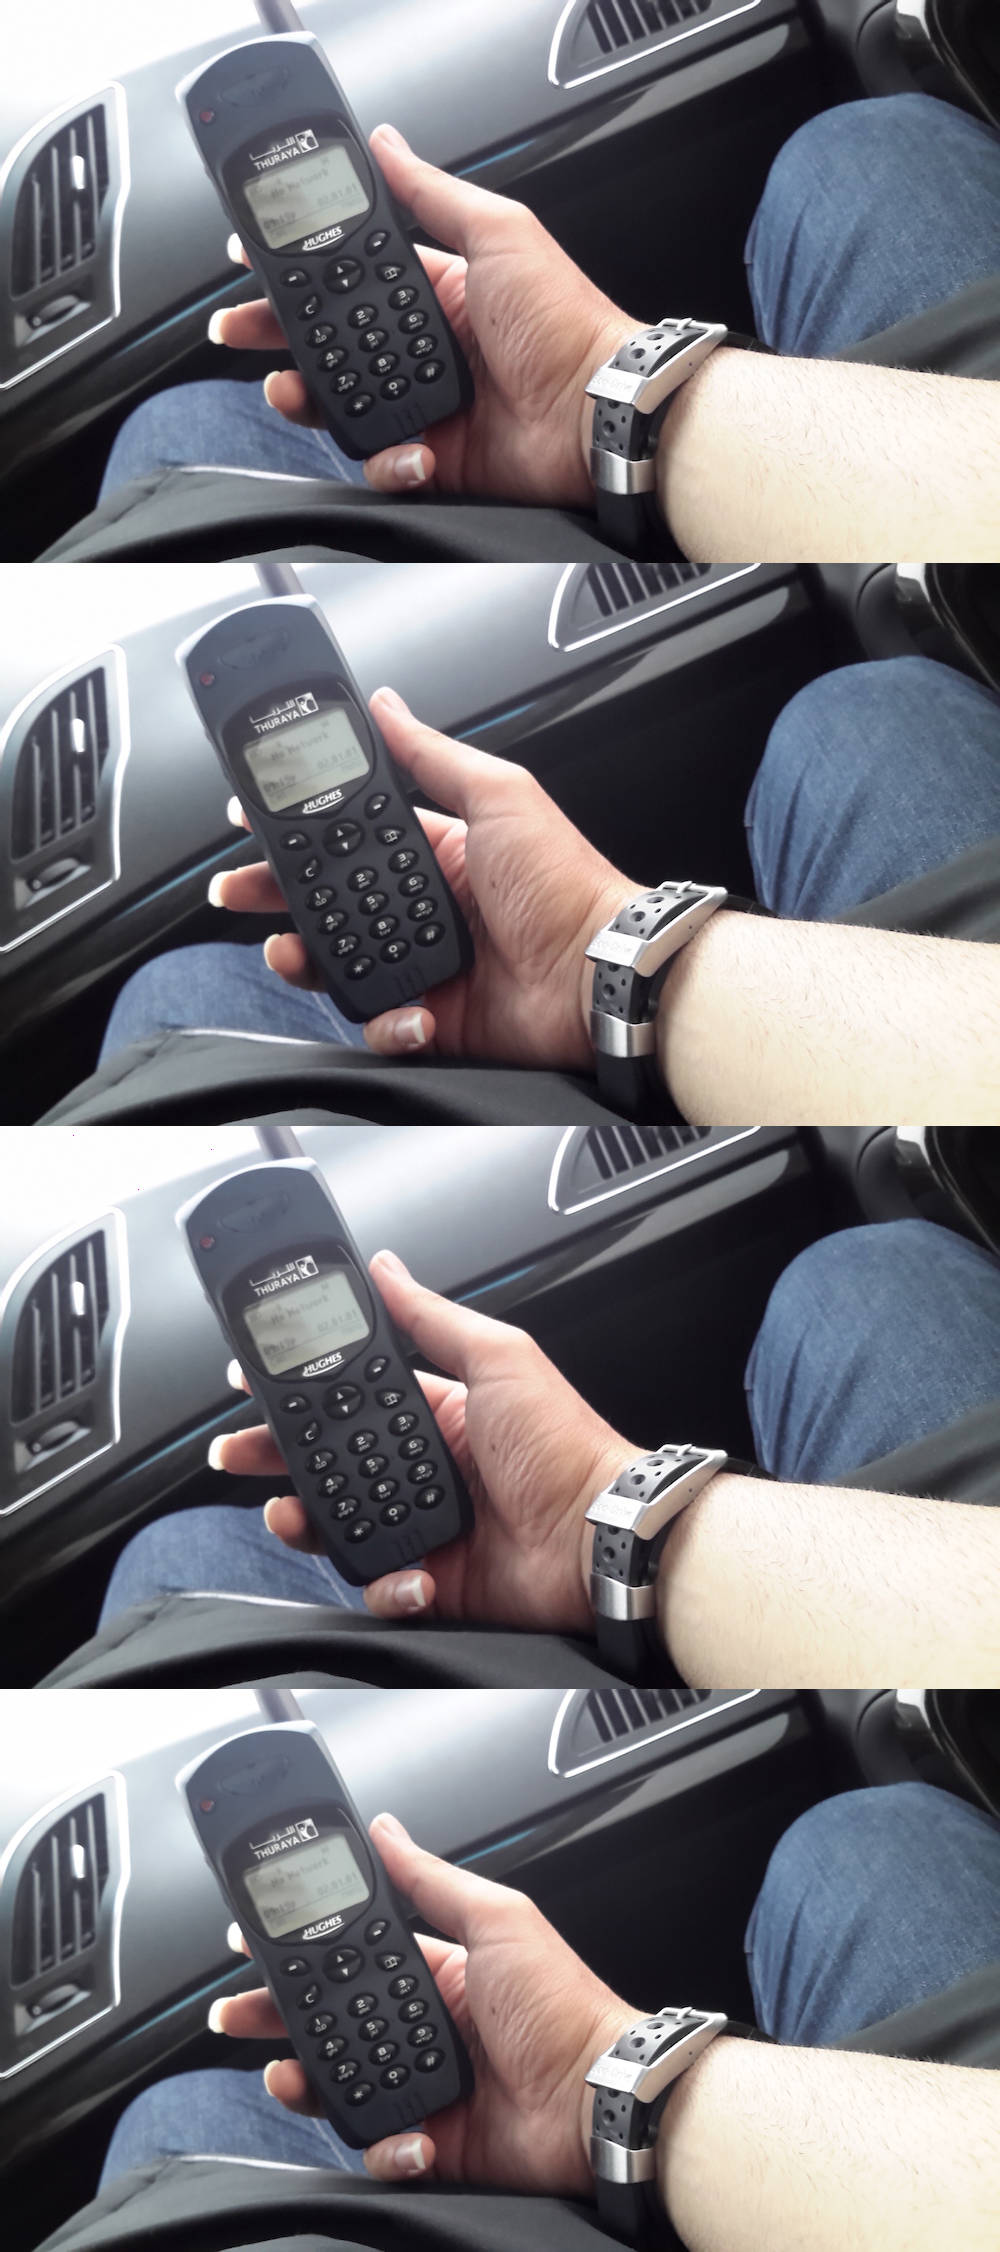
\includegraphics[width=0.7\textwidth]{./images/sat_phone_0.0001/wf_175_tef_040_rwf_045_original.png}
  \caption{Reconstruction of the Sat Phone Image Using \ac{CDP}s When the Relative Error is Almost $10^{-4}$ on all Color Channels\\
   From Top to Buttom: \ac{WF} at Iteration $175$, \ac{TWF} at Iteration $40$, \ac{RWF} at Iteration $45$, and the Original Image}
  \label{image:relative_error_0.0001}
  \end{figure}
  % \clearpage % End the page
}



On how the \ac{WF}\cite{Candes2014}\index{\ac{WF}} and the \ac{RWF}\cite{Zhang2016}\index{\ac{RWF}} are set to retrieve $\boldsymbol{x} \in \mathbb{C}^n$ up to a global phase 
please refer to \cref{pseudocode:wf} and \cref{pseudocode:rwf}. As it is evident from reconstruction of the sat phone image 
using \ac{CDP}\index{\ac{CDP}} in \cref{image:relative_error_0.0001}, the relative reconstruction error of $10^{-4}$ 
makes at least natural images quite indistinguishable when compared to the original image to the naked eye. If by unfolding/unrolling we can make 
the relative error some orders of magnitude smaller then the reconstructed images will become totally indistinguishable from the original image 
and we would be having \emph{outstandingly good} reconstruction instead of the \emph{good enough} reconstruction. The 
$L=160$ and $L=30$ are chosen with that incentive in mind(to have the relative error around $10^{-4}$ for the untrained \emph{unfolded}/\emph{unrolled} 
algorithms). Standing on the shoulders of giants \cite{Gregor2010} we try to get the said couple of orders of magnitude reduction in the relative 
error by tinkering with then update rule. 
\cite{Gregor2010}. The update rule in any \ac{WF}\cite{Liu2019}\cite{Jaganathan2015} variant in \cref{pseudocode:wf}, \ref{pseudocode:twf}, \ref{pseudocode:rwf}, \ref{pseudocode:irwf}, and \ref{pseudocode:imrwf} is of the form:
\begin{equation*}
  \boldsymbol{z}_{k+1} = \boldsymbol{z}_k - \tau\boldsymbol{\theta}[\boldsymbol{z}_k,\boldsymbol{A},\boldsymbol{A^*},\varphi]
\end{equation*}
where $\boldsymbol{\theta}[\boldsymbol{z}_k,\boldsymbol{A},\boldsymbol{A^*},\varphi]$ is a mapping that gives a vector as an output 
$\in\mathbb{C}^n$ and $\tau$ is the step size that was proposed by the respective algorithm. While just trying different mappings of the output vector might work 
some are more backed by theory and are worth exploring first. Changing the weight of the descent direction, by multiplying it by a scalar, is what most first-order adaptive gradient descent are doing in order to 
overcome the poor rate of convergence of the naive gradient descent. A linear transformation of the output vector by the means of a matrix-vector product is the next step 
and is the equivalent of finding better \emph{descent directions} or faster route to reach the minimum through changing of the \emph{scalar product} that induces our distance.
Assume that the algorithms are unfolded/unrolled $L$ times, 
we considered the following changes to the update rule and learning the associated parameters: 

\begin{enumerate}
  \item $\boldsymbol{z}_{k+1} = \boldsymbol{z}_k - \tau\boldsymbol{\theta}[\boldsymbol{z}_k,\boldsymbol{A},\boldsymbol{A^*},\varphi]$ 
  and learning the single scalar $\tau \in \mathbb{R}$ as to try and find a better gradient descent with constant step size,
  \item $\boldsymbol{z}_{k+1} = \boldsymbol{z}_k - \tau_k\boldsymbol{\theta}[\boldsymbol{z}_k,\boldsymbol{A},\boldsymbol{A^*},\varphi]$
  and learning $L$ scalars $\tau_k\in\mathbb{R}$ as to try and find a better adaptive gradient descent with large step sizes when possible 
  and small step sizes while being in \emph{stiff} regions, 
  \item $\boldsymbol{z}_{k+1} = \boldsymbol{z}_k - \boldsymbol{S}\boldsymbol{\theta}[\boldsymbol{z}_k,\boldsymbol{A},\boldsymbol{A^*},\varphi]$
  and learning a single semi-positive definite matrix $\boldsymbol{S}\in \mathbb{R}^{n\times n}$ as to try and find a better descent direction while 
  ensuring being always on the descent direction by the semi-positive definite constraint,
  \item $\boldsymbol{z}_{k+1} = \boldsymbol{z}_k - \boldsymbol{M}\boldsymbol{\theta}[\boldsymbol{z}_k,\boldsymbol{A},\boldsymbol{A^*},\varphi]$
  and learning a single general matrix $\boldsymbol{M}\in \mathbb{R}^{n\times n}$ as to try and find a better descent direction while 
  while not forcing the semi-positive definite constraint and hoping for the best,
  \item $\boldsymbol{z}_{k+1} = \boldsymbol{z}_k - \tau_k\boldsymbol{S}\boldsymbol{\theta}[\boldsymbol{z}_k,\boldsymbol{A},\boldsymbol{A^*},\varphi]$
  and learning a single semi-positive definite matrix $\boldsymbol{S}\in \mathbb{R}^{n\times n}$ and $L$ scalars $\tau_k \in \mathbb{R}$ as to try and find a 
  better descent direction with variable step sizes while \emph{trying} to ensure to be always on the descent direction by the semi-positive definite constraint(there is
  the possibility that the optimizer goes for a negative step sizes $\tau_k \in \mathbb{R}$), 
  \item $\boldsymbol{z}_{k+1} = \boldsymbol{z}_k - \tau_k\boldsymbol{M}\boldsymbol{\theta}[\boldsymbol{z}_k,\boldsymbol{A},\boldsymbol{A^*},\varphi]$
  and learning a single general matrix $\boldsymbol{M}\in \mathbb{R}^{n\times n}$ and $L$ scalars $\tau_k \in \mathbb{R}$ as to try and find a 
  better descent direction with variable step sizes while not forcing the semi-positive definite constraint and hoping for the best,
  \item $\boldsymbol{z}_{k+1} = \boldsymbol{z}_k - \boldsymbol{S}_k\boldsymbol{\theta}[\boldsymbol{z}_k,\boldsymbol{A},\boldsymbol{A^*},\varphi]$ 
  and learning $L$ semi-positive definite matrices $\boldsymbol{S}\in \mathbb{R}^{n\times n}$ as to try and find a better descent direction while 
  ensuring being always on the descent direction by the semi-positive definite constraint,
  \item $\boldsymbol{z}_{k+1} = \boldsymbol{z}_k - \boldsymbol{M}_k\boldsymbol{\theta}[\boldsymbol{z}_k,\boldsymbol{A},\boldsymbol{A^*},\varphi]$ 
  and learning $L$ general matrices $\boldsymbol{M}\in \mathbb{R}^{n\times n}$ as to try and find a better descent direction while 
  while not forcing the semi-positive definite constraint and hoping for the best,
\end{enumerate}
and we call them \emph{scenarios}. It is worth emphasizing that while from the parameter space point of view alone some scenarios are 
contained in others we explore them separately. The reasons include:

\begin{itemize}
  \item to come up with a model that has as few as possible parameters while still having 
  good performances on the train and the test data , which is one of the central ideas behind 
  \du/\au\cite{Shechtman2015}\index{\du}\index{\au}, and not a full blown general \ml/\dl model.
  \item not to confuse the optimizers unintentionally by introducing too many parameters \cite{Sankararaman2019}.
  \item not to overparameterize and in turn introducing overfitting\cite{Bishop2006}\cite{Goodfellow2016}\cite{ShalevShwartz2014}.
  \item not to burn too many \ac{FLOPS}\index{\ac{FLOPS}} needlessly.
\end{itemize}
As to stress the first bullet point the scenarios were sorted in the ascending order in terms of trainable parameters as one of our \emph{main} goals 
is to come up with a model with satisfactory improvement over the original algorithm by using as few as possible number of trainable parameters. 
The practitioner that wants to replicate the current study(or any other in the realm of \du/\au for that matter) is strongly encouraged to bid 
their time and start from scenario $1$ with $1$ trainable parameter and conclude with scenario $8$ with $Ln^2$ trainable parameters(or whatever 
that applies in their context).

During the training we go with the following setting:
\begin{itemize}
  \item initializing the trainable parameters in a way that at the beginning of the training the model coincides with the original iterative algorithm. 
  This is very crucial as in realistic settings the convergence of the original algorithm that is being \emph{unfolded}/\emph{unrolled} has conditions and 
  assumptions behind it which makes it is very dangerous to deviate from the proposed parameter setup. In fact during the prototyping phase of our own work 
  we faced divergence in the error before we even reached $1$ epoch 
  just because we forgot to act accordingly in the parameter setup that was proposed in the \ac{WF} and in the \ac{RWF}.    
  \item \adam\cite{Kingma2014}\index{\adam} as the optimizer with the starting 
  pseudo learning rate of $\mathrm{lr}=1.000\times10^{-3}$ which is 
  recommended\cite{Kingma2014}\cite{Sun2019}.
  \item taking $2$\cite{Masters2018} samples for the mini-batch stochastic gradient descent 
  that is wrapped inside \adam\cite{Kingma2014}\index{\adam}. Small batch sizes have the 
  disadvantage of introducing noise during the training process but at the same time make 
  the training process faster. They can also contribute to better generalization ability 
  of the \ml/\dl model \cite{Masters2018}.
  \item splitting the data into the train data and the test data with the ratio of $9$ to $1$ 
  in each epoch  not to overfit \cite{Goodfellow2016}\cite{Chollet2023}.
  \item tracking the relative error of the original algorithm \emph{unfolded}/\emph{unrolled} $L$ times 
  and the being trained network on train and test data as to decide on the generalization ability of the model \cite{Goodfellow2016}\cite{Chollet2023}.
\end{itemize}

The results of the training process for $50$ epochs for the first $3$ scenarios for the \ac{UWF} can be seen in \cref{fig:uwf_training_01_02_03}, the second $3$ scenarios in \cref{fig:uwf_training_04_05_06} and the 
last $2$ scenarios in \cref{fig:uwf_training_07_08_optuna} while keeping the pseudo learning rate the recommended $\mathrm{lr}=10^{-3}$ \cite{Kingma2014}\cite{Sun2019}. 
Similarly for the case of \ac{URWF} the results can be found in \cref{fig:urwf_training_01_02_03}, \cref{fig:urwf_training_04_05_06}, and \cref{fig:urwf_training_07_08_optuna}. 
In these figures we are looking for a couple of orders of magnitude decrease in the error for the model that is being trained both on the train 
and on the test data to ensure that our model has the much coveted \emph{generalizability} property. It can be seen some of the 
scenarios performed poorly(first scenario for both the \ac{UWF} and the \ac{URWF}) while some others were quite decent. The questions remains whether it is possible 
to get better results by changing the pseudo learning rate($\mathrm{lr}$) even for the case of the first scenario or more importantly 
for which one of the scenarios and what pseudo learning rate($\mathrm{lr}$) can we achieve the best performance? The stated concerns to some extent can be answered by the means of a 
\ho \cite{Hutter2019}\cite{Akiba2019} study. \HO studies help the \ml/\dl practitioners to fine-tune their models and come up with better and better set of 
parameters. \HO relies on searching through a parameter space to look for a suitable set of parameters. A parameter space is basically the cartesian 
products of the range of the parameters. Obviously the resulting set must be countable otherwise it would take infinite FLOPS and in turn infinite time to 
reach the set of parameters for the best model. That is why when facing a continuous parameter like the pseudo learning rate($\mathrm{lr}$) 
in our case the parameter must be discretized or sampled with a sampler. Discussion of the technics in the \ho realm is quite 
involved, but it should be pointed out that the level of theory backing up the \ho is somewhere between brute force methods and mathematical optimization. 
While a crude grid search and comparison in our case using the combination of \bash\cite{Ramey2022}\index{\bash}(looping over 
the grid points) and \awk\cite{Robbins2023}\index{\awk}(lazy database management for bookkeeping) could be used due to our 
small parameter space, we settled on using a domain specific package for the \ho\cite{Hutter2019}\cite{Akiba2019}\index{\ho} 
part. There are quite a number of packages that can be used for \ho\cite{Hutter2019}\cite{Akiba2019}\index{\ho} and we took the decision to go with 
\optuna\cite{Akiba2019}\index{\optuna}. Our reasons for using the \optuna\cite{Akiba2019}\index{\optuna} include but not limited to:
\begin{itemize}
  \item Use of the latest technics in \ho\cite{Hutter2019}\cite{Akiba2019}\index{\ho}.
  \item It is quite lightweight.
  \item Describing the parameter space is both easy and flexible \cite{Akiba2019}.
  \item Pruning capabilities for not-so-optimistic scenarios by implanting probes(measuring some value to decide on early stopping) \cite{Akiba2019}.
  \item Distributed computing can be done thanks to the \ac{RDBMS}s. At the $2019$ \scipy conference, the \optuna team stated that their implementation can handle up to $6$ computational nodes in the case of distributed computing.
  \item Usage of \ac{RDBMS} for bookkeeping, safekeeping(in case of crash or just rebooting) and handling of dead-locks associated with the distributed computing.
  \item Nice dashboard for better visualization and interpretation of the results.  
\end{itemize}
The range of scenarios is obvious but what about the pseudo learning rate($\mathrm{lr}$)? 
During the prototyping we observed that the $\mathrm{lr}=10^{-2}$ would result in the error exploding and $\mathrm{lr}=10^{-4}$ would perform 
inferior to the already observed $\mathrm{lr}=10^{-3}$ and that is why we set $\mathrm{lr}=10^{-4}$ and $\mathrm{lr}=10^{-2}$ 
as the lower and upper bounds on the pseudo learning rate($\mathrm{lr}$). We chose the uniform sampler for discretization of the pseudo learning rate($\mathrm{lr}$). 
Now comes the easy part where you can sit back and let the \optuna\cite{Akiba2019} go over the discrete grid at its own discretion(\ho technics \cite{Hutter2019}\cite{Akiba2019}).
After \ho\cite{Hutter2019}\cite{Akiba2019}\index{\ho} while focusing on scenarios and the pseudo learning rate($\mathrm{lr}$) in \adam\cite{Kingma2014} 
we arrive at the final proposed best scenario for the \ac{UWF} in the third subfigure of \cref{fig:uwf_training_07_08_optuna} and for the 
\ac{URWF} in the third subfigure of \cref{fig:urwf_training_07_08_optuna}. It can be seen that we were successful to reduce the error both on the train and the test data and the decrease is better that the originally models trained with $\mathrm{lr}=10^{-3}$ 
thanks to the \ho study. While it might sound like a contradiction that trained \emph{unfolded}/\emph{unrolled} supervisor \ac{RWF} algorithm
is performing similarly to the trained \emph{unfolded}/\emph{unrolled} \ac{WF} algorithm the reader must recall that \ac{RWF} is only \emph{unfolded}/\emph{unrolled} $30$ times while 
the \ac{WF} is \emph{unfolded}/\emph{unrolled} $160$ times. 

%%%%%%%%%%%%%%%%%%%%%%%%%%%%%%%%%%%%%%%%%%%%%%%%%%%%%%%%%%%%%
%%%%% Training UWF Without Hyperparameter Optimization %%%%%%
%%%%%%%%%%%%%%%%%%%%%%%%%%%%%%%%%%%%%%%%%%%%%%%%%%%%%%%%%%%%%
\afterpage{%
%   \clearpage % Start a new page
\begin{figure}[!htbp]
  \subfloat[Single Scalar$(\tau)$, $\mathrm{lr}=1.000\times10^{-3}, \,\mathrm{L}=160$]{% This file was created with tikzplotlib v0.10.1.
\begin{tikzpicture}

  \definecolor{darkgray176}{RGB}{176,176,176}
  \definecolor{green}{RGB}{0,128,0}
  \definecolor{lightgray204}{RGB}{204,204,204}
  \definecolor{orange}{RGB}{255,165,0}
  
  \begin{axis}[
    width = 0.95\textwidth,
    height = 18em,
  legend cell align={left},
  legend style={
    fill opacity=0.8,
    draw opacity=1,
    text opacity=1,
    % at={(0.91,0.5)},
    % anchor=east,
    draw=lightgray204
  },
  % log basis y={10},
  tick align=outside,
  tick pos=left,
  title={Average Error vs Epochs},
  x grid style={darkgray176},
  xlabel={Epochs},
  xmajorgrids,
  xmin=-2.45, xmax=51.45,
  xtick style={color=black},
  y grid style={darkgray176},
  ylabel={Average Error},
  ymajorgrids,
  ymin=1.13394664622616e-05, ymax=0.161938808815307,
ymode=log,
ytick style={color=black},
ytick={1e-06,1e-05,0.0001,0.001,0.01,0.1,1,10},
yticklabels={
  \(\displaystyle {10^{-6}}\),
  \(\displaystyle {10^{-5}}\),
  \(\displaystyle {10^{-4}}\),
  \(\displaystyle {10^{-3}}\),
  \(\displaystyle {10^{-2}}\),
  \(\displaystyle {10^{-1}}\),
  \(\displaystyle {10^{0}}\),
  \(\displaystyle {10^{1}}\)
}
]
\addplot [ultra thick, red]
table {%
0 0.000115964649012312
1 0.000106160565337632
2 7.4514202424325e-05
3 5.52686251467094e-05
4 6.47887063678354e-05
5 4.38010902144015e-05
6 3.23934727930464e-05
7 2.78183033515234e-05
8 3.57124663423747e-05
9 3.53135837940499e-05
10 3.40799015248194e-05
11 3.13175551127642e-05
12 3.11450057779439e-05
13 3.30704897351097e-05
14 3.04046770907007e-05
15 2.96264006465208e-05
16 5.87791255384218e-05
17 5.6647138990229e-05
18 0.0146533735096455
19 2.88673472823575e-05
20 2.93554567178944e-05
21 2.82165401586099e-05
22 2.787177436403e-05
23 3.11427174892742e-05
24 2.85501137113897e-05
25 3.01203654089477e-05
26 2.84152793028625e-05
27 2.73057776212227e-05
28 2.64660557149909e-05
29 2.9429202186293e-05
30 2.62424036918674e-05
31 2.8169297365821e-05
32 5.54843718418851e-05
33 4.05666069127619e-05
34 2.75754628091818e-05
35 2.71147255261894e-05
36 2.93161992885871e-05
37 2.23202241613762e-05
38 6.3687919464428e-05
39 3.87190993933473e-05
40 2.34123890550109e-05
41 2.28933477046667e-05
42 2.15512700378895e-05
43 2.40790013776859e-05
44 2.48580217885319e-05
45 2.92275672109099e-05
46 2.18897512240801e-05
47 2.32488600886427e-05
48 2.91028009087313e-05
49 2.16724984056782e-05
};
\addlegendentry{During Training on Train Data}
\addplot [ultra thick, blue]
table {%
0 0.000119965603516903
1 0.000101332203485072
2 6.76928320899606e-05
3 6.92283501848578e-05
4 6.13137017353438e-05
5 3.69310146197677e-05
6 4.69658516522031e-05
7 3.3255073503824e-05
8 2.56295552389929e-05
9 2.45451210503234e-05
10 4.22778066422325e-05
11 2.65813923761016e-05
12 2.23145234485855e-05
13 8.61937660374679e-05
14 3.43234569299966e-05
15 2.67034629359841e-05
16 2.29790675803088e-05
17 2.527412470954e-05
18 3.0333951144712e-05
19 4.13999114243779e-05
20 4.60761657450348e-05
21 6.34397874819115e-05
22 3.28440728480928e-05
23 2.81884076684946e-05
24 0.10483306646347
25 3.2550346077187e-05
26 6.62766105961055e-05
27 3.55897900590207e-05
28 3.84878294426017e-05
29 3.16521618515253e-05
30 4.70157174277119e-05
31 2.27859763981542e-05
32 2.39355322264601e-05
33 3.09546412609052e-05
34 2.7367514121579e-05
35 3.2791547710076e-05
36 0.000126061495393515
37 3.74597329937387e-05
38 2.36853138630977e-05
39 3.31944938807283e-05
40 2.21443497139262e-05
41 4.30283471359871e-05
42 2.20024030568311e-05
43 2.08455585379852e-05
44 3.03072501992574e-05
45 2.1999707314535e-05
46 2.23901915887836e-05
47 2.24012856051559e-05
48 1.75164168467745e-05
49 3.0965751648182e-05
};
\addlegendentry{During Training on Test Data}
\addplot [ultra thick, orange]
table {%
0 0.00232795067131519
1 0.000121869074064307
2 0.000120698474347591
3 0.000135069276439026
4 0.0124339954927564
5 0.000153945249621756
6 0.000118231007945724
7 0.000122039848065469
8 0.000140186384669505
9 0.00012726680142805
10 0.000174994856934063
11 0.000118236494017765
12 0.000121040582598653
13 0.000119276381155942
14 0.000180863629793748
15 0.00012022288137814
16 0.000117313240480144
17 0.00351618696004152
18 0.000130253116367385
19 0.00012056008563377
20 0.000164105353178456
21 0.0109988208860159
22 0.000125871316413395
23 0.000133313849801198
24 0.000120252356282435
25 0.000160284704179503
26 0.000125728212879039
27 0.000121358069009148
28 0.000733525725081563
29 0.000154539637151174
30 0.000126869344967417
31 0.000736654968932271
32 0.000129571038996801
33 0.000122085199109279
34 0.000125906270113774
35 0.000116696552140638
36 0.000130216154502705
37 0.000120131124276668
38 0.000999922631308436
39 0.000127725084894337
40 0.000121914374176413
41 0.000124539728858508
42 0.000120200413221028
43 0.000201997492695227
44 0.000120335920655634
45 0.000125129503430799
46 0.000128802537801675
47 0.000120474636787549
48 0.00011976600944763
49 0.00018517866556067
};
\addlegendentry{Untrained Model on Train Data}
\addplot [ultra thick, green]
table {%
0 0.000129062638734467
1 0.000145741840242408
2 0.000148645412991755
3 0.000185903554665856
4 9.62841222644784e-05
5 0.00011643586185528
6 0.000125509759527631
7 0.000164188357302919
8 0.000113728274300229
9 0.000184246688149869
10 0.000108123131212778
11 0.000156331152538769
12 0.000132504908833653
13 0.00010812053369591
14 0.000102231824712362
15 0.000158902883413248
16 0.000109439031803049
17 0.000112151916255243
18 0.000105350838566665
19 0.000150613894220442
20 0.000124783167848364
21 0.000110051209048834
22 0.000146668040542863
23 0.00042110844515264
24 0.000153782195411623
25 0.000121453274914529
26 0.000192303283256479
27 0.000158814698806964
28 0.000107618201582227
29 0.00013192389451433
30 0.000138851260999218
31 0.000123196819913574
32 0.000149802639498375
33 0.000124568658065982
34 8.8295120804105e-05
35 0.000161883814143948
36 0.000107056694105268
37 0.000165244477102533
38 0.000120437529403716
39 0.000129807071061805
40 0.000140801450470462
41 0.000128936153487302
42 0.000151907806866802
43 0.000133040055516176
44 0.000141951051773503
45 0.000136660790303722
46 0.000119454423838761
47 0.000174097032868303
48 0.000137830531457439
49 0.000133577806991525
};
\addlegendentry{Untrained Model on Test Data}
\end{axis}

\end{tikzpicture}
}\\
  \subfloat[Different Scalars$(\tau_k)$, $\mathrm{lr}=1.000\times10^{-3}, \,\mathrm{L}=160$]{% This file was created with tikzplotlib v0.10.1.
\begin{tikzpicture}

    \definecolor{darkgray176}{RGB}{176,176,176}
    \definecolor{green}{RGB}{0,128,0}
    \definecolor{lightgray204}{RGB}{204,204,204}
    \definecolor{orange}{RGB}{255,165,0}
    
    \begin{axis}[
      width = 0.95\textwidth,
      height = 19em,
    legend cell align={left},
    legend style={
      fill opacity=0.8,
      draw opacity=1,
      text opacity=1,
      % at={(0.91,0.5)},
      % anchor=east,
      draw=lightgray204
    },
    % log basis y={10},
    tick align=outside,
    tick pos=left,
    title={Average Error vs Epochs},
    x grid style={darkgray176},
    xlabel={Epochs},
    xmajorgrids,
    xmin=-2.45, xmax=51.45,
    xtick style={color=black},
    y grid style={darkgray176},
    ylabel={Average Error},
    ymajorgrids,
    ymin=1.77265045649501e-06, ymax=0.0217257085799638,
ymode=log,
ytick style={color=black},
ytick={1e-07,1e-06,1e-05,0.0001,0.001,0.01,0.1,1},
yticklabels={
  \(\displaystyle {10^{-7}}\),
  \(\displaystyle {10^{-6}}\),
  \(\displaystyle {10^{-5}}\),
  \(\displaystyle {10^{-4}}\),
  \(\displaystyle {10^{-3}}\),
  \(\displaystyle {10^{-2}}\),
  \(\displaystyle {10^{-1}}\),
  \(\displaystyle {10^{0}}\)
}
]
\addplot [ultra thick, red]
table {%
0 0.000116249197162688
1 0.000104777733213268
2 6.16174802416936e-05
3 5.35397994099185e-05
4 4.22738339693751e-05
5 4.02698206016794e-05
6 3.1009447411634e-05
7 3.72181639249902e-05
8 2.38204429479083e-05
9 2.01366219698684e-05
10 1.8768372683553e-05
11 2.01797083718702e-05
12 1.48041463035042e-05
13 1.4403810382646e-05
14 0.00846845842897892
15 1.27274661281263e-05
16 4.39258001279086e-05
17 1.06620564110926e-05
18 1.03143329397426e-05
19 1.32283394123078e-05
20 8.70245912665268e-06
21 7.9739720604266e-06
22 7.91216280049412e-06
23 7.81663038651459e-06
24 7.15070973456022e-06
25 7.19865693099564e-06
26 6.38139272268745e-06
27 6.38953406451037e-06
28 7.23988569006906e-06
29 0.01416249666363
30 5.43188207302592e-06
31 5.12640826855204e-06
32 5.32065496372525e-06
33 5.13297209181474e-06
34 5.40986866326421e-06
35 0.00397870503365993
36 4.45748082711361e-06
37 4.19193565903697e-06
38 4.29415240432718e-06
39 4.04746242566034e-06
40 4.57452460977947e-06
41 4.86139288113918e-06
42 5.43156011190149e-06
43 3.66582253263914e-06
44 3.54837652594142e-06
45 3.25559403790976e-06
46 3.63603157893522e-06
47 3.86781039196649e-06
48 3.25598648487357e-06
49 2.61864806816448e-05
};
\addlegendentry{During Training on Train Data}
\addplot [ultra thick, blue]
table {%
0 0.000112263674964197
1 8.04891242296435e-05
2 8.31869256217033e-05
3 5.98654623900075e-05
4 4.89498270326294e-05
5 3.72918257198762e-05
6 3.3739663194865e-05
7 2.4729093638598e-05
8 2.31083031394519e-05
9 2.10517519008135e-05
10 1.91858325706562e-05
11 2.23716870095814e-05
12 2.35791285376763e-05
13 1.72630680026487e-05
14 1.55992747750133e-05
15 1.44481573443045e-05
16 1.11354383989237e-05
17 1.27217863337137e-05
18 1.25628239402431e-05
19 1.01310497484519e-05
20 9.15393957257038e-06
21 1.09975608211244e-05
22 1.18624620881747e-05
23 6.98091344020213e-06
24 6.74611374051892e-06
25 7.77813875174616e-06
26 7.35434741727659e-06
27 0.000388607470085844
28 7.51973493606783e-06
29 6.748153737135e-06
30 5.72535964238341e-06
31 7.17473221811815e-06
32 4.50263542006724e-06
33 4.60407500213478e-06
34 4.90940510644577e-06
35 4.40480425822898e-06
36 5.02696912008105e-06
37 5.87127215112559e-06
38 2.96681491818163e-06
39 4.38676352132461e-06
40 6.17989599049906e-06
41 5.71354394196533e-06
42 8.28803877084283e-06
43 4.08831328968517e-06
44 3.16428372570954e-06
45 4.80631888422067e-06
46 3.29530416820489e-06
47 3.25893643093877e-06
48 2.71930070994131e-06
49 3.02756961900741e-06
};
\addlegendentry{During Training on Test Data}
\addplot [ultra thick, orange]
table {%
0 0.000120269258331973
1 0.000117629810119979
2 0.000122440571431071
3 0.000114334048703313
4 0.000114169095468242
5 0.000116113071271684
6 0.000115084993012715
7 0.000130586326122284
8 0.000293938588583842
9 0.000122917335829698
10 0.00013070237764623
11 0.000482346513308585
12 0.000111455316073261
13 0.000112260117020924
14 0.000119041971629485
15 0.000120722070278134
16 0.00012233828601893
17 0.000125074948300608
18 0.000120170683658216
19 0.00011924283899134
20 0.000114032402052544
21 0.000119969517982099
22 0.000120646553114057
23 0.000115742535854224
24 0.000115109338366892
25 0.00161717541050166
26 0.00751296384260058
27 0.000110919230792206
28 0.00012136172153987
29 0.000134457382955588
30 0.000120748292829376
31 0.000121317578305025
32 0.000110163149656728
33 0.00011455421190476
34 0.000116186180093791
35 0.000116979601443745
36 0.000121848745038733
37 0.000116133829578757
38 0.000113216083263978
39 0.000117256036901381
40 0.000131090360810049
41 0.000154755791299976
42 0.000118435942567885
43 0.000119846772577148
44 0.000113804286229424
45 0.000124071579193696
46 0.000145310332300141
47 0.000177828187588602
48 0.000121933335321955
49 0.000113341317046434
};
\addlegendentry{Untrained Model on Train Data}
\addplot [ultra thick, green]
table {%
0 0.000106313964352012
1 0.000105647886812221
2 0.000103366750408895
3 0.000113759066152852
4 0.000132218236103654
5 0.000128917745314538
6 9.70740729826503e-05
7 0.000144520294270478
8 0.00013117839989718
9 0.000100422148534562
10 0.000251530116656795
11 0.000114149901492056
12 0.000155831527081318
13 0.000131669556139968
14 0.000102509882708546
15 0.000113139096356463
16 0.000115782873763237
17 0.000102498932392336
18 0.000134782283566892
19 0.000123556092148647
20 0.000126511658891104
21 0.000114194604975637
22 0.000122136902064085
23 0.000116400944534689
24 0.000121366094390396
25 7.6622687629424e-05
26 0.000139483527163975
27 0.000126818413264118
28 0.000112633853859734
29 0.000108447231468745
30 0.000130197833641432
31 0.000123179153888486
32 0.000150192689034157
33 0.000118637071864214
34 0.000123824764159508
35 8.92329844646156e-05
36 0.000178371163201518
37 0.000124380996567197
38 0.000136194779770449
39 0.000112504290882498
40 0.000124128026072867
41 0.000127703809994273
42 9.60812903940678e-05
43 0.000133860929054208
44 9.82828350970522e-05
45 0.000132986911921762
46 0.00011109155457234
47 0.000109223496110644
48 0.000132101107737981
49 0.000131110078655183
};
\addlegendentry{Untrained Model on Test Data}
\end{axis}

\end{tikzpicture}
}\\
  \subfloat[Single Matrix$(\boldsymbol{M})$, $\mathrm{lr}=1.000\times10^{-3}, \,\mathrm{L}=160$]{% This file was created with tikzplotlib v0.10.1.
\begin{tikzpicture}

  \definecolor{darkgray176}{RGB}{176,176,176}
  \definecolor{green}{RGB}{0,128,0}
  \definecolor{lightgray204}{RGB}{204,204,204}
  \definecolor{orange}{RGB}{255,165,0}
  
  \begin{axis}[
    width = 0.95\textwidth,
    height = 19em,
  legend cell align={left},
  legend style={
    fill opacity=0.8,
    draw opacity=1,
    text opacity=1,
    at={(0.91,0.5)},
    anchor=east,
    draw=lightgray204
  },
  % log basis y={10},
  tick align=outside,
  tick pos=left,
  title={Average Error vs Epochs},
  x grid style={darkgray176},
  xlabel={Epochs},
  xmajorgrids,
  xmin=-2.45, xmax=51.45,
  xtick style={color=black},
  y grid style={darkgray176},
  ylabel={Average Error},
  ymajorgrids,
  ymin=1.37307878496665e-06, ymax=0.177846155019824,
ymode=log,
ytick style={color=black},
ytick={1e-07,1e-06,1e-05,0.0001,0.001,0.01,0.1,1,10},
yticklabels={
  \(\displaystyle {10^{-7}}\),
  \(\displaystyle {10^{-6}}\),
  \(\displaystyle {10^{-5}}\),
  \(\displaystyle {10^{-4}}\),
  \(\displaystyle {10^{-3}}\),
  \(\displaystyle {10^{-2}}\),
  \(\displaystyle {10^{-1}}\),
  \(\displaystyle {10^{0}}\),
  \(\displaystyle {10^{1}}\)
}
]
\addplot [ultra thick, red]
table {%
0 0.000100550205388572
1 5.51480588910636e-05
2 3.5376513551455e-05
3 2.45903993345564e-05
4 1.96682776731905e-05
5 2.25053372560069e-05
6 1.78705213329522e-05
7 1.38656941999216e-05
8 2.33041700994363e-05
9 1.75389577634633e-05
10 1.20915501611307e-05
11 1.22163710329914e-05
12 3.94555172533728e-05
13 9.94717083813157e-06
14 8.66588470671559e-06
15 8.12911912362324e-06
16 8.36843628349015e-06
17 4.37713715655264e-05
18 7.10201402398525e-06
19 8.66146274347557e-06
20 6.56404654364451e-06
21 6.46528542347369e-06
22 6.1509813349403e-06
23 7.15849364496535e-06
24 6.78525930197793e-06
25 6.03655644226819e-06
26 7.20456819180981e-06
27 6.27475947112544e-06
28 5.21144374943106e-06
29 5.08226366946474e-06
30 5.34771334059769e-06
31 5.64463289265404e-06
32 5.18060278409394e-06
33 6.93121137373964e-06
34 4.74545822726213e-06
35 4.78483070764923e-06
36 7.58898931962904e-06
37 7.7153699749033e-06
38 7.95855885371566e-06
39 4.45058958575828e-06
40 4.64240429209895e-06
41 4.50455945610884e-06
42 0.000109414861071855
43 7.1724243753124e-06
44 6.40393318462884e-06
45 6.23621372142225e-06
46 6.10479764873162e-06
47 6.92588446327136e-06
48 5.43964370081085e-06
49 5.19705054102815e-06
};
\addlegendentry{During Training on Train Data}
\addplot [ultra thick, blue]
table {%
0 0.000120791839435697
1 6.97270734235644e-05
2 3.00260344374692e-05
3 2.56979237747146e-05
4 7.61366973165423e-05
5 2.01856510102516e-05
6 1.7695394490147e-05
7 1.28419051179662e-05
8 1.4239049050957e-05
9 1.02809890449862e-05
10 9.40511290536961e-06
11 9.17238776310114e-06
12 1.02190724646789e-05
13 1.52930533658946e-05
14 8.76629474078072e-06
15 4.00103817810304e-05
16 7.77208060753765e-06
17 1.29295967781218e-05
18 1.09010425148881e-05
19 5.81508083996596e-06
20 6.4081177697517e-06
21 5.60884700462339e-06
22 6.61514650346362e-06
23 5.13239729116322e-06
24 3.91138337363373e-06
25 3.8252628655755e-06
26 4.53538950750954e-06
27 6.18455396761419e-06
28 1.11798572106636e-05
29 4.6780855882389e-06
30 5.49044807485188e-06
31 3.70292764273472e-06
32 5.24500364917913e-06
33 3.88661010219948e-06
34 3.4318647976761e-06
35 3.57546377927065e-06
36 2.76254536402121e-06
37 3.40951532962208e-06
38 2.6036304916488e-06
39 3.45822490999126e-06
40 2.34463345805125e-06
41 2.62418188867741e-06
42 1.0984908840328e-05
43 7.6518654168467e-06
44 6.64355184198939e-06
45 5.13065879204078e-06
46 4.27781515099923e-06
47 5.18121805725968e-06
48 4.84617430629442e-06
49 4.89258400193648e-06
};
\addlegendentry{During Training on Test Data}
\addplot [ultra thick, orange]
table {%
0 0.00010484314407222
1 0.000107949126686435
2 0.000103496546216775
3 0.00010804993507918
4 0.000110162152850535
5 0.000296750164125115
6 0.00010558851499809
7 0.000139229741762392
8 0.000106780855276156
9 0.000106322971987538
10 0.000102692516520619
11 0.000109833126771264
12 0.00010538525384618
13 0.000106810737634078
14 0.000102086036349647
15 0.000116774193884339
16 0.000119435600936413
17 0.000102182850241661
18 0.000102641686680727
19 0.00530683295801282
20 0.000103274374851026
21 0.000103942598798312
22 0.000103939244581852
23 0.000104276216006838
24 0.000110928223875817
25 0.000103578386188019
26 0.000103336431493517
27 0.000105195016658399
28 0.000104166712844744
29 0.000104556929727551
30 0.000103958751424216
31 0.00010203668352915
32 0.0128590352833271
33 0.000113665089884307
34 0.000115690469101537
35 0.000104450569779146
36 0.000209172590984963
37 0.000118048126751091
38 0.0001468143746024
39 0.000105119623185601
40 0.000103922306152526
41 0.000104989230749197
42 0.000103922313428484
43 0.000509256205987185
44 0.000105649472970981
45 0.000173034990439191
46 0.000102450037957169
47 0.00010490239947103
48 0.000103624282928649
49 0.000105106271803379
};
\addlegendentry{Untrained Model on Train Data}
\addplot [ultra thick, green]
table {%
0 0.000162609125254676
1 8.71792071848176e-05
2 0.000132129905978218
3 0.000102534242614638
4 9.55780051299371e-05
5 0.000103471626061946
6 0.00011843147512991
7 0.000143871642649174
8 9.12305331439711e-05
9 0.000115696624561679
10 0.000134690388222225
11 0.000117837000289001
12 0.00011143229494337
13 9.86462255241349e-05
14 0.000122453842777759
15 0.000104537131846882
16 0.000188419173355214
17 0.000112128611363005
18 0.000126249200548045
19 0.000111318797280546
20 0.000138589079142548
21 0.000112062720290851
22 0.000109058710222598
23 0.000148940816870891
24 8.78246864886023e-05
25 0.00011311150592519
26 0.000116243281809147
27 0.00012264410906937
28 0.000129606036352925
29 0.000117648742161691
30 9.57143638515845e-05
31 0.000130468906718306
32 0.000118919684609864
33 0.0001254016533494
34 0.000107390391349327
35 0.00010970434959745
36 9.73197384155355e-05
37 0.000118234478577506
38 0.000114819522423204
39 9.58838500082493e-05
40 0.000119389638712164
41 9.30892638280056e-05
42 0.000110404413135257
43 0.000113703594252001
44 0.104151368141174
45 0.000135112306452356
46 0.000178929112735204
47 0.000112616180558689
48 0.000114114074676763
49 0.000113444977614563
};
\addlegendentry{Untrained Model on Test Data}
\end{axis}

\end{tikzpicture}
}\\  
  \caption{\ac{UWF}\index{UWF} Training in Different Scenarios Without \optuna\cite{Akiba2019}}
  \label{fig:uwf_training_01_02_03}
  \end{figure}
%   \clearpage % End the page
}
\afterpage{%
%   \clearpage % Start a new page
\begin{figure}[!htbp]
  \subfloat[Single Semi-Positive Definite Matrix$(\boldsymbol{S})$, $\mathrm{lr}=1.000\times10^{-3}, \,\mathrm{L}=160$]{% This file was created with tikzplotlib v0.10.1.
\begin{tikzpicture}

  \definecolor{darkgray176}{RGB}{176,176,176}
  \definecolor{green}{RGB}{0,128,0}
  \definecolor{lightgray204}{RGB}{204,204,204}
  \definecolor{orange}{RGB}{255,165,0}
  
  \begin{axis}[
    width = 0.95\textwidth,
    height = 19em,
  legend cell align={left},
  legend style={
    fill opacity=0.8,
    draw opacity=1,
    text opacity=1,
    at={(0.91,0.5)},
    anchor=east,
    draw=lightgray204
  },
  % log basis y={10},
  tick align=outside,
  tick pos=left,
  title={Average Error vs Epochs},
  x grid style={darkgray176},
  xlabel={Epochs},
  xmajorgrids,
  xmin=-2.45, xmax=51.45,
  xtick style={color=black},
  y grid style={darkgray176},
  ylabel={Average Error},
  ymajorgrids,
  ymin=8.30356451495163e-07, ymax=0.0234483376377019,
  ymode=log,
  ytick style={color=black},
  ytick={1e-08,1e-07,1e-06,1e-05,0.0001,0.001,0.01,0.1,1},
  yticklabels={
    \(\displaystyle {10^{-8}}\),
    \(\displaystyle {10^{-7}}\),
    \(\displaystyle {10^{-6}}\),
    \(\displaystyle {10^{-5}}\),
    \(\displaystyle {10^{-4}}\),
    \(\displaystyle {10^{-3}}\),
    \(\displaystyle {10^{-2}}\),
    \(\displaystyle {10^{-1}}\),
    \(\displaystyle {10^{0}}\)
  }
  ]
  \addplot [ultra thick, red]
  table {%
  0 0.00011017140786862
  1 4.11059882026166e-05
  2 2.26791598834097e-05
  3 1.79246799234534e-05
  4 1.5320852980949e-05
  5 1.33630046548205e-05
  6 9.5052946562646e-06
  7 7.66472021496156e-06
  8 6.61656895317719e-06
  9 0.0147163737565279
  10 5.08682569488883e-06
  11 6.89014314048109e-06
  12 4.54574956165743e-06
  13 4.62558455183171e-06
  14 4.29807005275507e-06
  15 3.20831509270647e-06
  16 3.78796448785579e-06
  17 3.14419253300002e-06
  18 2.96950793199358e-06
  19 2.8898784876219e-06
  20 3.10484847432235e-06
  21 2.37921130974428e-06
  22 2.31052422350331e-06
  23 4.23871242674068e-05
  24 2.47495540861564e-06
  25 4.16208604292478e-06
  26 1.87935143003415e-06
  27 2.81569600701914e-06
  28 2.99561907013413e-06
  29 1.83097131412069e-06
  30 2.34298590839899e-06
  31 0.00187448516953737
  32 0.00130452052690089
  33 0.00114362325984985
  34 0.00110848690383136
  35 0.000213812745641917
  36 0.000175953828147613
  37 0.000123330348287709
  38 0.000108028660179116
  39 8.94952609087341e-05
  40 8.3952174463775e-05
  41 7.61759874876589e-05
  42 6.94747795932926e-05
  43 5.97251892031636e-05
  44 5.72363132960163e-05
  45 4.79114059999119e-05
  46 4.97014989377931e-05
  47 4.38004644820467e-05
  48 4.24669815402012e-05
  49 3.88910702895373e-05
  };
  \addlegendentry{During Training on Train Data}
  \addplot [ultra thick, blue]
  table {%
  0 9.25490385270678e-05
  1 5.33596867171582e-05
  2 1.93084251804976e-05
  3 1.55448160512606e-05
  4 1.25676324387314e-05
  5 1.28699921333464e-05
  6 7.57245152271935e-06
  7 6.81047959005809e-06
  8 6.69457676849561e-06
  9 5.67144479646231e-06
  10 3.838911652565e-06
  11 4.25930056735524e-06
  12 3.28157580042898e-06
  13 3.14029966830276e-06
  14 3.49249467035406e-06
  15 3.93286927646841e-06
  16 1.021505886456e-05
  17 2.12089162232587e-06
  18 3.26139775097545e-06
  19 2.53603025157645e-06
  20 2.11525298254855e-06
  21 2.54228211815644e-06
  22 1.61134596510237e-06
  23 1.71185638464522e-06
  24 1.63372749284463e-06
  25 1.61897480666084e-06
  26 1.4033945490155e-06
  27 1.64422237958206e-06
  28 1.93664232028823e-06
  29 1.43909312555479e-06
  30 1.3230486501925e-06
  31 0.000710018270183355
  32 0.000271758821327239
  33 0.000246446783421561
  34 0.000255026272498071
  35 0.000276810955256224
  36 0.000156756999786012
  37 0.000149476327351294
  38 0.00011513374192873
  39 9.80292679741979e-05
  40 8.57639533933252e-05
  41 5.22035370522644e-05
  42 6.24703752691858e-05
  43 5.97249963902868e-05
  44 7.06285718479194e-05
  45 8.5684958321508e-05
  46 4.18876697949599e-05
  47 5.06847063661553e-05
  48 4.34827052231412e-05
  49 4.48781538580079e-05
  };
  \addlegendentry{During Training on Test Data}
  \addplot [ultra thick, orange]
  table {%
  0 0.000206905984668992
  1 0.000103879472590052
  2 0.000118318079330493
  3 0.000105264494777657
  4 0.000119957672723103
  5 0.000100582859886345
  6 0.000104946513602044
  7 0.00010529812425375
  8 0.000115304595965426
  9 0.00014042342081666
  10 0.000148564169649035
  11 0.000104292754258495
  12 0.000118672374810558
  13 0.000106923791463487
  14 0.000103263271739706
  15 0.000104954779089894
  16 0.000105238294054288
  17 0.000103833881439641
  18 0.000116424649604596
  19 0.00011088097380707
  20 0.000108337342680898
  21 0.000114240865514148
  22 0.000109240827441681
  23 0.000102296020486392
  24 0.000289732008241117
  25 0.000101823032309767
  26 0.000103681690234225
  27 0.000106592997326516
  28 0.000109664819319732
  29 0.000102982463431545
  30 0.000100728902907576
  31 0.000121338045573793
  32 0.000106943414721172
  33 0.00011857563367812
  34 0.000104435559478588
  35 0.000110423032310791
  36 0.000119195072329603
  37 0.000101302670373116
  38 0.000102362369943876
  39 0.000105079387139995
  40 0.000755981716793031
  41 0.000104519625892863
  42 0.000104554841527715
  43 0.00010283276787959
  44 0.000106273328128736
  45 0.000103005295386538
  46 0.000101797762908973
  47 0.00010864141950151
  48 0.000105727842310444
  49 0.000129021689645015
  };
  \addlegendentry{Untrained Model on Train Data}
  \addplot [ultra thick, green]
  table {%
  0 0.000119204923976213
  1 0.000120657336083241
  2 0.000108705302409362
  3 0.000146574966493063
  4 0.000117096795293037
  5 0.000127962775877677
  6 0.000119190335681196
  7 0.000159544200869277
  8 0.000106249608506914
  9 0.00011236439604545
  10 0.000105749604699668
  11 0.000126424361951649
  12 9.19119192985818e-05
  13 0.000111535264295526
  14 0.000114964313979726
  15 0.000108208543679211
  16 0.000112283334601671
  17 0.000119772463222034
  18 0.000113725291157607
  19 0.000101854733657092
  20 0.000127379506011494
  21 0.000148780411109328
  22 0.000101492019894067
  23 0.000100914112408645
  24 0.000126960148918442
  25 0.000137646900839172
  26 0.000104842918517534
  27 0.000104761616967153
  28 9.63836064329371e-05
  29 0.00013338343705982
  30 0.000116854433144908
  31 0.000178153422893956
  32 8.89116417965852e-05
  33 0.000183252937858924
  34 0.000126386919873767
  35 0.000117637937364634
  36 9.48547967709601e-05
  37 0.000127650404465385
  38 0.000115260736492928
  39 0.000111453024146613
  40 0.000123388235806488
  41 0.000150240593939088
  42 0.000120371230877936
  43 0.00012029549543513
  44 8.89928996912204e-05
  45 0.000130154177895747
  46 0.000103636462881695
  47 0.000134864647407085
  48 0.000118217023555189
  49 0.000124695201520808
  };
  \addlegendentry{Untrained Model on Test Data}
  \end{axis}
  
  \end{tikzpicture}
  }\\
  \subfloat[Different Scalars Multiplied by a Single Matrix$(\tau_k\boldsymbol{M})$, $\mathrm{lr}=1.000\times10^{-3}, \,\mathrm{L}=160$]{% This file was created with tikzplotlib v0.10.1.
\begin{tikzpicture}

  \definecolor{darkgray176}{RGB}{176,176,176}
  \definecolor{green}{RGB}{0,128,0}
  \definecolor{lightgray204}{RGB}{204,204,204}
  \definecolor{orange}{RGB}{255,165,0}
  
  \begin{axis}[
    width = 0.95\textwidth,
    height = 19em,
  legend cell align={left},
  legend style={
    fill opacity=0.8,
    draw opacity=1,
    text opacity=1,
    at={(0.91,0.5)},
    anchor=east,
    draw=lightgray204
  },
  % log basis y={10},
  tick align=outside,
  tick pos=left,
  title={Average Error vs Epochs},
  x grid style={darkgray176},
  xlabel={Epochs},
  xmajorgrids,
  xmin=-2.45, xmax=51.45,
  xtick style={color=black},
  y grid style={darkgray176},
  ylabel={Average Error},
  ymajorgrids,
  ymin=5.19130698649686e-07, ymax=0.0168909804103019,
ymode=log,
ytick style={color=black},
ytick={1e-08,1e-07,1e-06,1e-05,0.0001,0.001,0.01,0.1,1},
yticklabels={
  \(\displaystyle {10^{-8}}\),
  \(\displaystyle {10^{-7}}\),
  \(\displaystyle {10^{-6}}\),
  \(\displaystyle {10^{-5}}\),
  \(\displaystyle {10^{-4}}\),
  \(\displaystyle {10^{-3}}\),
  \(\displaystyle {10^{-2}}\),
  \(\displaystyle {10^{-1}}\),
  \(\displaystyle {10^{0}}\)
}
]
\addplot [ultra thick, red]
table {%
0 0.000112962785351556
1 4.48540376964957e-05
2 3.64356747013517e-05
3 2.58560248767026e-05
4 2.13579842238687e-05
5 1.74112774402602e-05
6 1.4716902114742e-05
7 1.29015252241516e-05
8 1.25480291899294e-05
9 9.9248736660229e-06
10 9.17880970519036e-06
11 7.65304866945371e-06
12 9.89140698948177e-06
13 8.50470587465679e-06
14 5.72539238419267e-06
15 5.25426003150642e-06
16 5.02280590808368e-06
17 4.95167842018418e-06
18 4.19963316744543e-06
19 4.51622054242762e-06
20 4.47754109700327e-06
21 3.91919320463785e-06
22 4.96741358801955e-06
23 3.47205605066847e-06
24 3.88669877793291e-06
25 2.92186609840428e-06
26 2.98198824566498e-06
27 2.90055436380499e-06
28 3.12721545014938e-06
29 2.63544507106417e-06
30 2.58395039054449e-06
31 2.57365741163085e-06
32 3.64444349543191e-06
33 2.48862534135696e-06
34 2.12954569178692e-06
35 1.91410390470992e-06
36 1.97989515982044e-06
37 1.75854495410022e-06
38 2.37311110140581e-06
39 1.72470777215494e-06
40 1.83481017757003e-06
41 1.5974778762029e-06
42 2.41492052737158e-05
43 1.56557496211462e-06
44 1.85024020993296e-06
45 1.50920891428541e-06
46 1.44889315834007e-06
47 1.44598004681029e-06
48 1.52251061535935e-06
49 3.89733122574398e-06
};
\addlegendentry{During Training on Train Data}
\addplot [ultra thick, blue]
table {%
0 9.79704927885905e-05
1 4.12220251746476e-05
2 5.53868012502789e-05
3 2.65078506345162e-05
4 2.47435182245681e-05
5 1.53581186168594e-05
6 1.70738458109554e-05
7 1.43801589729264e-05
8 1.31255337691982e-05
9 7.78157573222416e-06
10 8.41329165268689e-06
11 7.70366295910208e-06
12 8.32178193377331e-06
13 7.31489717509248e-06
14 6.14505415796884e-06
15 5.64179208595306e-06
16 9.09058144316077e-06
17 4.19361049353029e-06
18 4.85428381580277e-06
19 4.2705137275334e-06
20 4.97809787702863e-06
21 3.52773895428982e-06
22 2.96986331704829e-06
23 3.0228309242375e-06
24 3.34979563376692e-06
25 3.26234339809162e-06
26 2.9221325803519e-06
27 3.10721816276782e-06
28 2.88122487290821e-06
29 1.83466761427553e-06
30 1.64603432040167e-06
31 1.93400114767428e-06
32 2.46550166593806e-06
33 1.88306512427516e-06
34 1.34632125536882e-06
35 1.94003655451525e-06
36 1.47169430420035e-06
37 1.51246365476254e-06
38 1.34194874590321e-06
39 1.30329044623068e-06
40 1.85762326054828e-06
41 1.98000816453714e-06
42 1.31961667193536e-06
43 1.43369834404439e-06
44 1.27295731999766e-06
45 1.5204713008643e-06
46 1.26114775866881e-06
47 8.32501086733828e-07
48 9.78654384198308e-07
49 1.33386754441744e-06
};
\addlegendentry{During Training on Test Data}
\addplot [ultra thick, orange]
table {%
0 0.000169708990142681
1 0.00482502207159996
2 0.000103700578620192
3 0.000124842918012291
4 0.00251293904148042
5 0.00010616429062793
6 0.000108305182948243
7 0.000112550253106747
8 0.000106743587821256
9 0.000102433339634445
10 0.000106333405710757
11 0.01053287088871
12 0.000108984153484926
13 0.000108274653030094
14 0.000105925755633507
15 0.000105766543128993
16 0.00362761900760233
17 0.000107082749309484
18 0.000100305762316566
19 0.000105189930764027
20 0.000123338410048746
21 0.000107556705188472
22 0.000110498091089539
23 0.000107814186776523
24 0.000102985890407581
25 0.000109032029286027
26 0.000102884863736108
27 0.000106015671917703
28 0.000105341321614105
29 0.0001019578485284
30 0.000106281739135738
31 0.000111209985334426
32 0.000100089448096696
33 0.000107222200313117
34 0.000107154046418145
35 0.00010641436529113
36 0.00010793480760185
37 0.000119912510854192
38 0.00060050404863432
39 0.000168843835126609
40 0.00010635306534823
41 0.000103974161902443
42 0.000107886335172225
43 0.000111731547804084
44 0.000104657148767728
45 0.000105431492556818
46 0.000107476378616411
47 0.00010649069736246
48 0.000107057414425071
49 0.000103465994470753
};
\addlegendentry{Untrained Model on Train Data}
\addplot [ultra thick, green]
table {%
0 0.000123337187687866
1 0.000135178546770476
2 0.000131734122987837
3 8.73675089678727e-05
4 0.000117682087875437
5 0.000116350223834161
6 0.000102812009572517
7 8.87012283783406e-05
8 0.000102752564998809
9 0.000135041962494142
10 8.99567967280746e-05
11 0.000103442929685116
12 0.000112348607217427
13 0.000105076818726957
14 0.000113511741801631
15 0.000102312733361032
16 0.000132773231598549
17 0.000108219850517344
18 0.000147023776662536
19 0.000124088546726853
20 0.000121150726045016
21 0.000129152715089731
22 0.000102785998024046
23 9.34063136810437e-05
24 0.000115276103315409
25 0.000110873101220932
26 0.000127559003885835
27 0.00010026985546574
28 0.000104789636679925
29 0.000125139951705933
30 9.94918664218858e-05
31 9.63477796176448e-05
32 0.000137592956889421
33 0.000107359723187983
34 0.000107482650491875
35 9.51347683439963e-05
36 0.000112397479824722
37 0.000125626218505204
38 0.000116283241368365
39 9.89372856565751e-05
40 8.84069959283806e-05
41 0.000108127227576915
42 9.48129090829752e-05
43 9.78503885562532e-05
44 0.00012213944864925
45 9.85664883046411e-05
46 0.00012659138883464
47 0.000123616337077692
48 0.000118097093945835
49 0.000129162333905697
};
\addlegendentry{Untrained Model on Test Data}
\end{axis}

\end{tikzpicture}
}\\
  \subfloat[Different Scalars Multiplied by a Single Semi-Positive Definite Matrix$(\tau_k\boldsymbol{S})$, $\mathrm{lr}=1.000\times10^{-3}, \,\mathrm{L}=160$]{% This file was created with tikzplotlib v0.10.1.
\begin{tikzpicture}

  \definecolor{darkgray176}{RGB}{176,176,176}
  \definecolor{green}{RGB}{0,128,0}
  \definecolor{lightgray204}{RGB}{204,204,204}
  \definecolor{orange}{RGB}{255,165,0}
  
  \begin{axis}[
    width = 0.95\textwidth,
    height = 19em,
  legend cell align={left},
  legend style={
    fill opacity=0.8,
    draw opacity=1,
    text opacity=1,
    at={(0.91,0.5)},
    anchor=east,
    draw=lightgray204
  },
  % log basis y={10},
  tick align=outside,
  tick pos=left,
  title={Average Error vs Epochs},
  x grid style={darkgray176},
  xlabel={Epochs},
  xmajorgrids,
  xmin=-2.45, xmax=51.45,
  xtick style={color=black},
  y grid style={darkgray176},
  ylabel={Average Error},
  ymajorgrids,
  ymin=1.3929386884171e-07, ymax=0.0214137849226391,
ymode=log,
ytick style={color=black},
ytick={1e-08,1e-07,1e-06,1e-05,0.0001,0.001,0.01,0.1,1},
yticklabels={
  \(\displaystyle {10^{-8}}\),
  \(\displaystyle {10^{-7}}\),
  \(\displaystyle {10^{-6}}\),
  \(\displaystyle {10^{-5}}\),
  \(\displaystyle {10^{-4}}\),
  \(\displaystyle {10^{-3}}\),
  \(\displaystyle {10^{-2}}\),
  \(\displaystyle {10^{-1}}\),
  \(\displaystyle {10^{0}}\)
}
]
\addplot [ultra thick, red]
table {%
0 0.000115619572170544
1 3.66140666301362e-05
2 3.88987718906719e-05
3 1.12463349069003e-05
4 7.39141842132085e-06
5 5.88246757615707e-06
6 1.33564672069042e-05
7 4.32045681009186e-06
8 3.36766470354632e-06
9 3.94663265979034e-06
10 2.69568681687815e-06
11 2.43232580032782e-06
12 2.07539164875925e-06
13 1.83115344043472e-06
14 1.81004190835665e-06
15 1.71904935086786e-06
16 1.41902387440496e-06
17 1.45171202348138e-06
18 1.23093161619181e-06
19 1.30822729715874e-06
20 1.28785870856518e-06
21 1.05134529349016e-06
22 1.11863823804015e-06
23 9.40535358040506e-07
24 8.63363482039858e-07
25 1.02263186363416e-06
26 6.57841155771166e-06
27 8.42167764858459e-07
28 1.08156234546186e-06
29 9.38011964990437e-07
30 6.88994134634413e-07
31 6.92170203819842e-07
32 6.67649260321923e-07
33 5.83880023441452e-07
34 6.11951520568255e-07
35 6.00160205976863e-07
36 7.64876006087434e-07
37 5.89186356592108e-07
38 5.87023293974198e-07
39 5.72065005144395e-07
40 5.35504113940988e-07
41 6.18023648257804e-07
42 5.08474954585836e-07
43 5.44603835805901e-07
44 5.11379028012016e-07
45 5.45023794984445e-07
46 4.93479035412747e-07
47 4.499693204707e-07
48 4.4950027699997e-07
49 5.27288420926197e-07
};
\addlegendentry{During Training on Train Data}
\addplot [ultra thick, blue]
table {%
0 0.000148638486280106
1 3.8717822462786e-05
2 1.96167875401443e-05
3 1.40024994834675e-05
4 7.77251534600509e-06
5 8.04341743787518e-06
6 4.66747496830067e-06
7 3.24275606544688e-06
8 3.68673295270128e-06
9 2.22127937377081e-06
10 3.02577313959773e-06
11 2.10539269573928e-06
12 2.79613914244692e-06
13 1.88535034340021e-06
14 2.34871004067827e-06
15 1.87500120318873e-06
16 1.30373712181608e-06
17 9.7612542049319e-07
18 1.22695689697139e-06
19 8.33635738217708e-07
20 9.3538966439155e-07
21 2.68304006567632e-06
22 7.79187587340857e-07
23 6.77797231674049e-07
24 1.10359292193607e-06
25 6.55734368137928e-07
26 8.04333865289664e-07
27 6.73910278692347e-07
28 5.62983984764287e-07
29 6.51476170787646e-07
30 4.62268644696451e-07
31 6.21099786712875e-07
32 4.7201328357005e-07
33 5.12390784024319e-07
34 4.88249042973621e-07
35 5.46861258499121e-07
36 4.66291567136068e-07
37 6.0789801636929e-07
38 4.04685039256947e-07
39 3.72652806390761e-07
40 2.70373163857585e-07
41 4.39054105072501e-07
42 2.73006207862636e-07
43 2.46051911290124e-07
44 2.39714267991076e-07
45 3.1927794452713e-07
46 4.52996403055295e-07
47 3.27289853885304e-07
48 3.43154766824227e-07
49 3.09403873188785e-07
};
\addlegendentry{During Training on Test Data}
\addplot [ultra thick, orange]
table {%
0 0.000119844757136889
1 0.000122850964544341
2 0.000119242758955806
3 0.0001194120341097
4 0.000121909339213744
5 0.000117509182018694
6 0.000117711497296114
7 0.000134808011353016
8 0.000149091443745419
9 0.000120183576655108
10 0.000115898626972921
11 0.000122511555673555
12 0.000111565263068769
13 0.000120325428724755
14 0.000134350819280371
15 0.000152338034240529
16 0.000119035270472523
17 0.00012379974941723
18 0.000117030824185349
19 0.000124024198157713
20 0.000117830757517368
21 0.000115914219350088
22 0.00013274562661536
23 0.00011486293078633
24 0.000114014488644898
25 0.0124431848526001
26 0.000116647170216311
27 0.000118882482638583
28 0.000115469163574744
29 0.000113608708488755
30 0.00015779300883878
31 0.000121383927762508
32 0.000118668504001107
33 0.00047049461863935
34 0.000114619404484984
35 0.00011880121746799
36 0.000117411691462621
37 0.000117397568828892
38 0.000119214426376857
39 0.000357582262950018
40 0.000122612778795883
41 0.000117423463962041
42 0.000121910503366962
43 0.000124323123600334
44 0.000115912305773236
45 0.000524870993103832
46 0.000116180184704717
47 0.000116481249278877
48 0.000114282163849566
49 0.000121571094496176
};
\addlegendentry{Untrained Model on Train Data}
\addplot [ultra thick, green]
table {%
0 0.000122817582450807
1 0.000132000757730566
2 0.000163245917065069
3 0.000100329452834558
4 0.000190929204109125
5 0.000196753637283109
6 8.23061054688878e-05
7 0.000118566029414069
8 0.000135401103761978
9 0.000114686314191204
10 0.000128131257952191
11 0.000160483745275997
12 0.000156743626575917
13 0.000144422388984822
14 0.00010919920168817
15 0.000135145717649721
16 0.000156790585606359
17 0.000131657448946498
18 0.000118700903840363
19 0.000110858003608882
20 0.00014075958461035
21 0.000139842843054794
22 0.000130170141346753
23 0.000152905340655707
24 0.000124135913210921
25 0.000132893052068539
26 0.000141130716656335
27 9.90790795185603e-05
28 0.000120807693747338
29 0.000141456825076602
30 0.000110587214294355
31 0.000127455787151121
32 0.00013254517398309
33 0.00012397175305523
34 0.000120144453831017
35 0.000124459431390278
36 0.000150959225720726
37 0.000125301812659018
38 0.000120412958494853
39 0.000125558653962798
40 0.000115242255560588
41 0.000137347829877399
42 0.000142319564474747
43 0.000134914516820572
44 0.000118584044685122
45 0.000142000455525704
46 0.000157046873937361
47 0.000156261696247384
48 0.000130856220494024
49 0.000132377448608167
};
\addlegendentry{Untrained Model on Test Data}
\end{axis}

\end{tikzpicture}
}\\
  \caption{\ac{UWF}\index{UWF} Training in Different Scenarios Without \optuna\cite{Akiba2019}}
  \label{fig:uwf_training_04_05_06}
  \end{figure}
%   \clearpage % End the page
}

\afterpage{%
%   \clearpage % Start a new page
\begin{figure}[!htbp]
  \subfloat[Different Matrices$(\boldsymbol{M}_k)$, $\mathrm{lr}=1.000\times10^{-3}, \,\mathrm{L}=160$]{% This file was created with tikzplotlib v0.10.1.
\begin{tikzpicture}

  \definecolor{darkgray176}{RGB}{176,176,176}
  \definecolor{green}{RGB}{0,128,0}
  \definecolor{lightgray204}{RGB}{204,204,204}
  \definecolor{orange}{RGB}{255,165,0}
  
  \begin{axis}[
    width = 0.95\textwidth,
    height = 19em,
  legend cell align={left},
  legend style={
    fill opacity=0.8,
    draw opacity=1,
    text opacity=1,
    at={(0.91,0.5)},
    anchor=east,
    draw=lightgray204
  },
  % log basis y={10},
  tick align=outside,
  tick pos=left,
  title={Average Error vs Epochs},
  x grid style={darkgray176},
  xlabel={Epochs},
  xmajorgrids,
  xmin=-2.45, xmax=51.45,
  xtick style={color=black},
  y grid style={darkgray176},
  ylabel={Average Error},
  ymajorgrids,
  ymin=4.39300939358295e-06, ymax=0.0141089359119069,
ymode=log,
ytick style={color=black},
ytick={1e-07,1e-06,1e-05,0.0001,0.001,0.01,0.1,1},
yticklabels={
  \(\displaystyle {10^{-7}}\),
  \(\displaystyle {10^{-6}}\),
  \(\displaystyle {10^{-5}}\),
  \(\displaystyle {10^{-4}}\),
  \(\displaystyle {10^{-3}}\),
  \(\displaystyle {10^{-2}}\),
  \(\displaystyle {10^{-1}}\),
  \(\displaystyle {10^{0}}\)
}
]
\addplot [ultra thick, red]
table {%
0 0.000112517256638967
1 5.5064581829356e-05
2 3.55100528395269e-05
3 2.87373713945271e-05
4 2.23922725126613e-05
5 1.91774543054635e-05
6 0.000687155581545085
7 1.57297017722158e-05
8 1.71886404132238e-05
9 1.22556566566345e-05
10 1.30840635392815e-05
11 1.04549435491208e-05
12 9.87106341199251e-06
13 8.91199942998355e-06
14 9.63869933912065e-06
15 4.46925732831005e-05
16 0.00977456290274858
17 8.15880684967851e-06
18 1.54174704221077e-05
19 9.55370978772407e-06
20 8.98638609214686e-06
21 9.88098327070475e-06
22 8.89687271410367e-06
23 8.98173493624199e-06
24 1.03453876363346e-05
25 1.10234113890328e-05
26 1.12401530714124e-05
27 1.14206386570004e-05
28 1.08652593553415e-05
29 1.12292154881288e-05
30 1.13919741124846e-05
31 1.10418386611855e-05
32 1.10277005660464e-05
33 1.09118345790193e-05
34 1.442076973035e-05
35 1.07478163045016e-05
36 1.37724955493468e-05
37 1.06523339127307e-05
38 5.57102466700599e-05
39 1.08316789919627e-05
40 1.16139572128304e-05
41 1.04485170595581e-05
42 1.17686358862557e-05
43 1.08427075247164e-05
44 1.02946514743962e-05
45 1.403957594448e-05
46 1.10440323624061e-05
47 0.000357022654497996
48 1.05304106909898e-05
49 1.04827940958785e-05
};
\addlegendentry{During Training on Train Data}
\addplot [ultra thick, blue]
table {%
0 0.000129275285871699
1 6.93027614033781e-05
2 3.63658145943191e-05
3 2.58755735558225e-05
4 2.42732476181118e-05
5 1.77983893081546e-05
6 1.51207232192974e-05
7 1.57866834342713e-05
8 1.03274023786071e-05
9 1.03600659713265e-05
10 1.08381937025115e-05
11 1.184824941447e-05
12 9.64115406532073e-06
13 7.52926735003712e-06
14 6.72474516250077e-06
15 6.3410188886337e-06
16 8.23178834252758e-06
17 7.06209675627179e-06
18 8.73109820531681e-06
19 8.41258133732481e-06
20 1.36525122798048e-05
21 8.64728826854844e-06
22 8.04125556896906e-06
23 9.24729829421267e-06
24 9.38304492592579e-06
25 1.5834777514101e-05
26 1.54081444634357e-05
27 1.42991075335885e-05
28 1.31759652504115e-05
29 1.01135983641143e-05
30 1.76716512214625e-05
31 1.52241946125287e-05
32 1.17770678116358e-05
33 1.46792945088237e-05
34 1.16483797683031e-05
35 9.89673117146594e-06
36 1.14761814984377e-05
37 1.22546525744838e-05
38 1.09078873720136e-05
39 1.15323191494099e-05
40 1.32195291371318e-05
41 1.1562434337975e-05
42 1.38976220114273e-05
43 1.05332801467739e-05
44 1.46128213600605e-05
45 1.28525807667756e-05
46 1.30645539684338e-05
47 1.02265721579897e-05
48 9.42989481700351e-06
49 1.41650371006108e-05
};
\addlegendentry{During Training on Test Data}
\addplot [ultra thick, orange]
table {%
0 0.000110535605926998
1 0.000109364962554537
2 0.000114059468614869
3 0.000108786443888675
4 0.000111290486529469
5 0.000107748703157995
6 0.00605685263872147
7 0.00010796869173646
8 0.000115444294351619
9 0.000109489636088256
10 0.000110607659735251
11 0.000360305450158194
12 0.000110037915874273
13 0.000112947214802261
14 0.000115662267489824
15 0.000110110064269975
16 0.000106087114545517
17 0.000112248817458749
18 0.000116169787361287
19 0.000112251444079448
20 0.000112308996904176
21 0.00011061266559409
22 0.00011157486733282
23 0.000111886925878935
24 0.000112050278403331
25 0.000111333720269613
26 0.000113456153485458
27 0.00011204942711629
28 0.000109146683826111
29 0.000109847089333925
30 0.000105325365439057
31 0.000106932617200073
32 0.000107328844023868
33 0.000113592577690724
34 0.000122598197776824
35 0.000108129795989953
36 0.000111060311610345
37 0.000567061128094792
38 0.000120583797979634
39 0.000108045569504611
40 0.000108350548543967
41 0.000210757119930349
42 0.000111506407847628
43 0.000113653994048946
44 0.000110819324618205
45 0.00010466312232893
46 0.000107786640000995
47 0.000112684021587484
48 0.000106634659459814
49 0.000111128123535309
};
\addlegendentry{Untrained Model on Train Data}
\addplot [ultra thick, green]
table {%
0 0.000131824985146523
1 0.000200432405108586
2 0.000146929800393991
3 0.000151620013639331
4 0.000108638974779751
5 0.000127005376270972
6 0.000126956409076229
7 0.000105702107248362
8 0.000100210942036938
9 0.000118425850814674
10 0.000116474497190211
11 0.000118099458632059
12 0.000122905170428567
13 0.000128316809423268
14 0.000117891751870047
15 0.000101819590781815
16 0.000116190953121986
17 0.000104058759461623
18 0.000126915561850183
19 9.89901600405574e-05
20 0.00012144537322456
21 0.0001035977184074
22 0.000145190322655253
23 0.00210404628887773
24 0.000148909515701234
25 0.000108116888441145
26 0.000126278711832128
27 0.000115032562462147
28 0.000105669954791665
29 0.000104504193586763
30 0.000140391406603158
31 0.000120900826004799
32 0.00012035667168675
33 0.000114885719085578
34 0.000153522109030746
35 0.000125133257824928
36 0.00010596786160022
37 0.000108994267066009
38 0.000101006058685016
39 0.000110025881440379
40 0.000127278428408317
41 0.000112989851913881
42 0.000128634754219092
43 0.000107650375866797
44 0.000113882728328463
45 0.000165896126418374
46 0.000174486209289171
47 0.000123583769891411
48 0.000143602417665534
49 9.34076742851175e-05
};
\addlegendentry{Untrained Model on Test Data}
\end{axis}

\end{tikzpicture}
}\\  
  \subfloat[Different Semi-Positive Definite Matrices$(\boldsymbol{S}_k)$, $\mathrm{lr}=1.000\times10^{-3}, \,\mathrm{L}=160$]{% This file was created with tikzplotlib v0.10.1.
\begin{tikzpicture}

  \definecolor{darkgray176}{RGB}{176,176,176}
  \definecolor{green}{RGB}{0,128,0}
  \definecolor{lightgray204}{RGB}{204,204,204}
  \definecolor{orange}{RGB}{255,165,0}
  
  \begin{axis}[
    width = 0.95\textwidth,
    height = 18em,
  legend cell align={left},
  legend style={
    fill opacity=0.8,
    draw opacity=1,
    text opacity=1,
    at={(0.91,0.5)},
    anchor=east,
    draw=lightgray204
  },
  % log basis y={10},
  tick align=outside,
  tick pos=left,
  title={Average Error vs Epochs},
  x grid style={darkgray176},
  xlabel={Epochs},
  xmajorgrids,
  xmin=-2.45, xmax=51.45,
  xtick style={color=black},
  y grid style={darkgray176},
  ylabel={Average Error},
  ymajorgrids,
  ymin=1.41019431670876e-06, ymax=0.0156679028372775,
ymode=log,
ytick style={color=black},
ytick={1e-07,1e-06,1e-05,0.0001,0.001,0.01,0.1,1},
yticklabels={
  \(\displaystyle {10^{-7}}\),
  \(\displaystyle {10^{-6}}\),
  \(\displaystyle {10^{-5}}\),
  \(\displaystyle {10^{-4}}\),
  \(\displaystyle {10^{-3}}\),
  \(\displaystyle {10^{-2}}\),
  \(\displaystyle {10^{-1}}\),
  \(\displaystyle {10^{0}}\)
}
]
\addplot [ultra thick, red]
table {%
0 0.000123712976346724
1 3.61038109986112e-05
2 1.92390634765616e-05
3 1.41538657771889e-05
4 1.13604182843119e-05
5 8.92032585397828e-06
6 6.95451308274642e-06
7 6.54458608551067e-06
8 5.49529750060174e-06
9 5.00813484904938e-06
10 4.76973809782066e-06
11 4.04770207751426e-06
12 5.36180505150696e-06
13 4.41644124293816e-06
14 3.62722039426444e-06
15 3.85068142350065e-06
16 3.96022960558184e-06
17 3.36456196237123e-06
18 3.55754809788777e-06
19 2.90803609459545e-06
20 2.87022248812718e-06
21 2.58148497778166e-06
22 1.06573234006646e-05
23 8.58057410368929e-06
24 6.06654930379591e-06
25 4.27468585257884e-05
26 4.46790727437474e-06
27 4.7897374315653e-06
28 4.21980212195194e-06
29 4.066063411301e-06
30 4.57945770904189e-06
31 3.99971031583846e-06
32 3.61184743269405e-06
33 3.19425089401193e-06
34 3.00034366773616e-06
35 2.92300092041842e-06
36 5.33908041688846e-06
37 0.00208666943944991
38 0.00143341324292123
39 2.14575902646175e-05
40 2.13133171200752e-05
41 1.95563334273174e-05
42 1.97702920559095e-05
43 1.79422713699751e-05
44 1.8209120753454e-05
45 1.77225774677936e-05
46 1.8146803995478e-05
47 1.79904764081584e-05
48 1.63504064403242e-05
49 1.66026311489986e-05
};
\addlegendentry{During Training on Train Data}
\addplot [ultra thick, blue]
table {%
0 0.000159875882673077
1 4.22315242758486e-05
2 2.7227884856984e-05
3 1.42017352118273e-05
4 1.17081235657679e-05
5 7.23542916603037e-06
6 6.71077714287094e-06
7 6.40759981251904e-06
8 6.03867511017597e-06
9 4.69222231913591e-06
10 3.31214664583968e-06
11 3.5421453503659e-06
12 2.59482339970418e-06
13 3.2733794341766e-06
14 2.61443551607954e-06
15 2.37594713325961e-06
16 4.11221253671101e-06
17 3.96487075704499e-06
18 2.23926417675102e-06
19 2.41555221691669e-06
20 2.8177416879771e-06
21 2.15365366784681e-06
22 1.87013902177569e-05
23 1.14274735096842e-05
24 6.2057692957751e-06
25 6.19489219388925e-06
26 6.35293827144778e-06
27 5.11537382408278e-06
28 6.72031046633492e-06
29 4.02510841013282e-06
30 4.13926454712055e-06
31 3.74754449694592e-06
32 2.83836811831861e-06
33 2.61320633399009e-06
34 4.03772992285667e-06
35 2.82361907011364e-06
36 1.0201881195826e-05
37 3.15313627652358e-05
38 4.07302868552506e-05
39 2.65761373157147e-05
40 3.26319495798089e-05
41 2.20370038732653e-05
42 2.89441613858799e-05
43 2.63891542999772e-05
44 2.47493626375217e-05
45 3.15998440783005e-05
46 2.43979666265659e-05
47 2.72413453785703e-05
48 2.76492264674744e-05
49 2.44446182477986e-05
};
\addlegendentry{During Training on Test Data}
\addplot [ultra thick, orange]
table {%
0 0.000106271909317002
1 0.000102229292679112
2 0.00010267308971379
3 0.000104742110124789
4 0.000105179497040808
5 0.000100018667581026
6 0.000104978236777242
7 0.000109515276562888
8 0.000119890522910282
9 0.000105556289781816
10 0.000111739653220866
11 0.000104603088402655
12 0.000117901385237928
13 0.00010120128717972
14 0.000103505786682945
15 0.000103618745924905
16 0.000106016705103684
17 0.00010689883492887
18 0.000104009690403473
19 0.00109088909812272
20 0.000103115293313749
21 0.00010907154501183
22 0.000102108948340174
23 0.000103274433058687
24 0.00125256320461631
25 9.92863351712003e-05
26 0.000102455873275176
27 0.000102277525002137
28 0.000102194979263004
29 9.96877497527748e-05
30 0.000105364371847827
31 0.000111033332359511
32 0.000102558151411358
33 0.000106491075712256
34 0.000105227059975732
35 0.00010441130871186
36 0.000104104678030126
37 0.00010139533696929
38 0.000101719553640578
39 0.000106533829239197
40 0.000102680489362683
41 0.00094377517234534
42 0.000102259968116414
43 0.00010156721691601
44 0.000102538957435172
45 0.000101136916782707
46 0.000101828067272436
47 0.010259211063385
48 0.000102150734164752
49 0.000100222190667409
};
\addlegendentry{Untrained Model on Train Data}
\addplot [ultra thick, green]
table {%
0 0.000130604763398878
1 0.000106325744127389
2 9.91808701655827e-05
3 0.000139764888444915
4 0.000106910294562113
5 0.000189925674931146
6 0.00011083425488323
7 0.000106884399428964
8 0.000117591385787819
9 0.000115719740279019
10 0.000135850379592739
11 9.29285524762236e-05
12 0.000138900868478231
13 0.000139856783789583
14 0.000113880254502874
15 0.000103845428384375
16 0.000118751777336001
17 0.000128611776744947
18 0.00011601863661781
19 9.52845075516962e-05
20 0.00012534690904431
21 0.000143454322824255
22 0.000107589636172634
23 0.000650533998850733
24 9.27244473132305e-05
25 0.000116712952149101
26 9.58258606260642e-05
27 0.000110465756733902
28 0.000101411693322007
29 0.000116058603452984
30 0.000102887766843196
31 0.0001104218463297
32 9.6138333901763e-05
33 0.000112641544546932
34 8.6982901848387e-05
35 0.000106365303508937
36 0.000128128056530841
37 0.000112121822894551
38 9.54371644183993e-05
39 0.000124593556392938
40 0.000128446350572631
41 0.000109284628706519
42 0.000125934908282943
43 0.000112414883915335
44 0.00011437434295658
45 9.45309875532985e-05
46 0.000118598167318851
47 0.000120423108455725
48 0.000107457301055547
49 0.000118399308121298
};
\addlegendentry{Untrained Model on Test Data}
\end{axis}

\end{tikzpicture}
}\\  
  \subfloat[Proposed Scenario Using \optuna\cite{Akiba2019}\index{\optuna}: Different Scalars Multiplied by a Single Matrix$(\tau_k\boldsymbol{M})$, $\mathrm{lr}=8.798\times10^{-3}, \,\mathrm{L}=160$]{% This file was created with tikzplotlib v0.10.1.
\begin{tikzpicture}

    \definecolor{darkgray176}{RGB}{176,176,176}
    \definecolor{green}{RGB}{0,128,0}
    \definecolor{lightgray204}{RGB}{204,204,204}
    \definecolor{orange}{RGB}{255,165,0}
    
    \begin{axis}[
      width = 0.95\textwidth,
      height = 18em,
    legend cell align={left},
    legend style={
      fill opacity=0.8,
      draw opacity=1,
      text opacity=1,
      at={(0.5,0.5)},
      anchor=center,
      draw=lightgray204
    },
    % log basis y={10},
    tick align=outside,
    tick pos=left,
    title={Average Error vs Epochs},
    x grid style={darkgray176},
    xlabel={Epochs},
    xmajorgrids,
    xmin=-2.45, xmax=51.45,
    xtick style={color=black},
    y grid style={darkgray176},
    ylabel={Average Error},
    ymajorgrids,
    ymin=2.63604330184737e-09, ymax=0.00725950156863836,
    ymode=log,
    ytick style={color=black},
    ytick={1e-10,1e-09,1e-08,1e-07,1e-06,1e-05,0.0001,0.001,0.01,0.1},
    yticklabels={
      \(\displaystyle {10^{-10}}\),
      \(\displaystyle {10^{-9}}\),
      \(\displaystyle {10^{-8}}\),
      \(\displaystyle {10^{-7}}\),
      \(\displaystyle {10^{-6}}\),
      \(\displaystyle {10^{-5}}\),
      \(\displaystyle {10^{-4}}\),
      \(\displaystyle {10^{-3}}\),
      \(\displaystyle {10^{-2}}\),
      \(\displaystyle {10^{-1}}\)
    }
    ]
    \addplot [ultra thick, red]
    table {%
    0 0.000104205340903718
    1 2.2795081804361e-06
    2 8.16013880466926e-07
    3 3.26127519656438e-07
    4 2.00797316551871e-07
    5 2.04524624791702e-07
    6 1.36023288632714e-07
    7 4.74071129019649e-07
    8 8.70571454925084e-08
    9 7.27430773395099e-08
    10 6.5652713487907e-08
    11 6.02018914719338e-08
    12 6.61969394855078e-08
    13 4.81310458155804e-08
    14 4.2873633532281e-08
    15 3.99703772302473e-08
    16 3.81714855279824e-08
    17 3.8142367486671e-08
    18 2.93974711240708e-08
    19 2.89232531258676e-08
    20 2.69239741612637e-08
    21 2.99225142441628e-08
    22 2.75352860512612e-08
    23 2.4009436216943e-08
    24 2.62635957426482e-08
    25 1.98318286237509e-08
    26 2.18844142807484e-08
    27 2.25979448487124e-08
    28 1.80841581709501e-08
    29 2.10961470514803e-08
    30 1.70547433953061e-08
    31 1.53920822754117e-08
    32 1.58656572324389e-08
    33 1.42510874212576e-08
    34 1.41820661880843e-08
    35 1.4081289023693e-08
    36 1.26731078964326e-08
    37 1.42557086135753e-08
    38 1.21001750841288e-08
    39 1.32015909315442e-08
    40 1.16595693100408e-08
    41 1.26017134505219e-08
    42 1.15926468424732e-08
    43 4.30966929343413e-06
    44 1.12703659738145e-08
    45 2.02334238252888e-08
    46 2.09316262100856e-08
    47 1.09466631315058e-08
    48 9.01701913136321e-09
    49 1.16273870531813e-08
    };
    \addlegendentry{During Training on Train Data}
    \addplot [ultra thick, blue]
    table {%
    0 0.000128205894725397
    1 2.19211028706923e-06
    2 3.48693362184349e-07
    3 3.7564521448985e-07
    4 2.53075398859437e-07
    5 1.51381684077023e-07
    6 8.07240780886787e-08
    7 1.05399159622266e-07
    8 1.24686110325456e-07
    9 1.76708667254388e-07
    10 8.71838210514397e-08
    11 4.9951530911585e-08
    12 9.98501263893559e-08
    13 5.1198544070985e-08
    14 5.13218765263446e-08
    15 3.35316165944732e-08
    16 3.61962158024198e-08
    17 2.79910761236124e-08
    18 3.00771283434642e-08
    19 2.95923321402825e-08
    20 2.4853880731257e-08
    21 2.59286903059319e-08
    22 2.44853541886414e-08
    23 2.05111181372786e-08
    24 1.47937218031302e-08
    25 1.5353929683215e-08
    26 1.79923898002698e-08
    27 1.44036702565131e-08
    28 1.36676279183234e-08
    29 1.603949861817e-08
    30 1.70154574874459e-08
    31 1.28716752811897e-08
    32 1.29476260823935e-08
    33 1.14277387552875e-08
    34 1.4037178530657e-08
    35 1.44796095113975e-08
    36 1.15444818149513e-08
    37 8.66101146357323e-09
    38 8.24099988250282e-09
    39 1.21144925202543e-08
    40 1.00226200672182e-08
    41 1.01044204114942e-08
    42 8.44652703335669e-09
    43 8.82723494299853e-09
    44 7.81588394005439e-09
    45 7.98052735007104e-09
    46 9.61182422543061e-09
    47 7.4352684009682e-09
    48 9.4029859454281e-09
    49 5.17222886742275e-09
    };
    \addlegendentry{During Training on Test Data}
    \addplot [ultra thick, orange]
    table {%
    0 0.000104004502645694
    1 0.000113090267404914
    2 0.00369982863776386
    3 0.000103595812106505
    4 0.000103680438769516
    5 0.000125327438581735
    6 0.000573276192881167
    7 0.000104799939435907
    8 0.000104467922938056
    9 0.00266967760398984
    10 9.74361173575744e-05
    11 9.83515856205486e-05
    12 0.000104475227999501
    13 0.000115149639896117
    14 0.000106749808765016
    15 0.000107450287032407
    16 0.000103390899312217
    17 0.000107067287899554
    18 0.000100105462479405
    19 0.000113200912892353
    20 9.77006420725957e-05
    21 0.000103448765003122
    22 0.000104000508144964
    23 0.000103353981103282
    24 0.000105591047031339
    25 0.000103221151221078
    26 0.00010765408660518
    27 0.000102091478765942
    28 0.000104882899904624
    29 0.000102825011708774
    30 0.000103528509498574
    31 0.000103895661595743
    32 0.000138981064083055
    33 0.000101232988527045
    34 0.000104792459751479
    35 0.000107034466054756
    36 0.000106611536466517
    37 0.000102448932011612
    38 0.000235152678214945
    39 0.000103626218333375
    40 9.85821752692573e-05
    41 0.000102437457826454
    42 0.000111155663034879
    43 0.000101380828709807
    44 9.91987908491865e-05
    45 0.000106175990367774
    46 0.000100137636763975
    47 0.000104896309494507
    48 9.75669390754774e-05
    49 0.00207684771157801
    };
    \addlegendentry{Untrained Model on Train Data}
    \addplot [ultra thick, green]
    table {%
    0 9.51192560023628e-05
    1 0.000109474291093647
    2 0.000101536650618073
    3 9.24414925975725e-05
    4 0.000102999874798115
    5 0.000126819082652219
    6 0.000101982383057475
    7 9.10065864445642e-05
    8 0.000113746289571282
    9 0.000102590936876368
    10 0.000143659664900042
    11 0.000156529058585875
    12 9.96770613710396e-05
    13 0.000130805958178826
    14 0.000116074705147184
    15 0.000105866813100874
    16 0.000107682615634985
    17 0.000106509614852257
    18 0.000105575592897367
    19 8.92794705578126e-05
    20 0.000140646734507754
    21 9.49161913013086e-05
    22 0.000106560277345125
    23 0.000113010035420302
    24 7.99219124019146e-05
    25 0.00011702597112162
    26 8.920714026317e-05
    27 0.000130467757117003
    28 9.88191241049208e-05
    29 0.000102830796095077
    30 0.000108744738099631
    31 0.000105451188574079
    32 0.000111337336420547
    33 0.000106409403088037
    34 0.000106660001620185
    35 0.000103220765595324
    36 9.62638878263533e-05
    37 0.000108933658339083
    38 9.25103668123484e-05
    39 9.42573096835986e-05
    40 0.000121093005873263
    41 9.66605221037753e-05
    42 9.32564653339796e-05
    43 0.000119190364785027
    44 0.000117450043035205
    45 0.0001160800238722
    46 0.000139031486469321
    47 9.57154188654386e-05
    48 0.000171932319062762
    49 0.000114621827378869
    };
    \addlegendentry{Untrained Model on Test Data}
    \end{axis}
    
    \end{tikzpicture}
    }\\  
  \caption{\ac{UWF}\index{UWF} Training in Different Scenarios With and Without \optuna\cite{Akiba2019}}
  \label{fig:uwf_training_07_08_optuna}
  \end{figure}
%   \clearpage % End the page
}
%%%%%%%%%%%%%%%%%%%%%%%%%%%%%%%%%%%%%%%%%%%%%%%%%%%%%%%%%%%%%
%%%%% Training URWF Without Hyperparameter Optimization %%%%%%
%%%%%%%%%%%%%%%%%%%%%%%%%%%%%%%%%%%%%%%%%%%%%%%%%%%%%%%%%%%%%
\afterpage{%
%   \clearpage % Start a new page
\begin{figure}[!htbp]
  \subfloat[Single Scalar$(\tau)$, $\mathrm{lr}=1.000\times10^{-3}, \,\mathrm{L}=30$]{% This file was created with tikzplotlib v0.10.1.
\begin{tikzpicture}

  \definecolor{darkgray176}{RGB}{176,176,176}
  \definecolor{green}{RGB}{0,128,0}
  \definecolor{lightgray204}{RGB}{204,204,204}
  \definecolor{orange}{RGB}{255,165,0}
  
  \begin{axis}[
    width = 1.0\textwidth,
    height = 19em,
  legend cell align={left},
  legend style={
    fill opacity=0.8,
    draw opacity=1,
    text opacity=1,
    at={(0.91,0.5)},
    anchor=east,
    draw=lightgray204
  },
  % log basis y={10},
  tick align=outside,
  tick pos=left,
  title={Average Error vs Epochs},
  x grid style={darkgray176},
  xlabel={Epochs},
  xmajorgrids,
  xmin=-2.45, xmax=51.45,
  xtick style={color=black},
  y grid style={darkgray176},
  ylabel={Average Error},
  ymajorgrids,
  ymin=3.30722135247185e-05, ymax=0.000188104234714924,
  ymode=log,
  ytick style={color=black},
  ytick={1e-06,1e-05,0.0001,0.001,0.01},
  yticklabels={
    \(\displaystyle {10^{-6}}\),
    \(\displaystyle {10^{-5}}\),
    \(\displaystyle {10^{-4}}\),
    \(\displaystyle {10^{-3}}\),
    \(\displaystyle {10^{-2}}\)
  }
  ]
  \addplot [ultra thick, red]
  table {%
  0 0.000132722096168436
  1 9.52958143898286e-05
  2 7.11312095518224e-05
  3 5.59525251446757e-05
  4 4.94734194944613e-05
  5 4.95356325700413e-05
  6 4.86540520796552e-05
  7 4.88426849187817e-05
  8 4.87789220642298e-05
  9 4.90620986965951e-05
  10 4.87564029754139e-05
  11 4.92705366923474e-05
  12 4.97732726216782e-05
  13 4.83878284285311e-05
  14 4.96224929520395e-05
  15 4.99510824738536e-05
  16 4.90340717078652e-05
  17 4.98722329211887e-05
  18 4.95317617605906e-05
  19 4.88754849357065e-05
  20 4.94462146889418e-05
  21 4.87317229271866e-05
  22 5.05235257151071e-05
  23 5.0024245865643e-05
  24 4.94094638270326e-05
  25 4.71192179247737e-05
  26 4.90080456074793e-05
  27 5.07079239469022e-05
  28 4.66571473225486e-05
  29 4.55734552815557e-05
  30 5.06827636854723e-05
  31 4.83968869957607e-05
  32 4.83256881125271e-05
  33 5.0144979468314e-05
  34 4.99464476888534e-05
  35 4.56594752904493e-05
  36 4.98443841934204e-05
  37 4.90569836983923e-05
  38 4.89077756355982e-05
  39 4.96737193316221e-05
  40 5.01869035360869e-05
  41 4.93312109028921e-05
  42 4.98860681545921e-05
  43 5.00653732160572e-05
  44 4.65431585325859e-05
  45 4.88188707095105e-05
  46 4.98049921588972e-05
  47 4.92811013828032e-05
  48 5.01822796650231e-05
  49 4.96389002364594e-05
  };
  \addlegendentry{During Training on Train Data}
  \addplot [ultra thick, blue]
  table {%
  0 0.000147356346133165
  1 0.000100276833109092
  2 7.74033032939769e-05
  3 5.68429713894147e-05
  4 5.10137870151084e-05
  5 4.64688382635359e-05
  6 5.57806524739135e-05
  7 5.1057828386547e-05
  8 5.34521313966252e-05
  9 4.96142783958931e-05
  10 5.42103043699171e-05
  11 4.7545585402986e-05
  12 4.38857059634756e-05
  13 5.58492865820881e-05
  14 4.58449612779077e-05
  15 4.43196513515431e-05
  16 5.35876279172953e-05
  17 4.23945093643852e-05
  18 4.53545399068389e-05
  19 5.25535251654219e-05
  20 4.69236656499561e-05
  21 5.28460477653425e-05
  22 3.69406589015853e-05
  23 4.16071488871239e-05
  24 4.87198121845722e-05
  25 6.8199158704374e-05
  26 5.0729689974105e-05
  27 3.57913850166369e-05
  28 7.26350262993947e-05
  29 8.1043537647929e-05
  30 4.51905725640245e-05
  31 5.70314368815161e-05
  32 5.65893242310267e-05
  33 4.04946149501484e-05
  34 4.23562341893557e-05
  35 8.07066462584771e-05
  36 4.44882716692518e-05
  37 5.08558587171137e-05
  38 5.12504157086369e-05
  39 4.54418550361879e-05
  40 4.19671923737042e-05
  41 4.80627386423294e-05
  42 4.26279038947541e-05
  43 4.37011694884859e-05
  44 7.25988211343065e-05
  45 5.26790354342666e-05
  46 4.27131417382043e-05
  47 4.74478620162699e-05
  48 4.08320811402518e-05
  49 4.46896556240972e-05
  };
  \addlegendentry{During Training on Test Data}
  \addplot [ultra thick, orange]
  table {%
  0 0.000134415182401426
  1 0.000133859735797159
  2 0.000135096372105181
  3 0.000133315537823364
  4 0.000135558802867308
  5 0.000131604872876778
  6 0.000135166221298277
  7 0.000135371694341302
  8 0.00013555760961026
  9 0.000133147303131409
  10 0.000135355425300077
  11 0.000133816851302981
  12 0.00013382603356149
  13 0.000135015754494816
  14 0.000130949250888079
  15 0.000131850087200291
  16 0.000138567527756095
  17 0.000137042501592077
  18 0.000132412038510665
  19 0.000133806184749119
  20 0.00013315056276042
  21 0.000138728239107877
  22 0.000129598542116582
  23 0.000134296817122959
  24 0.000129316467791796
  25 0.000134426998556592
  26 0.000133511028252542
  27 0.000133338689920492
  28 0.000131890992633998
  29 0.000132342014694586
  30 0.000131475171656348
  31 0.000131742417579517
  32 0.000132709450554103
  33 0.000132882501929998
  34 0.000132975561427884
  35 0.0001328465732513
  36 0.000131782973767258
  37 0.000135892565594986
  38 0.000133842084323987
  39 0.000135688576847315
  40 0.000132072207634337
  41 0.000134420246467926
  42 0.000132650457089767
  43 0.000132311062770896
  44 0.000132282293634489
  45 0.000132839733851142
  46 0.00013292086077854
  47 0.00013482163194567
  48 0.000135752008645795
  49 0.000133861845824867
  };
  \addlegendentry{Untrained Model on Train Data}
  \addplot [ultra thick, green]
  table {%
  0 0.00012677519407589
  1 0.000131578868604265
  2 0.000120126052934211
  3 0.000136456466862001
  4 0.000117726136522833
  5 0.000152216060087085
  6 0.000117487055831589
  7 0.000118944961286616
  8 0.000118362011562567
  9 0.000135828202473931
  10 0.000117471114208456
  11 0.000131132823298685
  12 0.0001324288896285
  13 0.00012603857612703
  14 0.000153000306454487
  15 0.000151011321577244
  16 0.000137982569867745
  17 0.000102457801403943
  18 0.000144789562909864
  19 0.0001346626522718
  20 0.00013855162251275
  21 8.84784312802367e-05
  22 0.000170658269780688
  23 0.000127359642647207
  24 0.000173813430592418
  25 0.000124067300930619
  26 0.000135398469865322
  27 0.000137087437906303
  28 0.00014967487368267
  29 0.000147490325616673
  30 0.000151992935570888
  31 0.000150832158396952
  32 0.000142279764986597
  33 0.000140183008625172
  34 0.000140295756864361
  35 0.000140935080708005
  36 0.000149868414155208
  37 0.000115996052045375
  38 0.000131940701976418
  39 0.000116244016680866
  40 0.000146826612763107
  41 0.000124963815324008
  42 0.000140456089866348
  43 0.000146886712173
  44 0.000148353181430139
  45 0.000140342046506703
  46 0.000139979019877501
  47 0.000122307494166307
  48 0.000115747614472639
  49 0.000133389243273996
  };
  \addlegendentry{Untrained Model on Test Data}
  \end{axis}
  
  \end{tikzpicture}
  }\\
  \subfloat[Different Scalars$(\tau_k)$, $\mathrm{lr}=1.000\times10^{-3}, \,\mathrm{L}=30$]{% This file was created with tikzplotlib v0.10.1.
\begin{tikzpicture}

    \definecolor{darkgray176}{RGB}{176,176,176}
    \definecolor{green}{RGB}{0,128,0}
    \definecolor{lightgray204}{RGB}{204,204,204}
    \definecolor{orange}{RGB}{255,165,0}
    
    \begin{axis}[
      width = 0.95\textwidth,
      height = 19em,
    legend cell align={left},
    legend style={
      fill opacity=0.8,
      draw opacity=1,
      text opacity=1,
      % at={(0.91,0.5)},
      % anchor=east,
      draw=lightgray204
    },
    % log basis y={10},
    tick align=outside,
    tick pos=left,
    title={Average Error vs Epochs},
    x grid style={darkgray176},
    xlabel={Epochs},
    xmajorgrids,
    xmin=-2.45, xmax=51.45,
    xtick style={color=black},
    y grid style={darkgray176},
    ylabel={Average Error},
    ymajorgrids,
    ymin=1.81602095355054e-05, ymax=0.000222783350611656,
    ymode=log,
    ytick style={color=black},
    ytick={1e-06,1e-05,0.0001,0.001,0.01},
    yticklabels={
      \(\displaystyle {10^{-6}}\),
      \(\displaystyle {10^{-5}}\),
      \(\displaystyle {10^{-4}}\),
      \(\displaystyle {10^{-3}}\),
      \(\displaystyle {10^{-2}}\)
    }
    ]
    \addplot [ultra thick, red]
    table {%
    0 0.000146278194733895
    1 0.000104420905699953
    2 7.92681239545345e-05
    3 6.10758288530633e-05
    4 4.92224680783693e-05
    5 4.34550092904828e-05
    6 4.18473209720105e-05
    7 4.27740997110959e-05
    8 4.21492586610839e-05
    9 4.13740053772926e-05
    10 4.12062763643917e-05
    11 3.95096503780223e-05
    12 3.86323808925226e-05
    13 3.8685386243742e-05
    14 3.90951099689119e-05
    15 3.7674093618989e-05
    16 3.72231625078712e-05
    17 3.45841617672704e-05
    18 3.54710755345877e-05
    19 3.34202304657083e-05
    20 3.33290299749933e-05
    21 3.23112872138154e-05
    22 3.10100913338829e-05
    23 3.1028324883664e-05
    24 3.18035745294765e-05
    25 3.09636925521772e-05
    26 2.89666477328865e-05
    27 2.98817540169694e-05
    28 2.92815784632694e-05
    29 2.92987824650481e-05
    30 3.03483375319047e-05
    31 2.90223379124654e-05
    32 2.85742298729019e-05
    33 2.87294860754628e-05
    34 2.71037642960437e-05
    35 2.89524341496872e-05
    36 2.84268226096174e-05
    37 2.79751275229501e-05
    38 2.78087027254514e-05
    39 2.76841983577469e-05
    40 2.76240880339174e-05
    41 2.71164917649003e-05
    42 2.70670807367424e-05
    43 2.69537595158909e-05
    44 2.75629245152231e-05
    45 2.6622759833117e-05
    46 2.61352506640833e-05
    47 2.63559304585215e-05
    48 2.59002445091028e-05
    49 2.54677142947912e-05
    };
    \addlegendentry{During Training on Train Data}
    \addplot [ultra thick, blue]
    table {%
    0 0.000128779443912208
    1 0.00010038409527624
    2 7.20859316061251e-05
    3 5.74429686821532e-05
    4 4.72210740554146e-05
    5 4.38880924775731e-05
    6 4.74986336485017e-05
    7 3.7310368497856e-05
    8 3.86739084206056e-05
    9 4.2848852899624e-05
    10 3.9968599594431e-05
    11 5.0143735279562e-05
    12 5.285011138767e-05
    13 4.49300969194155e-05
    14 3.25484543282073e-05
    15 3.56887139787432e-05
    16 3.09173701680265e-05
    17 4.11355395044666e-05
    18 2.24964205699507e-05
    19 2.91467531496892e-05
    20 2.45067039941205e-05
    21 2.86695176328067e-05
    22 3.53258474206086e-05
    23 3.19383507303428e-05
    24 2.18671866605291e-05
    25 2.73038804152748e-05
    26 4.2485826270422e-05
    27 3.24111788359005e-05
    28 3.56320124410558e-05
    29 3.28617716149893e-05
    30 2.08107903745258e-05
    31 2.8820493753301e-05
    32 2.97523602057481e-05
    33 2.5161634766846e-05
    34 3.63602011930197e-05
    35 2.03521376533899e-05
    36 2.3903059627628e-05
    37 2.58119016507408e-05
    38 2.59747375821462e-05
    39 2.61434706771979e-05
    40 2.47025800490519e-05
    41 2.80039475910598e-05
    42 2.68369312834693e-05
    43 2.69887150352588e-05
    44 2.07989851332968e-05
    45 2.56072144111386e-05
    46 2.74763297056779e-05
    47 2.34442468354246e-05
    48 2.65273101831554e-05
    49 2.83582612610189e-05
    };
    \addlegendentry{During Training on Test Data}
    \addplot [ultra thick, orange]
    table {%
    0 0.000143817727803253
    1 0.000144362973514944
    2 0.000146766687976196
    3 0.000145289624924771
    4 0.000144115459988825
    5 0.000146782738738693
    6 0.000144232981256209
    7 0.000148136517964303
    8 0.000142785676871426
    9 0.000145113124744967
    10 0.000147847051266581
    11 0.000145348269143142
    12 0.000147180369822308
    13 0.000145986239658669
    14 0.000143930912599899
    15 0.000144404504681006
    16 0.000147901533637196
    17 0.000139990574098192
    18 0.000145746729685925
    19 0.000142500211950392
    20 0.000142163597047329
    21 0.000146696082083508
    22 0.00014386406110134
    23 0.000143894605571404
    24 0.000145068916026503
    25 0.000146825681440532
    26 0.000145544589031488
    27 0.000146261707413942
    28 0.000144508856465109
    29 0.000147926708450541
    30 0.000140387055580504
    31 0.000140381875098683
    32 0.00014663758338429
    33 0.00014546888996847
    34 0.000138474060804583
    35 0.000139353855047375
    36 0.000143018041853793
    37 0.000144513905979693
    38 0.000145408208481967
    39 0.00014754910080228
    40 0.000146216785651632
    41 0.000146020873216912
    42 0.000142244753078558
    43 0.000146861115354113
    44 0.000145769605296664
    45 0.000140737523906864
    46 0.000145486628753133
    47 0.000147612619912252
    48 0.000148156919749454
    49 0.000141483877087012
    };
    \addlegendentry{Untrained Model on Train Data}
    \addplot [ultra thick, green]
    table {%
    0 0.000150364750879817
    1 0.000148715800605714
    2 0.000126212136819959
    3 0.000140571341034956
    4 0.00014891754835844
    5 0.0001248148328159
    6 0.000147257611388341
    7 0.000113281806989107
    8 0.000160188879817724
    9 0.000140890551847406
    10 0.000113709320430644
    11 0.000139861251227558
    12 0.00012114318087697
    13 0.000130904605612159
    14 0.000152134743984789
    15 0.000145973521284759
    16 0.000112183719465975
    17 0.000184424745384604
    18 0.000134632413391955
    19 0.00016261384007521
    20 0.000165981182362884
    21 0.00012655348109547
    22 0.000150970416143537
    23 0.000150248713907786
    24 0.000139949814183637
    25 0.000122067860502284
    26 0.000136034286697395
    27 0.000129538966575637
    28 0.000146950769703835
    29 0.000116940143925603
    30 0.000180271337740123
    31 0.000182227056939155
    32 0.000125736318295822
    33 0.000135748166940175
    34 0.000198789552086964
    35 0.000191611266927794
    36 0.000157448623212986
    37 0.000145551850437187
    38 0.000138119357870892
    39 0.000118853095045779
    40 0.000129383552120999
    41 0.000133493827888742
    42 0.00016541252261959
    43 0.000123607329442166
    44 0.000135195485199802
    45 0.000179384034709074
    46 0.000139412193675525
    47 0.00011720007751137
    48 0.000115313268906903
    49 0.000173394801095128
    };
    \addlegendentry{Untrained Model on Test Data}
    \end{axis}
    
    \end{tikzpicture}
    }\\
  \subfloat[Single Matrix$(\boldsymbol{M})$, $\mathrm{lr}=1.000\times10^{-3}, \,\mathrm{L}=30$]{% This file was created with tikzplotlib v0.10.1.
\begin{tikzpicture}

  \definecolor{darkgray176}{RGB}{176,176,176}
  \definecolor{green}{RGB}{0,128,0}
  \definecolor{lightgray204}{RGB}{204,204,204}
  \definecolor{orange}{RGB}{255,165,0}
  
  \begin{axis}[
    width = 0.95\textwidth,
    height = 18em,
  legend cell align={left},
  legend style={
    fill opacity=0.8,
    draw opacity=1,
    text opacity=1,
    at={(0.91,0.5)},
    anchor=east,
    draw=lightgray204
  },
  % log basis y={10},
  tick align=outside,
  tick pos=left,
  title={Average Error vs Epochs},
  x grid style={darkgray176},
  xlabel={Epochs},
  xmajorgrids,
  xmin=-2.45, xmax=51.45,
  xtick style={color=black},
  y grid style={darkgray176},
  ylabel={Average Error},
  ymajorgrids,
  ymin=4.86653883990184e-07, ymax=0.0227388191398161,
  ymode=log,
  ytick style={color=black},
  ytick={1e-08,1e-07,1e-06,1e-05,0.0001,0.001,0.01,0.1,1},
yticklabels={
  \(\displaystyle {10^{-8}}\),
  \(\displaystyle {10^{-7}}\),
  \(\displaystyle {10^{-6}}\),
  \(\displaystyle {10^{-5}}\),
  \(\displaystyle {10^{-4}}\),
  \(\displaystyle {10^{-3}}\),
  \(\displaystyle {10^{-2}}\),
  \(\displaystyle {10^{-1}}\),
  \(\displaystyle {10^{0}}\)
}
  ]
  \addplot [ultra thick, red]
table {%
0 0.000163097938639112
1 6.95640046615154e-05
2 4.34557296102867e-05
3 2.79197738564108e-05
4 2.09615609492175e-05
5 1.66988993441919e-05
6 1.28378760564374e-05
7 1.0652799574018e-05
8 9.10444123292109e-06
9 8.07891319709597e-06
10 7.00679311194108e-06
11 6.46568105366896e-06
12 5.54613734493614e-06
13 5.20814501214772e-06
14 4.60338424090878e-06
15 4.14187388741993e-06
16 3.87155705539044e-06
17 3.66023209608102e-06
18 3.43169858751935e-06
19 3.16300565827987e-06
20 2.88951900984102e-06
21 2.65776702690346e-06
22 2.57361512012722e-06
23 2.38001484831329e-06
24 2.30703153647482e-06
25 2.29981696975301e-06
26 2.13718476516078e-06
27 2.06161598725885e-06
28 1.90302205282933e-06
29 1.89487604984606e-06
30 1.86091483556083e-06
31 1.7752225858203e-06
32 1.62237029144308e-06
33 1.58172042574733e-06
34 1.58960199314606e-06
35 1.42605972541787e-06
36 1.43255817874888e-06
37 1.37571066716191e-06
38 1.44837963489408e-06
39 1.24299731396604e-06
40 1.34513811644865e-06
41 1.21901894090115e-06
42 1.17452839276666e-06
43 1.10200176095532e-06
44 1.11689780624147e-06
45 1.03926151950873e-06
46 1.03192769529414e-06
47 9.74933186626004e-07
48 9.63614297688764e-07
49 9.73476744547952e-07
};
\addlegendentry{During Training on Train Data}
\addplot [ultra thick, blue]
table {%
0 0.000170692641404457
1 9.19459635042585e-05
2 4.15414688177407e-05
3 3.54702751792502e-05
4 2.12094691960374e-05
5 1.24855350804864e-05
6 1.21629809655133e-05
7 1.19845199151314e-05
8 1.07882378870272e-05
9 7.0505338953808e-06
10 7.56783765609725e-06
11 4.76404329674551e-06
12 4.39399946117192e-06
13 4.18000399804441e-06
14 4.48639048045152e-06
15 5.26103758602403e-06
16 3.69247027265374e-06
17 3.27280577039346e-06
18 3.11769122163241e-06
19 2.96365715257707e-06
20 3.03114143207495e-06
21 3.33551702169643e-06
22 2.28128169510455e-06
23 2.62626690528123e-06
24 2.1363327959989e-06
25 2.00401018446428e-06
26 2.18199670598551e-06
27 1.64860466611572e-06
28 1.9884250832547e-06
29 2.22067751565191e-06
30 1.89409990980494e-06
31 1.32749971726298e-06
32 1.33019966597203e-06
33 1.56249666360964e-06
34 1.54365932303335e-06
35 1.39256223974371e-06
36 1.44203693253075e-06
37 1.34115566652326e-06
38 1.18524599201919e-06
39 1.10521705209976e-06
40 1.27091846024996e-06
41 1.1371939763194e-06
42 1.26946542877704e-06
43 1.04059097338904e-06
44 9.16003955353517e-07
45 1.04647676835157e-06
46 9.31057911657263e-07
47 9.34875686198211e-07
48 1.23812992569583e-06
49 7.93363767570554e-07
};
\addlegendentry{During Training on Test Data}
\addplot [ultra thick, orange]
table {%
0 0.000167268663062714
1 0.000168611761182547
2 0.000164750032126904
3 0.000166074707522057
4 0.000165510311489925
5 0.000166329540661536
6 0.000167264486663043
7 0.000163467208039947
8 0.000163789329235442
9 0.000167902631801553
10 0.000158251743414439
11 0.000163772841915488
12 0.000163379823789001
13 0.000159947972861119
14 0.000163212345796637
15 0.000168250291608274
16 0.000167275851708837
17 0.00016272951324936
18 0.000165133300470188
19 0.000162475116667338
20 0.000161717063747346
21 0.000164484881679527
22 0.000166474826983176
23 0.000163901393534616
24 0.00016524524835404
25 0.000164450189913623
26 0.000162684242241085
27 0.000163810182129964
28 0.0139481220394373
29 0.00016462522034999
30 0.000161635733093135
31 0.000168101963936351
32 0.000165689591085538
33 0.000161484422278591
34 0.000165562189067714
35 0.000162491676746868
36 0.000165928257047199
37 0.000164456811035052
38 0.000166921367053874
39 0.000159998307935894
40 0.000166102094226517
41 0.000163806194905192
42 0.000167545396834612
43 0.000168941318406723
44 0.000161504111019894
45 0.000164178913109936
46 0.000167981517734006
47 0.000165818899404258
48 0.000166785175679252
49 0.000166209385497496
};
\addlegendentry{Untrained Model on Train Data}
\addplot [ultra thick, green]
table {%
0 0.000137429335154593
1 0.000138295567012392
2 0.000158476585056633
3 0.000149381274241023
4 0.000154329158249311
5 0.000145530575537123
6 0.000140856049256399
7 0.000164252924150787
8 0.000166630212333985
9 0.000129618609207682
10 0.000218662316910923
11 0.000165390243637376
12 0.000169930906849913
13 0.000206377269933
14 0.00017179134010803
15 0.000127295410493389
16 0.000129273044876754
17 0.000174764529219829
18 0.000155563189764507
19 0.00017893330368679
20 0.00018444396846462
21 0.000167917532962747
22 0.000143270124681294
23 0.000163351345690899
24 0.000153900356963277
25 0.000166609228472225
26 0.000174030355992727
27 0.000164638928254135
28 0.000151140950038098
29 0.000158716487931088
30 0.000185446187970228
31 0.000130001790239476
32 0.000152179549331777
33 0.000186295816092752
34 0.000150395178934559
35 0.000181550378329121
36 0.000145733851240948
37 0.000162864715093747
38 0.00013712968211621
39 0.000205252305022441
40 0.000145977654028684
41 0.000165515957633033
42 0.000134605827042833
43 0.000121332785056438
44 0.00019154827168677
45 0.000165487450431101
46 0.00013320310972631
47 0.000150331645272672
48 0.000142030883580446
49 0.000145056197652593
};
\addlegendentry{Untrained Model on Test Data}
\end{axis}

\end{tikzpicture}}\\  
  \caption{\ac{URWF}\index{URWF} Training in Different Scenarios Without \optuna\cite{Akiba2019}}
  \label{fig:urwf_training_01_02_03}
  \end{figure}
%   \clearpage % End the page
}
\afterpage{%
%   \clearpage % Start a new page
\begin{figure}[!htbp]
  \subfloat[Single Semi-Positive Definite Matrix$(\boldsymbol{S})$, $\mathrm{lr}=1.000\times10^{-3}, \,\mathrm{L}=30$]{% This file was created with tikzplotlib v0.10.1.
\begin{tikzpicture}

  \definecolor{darkgray176}{RGB}{176,176,176}
  \definecolor{green}{RGB}{0,128,0}
  \definecolor{lightgray204}{RGB}{204,204,204}
  \definecolor{orange}{RGB}{255,165,0}
  
  \begin{axis}[
    width = 0.95\textwidth,
    height = 18em,
  legend cell align={left},
  legend style={
    fill opacity=0.8,
    draw opacity=1,
    text opacity=1,
    at={(0.91,0.5)},
    anchor=east,
    draw=lightgray204
  },
  % log basis y={10},
  tick align=outside,
  tick pos=left,
  title={Average Error vs Epochs},
  x grid style={darkgray176},
  xlabel={Epochs},
  xmajorgrids,
  xmin=-2.45, xmax=51.45,
  xtick style={color=black},
  y grid style={darkgray176},
  ylabel={Average Error},
  ymajorgrids,
  ymin=1.55984612605889e-06, ymax=0.000247681245738091,
ymode=log,
ytick style={color=black},
ytick={1e-07,1e-06,1e-05,0.0001,0.001,0.01},
yticklabels={
  \(\displaystyle {10^{-7}}\),
  \(\displaystyle {10^{-6}}\),
  \(\displaystyle {10^{-5}}\),
  \(\displaystyle {10^{-4}}\),
  \(\displaystyle {10^{-3}}\),
  \(\displaystyle {10^{-2}}\)
}
  ]
  \addplot [ultra thick, red]
table {%
0 0.000158629423822276
1 4.17500705225393e-05
2 2.23410734179197e-05
3 1.49923098433646e-05
4 1.13186724775005e-05
5 9.07615412870655e-06
6 7.79907350079156e-06
7 7.01064618624514e-06
8 5.89603132539196e-06
9 5.5544014685438e-06
10 4.97701785207028e-06
11 4.58103113487596e-06
12 4.33344484918052e-06
13 4.07163042837055e-06
14 3.83643191526062e-06
15 3.59927594217879e-06
16 3.48308049069601e-06
17 3.28366763824306e-06
18 3.24376105709234e-06
19 3.11671965391724e-06
20 3.07204231830838e-06
21 3.01650766232342e-06
22 2.8517763439595e-06
23 2.86554063677613e-06
24 2.74647231890413e-06
25 2.74263447863632e-06
26 2.79981736639456e-06
27 2.61375680565834e-06
28 2.59432090388145e-06
29 2.56180942415085e-06
30 2.47075331571978e-06
31 2.5146134703391e-06
32 2.38996767620847e-06
33 2.38629627347109e-06
34 2.39670816881699e-06
35 2.37572703554179e-06
36 2.50309471994115e-06
37 2.3985255666048e-06
38 2.47841694545059e-06
39 2.41662883126992e-06
40 2.43350336859294e-06
41 2.34371736951289e-06
42 2.33795276471938e-06
43 2.33626451517921e-06
44 2.27647865358449e-06
45 2.32412526202097e-06
46 2.20256538341346e-06
47 2.21448135562241e-06
48 2.2928848011361e-06
49 2.24423251893313e-06
};
\addlegendentry{During Training on Train Data}
\addplot [ultra thick, blue]
table {%
0 9.87597886705771e-05
1 3.5224966268288e-05
2 2.22798680624692e-05
3 1.54417248268146e-05
4 1.02357944342657e-05
5 9.41831694944995e-06
6 6.21941171630169e-06
7 5.80472351430217e-06
8 6.72237501930795e-06
9 5.53433847017004e-06
10 4.79677191833616e-06
11 4.78111951451865e-06
12 3.96789118894958e-06
13 3.8617140489805e-06
14 3.59103978553321e-06
15 3.64064408131526e-06
16 3.59160890184285e-06
17 3.62066725756449e-06
18 3.25107043863682e-06
19 2.74062654170848e-06
20 2.84425550489686e-06
21 2.60542879004788e-06
22 2.87777834273584e-06
23 2.617919108161e-06
24 3.26798544847406e-06
25 2.70756140707817e-06
26 2.23450524572399e-06
27 2.53932171290217e-06
28 2.44782427216705e-06
29 2.15366708289366e-06
30 3.5666532767209e-06
31 2.6958002763422e-06
32 2.78928996522154e-06
33 2.4274806946778e-06
34 2.58378622675082e-06
35 2.64566619989637e-06
36 2.00250156012771e-06
37 2.39911287280847e-06
38 2.14669603337825e-06
39 2.01651187126117e-06
40 2.1419243694254e-06
41 2.43437216340681e-06
42 2.42601004174503e-06
43 2.44980583374854e-06
44 2.15043269236048e-06
45 2.5189995085384e-06
46 2.62520006799605e-06
47 2.1261782876536e-06
48 1.96389669326891e-06
49 2.10574557968357e-06
};
\addlegendentry{During Training on Test Data}
\addplot [ultra thick, orange]
table {%
0 0.000153553526615724
1 0.0001537842763355
2 0.000147777231177315
3 0.00015241838991642
4 0.00015136860019993
5 0.00015115799033083
6 0.000153794055222534
7 0.000149910119944252
8 0.000148827923112549
9 0.000153429486090317
10 0.000149183717439882
11 0.000151428583194502
12 0.000154140201630071
13 0.000154504115926102
14 0.000155849425937049
15 0.000152900945977308
16 0.000150118707097135
17 0.000154557346832007
18 0.000150987645611167
19 0.00015114396228455
20 0.000149241168401204
21 0.000151554413605481
22 0.00015294119657483
23 0.000149149796925485
24 0.00015752662147861
25 0.000154035544255748
26 0.000152168999193236
27 0.000151451749843545
28 0.000152411332237534
29 0.000153456567204557
30 0.000156663649249822
31 0.000149743806105107
32 0.000156316513312049
33 0.000154719615238719
34 0.000150691892486066
35 0.000153021101141348
36 0.000153451750520617
37 0.000153334884089418
38 0.000151146596181206
39 0.000157007118104957
40 0.000154453708091751
41 0.000153273300384171
42 0.000157264556037262
43 0.000151349857333116
44 0.000154477093019523
45 0.000153465225594118
46 0.000152173946844414
47 0.000149670915561728
48 0.000155075787915848
49 0.000153709916048683
};
\addlegendentry{Untrained Model on Train Data}
\addplot [ultra thick, green]
table {%
0 0.000142935779877007
1 0.000139173978823237
2 0.000196723500266671
3 0.00015302310930565
4 0.000161568226758391
5 0.000166518264450133
6 0.000137492650537752
7 0.000177166191861033
8 0.000176630361238495
9 0.000141880940645933
10 0.000180077680852264
11 0.000162175492732786
12 0.000136325703351758
13 0.000132341476273723
14 0.000123682111734524
15 0.000148397040902637
16 0.00017129372281488
17 0.00013302119623404
18 0.000165837176609784
19 0.000159636896569282
20 0.000180231349077076
21 0.000162036085384898
22 0.000148200779221952
23 0.000185301920282654
24 0.000105486673419364
25 0.000141921264003031
26 0.000157471571583301
27 0.000159628689289093
28 0.000149803585372865
29 0.000142626580782235
30 0.000126621496747248
31 0.000183925643796101
32 0.000120122444059234
33 0.000130652289954014
34 0.000166988946148194
35 0.000149514860822819
36 0.000143318276968785
37 0.000147275306517258
38 0.000164102355483919
39 0.000111702123831492
40 0.000132550703710876
41 0.000142650460475124
42 0.000112421752419323
43 0.000161090036272071
44 0.000133249923237599
45 0.000140913631184958
46 0.000156887806952
47 0.000176143701537512
48 0.000126888087834232
49 0.000139085881528445
};
\addlegendentry{Untrained Model on Test Data}
\end{axis}

\end{tikzpicture}
}\\
  \subfloat[Different Scalars Multiplied by a Single Matrix$(\tau_k\boldsymbol{M})$, $\mathrm{lr}=1.000\times10^{-3}, \,\mathrm{L}=30$]{% This file was created with tikzplotlib v0.10.1.
\begin{tikzpicture}

  \definecolor{darkgray176}{RGB}{176,176,176}
  \definecolor{green}{RGB}{0,128,0}
  \definecolor{lightgray204}{RGB}{204,204,204}
  \definecolor{orange}{RGB}{255,165,0}
  
  \begin{axis}[
    width = 1.0\textwidth,
    height = 19em,
  legend cell align={left},
  legend style={
    fill opacity=0.8,
    draw opacity=1,
    text opacity=1,
    at={(0.91,0.5)},
    anchor=east,
    draw=lightgray204
  },
  % log basis y={10},
  tick align=outside,
  tick pos=left,
  title={Average Error vs Epochs},
  x grid style={darkgray176},
  xlabel={Epochs},
  xmajorgrids,
  xmin=-2.45, xmax=51.45,
  xtick style={color=black},
  y grid style={darkgray176},
  ylabel={Average Error},
  ymajorgrids,
  ymin=2.33510655990556e-07, ymax=0.000221454230592227,
  ymode=log,
  ytick style={color=black},
  ytick={1e-08,1e-07,1e-06,1e-05,0.0001,0.001,0.01},
  yticklabels={
    \(\displaystyle {10^{-8}}\),
    \(\displaystyle {10^{-7}}\),
    \(\displaystyle {10^{-6}}\),
    \(\displaystyle {10^{-5}}\),
    \(\displaystyle {10^{-4}}\),
    \(\displaystyle {10^{-3}}\),
    \(\displaystyle {10^{-2}}\)
  }
  ]
  \addplot [ultra thick, red]
table {%
0 0.000119110678497236
1 3.66446620319039e-05
2 1.77629917743616e-05
3 1.19415099106845e-05
4 9.14171869226266e-06
5 7.0352730290324e-06
6 5.64817901249626e-06
7 4.72462261313922e-06
8 3.92743004340446e-06
9 3.50450204678054e-06
10 3.07970799440227e-06
11 2.76725950243417e-06
12 2.6275106392859e-06
13 2.26941324399377e-06
14 2.1133414520591e-06
15 1.88730939498782e-06
16 1.79045071035944e-06
17 1.71247768321336e-06
18 1.56285193497752e-06
19 1.45354010783194e-06
20 1.38544032779464e-06
21 1.27156704365916e-06
22 1.16367743885348e-06
23 1.04827813629527e-06
24 1.21447124001861e-06
25 1.05589560916997e-06
26 9.35082709929702e-07
27 9.04937735413114e-07
28 8.4294913449412e-07
29 8.33415299439366e-07
30 8.2679014212772e-07
31 7.54069617414643e-07
32 7.0767163151686e-07
33 6.91661682594713e-07
34 6.75471369504521e-07
35 6.25178131485882e-07
36 6.06936112035328e-07
37 5.85125235375017e-07
38 5.72119461139664e-07
39 5.61235140139615e-07
40 5.07119239046006e-07
41 5.00920407375816e-07
42 8.84193866568239e-07
43 4.79913239814778e-07
44 4.65450710862569e-07
45 4.69535621050454e-07
46 4.35870873616295e-07
47 4.30478280577518e-07
48 3.92834294871136e-07
49 3.87007872859613e-07
};
\addlegendentry{During Training on Train Data}
\addplot [ultra thick, blue]
table {%
0 0.00011835517216241
1 2.94239616778214e-05
2 1.78588288690662e-05
3 1.30369371618144e-05
4 1.00456127256621e-05
5 7.25863583284081e-06
6 5.73770012124442e-06
7 4.78903893963434e-06
8 5.3246581046551e-06
9 3.79064999833645e-06
10 3.06249035020301e-06
11 2.90575530925707e-06
12 2.68139638137654e-06
13 1.96956534637138e-06
14 1.88275339496613e-06
15 2.19661774281121e-06
16 1.79826713520015e-06
17 1.4568524875358e-06
18 1.40323015784816e-06
19 1.54136819219275e-06
20 1.15701266167889e-06
21 1.21596463031892e-06
22 1.34871140744508e-06
23 1.56057183176017e-06
24 1.1893879445779e-06
25 1.04965113223443e-06
26 1.07065557131136e-06
27 1.15161412850284e-06
28 1.23654535855167e-06
29 9.09538812265964e-07
30 7.17409648132161e-07
31 9.34473348479514e-07
32 7.23355014997651e-07
33 6.52248786536802e-07
34 5.39273003141716e-07
35 6.15782823842892e-07
36 7.42191218705557e-07
37 4.84830366076494e-07
38 4.49736944574397e-07
39 4.06152423693129e-07
40 5.56371048787696e-07
41 4.5693556671722e-07
42 4.90936429287103e-07
43 5.4913465419304e-07
44 4.53623528073877e-07
45 4.61155707398575e-07
46 3.98803734924513e-07
47 3.81665216764304e-07
48 3.18877482641255e-07
49 3.88750692081885e-07
};
\addlegendentry{During Training on Test Data}
\addplot [ultra thick, orange]
table {%
0 0.000121821271022782
1 0.000118786163511686
2 0.000121117249364033
3 0.000116916286060587
4 0.000119748343422543
5 0.000122004646982532
6 0.000118965377623681
7 0.000117821851745248
8 0.000119930613436736
9 0.000115926952275913
10 0.000116842471470591
11 0.000119264717795886
12 0.000119227319373749
13 0.000116418617835734
14 0.000116268653073348
15 0.000118152944196481
16 0.00011861881648656
17 0.000116357769002207
18 0.00011766472744057
19 0.000118461459351238
20 0.000118882810056675
21 0.000118203533929773
22 0.000116807641461492
23 0.000117445903015323
24 0.000117745250463486
25 0.000120490200060885
26 0.000120022261398844
27 0.000117423332994804
28 0.000118374497105833
29 0.000118564435979351
30 0.000118055919301696
31 0.000119002019346226
32 0.00011823955719592
33 0.000113942514872178
34 0.000118257907161023
35 0.00011569067282835
36 0.0001189872782561
37 0.000120693657663651
38 0.000118456307973247
39 0.000119453776278533
40 0.000117906849482097
41 0.000118281546747312
42 0.000117204755952116
43 0.000119701318908483
44 0.000116234936285764
45 0.000121639255667105
46 0.000118501353426836
47 0.000117697200039402
48 0.000117044612125028
49 0.000118546777230222
};
\addlegendentry{Untrained Model on Train Data}
\addplot [ultra thick, green]
table {%
0 8.94988697837107e-05
1 0.000117215560749173
2 9.54625502345152e-05
3 0.000135665308334865
4 0.000109265492937993
5 8.90656738192774e-05
6 0.00011553819058463
7 0.000125691731227562
8 0.000108503714727703
9 0.000141213327879086
10 0.000133093009935692
11 0.000112687819637358
12 0.000121152006613556
13 0.000137145310873166
14 0.000138392802909948
15 0.000124624843010679
16 0.000119010474008974
17 0.000138825504109263
18 0.000124459256767295
19 0.000116323259135243
20 0.000117673094791826
21 0.000122827914310619
22 0.000134805915877223
23 0.000133034307509661
24 0.000125141465105116
25 0.000100915800430812
26 0.000104666156403255
27 0.000129874431877397
28 0.000119255695608445
29 0.000117647301522084
30 0.000122925484902225
31 0.0001129619195126
32 0.000122985773487017
33 0.000162168624228798
34 0.000122765937703662
35 0.000144833509693854
36 0.000112565423478372
37 0.000100688113889191
38 0.000118868752906565
39 0.000110469525679946
40 0.00012610036355909
41 0.000122617464512587
42 0.000132143803057261
43 0.000108827247458976
44 0.000142696153488941
45 9.50354224187322e-05
46 0.000119124881166499
47 0.000127313265693374
48 0.000132477522129193
49 0.000118570867925882
};
\addlegendentry{Untrained Model on Test Data}
\end{axis}

\end{tikzpicture}}\\
  \subfloat[Different Scalars Multiplied by a Single Semi-Positive Definite Matrix$(\tau_k\boldsymbol{S})$, $\mathrm{lr}=1.000\times10^{-3}, \,\mathrm{L}=30$]{% This file was created with tikzplotlib v0.10.1.
\begin{tikzpicture}

  \definecolor{darkgray176}{RGB}{176,176,176}
  \definecolor{green}{RGB}{0,128,0}
  \definecolor{lightgray204}{RGB}{204,204,204}
  \definecolor{orange}{RGB}{255,165,0}
  
  \begin{axis}[
    width = 1.0\textwidth,
    height = 19em,
  legend cell align={left},
  legend style={
    fill opacity=0.8,
    draw opacity=1,
    text opacity=1,
    at={(0.91,0.5)},
    anchor=east,
    draw=lightgray204
  },
  % log basis y={10},
  tick align=outside,
  tick pos=left,
  title={Average Error vs Epochs},
  x grid style={darkgray176},
  xlabel={Epochs},
  xmajorgrids,
  xmin=-2.45, xmax=51.45,
  xtick style={color=black},
  y grid style={darkgray176},
  ylabel={Average Error},
  ymajorgrids,
  ymin=1.30004957183654e-06, ymax=0.000247303366693065,
  ymode=log,
  ytick style={color=black},
  ytick={1e-07,1e-06,1e-05,0.0001,0.001,0.01},
  yticklabels={
  \(\displaystyle {10^{-7}}\),
  \(\displaystyle {10^{-6}}\),
  \(\displaystyle {10^{-5}}\),
  \(\displaystyle {10^{-4}}\),
  \(\displaystyle {10^{-3}}\),
  \(\displaystyle {10^{-2}}\)
}
  ]
  \addplot [ultra thick, red]
table {%
0 0.000140808770083822
1 2.77877024927875e-05
2 1.20650438475423e-05
3 8.60371164890239e-06
4 6.67991025693482e-06
5 5.42634415978682e-06
6 4.78406172987889e-06
7 4.16472585129668e-06
8 3.80176584258152e-06
9 3.53676637132594e-06
10 3.38710992764391e-06
11 3.06654351334146e-06
12 2.92217282549245e-06
13 2.88355204247637e-06
14 2.82838118437212e-06
15 2.60954288933135e-06
16 2.55327290688001e-06
17 2.47778302764345e-06
18 2.49293429988029e-06
19 2.37284029935836e-06
20 2.46894796873676e-06
21 2.42158648688928e-06
22 2.4035755359364e-06
23 2.28525459533557e-06
24 2.26031443162356e-06
25 2.22407220462628e-06
26 2.37349354392791e-06
27 2.18677610064333e-06
28 2.15019440474862e-06
29 2.08874439522333e-06
30 2.09293762054585e-06
31 2.09529321182345e-06
32 2.09285894925415e-06
33 2.06235563382506e-06
34 2.09541235562938e-06
35 1.99298551706306e-06
36 2.04654361368739e-06
37 2.00757085622172e-06
38 2.0461657186388e-06
39 1.97414806279994e-06
40 1.96775522454118e-06
41 1.90975492841972e-06
42 2.10623920793296e-06
43 2.06045660888776e-06
44 1.98512111637683e-06
45 2.02815704142267e-06
46 1.94528092833934e-06
47 1.95024335880589e-06
48 1.87281955277285e-06
49 2.08697565540206e-06
};
\addlegendentry{During Training on Train Data}
\addplot [ultra thick, blue]
table {%
0 0.000151866624946706
1 2.49946006078972e-05
2 1.30948674268438e-05
3 8.34122874948662e-06
4 7.38843755243579e-06
5 5.93867616771604e-06
6 4.52684344054433e-06
7 4.03162584916572e-06
8 3.21297193295322e-06
9 3.98407746615703e-06
10 3.38162840307632e-06
11 3.47228137798083e-06
12 3.18590946335462e-06
13 3.13101372739766e-06
14 2.51418100560841e-06
15 2.93958305519482e-06
16 2.4015394046728e-06
17 2.45178125624079e-06
18 2.12747499972465e-06
19 2.4323815068783e-06
20 2.11953897633066e-06
21 2.47359025706828e-06
22 2.23747611016734e-06
23 2.29793567996239e-06
24 1.95504912881006e-06
25 2.2525521217176e-06
26 2.05718492907181e-06
27 2.36007554121898e-06
28 2.01702164304152e-06
29 2.32281195167161e-06
30 2.43284330281313e-06
31 1.97447093341907e-06
32 1.80655024450971e-06
33 2.23063898374676e-06
34 2.27990972234693e-06
35 1.92346169569646e-06
36 2.03991839953233e-06
37 2.03988429348101e-06
38 2.03888680516684e-06
39 2.34781578001275e-06
40 2.10382722798386e-06
41 2.0672875962191e-06
42 1.77587082816899e-06
43 1.88824776614638e-06
44 1.75387231138302e-06
45 1.85520821105456e-06
46 1.65030076004768e-06
47 2.28701583182556e-06
48 1.67188488831016e-06
49 1.97793519873812e-06
};
\addlegendentry{During Training on Test Data}
\addplot [ultra thick, orange]
table {%
0 0.00014060313696973
1 0.000137656141305342
2 0.000143065073643811
3 0.000140192554681562
4 0.000142427845275961
5 0.000142034099553712
6 0.000135852737003006
7 0.00014235639537219
8 0.000143847602885216
9 0.00013983370445203
10 0.000142199758556671
11 0.000145203914144076
12 0.00014099404506851
13 0.000143194061820395
14 0.000140986638143659
15 0.000141734140925109
16 0.000139620620757341
17 0.000145604368299246
18 0.000139923329697922
19 0.000143899538670667
20 0.000142461081850342
21 0.000142865843372419
22 0.000144075427670032
23 0.000141339376568794
24 0.000140182426548563
25 0.000142293807584792
26 0.000145876678288914
27 0.000139112686156295
28 0.000143021941767074
29 0.000143526252941228
30 0.000143316239700653
31 0.000139636162202805
32 0.000139017691253684
33 0.000143602766911499
34 0.000144505393109284
35 0.000142094271723181
36 0.000137869006721303
37 0.000143355937325396
38 0.000143186174682342
39 0.000143536293762736
40 0.000142327175126411
41 0.000143050288897939
42 0.00014157967234496
43 0.000139441690407693
44 0.000145230937050655
45 0.000145648096804507
46 0.000142689401400276
47 0.000139756724820472
48 0.000143463927088305
49 0.00014049097080715
};
\addlegendentry{Untrained Model on Train Data}
\addplot [ultra thick, green]
table {%
0 0.000154029330587946
1 0.000180180853931233
2 0.000130726533825509
3 0.000156632129801437
4 0.000139883763040416
5 0.000141912765684538
6 0.000194816995644942
7 0.000135004651383497
8 0.000127355684526265
9 0.000159308925503865
10 0.000140322328661568
11 0.000114190057502128
12 0.000147035854752176
13 0.00013088078412693
14 0.000151125670527108
15 0.000142780350870453
16 0.000163049713592045
17 0.000110557492007501
18 0.00015931720554363
19 0.000123746853205375
20 0.00013601804676
21 0.000147675746120512
22 0.000120715449156705
23 0.000146728663821705
24 0.000159101778990589
25 0.000143717334140092
26 0.00010641503467923
27 0.000168388287420385
28 0.000134773305035196
29 0.000128033978398889
30 0.000132704633870162
31 0.00016315164975822
32 0.000169641323736869
33 0.000126891216496006
34 0.000116580682515632
35 0.000141325872391462
36 0.000178295289515518
37 0.000129308318719268
38 0.00012899779540021
39 0.000127264560433105
40 0.000140162432217039
41 0.000135849215439521
42 0.000146909078466706
43 0.000165729303262196
44 0.00011155797255924
45 0.000109411274024751
46 0.000137256662128493
47 0.00016158472863026
48 0.000128560437588021
49 0.000157007976667956
};
\addlegendentry{Untrained Model on Test Data}
\end{axis}

\end{tikzpicture}}\\
  \caption{\ac{URWF}\index{URWF} Training in Different Scenarios Without \optuna\cite{Akiba2019}}
  \label{fig:urwf_training_04_05_06}
  \end{figure}
%   \clearpage % End the page
}
\afterpage{%
%   \clearpage % Start a new page
\begin{figure}[!htbp]
  \subfloat[Different Matrices$(\boldsymbol{M}_k)$, $\mathrm{lr}=1.000\times10^{-3}, \,\mathrm{L}=30$]{% This file was created with tikzplotlib v0.10.1.
\begin{tikzpicture}

  \definecolor{darkgray176}{RGB}{176,176,176}
  \definecolor{green}{RGB}{0,128,0}
  \definecolor{lightgray204}{RGB}{204,204,204}
  \definecolor{orange}{RGB}{255,165,0}
  
  \begin{axis}[
    width = 1.0\textwidth,
    height = 19em,
  legend cell align={left},
  legend style={
    fill opacity=0.8,
    draw opacity=1,
    text opacity=1,
    at={(0.91,0.5)},
    anchor=east,
    draw=lightgray204
  },
  % log basis y={10},
  tick align=outside,
  tick pos=left,
  title={Average Error vs Epochs},
  x grid style={darkgray176},
  xlabel={Epochs},
  xmajorgrids,
  xmin=-2.45, xmax=51.45,
  xtick style={color=black},
  y grid style={darkgray176},
  ylabel={Average Error},
  ymajorgrids,
  ymin=5.47956319196448e-07, ymax=0.000254691381547786,
  ymode=log,
  ytick style={color=black},
  ytick={1e-08,1e-07,1e-06,1e-05,0.0001,0.001,0.01},
  yticklabels={
    \(\displaystyle {10^{-8}}\),
    \(\displaystyle {10^{-7}}\),
    \(\displaystyle {10^{-6}}\),
    \(\displaystyle {10^{-5}}\),
    \(\displaystyle {10^{-4}}\),
    \(\displaystyle {10^{-3}}\),
    \(\displaystyle {10^{-2}}\)
  }
  ]
  \addplot [ultra thick, red]
table {%
0 0.000139422554639168
1 5.25441355421208e-05
2 2.709246109589e-05
3 1.86883116839454e-05
4 1.4641495909018e-05
5 1.30382604766055e-05
6 1.10479877548642e-05
7 9.03117143025156e-06
8 8.08377171779284e-06
9 7.014934453764e-06
10 6.64117942505982e-06
11 5.66791140954592e-06
12 4.99323004987673e-06
13 4.53997472504852e-06
14 3.99270811612951e-06
15 3.92411902794265e-06
16 3.53491191162902e-06
17 3.39455823450407e-06
18 3.1713191219751e-06
19 2.97965834761271e-06
20 2.58465047409118e-06
21 2.5051617740246e-06
22 2.36605910686194e-06
23 2.27213763537293e-06
24 2.14105693885358e-06
25 2.07581410904822e-06
26 1.91861840903584e-06
27 1.84637030997692e-06
28 1.71315411989781e-06
29 1.73497676314582e-06
30 1.54966937770951e-06
31 1.59103592523024e-06
32 1.54397719143162e-06
33 1.46790443977807e-06
34 1.45789761063497e-06
35 1.33272737912193e-06
36 1.32122954710212e-06
37 1.2942375633429e-06
38 1.26361408092635e-06
39 1.21193875202152e-06
40 1.12860448098218e-06
41 1.17169065561029e-06
42 1.0251166031594e-06
43 9.8811494808615e-07
44 1.02411047464557e-06
45 1.00423574167507e-06
46 9.08802235244366e-07
47 9.08564288693015e-07
48 9.21839614420605e-07
49 8.81109031070082e-07
};
\addlegendentry{During Training on Train Data}
\addplot [ultra thick, blue]
table {%
0 0.000151191532495432
1 5.27330812474247e-05
2 3.43467727361713e-05
3 2.34825092775282e-05
4 1.57967224367894e-05
5 1.25444585137302e-05
6 1.04895107142511e-05
7 9.99405347101856e-06
8 5.77313267058344e-06
9 7.56428335080273e-06
10 6.20858509137179e-06
11 4.59601551483502e-06
12 4.72754800284747e-06
13 4.19237494497793e-06
14 5.41578947377275e-06
15 4.31831585956388e-06
16 3.34092874254566e-06
17 3.64814991371532e-06
18 3.93835989598301e-06
19 3.09812821797095e-06
20 2.76999890047591e-06
21 3.05379262499628e-06
22 2.63992797044921e-06
23 2.13079511013348e-06
24 2.2038937004254e-06
25 2.0483175831032e-06
26 2.10558482649503e-06
27 1.93491723621264e-06
28 1.86590375506057e-06
29 1.18982120511646e-06
30 1.65560504683526e-06
31 1.49886989220249e-06
32 1.40136648951739e-06
33 1.38726443310588e-06
34 1.5903664234429e-06
35 1.600476934982e-06
36 1.33635251131636e-06
37 1.19272579013341e-06
38 1.15448892756831e-06
39 1.07466962617764e-06
40 1.16404714844975e-06
41 1.11877704966901e-06
42 8.96443566489324e-07
43 1.03346019386663e-06
44 7.74358625221794e-07
45 1.00108979950164e-06
46 7.24411620467436e-07
47 9.72342604654841e-07
48 7.2755648261591e-07
49 1.16638921099366e-06
};
\addlegendentry{During Training on Test Data}
\addplot [ultra thick, orange]
table {%
0 0.000137548107886687
1 0.000140638832817785
2 0.000142808101372793
3 0.000138855073601007
4 0.00014315867156256
5 0.000142147371661849
6 0.000140535441460088
7 0.000140832271426916
8 0.000141012889798731
9 0.000143917815876193
10 0.000142426055390388
11 0.000138538351166062
12 0.000141437121783383
13 0.000139053459861316
14 0.000139040130306967
15 0.000139728872454725
16 0.000140273332362995
17 0.00013496758765541
18 0.000139760843012482
19 0.000144059871672653
20 0.000137425566208549
21 0.000137912458740175
22 0.000142265387694351
23 0.000140677715535276
24 0.000141052427352406
25 0.000139516676426865
26 0.00014278301387094
27 0.000138091811095364
28 0.000140507239848375
29 0.000136786737130024
30 0.00014075510262046
31 0.000142040196806192
32 0.000139078518259339
33 0.000139772397233173
34 0.000142270961077884
35 0.000142297969432548
36 0.000140746793476865
37 0.000141959739266895
38 0.000139722877065651
39 0.000142463482916355
40 0.000140872885822318
41 0.00014001976524014
42 0.000137886876473203
43 0.000139517200295813
44 0.00014015486522112
45 0.000140228410600685
46 0.000137308554258198
47 0.00014238734729588
48 0.000138002840685658
49 0.000142704491736367
};
\addlegendentry{Untrained Model on Train Data}
\addplot [ultra thick, green]
table {%
0 0.000168594866408966
1 0.000141678872751072
2 0.000126560087664984
3 0.000157214250066318
4 0.000115438073407859
5 0.000150999199831858
6 0.000142947799758986
7 0.000141304670250975
8 0.000138527931994759
9 0.000112627378257457
10 0.000125072823720984
11 0.000166890022228472
12 0.000136944450787269
13 0.000156815774971619
14 0.000157319751451723
15 0.000150483218021691
16 0.000146467093145475
17 0.00019265255832579
18 0.000150442734593526
19 0.000111669789475854
20 0.000169916238519363
21 0.000167860955116339
22 0.000127240127767436
23 0.000138955030706711
24 0.000139115072670393
25 0.000151672968058847
26 0.000121595592645463
27 0.000166218713275157
28 0.000143689205287956
29 0.000177146794158034
30 0.000138729737955146
31 0.000134799440274946
32 0.00015673965390306
33 0.000150496722199023
34 0.000127258579595946
35 0.000126562154036947
36 0.000140600168379024
37 0.000129729727632366
38 0.000147858329000883
39 0.000126872822875157
40 0.000140709613333456
41 0.000150389416376129
42 0.000166537720360793
43 0.000153616216266528
44 0.000146757418406196
45 0.000145377474837005
46 0.000173495995113626
47 0.000125866179587319
48 0.000159938761498779
49 0.000122543351608329
};
\addlegendentry{Untrained Model on Test Data}
\end{axis}

\end{tikzpicture}}\\  
  \subfloat[Different Semi-Positive Definite Matrices$(\boldsymbol{S}_k)$, $\mathrm{lr}=1.000\times10^{-3}, \,\mathrm{L}=30$]{% This file was created with tikzplotlib v0.10.1.
\begin{tikzpicture}

  \definecolor{darkgray176}{RGB}{176,176,176}
  \definecolor{green}{RGB}{0,128,0}
  \definecolor{lightgray204}{RGB}{204,204,204}
  \definecolor{orange}{RGB}{255,165,0}
  
  \begin{axis}[
    width = 0.95\textwidth,
    height = 19em,
  legend cell align={left},
  legend style={
    fill opacity=0.8,
    draw opacity=1,
    text opacity=1,
    at={(0.91,0.5)},
    anchor=east,
    draw=lightgray204
  },
  % log basis y={10},
  tick align=outside,
  tick pos=left,
  title={Average Error vs Epochs},
  x grid style={darkgray176},
  xlabel={Epochs},
  xmajorgrids,
  xmin=-2.45, xmax=51.45,
  xtick style={color=black},
  y grid style={darkgray176},
  ylabel={Average Error},
  ymajorgrids,
  ymin=1.98989848731464e-07, ymax=0.00025862395496495,
  ymode=log,
  ytick style={color=black},
  ytick={1e-08,1e-07,1e-06,1e-05,0.0001,0.001,0.01},
  yticklabels={
    \(\displaystyle {10^{-8}}\),
    \(\displaystyle {10^{-7}}\),
    \(\displaystyle {10^{-6}}\),
    \(\displaystyle {10^{-5}}\),
    \(\displaystyle {10^{-4}}\),
    \(\displaystyle {10^{-3}}\),
    \(\displaystyle {10^{-2}}\)
  }
  ]
  \addplot [ultra thick, red]
  table {%
  0 0.000148013044963591
  1 3.56593227479607e-05
  2 1.7092230336857e-05
  3 1.12235911728931e-05
  4 8.58035764395026e-06
  5 6.45710269964184e-06
  6 5.44462363905041e-06
  7 4.88857358504902e-06
  8 4.2726201172627e-06
  9 3.58169586434087e-06
  10 3.09524739350309e-06
  11 2.73389900939947e-06
  12 2.65521657638601e-06
  13 2.31281637752545e-06
  14 2.27968439503456e-06
  15 2.05286619348044e-06
  16 1.78653704097087e-06
  17 1.69934662608284e-06
  18 1.55517341227096e-06
  19 1.49384698033828e-06
  20 1.3938711163064e-06
  21 1.30992964386678e-06
  22 1.19467654258187e-06
  23 1.11279143766296e-06
  24 1.00586737517006e-06
  25 1.02330841400544e-06
  26 9.0733004753929e-07
  27 8.96316521448171e-07
  28 8.29465079732472e-07
  29 7.87274132107996e-07
  30 7.43528971725027e-07
  31 7.48820809803874e-07
  32 6.85715860981873e-07
  33 6.74960119795287e-07
  34 6.62006982565799e-07
  35 5.64021263471659e-07
  36 6.21000424416707e-07
  37 5.4747005151512e-07
  38 5.2761015467695e-07
  39 4.81172207855707e-07
  40 4.98232964218914e-07
  41 4.6397821051869e-07
  42 4.58541705938842e-07
  43 4.38037005778824e-07
  44 4.26196010039348e-07
  45 4.2150298895649e-07
  46 3.84383071150296e-07
  47 3.72081899513432e-07
  48 3.67385837307665e-07
  49 3.63334208941524e-07
  };
  \addlegendentry{During Training on Train Data}
  \addplot [ultra thick, blue]
  table {%
  0 0.000145961690577678
  1 3.6507273762254e-05
  2 1.83924421435222e-05
  3 8.87434453034075e-06
  4 6.65402694721706e-06
  5 6.85723716742359e-06
  6 7.01677663528244e-06
  7 4.92142953589791e-06
  8 3.10200198327948e-06
  9 3.96965651816572e-06
  10 2.95227073365822e-06
  11 2.71325984613213e-06
  12 2.15284285332018e-06
  13 3.03261163026036e-06
  14 1.43896522786235e-06
  15 1.70873647675762e-06
  16 1.90969149116427e-06
  17 1.54746635416814e-06
  18 1.43470697366865e-06
  19 1.4017372222952e-06
  20 1.54278404806973e-06
  21 1.13814337510121e-06
  22 1.32910520278529e-06
  23 1.26849226944614e-06
  24 1.25276187645795e-06
  25 9.00273789739003e-07
  26 8.95020548341563e-07
  27 7.7743254678353e-07
  28 8.83171367149771e-07
  29 8.45460078835458e-07
  30 9.13137625957461e-07
  31 5.87568308674236e-07
  32 6.92485286890587e-07
  33 6.28680254521896e-07
  34 5.71698194562487e-07
  35 8.63643435877748e-07
  36 4.98133147175395e-07
  37 5.44820807135693e-07
  38 5.29007309069129e-07
  39 4.93094887588086e-07
  40 5.04310378346418e-07
  41 4.50991336720108e-07
  42 5.72123838082916e-07
  43 4.63405569917086e-07
  44 3.56029943304748e-07
  45 4.6835725697747e-07
  46 2.75656987014372e-07
  47 3.33770287852531e-07
  48 3.71070939308993e-07
  49 2.83416682123061e-07
  };
  \addlegendentry{During Training on Test Data}
  \addplot [ultra thick, orange]
  table {%
  0 0.000151286862092093
  1 0.000148271938087419
  2 0.000145962316310033
  3 0.000148140708915889
  4 0.000146270336699672
  5 0.000149768020492047
  6 0.000145538549986668
  7 0.000149274768773466
  8 0.000146568301715888
  9 0.000144949066452682
  10 0.00014968030154705
  11 0.000146915088407695
  12 0.000148198654642329
  13 0.000148643390275538
  14 0.000147157494211569
  15 0.000147706436109729
  16 0.00014777151227463
  17 0.00014694788842462
  18 0.000149669518577866
  19 0.000148425155202858
  20 0.000146184596815147
  21 0.000148376799188554
  22 0.000146324280649424
  23 0.00014655634004157
  24 0.000149089726619422
  25 0.000149657396832481
  26 0.000144709527376108
  27 0.000148061357322149
  28 0.000147991930134594
  29 0.000145307276397943
  30 0.000143848243169487
  31 0.000145373909617774
  32 0.000152415770571679
  33 0.000147752347402275
  34 0.00014776736497879
  35 0.000147837854456156
  36 0.000145569443702698
  37 0.000145633559441194
  38 0.000148161940160207
  39 0.000149608822539449
  40 0.000146714635775425
  41 0.000145101090311073
  42 0.000147954560816288
  43 0.000146047284943052
  44 0.000147063998156227
  45 0.000147197628393769
  46 0.000147608181578107
  47 0.000146761129144579
  48 0.000149398503708653
  49 0.000143366807606071
  };
  \addlegendentry{Untrained Model on Train Data}
  \addplot [ultra thick, green]
  table {%
  0 0.000115061491669621
  1 0.000143547338666394
  2 0.000163512173458003
  3 0.000142517077620141
  4 0.000159814182552509
  5 0.00012783041165676
  6 0.000165362667758018
  7 0.000132426110212691
  8 0.000157876085722819
  9 0.000171300649526529
  10 0.000130172455101274
  11 0.000154473222210072
  12 0.000139474926982075
  13 0.000140412186738104
  14 0.000151597065269016
  15 0.00014767273387406
  16 0.000141933254781179
  17 0.000153813511133194
  18 0.000129606123664416
  19 0.000142261982546188
  20 0.000161294257850386
  21 0.00014334442676045
  22 0.000159681003424339
  23 0.000158348615514114
  24 0.000134108049678616
  25 0.000130705229821615
  26 0.000174892600625753
  27 0.000143100725836121
  28 0.000145519719808362
  29 0.000168184196809307
  30 0.000182958712684922
  31 0.000166574260219932
  32 0.000103557540569454
  33 0.000146681413752958
  34 0.000145311874803156
  35 0.00014605671458412
  36 0.000166460915352218
  37 0.000165033299708739
  38 0.000144075253047049
  39 0.000130360465846024
  40 0.000155840680235997
  41 0.000171156978467479
  42 0.000143605619086884
  43 0.000162815587827936
  44 0.000158585360622965
  45 0.000150236810441129
  46 0.000148762876051478
  47 0.000153807501192205
  48 0.000131454333313741
  49 0.000186694131116383
  };
  \addlegendentry{Untrained Model on Test Data}
  \end{axis}
  
  \end{tikzpicture}
  }\\  
  \subfloat[Proposed Scenario Using \optuna\cite{Akiba2019}\index{\optuna}: Different Scalars Multiplied by a Single Matrix$(\tau_k\boldsymbol{M})$, $\mathrm{lr}=7.622\times10^{-3}, \,\mathrm{L}=30$]{% This file was created with tikzplotlib v0.10.1.
\begin{tikzpicture}

    \definecolor{darkgray176}{RGB}{176,176,176}
    \definecolor{green}{RGB}{0,128,0}
    \definecolor{lightgray204}{RGB}{204,204,204}
    \definecolor{orange}{RGB}{255,165,0}
    
    \begin{axis}[
      width = 0.95\textwidth,
      height = 18em,
    legend cell align={left},
    legend style={
      fill opacity=0.8,
      draw opacity=1,
      text opacity=1,
      at={(0.5,0.5)},
      anchor=center,
      draw=lightgray204
    },
    % log basis y={10},
    tick align=outside,
    tick pos=left,
    title={Average Error vs Epochs},
    x grid style={darkgray176},
    xlabel={Epochs},
    xmajorgrids,
    xmin=-2.45, xmax=51.45,
    xtick style={color=black},
    y grid style={darkgray176},
    ylabel={Average Error},
    ymajorgrids,
    ymin=2.63604330184737e-09, ymax=0.00725950156863836,
    ymode=log,
    ytick style={color=black},
    ytick={1e-10,1e-09,1e-08,1e-07,1e-06,1e-05,0.0001,0.001,0.01,0.1},
    yticklabels={
      \(\displaystyle {10^{-10}}\),
      \(\displaystyle {10^{-9}}\),
      \(\displaystyle {10^{-8}}\),
      \(\displaystyle {10^{-7}}\),
      \(\displaystyle {10^{-6}}\),
      \(\displaystyle {10^{-5}}\),
      \(\displaystyle {10^{-4}}\),
      \(\displaystyle {10^{-3}}\),
      \(\displaystyle {10^{-2}}\),
      \(\displaystyle {10^{-1}}\)
    }
    ]
    \addplot [ultra thick, red]
    table {%
    0 0.000104205340903718
    1 2.2795081804361e-06
    2 8.16013880466926e-07
    3 3.26127519656438e-07
    4 2.00797316551871e-07
    5 2.04524624791702e-07
    6 1.36023288632714e-07
    7 4.74071129019649e-07
    8 8.70571454925084e-08
    9 7.27430773395099e-08
    10 6.5652713487907e-08
    11 6.02018914719338e-08
    12 6.61969394855078e-08
    13 4.81310458155804e-08
    14 4.2873633532281e-08
    15 3.99703772302473e-08
    16 3.81714855279824e-08
    17 3.8142367486671e-08
    18 2.93974711240708e-08
    19 2.89232531258676e-08
    20 2.69239741612637e-08
    21 2.99225142441628e-08
    22 2.75352860512612e-08
    23 2.4009436216943e-08
    24 2.62635957426482e-08
    25 1.98318286237509e-08
    26 2.18844142807484e-08
    27 2.25979448487124e-08
    28 1.80841581709501e-08
    29 2.10961470514803e-08
    30 1.70547433953061e-08
    31 1.53920822754117e-08
    32 1.58656572324389e-08
    33 1.42510874212576e-08
    34 1.41820661880843e-08
    35 1.4081289023693e-08
    36 1.26731078964326e-08
    37 1.42557086135753e-08
    38 1.21001750841288e-08
    39 1.32015909315442e-08
    40 1.16595693100408e-08
    41 1.26017134505219e-08
    42 1.15926468424732e-08
    43 4.30966929343413e-06
    44 1.12703659738145e-08
    45 2.02334238252888e-08
    46 2.09316262100856e-08
    47 1.09466631315058e-08
    48 9.01701913136321e-09
    49 1.16273870531813e-08
    };
    \addlegendentry{During Training on Train Data}
    \addplot [ultra thick, blue]
    table {%
    0 0.000128205894725397
    1 2.19211028706923e-06
    2 3.48693362184349e-07
    3 3.7564521448985e-07
    4 2.53075398859437e-07
    5 1.51381684077023e-07
    6 8.07240780886787e-08
    7 1.05399159622266e-07
    8 1.24686110325456e-07
    9 1.76708667254388e-07
    10 8.71838210514397e-08
    11 4.9951530911585e-08
    12 9.98501263893559e-08
    13 5.1198544070985e-08
    14 5.13218765263446e-08
    15 3.35316165944732e-08
    16 3.61962158024198e-08
    17 2.79910761236124e-08
    18 3.00771283434642e-08
    19 2.95923321402825e-08
    20 2.4853880731257e-08
    21 2.59286903059319e-08
    22 2.44853541886414e-08
    23 2.05111181372786e-08
    24 1.47937218031302e-08
    25 1.5353929683215e-08
    26 1.79923898002698e-08
    27 1.44036702565131e-08
    28 1.36676279183234e-08
    29 1.603949861817e-08
    30 1.70154574874459e-08
    31 1.28716752811897e-08
    32 1.29476260823935e-08
    33 1.14277387552875e-08
    34 1.4037178530657e-08
    35 1.44796095113975e-08
    36 1.15444818149513e-08
    37 8.66101146357323e-09
    38 8.24099988250282e-09
    39 1.21144925202543e-08
    40 1.00226200672182e-08
    41 1.01044204114942e-08
    42 8.44652703335669e-09
    43 8.82723494299853e-09
    44 7.81588394005439e-09
    45 7.98052735007104e-09
    46 9.61182422543061e-09
    47 7.4352684009682e-09
    48 9.4029859454281e-09
    49 5.17222886742275e-09
    };
    \addlegendentry{During Training on Test Data}
    \addplot [ultra thick, orange]
    table {%
    0 0.000104004502645694
    1 0.000113090267404914
    2 0.00369982863776386
    3 0.000103595812106505
    4 0.000103680438769516
    5 0.000125327438581735
    6 0.000573276192881167
    7 0.000104799939435907
    8 0.000104467922938056
    9 0.00266967760398984
    10 9.74361173575744e-05
    11 9.83515856205486e-05
    12 0.000104475227999501
    13 0.000115149639896117
    14 0.000106749808765016
    15 0.000107450287032407
    16 0.000103390899312217
    17 0.000107067287899554
    18 0.000100105462479405
    19 0.000113200912892353
    20 9.77006420725957e-05
    21 0.000103448765003122
    22 0.000104000508144964
    23 0.000103353981103282
    24 0.000105591047031339
    25 0.000103221151221078
    26 0.00010765408660518
    27 0.000102091478765942
    28 0.000104882899904624
    29 0.000102825011708774
    30 0.000103528509498574
    31 0.000103895661595743
    32 0.000138981064083055
    33 0.000101232988527045
    34 0.000104792459751479
    35 0.000107034466054756
    36 0.000106611536466517
    37 0.000102448932011612
    38 0.000235152678214945
    39 0.000103626218333375
    40 9.85821752692573e-05
    41 0.000102437457826454
    42 0.000111155663034879
    43 0.000101380828709807
    44 9.91987908491865e-05
    45 0.000106175990367774
    46 0.000100137636763975
    47 0.000104896309494507
    48 9.75669390754774e-05
    49 0.00207684771157801
    };
    \addlegendentry{Untrained Model on Train Data}
    \addplot [ultra thick, green]
    table {%
    0 9.51192560023628e-05
    1 0.000109474291093647
    2 0.000101536650618073
    3 9.24414925975725e-05
    4 0.000102999874798115
    5 0.000126819082652219
    6 0.000101982383057475
    7 9.10065864445642e-05
    8 0.000113746289571282
    9 0.000102590936876368
    10 0.000143659664900042
    11 0.000156529058585875
    12 9.96770613710396e-05
    13 0.000130805958178826
    14 0.000116074705147184
    15 0.000105866813100874
    16 0.000107682615634985
    17 0.000106509614852257
    18 0.000105575592897367
    19 8.92794705578126e-05
    20 0.000140646734507754
    21 9.49161913013086e-05
    22 0.000106560277345125
    23 0.000113010035420302
    24 7.99219124019146e-05
    25 0.00011702597112162
    26 8.920714026317e-05
    27 0.000130467757117003
    28 9.88191241049208e-05
    29 0.000102830796095077
    30 0.000108744738099631
    31 0.000105451188574079
    32 0.000111337336420547
    33 0.000106409403088037
    34 0.000106660001620185
    35 0.000103220765595324
    36 9.62638878263533e-05
    37 0.000108933658339083
    38 9.25103668123484e-05
    39 9.42573096835986e-05
    40 0.000121093005873263
    41 9.66605221037753e-05
    42 9.32564653339796e-05
    43 0.000119190364785027
    44 0.000117450043035205
    45 0.0001160800238722
    46 0.000139031486469321
    47 9.57154188654386e-05
    48 0.000171932319062762
    49 0.000114621827378869
    };
    \addlegendentry{Untrained Model on Test Data}
    \end{axis}
    
    \end{tikzpicture}
    }\\  
  \caption{\ac{URWF}\index{URWF} Training in Different Scenarios With and Without \optuna\cite{Akiba2019}\index{\optuna}}
  \label{fig:urwf_training_07_08_optuna}
  \end{figure}
%   \clearpage % End the page
}




\section*{Ideas for Future Work}\label{sec:ideas_for_future_work}

We can think of a couple of directions to go on from here and we would like to propose them 
for future works that can be done by extending the scope of the current work.

\subsection*{Different Variants/Different Applications}

There are many \ac{WF}\cite{Jaganathan2015}\cite{Liu2019} variants out there and we can expect more to appear in the future. 
Currently \cite{Jaganathan2015}\cite{Liu2019}\cite{Chandra2017} give an overview of \ac{WF} variants and you might want to start from there for 
\du/\au\cite{Monga2019} on those variants. I for one would love to see the result of fine tuned 
\du/\au\cite{Monga2019} version of a \ac{WF} variant for a specific real world problem like \cite{Fogel2013}. The $3$-$d$ density maps reconstruction 
is a bit more involved than the synthetic natural image reconstruction we did both in terms of implementation and runtime. \cite{Candes2014} investigated the 
Nicotine and the Caffeine molecule and reported the runtimes of 
$5.4$ hours for both using a MacBook Pro with a $2.4$ GHz Intel Core i$7$ Processor and $8$ GB $1600$ MHz DDR$3$ memory. 
the homepage of Alexandre d'Aspremont contains the code and the necessary directions in case you decided to give it a shot.

\subsection*{Data}

Whenever there is measurement, there is noise. \cite{Aberdam2020} considered the the presence of noise and showed that 
their method \ac{Ada-LISTA} is robust in combating the noise to some extent therefore improving the work of \cite{Gregor2010}.
The effectiveness of an \emph{unfolded}/\emph{unrolled} \ac{WF} variant in the face of different types of noise in the measurements or in the operator $\boldsymbol{A}$ 
is worth exploring. 


\subsection*{Different Algorithms/Parameters}

Depending on the function we are trying to minimize and the iterative \ac{WF}\cite{Jaganathan2015}\cite{Liu2019} variant algorithm we are \emph{unfolding}/\emph{unrolling} 
it is possible to investigate other scenarios for parameter learning too. Possible candidates are but not limited to:
\begin{itemize}
  \item Adjoint operator $\boldsymbol{A}^*$(different parameters)
  \item Giving weights to the sampling operation by introducing $\boldsymbol{C}\in \mathbb{C}^{K\times N}$ and 
  $\left|\left|\phi(\boldsymbol{A}_j\psi)-\boldsymbol{G}_j\right|\right|_X^2 \rightarrow \left|\left|\boldsymbol{C}_j \odot \left(\phi(\boldsymbol{A}_j\psi)-\boldsymbol{G}_j\right)\right|\right|_X^2$ 
  where $\boldsymbol{C}_j$s are the rows of the matrix $\boldsymbol{C}$(different parameters).
  \item The presence of a regularizer to impose the desired conditions on the solutions(e.g. \emph{sparsity}) or to combat noise or overfitting(different algorithm).
\end{itemize}
















\chapter{Images and Plots}






\begin{equation*}
  y_k = \left| \sum_{t=0}^{n-1} x[t] e^{-i2\pi\omega_kt} \right|^2 , \qquad \omega_k \in \Omega
\end{equation*}

\begin{equation*}
  y_k = \left| \sum_{t=0}^{n-1} x[t]\overline{d[t]} e^{-i2\pi\omega_kt} \right|^2 , \qquad \omega_k \in \Omega
\end{equation*}

\begin{equation*}
  y_k = \left| \sum_{t=0}^{n-1} x[t]\overline{d[t]} e^{-i2\pi\omega_kt} \right|^2 , \qquad \begin{split}
  0 &\leq k \leq n-1\\
  1 &\leq l \leq L
  \end{split}
\end{equation*}

\begin{equation*}
  \mathbb{E}\left[d\right] = 0, \qquad \mathbb{E}\left[d^2\right] = 0, \qquad\mathbb{E}\left[\left|d\right|^4\right] = 2\mathbb{E}\left[\left|d\right|^2\right]
\end{equation*}

Ternary Modulation
\begin{equation*}
  d =
      \begin{cases}
          +1 & \text{with prob.  $1/4$}\\
          0 & \text{with prob.  $1/2$}\\
          -i & \text{with prob.  $1/4$}
      \end{cases}  
\end{equation*}





Octanary Modulation
\begin{equation*}
  b_1 =
      \begin{cases}
          +1 & \text{with prob.  $1/4$}\\
          -1 & \text{with prob.  $1/4$}\\
          -i & \text{with prob.  $1/4$}\\
          +i & \text{with prob.  $1/4$}\\

      \end{cases}  
      \qquad \text{and} \qquad 
  b_2 
      \begin{cases}  
        +\sqrt{2}/2 & \text{with prob.  $4/5$}\\
        +\sqrt{3} & \text{with prob.  $1/5$}\\
    \end{cases}   
\end{equation*}







Reconstructed natural images using coded diffraction patterns and a couple of Wirtinger Flow Variants.

\afterpage{%
  % \clearpage % Start a new page
  % This file was created with tikzplotlib v0.10.1.
\begin{tikzpicture}

  \definecolor{darkgray176}{RGB}{176,176,176}
  \definecolor{darkturquoise0191191}{RGB}{0,191,191}
  \definecolor{darkviolet1910191}{RGB}{191,0,191}
  \definecolor{goldenrod1911910}{RGB}{191,191,0}
  \definecolor{green01270}{RGB}{0,127,0}
  \definecolor{lightgray204}{RGB}{204,204,204}
  
  \begin{axis}[
  width = 0.95\textwidth,
  height = 65em,
  legend cell align={left},
  legend style={fill opacity=0.8, draw opacity=1, text opacity=1, draw=lightgray204},
  log basis y={10},
  tick align=outside,
  tick pos=left,
  title={\ac{WF}, $\boldsymbol{x} \in \mathbb{C}^n$ and $\boldsymbol{A} \in \mathbb{C}^{m \times n}$},
  x grid style={darkgray176},
  xlabel={Iteration Number},
  xmajorgrids,
  xmin=-50, xmax=1050,
  xtick style={color=black},
  y grid style={darkgray176},
  ylabel={Relative Error},
  ymajorgrids,
  ymin=2.75985430994154e-17, ymax=62.0823981613045,
  ymode=log,
  ytick style={color=black},
  ytick={1e-20,1e-17,1e-14,1e-11,1e-08,1e-05,0.01,10,10000,10000000},
  yticklabels={
    \(\displaystyle {10^{-20}}\),
    \(\displaystyle {10^{-17}}\),
    \(\displaystyle {10^{-14}}\),
    \(\displaystyle {10^{-11}}\),
    \(\displaystyle {10^{-8}}\),
    \(\displaystyle {10^{-5}}\),
    \(\displaystyle {10^{-2}}\),
    \(\displaystyle {10^{1}}\),
    \(\displaystyle {10^{4}}\),
    \(\displaystyle {10^{7}}\)
  }
  ]
  \addplot [ultra thick, red]
  table {%
  0 0.994928926814044
  1 0.994889801322374
  2 0.9948110924516
  3 0.994691466369448
  4 0.994528680803586
  5 0.994319520349983
  6 0.994059697282739
  7 0.993743713960874
  8 0.993364681166018
  9 0.99291408469794
  10 0.99238149021208
  11 0.991754173510616
  12 0.991016660202542
  13 0.990150154746145
  14 0.989131834331593
  15 0.987933977883915
  16 0.986522894863765
  17 0.984857613027563
  18 0.982888279981832
  19 0.980554232400566
  20 0.977781693251186
  21 0.974481078736186
  22 0.970543946166553
  23 0.965839714782401
  24 0.960212483025328
  25 0.953478612680687
  26 0.945426352857586
  27 0.935819773014247
  28 0.924410804833137
  29 0.910965245406331
  30 0.895310514848173
  31 0.877412414927472
  32 0.8574790408091
  33 0.836061583485434
  34 0.814066989041492
  35 0.792548617852663
  36 0.772220197703635
  37 0.752963807003155
  38 0.733884825150826
  39 0.714025149360269
  40 0.693000090215385
  41 0.670983329059018
  42 0.648347450466976
  43 0.625419926827566
  44 0.602424917387903
  45 0.579505372599469
  46 0.556755516118967
  47 0.534244009133946
  48 0.512027351311858
  49 0.490156601962512
  50 0.468680026862704
  51 0.447643427565718
  52 0.427089303002292
  53 0.407055595991651
  54 0.387574510848114
  55 0.368671700155578
  56 0.350365974182052
  57 0.332669564729723
  58 0.315588871540356
  59 0.299125541257913
  60 0.283277687488603
  61 0.268041061017969
  62 0.253410016865008
  63 0.239378186034542
  64 0.225938827429917
  65 0.213084894021537
  66 0.200808886996663
  67 0.189102588781784
  68 0.177956762820528
  69 0.167360890763906
  70 0.157302993482034
  71 0.147769557469904
  72 0.138745567292102
  73 0.130214629950445
  74 0.122194207531744
  75 0.114715875920365
  76 0.107742229478165
  77 0.101237897922956
  78 0.0951695913947969
  79 0.0895061061468954
  80 0.0842182976224538
  81 0.0792790265389404
  82 0.0746630839736293
  83 0.0703471012787694
  84 0.066309450049261
  85 0.0625301365507346
  86 0.0589906941541068
  87 0.0556740765096845
  88 0.0525645534779521
  89 0.0496476112332159
  90 0.0469098574701613
  91 0.0443389322623374
  92 0.0419234248314952
  93 0.0396527962723245
  94 0.0375173081239108
  95 0.0355079565741621
  96 0.0336164120154638
  97 0.0318349636297665
  98 0.0301564686618362
  99 0.0285743060347035
  100 0.0270823339669686
  101 0.0256748512641327
  102 0.0243465619730173
  103 0.0230925431077118
  104 0.0219082151760497
  105 0.0207893152563853
  106 0.0197318723948189
  107 0.018732185112554
  108 0.0177868008315372
  109 0.0168924970437706
  110 0.0160462640656537
  111 0.0152452892334008
  112 0.0144869424090251
  113 0.013768762678642
  114 0.0130884461359962
  115 0.0124438346542306
  116 0.0118329055580804
  117 0.0112537621169671
  118 0.0107046247869587
  119 0.0101838231363354
  120 0.0096897883956122
  121 0.0092210465783894
  122 0.00877621212438497
  123 0.00835398202050114
  124 0.00795313035983832
  125 0.00757250330223691
  126 0.00721101440323959
  127 0.00686764028135981
  128 0.0065414165962461
  129 0.00623143431277761
  130 0.00593683622833792
  131 0.00565681374251461
  132 0.00539060385028484
  133 0.00513748634138757
  134 0.00489678119006975
  135 0.00466784612074251
  136 0.00445007433630639
  137 0.00424289239701482
  138 0.00404575823875369
  139 0.00385815932053163
  140 0.00367961089180879
  141 0.00350965437105164
  142 0.00334785582759109
  143 0.00319380455949235
  144 0.00304711176071818
  145 0.00290740927139265
  146 0.00277434840545062
  147 0.00264759885039635
  148 0.00252684763429543
  149 0.00241179815549035
  150 0.00230216927086696
  151 0.0021976944388062
  152 0.00209812091323959
  153 0.00200320898548528
  154 0.00191273127078192
  155 0.0018264720366558
  156 0.00174422657046002
  157 0.00166580058361045
  158 0.00159100965021516
  159 0.00151967867795246
  160 0.00145164140919975
  161 0.00138673995055006
  162 0.00132482432897895
  163 0.00126575207304
  164 0.00120938781757494
  165 0.00115560293052348
  166 0.00110427516051059
  167 0.00105528830397483
  168 0.0010085318906801
  169 0.000963900886528458
  170 0.000921295412659157
  171 0.000880620479884064
  172 0.00084178573756855
  173 0.000804705236123118
  174 0.000769297202321748
  175 0.000735483826713012
  176 0.000703191062432883
  177 0.000672348434771962
  178 0.00064288886088833
  179 0.000614748479094179
  180 0.000587866487178512
  181 0.000562184989260636
  182 0.000537648850698864
  183 0.000514205560607537
  184 0.000491805101560791
  185 0.000470399826087643
  186 0.000449944339584679
  187 0.000430395389295337
  188 0.00041171175902468
  189 0.000393854169277587
  190 0.000376785182526566
  191 0.000360469113331986
  192 0.000344871943053163
  193 0.000329961238904074
  194 0.000315706077121021
  195 0.000302076970022713
  196 0.000289045796755883
  197 0.000276585737530783
  198 0.000264671211161965
  199 0.000253277815740333
  200 0.000242382272271271
  201 0.000231962371123978
  202 0.000221996921144582
  203 0.000212465701294335
  204 0.000203349414681508
  205 0.000194629644863001
  206 0.000186288814298413
  207 0.000178310144845165
  208 0.000170677620190302
  209 0.000163375950119054
  210 0.000156390536526759
  211 0.000149707441084836
  212 0.000143313354476758
  213 0.00013719556712447
  214 0.000131341941329614
  215 0.000125740884758247
  216 0.000120381325201443
  217 0.000115252686547569
  218 0.000110344865905651
  219 0.000105648211822192
  220 0.000101153503536986
  221 9.68519312263095e-05
  222 9.27350771843695e-05
  223 8.87948978966866e-05
  224 8.50237069614426e-05
  225 8.1414158816783e-05
  226 7.79592332347465e-05
  227 7.46522205440832e-05
  228 7.14867075463782e-05
  229 6.84565640916957e-05
  230 6.55559302814271e-05
  231 6.27792042682607e-05
  232 6.01210306239292e-05
  233 5.75762892476625e-05
  234 5.51400847888807e-05
  235 5.28077365598184e-05
  236 5.05747689140638e-05
  237 4.84369020691682e-05
  238 4.63900433516732e-05
  239 4.44302788447578e-05
  240 4.25538654190495e-05
  241 4.07572231285269e-05
  242 3.90369279542499e-05
  243 3.73897048793828e-05
  244 3.5812421279848e-05
  245 3.43020806158338e-05
  246 3.28558164098592e-05
  247 3.14708864982058e-05
  248 3.01446675425297e-05
  249 2.88746497898422e-05
  250 2.76584320691654e-05
  251 2.64937170136427e-05
  252 2.53783064979009e-05
  253 2.43100972805772e-05
  254 2.32870768424586e-05
  255 2.23073194111884e-05
  256 2.13689821639752e-05
  257 2.04703016001941e-05
  258 1.96095900758276e-05
  259 1.8785232492542e-05
  260 1.79956831342278e-05
  261 1.72394626442257e-05
  262 1.6515155136817e-05
  263 1.58214054369526e-05
  264 1.5156916442257e-05
  265 1.45204466018819e-05
  266 1.39108075066469e-05
  267 1.33268615858532e-05
  268 1.27675199055268e-05
  269 1.22317400636308e-05
  270 1.17185241781542e-05
  271 1.12269169634544e-05
  272 1.07560038910274e-05
  273 1.03049094313477e-05
  274 9.87279537230909e-06
  275 9.45885921150675e-06
  276 9.06233261898803e-06
  277 8.68247996692533e-06
  278 8.31859692353184e-06
  279 7.97000910853766e-06
  280 7.63607080696653e-06
  281 7.31616373904266e-06
  282 7.00969588359499e-06
  283 6.71610035270797e-06
  284 6.43483431493247e-06
  285 6.16537796567527e-06
  286 5.90723354170894e-06
  287 5.65992437881806e-06
  288 5.42299400999908e-06
  289 5.19600530267708e-06
  290 4.97853963328207e-06
  291 4.7701960974222e-06
  292 4.5705907541438e-06
  293 4.37935590282112e-06
  294 4.19613939110675e-06
  295 4.0206039528615e-06
  296 3.85242657435645e-06
  297 3.69129788787673e-06
  298 3.53692159135241e-06
  299 3.38901389292161e-06
  300 3.24730297929986e-06
  301 3.11152850695441e-06
  302 2.9814411151605e-06
  303 2.85680195981666e-06
  304 2.7373822673436e-06
  305 2.62296290752867e-06
  306 2.51333398474704e-06
  307 2.40829444667254e-06
  308 2.30765170956247e-06
  309 2.21122129971287e-06
  310 2.11882651012163e-06
  311 2.03029807182836e-06
  312 1.94547383920507e-06
  313 1.86419848877537e-06
  314 1.78632323079471e-06
  315 1.71170553302934e-06
  316 1.64020885648817e-06
  317 1.57170240218907e-06
  318 1.5060608688799e-06
  319 1.44316422079782e-06
  320 1.38289746568333e-06
  321 1.32515044181081e-06
  322 1.26981761427356e-06
  323 1.21679787998614e-06
  324 1.16599438076968e-06
  325 1.11731432442261e-06
  326 1.07066881348508e-06
  327 1.02597268107283e-06
  328 9.83144333871808e-07
  329 9.42105601568395e-07
  330 9.027815928249e-07
  331 8.65100557242981e-07
  332 8.28993753193294e-07
  333 7.94395321318817e-07
  334 7.61242163180492e-07
  335 7.29473825220449e-07
  336 6.99032387626029e-07
  337 6.6986235775119e-07
  338 6.41910568086543e-07
  339 6.15126078612611e-07
  340 5.8946008323779e-07
  341 5.64865820102195e-07
  342 5.41298485760461e-07
  343 5.18715152985142e-07
  344 4.97074691898391e-07
  345 4.76337694700636e-07
  346 4.56466403178503e-07
  347 4.3742463969459e-07
  348 4.1917774070511e-07
  349 4.01692493364037e-07
  350 3.84937074614267e-07
  351 3.68880992913001e-07
  352 3.53495032451632e-07
  353 3.38751199560624e-07
  354 3.24622671638312e-07
  355 3.11083747906799e-07
  356 2.98109802474763e-07
  357 2.85677239308346e-07
  358 2.7376344907862e-07
  359 2.6234676776523e-07
  360 2.51406437152818e-07
  361 2.40922566800919e-07
  362 2.30876097812313e-07
  363 2.21248767892498e-07
  364 2.12023078071587e-07
  365 2.0318226073883e-07
  366 1.94710249030568e-07
  367 1.86591647438224e-07
  368 1.78811703868386e-07
  369 1.71356282498381e-07
  370 1.64211838167535e-07
  371 1.57365391574898e-07
  372 1.50804505654477e-07
  373 1.44517262854604e-07
  374 1.38492243446779e-07
  375 1.32718504607895e-07
  376 1.27185560662593e-07
  377 1.21883363765551e-07
  378 1.16802285709198e-07
  379 1.11933100351737e-07
  380 1.07266966779569e-07
  381 1.02795413292624e-07
  382 9.85103218269272e-08
  383 9.44039133069121e-08
  384 9.04687334256843e-08
  385 8.66976390421355e-08
  386 8.3083785223591e-08
  387 7.96206127564723e-08
  388 7.630183622648e-08
  389 7.31214325692232e-08
  390 7.00736301159625e-08
  391 6.71528980875188e-08
  392 6.43539365072365e-08
  393 6.16716666290575e-08
  394 5.91012215643061e-08
  395 5.66379376198589e-08
  396 5.42773456736429e-08
  397 5.20151630635331e-08
  398 4.98472858392467e-08
  399 4.77697812872583e-08
  400 4.5778880778578e-08
  401 4.38709729141629e-08
  402 4.20425969557022e-08
  403 4.02904365767587e-08
  404 3.86113137497793e-08
  405 3.70021830622211e-08
  406 3.54601261033224e-08
  407 3.39823462610754e-08
  408 3.2566163516361e-08
  409 3.12090096526895e-08
  410 2.99084236001507e-08
  411 2.86620469339331e-08
  412 2.74676195649695e-08
  413 2.63229756958305e-08
  414 2.52260398356809e-08
  415 2.41748230913395e-08
  416 2.31674194446203e-08
  417 2.22020024628795e-08
  418 2.12768217640645e-08
  419 2.03902000630305e-08
  420 1.95405299602759e-08
  421 1.87262710987751e-08
  422 1.79459473735976e-08
  423 1.71981441851606e-08
  424 1.64815059553257e-08
  425 1.5794733626174e-08
  426 1.51365822950012e-08
  427 1.45058589458179e-08
  428 1.39014203431792e-08
  429 1.33221709090666e-08
  430 1.27670607030322e-08
  431 1.22350836045398e-08
  432 1.17252754428594e-08
  433 1.12367122012092e-08
  434 1.07685083998348e-08
  435 1.03198155096728e-08
  436 9.88982032652754e-09
  437 9.47774357660793e-09
  438 9.08283848389132e-09
  439 8.70438935295511e-09
  440 8.34171036069748e-09
  441 7.99414426544856e-09
  442 7.66106123653392e-09
  443 7.34185765455945e-09
  444 7.03595511700511e-09
  445 6.74279929847523e-09
  446 6.46185898202125e-09
  447 6.19262511139037e-09
  448 5.93460980216855e-09
  449 5.68734557545816e-09
  450 5.45038434530366e-09
  451 5.22329679680135e-09
  452 5.00567146545324e-09
  453 4.79711403378401e-09
  454 4.59724664057701e-09
  455 4.40570712518004e-09
  456 4.22214845753577e-09
  457 4.04623809565342e-09
  458 3.87765728796703e-09
  459 3.71610064579414e-09
  460 3.56127544258686e-09
  461 3.41290118384893e-09
  462 3.27070909946136e-09
  463 3.13444151977912e-09
  464 3.00385157601058e-09
  465 2.8787027322504e-09
  466 2.75876824981638e-09
  467 2.64383083679602e-09
  468 2.53368228189796e-09
  469 2.42812304110307e-09
  470 2.32696188038652e-09
  471 2.23001555088027e-09
  472 2.13710842868059e-09
  473 2.04807218589028e-09
  474 1.96274559178198e-09
  475 1.88097400911874e-09
  476 1.80260935254012e-09
  477 1.72750967564285e-09
  478 1.65553890209505e-09
  479 1.58656667217044e-09
  480 1.52046806181917e-09
  481 1.45712332843054e-09
  482 1.39641775225556e-09
  483 1.33824132485521e-09
  484 1.28248869917167e-09
  485 1.22905891706233e-09
  486 1.17785510915889e-09
  487 1.12878462183718e-09
  488 1.08175851408939e-09
  489 1.03669163970082e-09
  490 9.93502329613949e-10
  491 9.52112413498841e-10
  492 9.12446882425152e-10
  493 8.74433877683738e-10
  494 8.38004582294118e-10
  495 8.030929926375e-10
  496 7.69635869858859e-10
  497 7.3757263613326e-10
  498 7.06845208691388e-10
  499 6.77397934146045e-10
  500 6.49177463899373e-10
  501 6.22132699550229e-10
  502 5.9621466107916e-10
  503 5.71376397447256e-10
  504 5.47572929841319e-10
  505 5.24761121305615e-10
  506 5.02899683128275e-10
  507 4.81949022283303e-10
  508 4.61871180629534e-10
  509 4.42629778439634e-10
  510 4.24189996096677e-10
  511 4.06518428321709e-10
  512 3.89583073644612e-10
  513 3.73353241273725e-10
  514 3.57799554201385e-10
  515 3.42893841806377e-10
  516 3.28609124619085e-10
  517 3.14919492036584e-10
  518 3.01800172904122e-10
  519 2.89227415017814e-10
  520 2.7717841502729e-10
  521 2.65631402057773e-10
  522 2.54565426520125e-10
  523 2.43960471642517e-10
  524 2.33797309765857e-10
  525 2.24057538175596e-10
  526 2.14723534385123e-10
  527 2.05778387857536e-10
  528 1.972058775903e-10
  529 1.88990501061444e-10
  530 1.81117379586164e-10
  531 1.73572253633524e-10
  532 1.66341434557314e-10
  533 1.59411869874092e-10
  534 1.52770971977105e-10
  535 1.46406730129147e-10
  536 1.40307611962458e-10
  537 1.34462592379144e-10
  538 1.28861070055067e-10
  539 1.23492892810764e-10
  540 1.18348346833652e-10
  541 1.13418129931075e-10
  542 1.08693303987551e-10
  543 1.04165301666659e-10
  544 9.98259437886797e-11
  545 9.56673575223395e-11
  546 9.16820066996765e-11
  547 8.78626771524395e-11
  548 8.42024683914781e-11
  549 8.06947174361451e-11
  550 7.73331174343343e-11
  551 7.41115393397883e-11
  552 7.10241801101722e-11
  553 6.80654231180942e-11
  554 6.5229934563085e-11
  555 6.25125798602891e-11
  556 5.99084172151819e-11
  557 5.74127453753494e-11
  558 5.50210290435903e-11
  559 5.27289460216408e-11
  560 5.05323587077791e-11
  561 4.84272831789177e-11
  562 4.64099037405262e-11
  563 4.44765462155274e-11
  564 4.26237249038573e-11
  565 4.08481200733411e-11
  566 3.91464647269056e-11
  567 3.75156945615699e-11
  568 3.59528656097917e-11
  569 3.4455140480601e-11
  570 3.30198025112015e-11
  571 3.16442568842366e-11
  572 3.0326029559279e-11
  573 2.90626948985221e-11
  574 2.78520150750585e-11
  575 2.66917601371049e-11
  576 2.55798394005698e-11
  577 2.451421733701e-11
  578 2.3493015410012e-11
  579 2.25143398724965e-11
  580 2.15764561683243e-11
  581 2.06776104614038e-11
  582 1.98162284157176e-11
  583 1.89907218377156e-11
  584 1.81996151616836e-11
  585 1.74414531156668e-11
  586 1.67148871473909e-11
  587 1.60185756578585e-11
  588 1.53512845199536e-11
  589 1.47117750869691e-11
  590 1.40988946637448e-11
  591 1.35115807442873e-11
  592 1.29487003440871e-11
  593 1.2409297690112e-11
  594 1.18923395680975e-11
  595 1.13969344489616e-11
  596 1.09221681215638e-11
  597 1.04671777158867e-11
  598 1.00311432946221e-11
  599 9.61325995083323e-12
  600 9.21279439610189e-12
  601 8.82900402479421e-12
  602 8.46119852552288e-12
  603 8.1087311109816e-12
  604 7.77094166792565e-12
  605 7.44721751706618e-12
  606 7.13698252200446e-12
  607 6.83967518353553e-12
  608 6.55474140520384e-12
  609 6.28168980301095e-12
  610 6.01999995016768e-12
  611 5.76922211258653e-12
  612 5.52889739292748e-12
  613 5.29856807119053e-12
  614 5.07784460238819e-12
  615 4.86630863043291e-12
  616 4.66359585105998e-12
  617 4.46932726989057e-12
  618 4.28314501603398e-12
  619 4.1047384587479e-12
  620 3.9337360991479e-12
  621 3.7698541972069e-12
  622 3.61281403765992e-12
  623 3.46229914012286e-12
  624 3.31808391113964e-12
  625 3.17984748236729e-12
  626 3.04739047399313e-12
  627 2.92044463097857e-12
  628 2.79879082332974e-12
  629 2.6821920942687e-12
  630 2.57043474903452e-12
  631 2.46335541998292e-12
  632 2.36073894319659e-12
  633 2.2624041186992e-12
  634 2.16816797385201e-12
  635 2.07783724325157e-12
  636 1.99127529407544e-12
  637 1.90831200507567e-12
  638 1.82881810816075e-12
  639 1.75262313792846e-12
  640 1.67962134925889e-12
  641 1.60964728561233e-12
  642 1.5426045482627e-12
  643 1.47834951176366e-12
  644 1.41675348773345e-12
  645 1.3577418247726e-12
  646 1.30118477581877e-12
  647 1.2469796261512e-12
  648 1.19504156758345e-12
  649 1.14525591271469e-12
  650 1.09755217088239e-12
  651 1.05180148405235e-12
  652 1.00799069642174e-12
  653 9.66000394948316e-13
  654 9.25752570731579e-13
  655 8.87203723857278e-13
  656 8.50237018671334e-13
  657 8.14804747681908e-13
  658 7.80882581093107e-13
  659 7.48334780523031e-13
  660 7.17168166321027e-13
  661 6.87297651680458e-13
  662 6.58675651821384e-13
  663 6.31240508233869e-13
  664 6.04948308234992e-13
  665 5.7973971912222e-13
  666 5.55580942037984e-13
  667 5.32439500903947e-13
  668 5.10261988891375e-13
  669 4.89018586950854e-13
  670 4.68621447968574e-13
  671 4.49116269443834e-13
  672 4.30409029849186e-13
  673 4.12469855529496e-13
  674 3.95267950316317e-13
  675 3.78809188714553e-13
  676 3.63028073782438e-13
  677 3.47904544922094e-13
  678 3.33407152817179e-13
  679 3.19519735057983e-13
  680 3.06196360959863e-13
  681 2.93441803176494e-13
  682 2.81221757572548e-13
  683 2.69513194454155e-13
  684 2.58281831728903e-13
  685 2.47524684319599e-13
  686 2.37212470597229e-13
  687 2.27321546115564e-13
  688 2.17856748886206e-13
  689 2.08785819044224e-13
  690 2.00081795850845e-13
  691 1.91739702149109e-13
  692 1.83759822647381e-13
  693 1.76113712609602e-13
  694 1.68764080162326e-13
  695 1.61742310999548e-13
  696 1.5500305981756e-13
  697 1.48543076468571e-13
  698 1.42355471405409e-13
  699 1.36427120924725e-13
  700 1.3073184010248e-13
  701 1.25284691288701e-13
  702 1.20074488295847e-13
  703 1.15082717472651e-13
  704 1.10284567389878e-13
  705 1.05697331871536e-13
  706 1.01291969183321e-13
  707 9.70708183951969e-14
  708 9.30217796278084e-14
  709 8.91512421647708e-14
  710 8.54358158960462e-14
  711 8.187295772643e-14
  712 7.8458538530681e-14
  713 7.51827792994565e-14
  714 7.20346025530763e-14
  715 6.90476995624045e-14
  716 6.61749321178506e-14
  717 6.342303637818e-14
  718 6.07894801238543e-14
  719 5.82418358917794e-14
  720 5.58141171650849e-14
  721 5.34849845833849e-14
  722 5.12462641396775e-14
  723 4.91167713981155e-14
  724 4.70678788230413e-14
  725 4.51069445247908e-14
  726 4.32368577682439e-14
  727 4.14273059005149e-14
  728 3.96907416773793e-14
  729 3.80514514860661e-14
  730 3.64724944516589e-14
  731 3.49456714825651e-14
  732 3.34747809441484e-14
  733 3.20838629609485e-14
  734 3.07446303043473e-14
  735 2.94659975483542e-14
  736 2.82455167846212e-14
  737 2.70802597376117e-14
  738 2.59429295089336e-14
  739 2.48619419803728e-14
  740 2.38246107058405e-14
  741 2.28387032434969e-14
  742 2.18769193587138e-14
  743 2.09797331950782e-14
  744 2.01175998045365e-14
  745 1.92651484338402e-14
  746 1.84792815872123e-14
  747 1.7703876394623e-14
  748 1.69592644839404e-14
  749 1.6261663055569e-14
  750 1.55921533672966e-14
  751 1.49439722801353e-14
  752 1.43252884516428e-14
  753 1.37285237920604e-14
  754 1.31546658230721e-14
  755 1.26150210473481e-14
  756 1.20863342502337e-14
  757 1.15845021252601e-14
  758 1.10829441285404e-14
  759 1.06251180467931e-14
  760 1.01911594828729e-14
  761 9.75303519338794e-15
  762 9.37601268991388e-15
  763 8.96190652502935e-15
  764 8.60267858390589e-15
  765 8.23118898773918e-15
  766 7.89047518068416e-15
  767 7.57032499334589e-15
  768 7.26251543474986e-15
  769 6.94813856203655e-15
  770 6.6582520746129e-15
  771 6.37530780488878e-15
  772 6.1133993830077e-15
  773 5.85361469343813e-15
  774 5.61963948134739e-15
  775 5.36946751229871e-15
  776 5.16874492046397e-15
  777 4.92818842044735e-15
  778 4.72263612273545e-15
  779 4.52927478157163e-15
  780 4.32788652305542e-15
  781 4.16032913706126e-15
  782 3.96339542220636e-15
  783 3.79324962409006e-15
  784 3.64707116863632e-15
  785 3.49706337226806e-15
  786 3.35287298576896e-15
  787 3.2163930792339e-15
  788 3.0690248406398e-15
  789 2.94923995379718e-15
  790 2.82083524819685e-15
  791 2.70878252618112e-15
  792 2.60050911306776e-15
  793 2.48091051486322e-15
  794 2.39640439848262e-15
  795 2.29356903557943e-15
  796 2.20933157346456e-15
  797 2.11160366778877e-15
  798 2.07665814949969e-15
  799 1.96161712245742e-15
  800 1.88309687166506e-15
  801 1.81559617113059e-15
  802 1.7537944893898e-15
  803 1.74050495946145e-15
  804 1.69951425845383e-15
  805 1.63851509252518e-15
  806 1.58839072178768e-15
  807 1.54002700262304e-15
  808 1.4217989724294e-15
  809 1.37537891257081e-15
  810 1.32337626922605e-15
  811 1.28014564101334e-15
  812 1.23490434535018e-15
  813 1.19193152719722e-15
  814 1.16528470220276e-15
  815 1.12893107500454e-15
  816 1.10262322815654e-15
  817 1.07048866563612e-15
  818 1.03656741577241e-15
  819 1.0149441584656e-15
  820 9.99257908774096e-16
  821 9.80247547659544e-16
  822 9.46535605585503e-16
  823 9.28336347949434e-16
  824 9.17599638541404e-16
  825 9.00895412555387e-16
  826 8.89478440897235e-16
  827 8.73601030767697e-16
  828 8.52762500158327e-16
  829 8.37325430650055e-16
  830 8.26173621125092e-16
  831 8.17269328726172e-16
  832 7.9875833523717e-16
  833 7.85328743605613e-16
  834 7.75349263049005e-16
  835 7.53594860043598e-16
  836 7.37571022446036e-16
  837 7.20381231903391e-16
  838 7.14554161834069e-16
  839 7.01598707902166e-16
  840 6.88385307854668e-16
  841 6.81814110464825e-16
  842 6.75233421931657e-16
  843 6.76017606142133e-16
  844 6.77573284027454e-16
  845 6.7933421466974e-16
  846 6.71559180799543e-16
  847 6.67401622003641e-16
  848 6.65573043712942e-16
  849 6.58149783016339e-16
  850 6.5659494518388e-16
  851 6.47208350560798e-16
  852 6.42824461378992e-16
  853 6.36296963845167e-16
  854 6.34075823007139e-16
  855 6.3092811235842e-16
  856 6.17068881137778e-16
  857 6.18486495390751e-16
  858 6.08411208669751e-16
  859 6.08258241401217e-16
  860 6.07694150546822e-16
  861 6.0746194359909e-16
  862 6.05144894368639e-16
  863 6.01504141653734e-16
  864 6.00297735126123e-16
  865 5.98770642743785e-16
  866 5.94670812161466e-16
  867 5.93284835775836e-16
  868 5.92432946480434e-16
  869 5.90443390588139e-16
  870 5.89755385682298e-16
  871 5.87261160197283e-16
  872 5.84381438069543e-16
  873 5.83486970170867e-16
  874 5.74682507488532e-16
  875 5.73817387274684e-16
  876 5.7393507839715e-16
  877 5.75195475427119e-16
  878 5.6836272874929e-16
  879 5.63683904081244e-16
  880 7.044243095864e-16
  881 7.00991969419909e-16
  882 7.08073210135482e-16
  883 7.11617988557386e-16
  884 7.03133008596617e-16
  885 7.02116214480527e-16
  886 6.94449289311835e-16
  887 7.01720634307499e-16
  888 7.00154299909654e-16
  889 7.0369737787106e-16
  890 5.53373697693984e-16
  891 5.37691622592791e-16
  892 5.33389672475003e-16
  893 5.33364346997239e-16
  894 5.34054739327306e-16
  895 5.34220525484289e-16
  896 5.29890395785045e-16
  897 5.29256962959497e-16
  898 5.32158588330451e-16
  899 5.26523235584742e-16
  900 5.28215181669129e-16
  901 5.27094465238247e-16
  902 5.23454202946258e-16
  903 5.23700731332746e-16
  904 5.25874330777667e-16
  905 5.24256427788157e-16
  906 5.26034135460693e-16
  907 5.28212340221089e-16
  908 5.31210093785634e-16
  909 5.30554191268315e-16
  910 5.29106641702619e-16
  911 5.28902363250749e-16
  912 5.24965946026161e-16
  913 5.26253787664308e-16
  914 5.27623831050352e-16
  915 5.20515589992268e-16
  916 5.18126919801034e-16
  917 5.14569063892661e-16
  918 4.93595741113981e-16
  919 4.94768071156102e-16
  920 4.88486718180262e-16
  921 4.91235049652144e-16
  922 4.86920286933902e-16
  923 4.82022349548656e-16
  924 4.82146883035501e-16
  925 4.85423012053332e-16
  926 4.83368718369214e-16
  927 4.88222408766918e-16
  928 4.90710778428595e-16
  929 4.96559160039287e-16
  930 4.96265882747897e-16
  931 4.93914914693332e-16
  932 4.92905011841074e-16
  933 4.93391970064187e-16
  934 4.96215978123454e-16
  935 4.96451846698226e-16
  936 4.92085227197459e-16
  937 4.94464625473272e-16
  938 4.87553312389031e-16
  939 4.85504941174209e-16
  940 4.81051441922911e-16
  941 4.77770468151099e-16
  942 4.77333606897402e-16
  943 4.79238411552848e-16
  944 4.77880406246382e-16
  945 4.78915724699928e-16
  946 4.83162187332381e-16
  947 4.83093841837968e-16
  948 4.84325684054086e-16
  949 4.84883170813804e-16
  950 4.85192608898317e-16
  951 4.81276031210477e-16
  952 4.72965014694202e-16
  953 4.73447120890145e-16
  954 4.73860643100438e-16
  955 4.72639632567777e-16
  956 4.71077855957455e-16
  957 4.61049662481636e-16
  958 4.59497488712143e-16
  959 4.56367438033985e-16
  960 4.52925908698567e-16
  961 4.5196223353756e-16
  962 4.47349298847304e-16
  963 4.45156413038342e-16
  964 4.50477040511468e-16
  965 4.48834809639058e-16
  966 4.50695219493335e-16
  967 4.44268795776334e-16
  968 4.43079717269722e-16
  969 4.43306615535858e-16
  970 4.42486523717255e-16
  971 4.42737456830568e-16
  972 4.4466557378563e-16
  973 4.49095563871201e-16
  974 4.51162865840762e-16
  975 4.49376206910559e-16
  976 4.44452877281391e-16
  977 4.48985263254516e-16
  978 4.48215747514725e-16
  979 4.47043882458163e-16
  980 4.46136471482977e-16
  981 4.42461083364456e-16
  982 4.42096277434688e-16
  983 4.45542294655602e-16
  984 4.45666918596937e-16
  985 4.46924679911979e-16
  986 4.43506325353551e-16
  987 4.47158018485908e-16
  988 4.44695950695869e-16
  989 4.43661968945411e-16
  990 4.40826442299946e-16
  991 4.3912590785692e-16
  992 4.38130167681987e-16
  993 4.40593157042776e-16
  994 4.41552752336388e-16
  995 4.416139323054e-16
  996 4.40877510187913e-16
  997 4.39412918335014e-16
  998 4.39624639211884e-16
  999 4.39665605669936e-16
  1000 4.40225098524068e-16
  };
  \addlegendentry{\ac{WF}}
  \addplot [ultra thick, darkviolet1910191]
  table {%
  0 9.09458579801178
  1 4.17278269794901
  2 2.01737873768365
  3 1.03523850551243
  4 0.60192883424384
  5 0.414691844176646
  6 0.318257772968142
  7 0.255578559123104
  8 0.207238673565923
  9 0.170580394973638
  10 0.141131663089534
  11 0.117707189711427
  12 0.0991149812395934
  13 0.0836002943090813
  14 0.0709112720563497
  15 0.060251915352456
  16 0.0512636761084822
  17 0.0435991410133856
  18 0.0371393739317563
  19 0.0317193672523527
  20 0.0271648238977419
  21 0.0232749517827945
  22 0.0198826091370707
  23 0.017025122186481
  24 0.0146060227921524
  25 0.012550993410151
  26 0.0107716492103413
  27 0.0092290230518901
  28 0.00792480275297167
  29 0.00681670341858441
  30 0.00585599043990276
  31 0.00504276801429168
  32 0.00434871600965927
  33 0.00375478705713584
  34 0.00324549533927345
  35 0.00280803228073182
  36 0.00243170858431023
  37 0.00210755131443576
  38 0.0018279958233425
  39 0.00158664293707047
  40 0.00137806401844441
  41 0.00119764253022237
  42 0.00104144412225892
  43 0.000906109390206296
  44 0.000788764875396997
  45 0.000687874061002179
  46 0.000600224277115862
  47 0.00052399086568063
  48 0.000457635336543773
  49 0.000399841175250562
  50 0.000349475751841984
  51 0.000305562004699471
  52 0.000267255613066731
  53 0.000233826016511395
  54 0.000204640414805227
  55 0.000179150182764128
  56 0.000156879284840791
  57 0.000137414365181699
  58 0.000120396251414656
  59 0.000105512656971301
  60 9.24919030168727e-05
  61 8.10975101107788e-05
  62 7.1123533401582e-05
  63 6.23905346780083e-05
  64 5.47421008116486e-05
  65 4.80418316767036e-05
  66 4.21707320021141e-05
  67 3.70249511915612e-05
  68 3.25138232388652e-05
  69 2.85581657241477e-05
  70 2.50888026975287e-05
  71 2.20452812116471e-05
  72 1.93747554890514e-05
  73 1.70310163177739e-05
  74 1.49736463547227e-05
  75 1.31672846613835e-05
  76 1.15809860645848e-05
  77 1.01876628847812e-05
  78 8.96359825004051e-06
  79 7.88802165880563e-06
  80 6.94273869785723e-06
  81 6.11180789708799e-06
  82 5.38125862925839e-06
  83 4.73884476568946e-06
  84 4.1738294918201e-06
  85 3.67679728823496e-06
  86 3.23948960233848e-06
  87 2.85466118761925e-06
  88 2.51595447912691e-06
  89 2.21778971324084e-06
  90 1.95526879520342e-06
  91 1.72409117480619e-06
  92 1.52048021300721e-06
  93 1.34111871665395e-06
  94 1.18309248755189e-06
  95 1.04384087856225e-06
  96 9.21113477762052e-07
  97 8.12932153301149e-07
  98 7.17557788361189e-07
  99 6.33461121070179e-07
  100 5.59297177208808e-07
  101 4.93882848744924e-07
  102 4.3617722744149e-07
  103 3.85264351025112e-07
  104 3.40338063668924e-07
  105 3.00688728530287e-07
  106 2.65691564039033e-07
  107 2.34796403075685e-07
  108 2.0751870009067e-07
  109 1.83431632497701e-07
  110 1.6215916179831e-07
  111 1.43369936764225e-07
  112 1.26771935587633e-07
  113 1.12107756206291e-07
  114 9.91504762149687e-08
  115 8.77000121862318e-08
  116 7.75799180191865e-08
  117 6.8634568702468e-08
  118 6.07266826850945e-08
  119 5.37351415791687e-08
  120 4.75530716287257e-08
  121 4.20861546125625e-08
  122 3.72511410375986e-08
  123 3.29745407961735e-08
  124 2.91914701061653e-08
  125 2.58446358476081e-08
  126 2.2883440739793e-08
  127 2.02631949272529e-08
  128 1.79444211514947e-08
  129 1.58922423090023e-08
  130 1.4075841539248e-08
  131 1.24679862210893e-08
  132 1.10446082241611e-08
  133 9.78443355423008e-09
  134 8.66865593723726e-09
  135 7.68064857035482e-09
  136 6.80570992209061e-09
  137 6.03083933185555e-09
  138 5.34453915941592e-09
  139 4.736639718793e-09
  140 4.198145093194e-09
  141 3.72109688148315e-09
  142 3.29845374423071e-09
  143 2.92398523655041e-09
  144 2.59217779112843e-09
  145 2.29815184132394e-09
  146 2.03758855033539e-09
  147 1.80666494333111e-09
  148 1.60199676452397e-09
  149 1.42058783619156e-09
  150 1.25978535211133e-09
  151 1.11724027495496e-09
  152 9.90872548086606e-10
  153 8.78839900187449e-10
  154 7.7951080317229e-10
  155 6.91440007112126e-10
  156 6.13347394416902e-10
  157 5.44098905151303e-10
  158 4.82689831118536e-10
  159 4.28229990116644e-10
  160 3.79930661984471e-10
  161 3.37092905443721e-10
  162 2.99097404836435e-10
  163 2.65395237791677e-10
  164 2.35499910029291e-10
  165 2.0898028941343e-10
  166 1.85454148327843e-10
  167 1.6458270821129e-10
  168 1.46065630310812e-10
  169 1.2963666566588e-10
  170 1.15059734065895e-10
  171 1.02125583196598e-10
  172 9.06485849939488e-11
  173 8.04641766498872e-11
  174 7.14264826897936e-11
  175 6.34060469710231e-11
  176 5.62881213035496e-11
  177 4.99708943804343e-11
  178 4.43641217180036e-11
  179 3.93877253049431e-11
  180 3.49706713538091e-11
  181 3.10499669512788e-11
  182 2.75697022230755e-11
  183 2.44802886699298e-11
  184 2.17377408708247e-11
  185 1.9303048558741e-11
  186 1.71415775416711e-11
  187 1.52226050908744e-11
  188 1.35188643658081e-11
  189 1.20061770204778e-11
  190 1.06630615522207e-11
  191 9.47049233879927e-12
  192 8.4115451026234e-12
  193 7.4712305461042e-12
  194 6.63621416550242e-12
  195 5.89469431255588e-12
  196 5.23618421838385e-12
  197 4.6513858506679e-12
  198 4.13202545476811e-12
  199 3.67074461039298e-12
  200 3.26103457988025e-12
  201 2.89715244901131e-12
  202 2.57395830157285e-12
  203 2.28687949335929e-12
  204 2.03185553163682e-12
  205 1.80534279554552e-12
  206 1.60412567838975e-12
  207 1.4253596696968e-12
  208 1.26656465236536e-12
  209 1.12549244325858e-12
  210 1.0001561258319e-12
  211 8.8881709584495e-13
  212 7.8989616563356e-13
  213 7.01983978175534e-13
  214 6.23870759059918e-13
  215 5.54475528610734e-13
  216 4.92827487567241e-13
  217 4.38025007510276e-13
  218 3.89336710131686e-13
  219 3.46060328265792e-13
  220 3.07624846477947e-13
  221 2.73429907048845e-13
  222 2.43060863759854e-13
  223 2.16085416109223e-13
  224 1.921041609595e-13
  225 1.70774336624703e-13
  226 1.51835276723554e-13
  227 1.3498846187068e-13
  228 1.20014268546729e-13
  229 1.06703456184061e-13
  230 9.48717491090398e-14
  231 8.43739770644055e-14
  232 7.50000269721894e-14
  233 6.66975581930833e-14
  234 5.93138996776948e-14
  235 5.27515660574887e-14
  236 4.69158799454478e-14
  237 4.17057024547183e-14
  238 3.71051057243329e-14
  239 3.29879406288443e-14
  240 2.93435176939635e-14
  241 2.60969122194651e-14
  242 2.32030243145437e-14
  243 2.06506858109676e-14
  244 1.83658964794537e-14
  245 1.63324386809418e-14
  246 1.45287318876571e-14
  247 1.29309132315525e-14
  248 1.14998856261267e-14
  249 1.02240808644174e-14
  250 9.1044128907649e-15
  251 8.09797173008312e-15
  252 7.19319831165839e-15
  253 6.39882283083222e-15
  254 5.69759176580225e-15
  255 5.07258371456748e-15
  256 4.51113223869267e-15
  257 4.01352770983678e-15
  258 3.58974871419481e-15
  259 3.18145156930406e-15
  260 2.83709511118045e-15
  261 2.52666254911389e-15
  262 2.23125152044752e-15
  263 1.99547722657319e-15
  264 1.78097071813206e-15
  265 1.59453165569018e-15
  266 1.411017865955e-15
  267 1.27574230308355e-15
  268 1.12804030395039e-15
  269 1.01731300775661e-15
  270 9.15243290087001e-16
  271 8.29220477110585e-16
  272 7.40122458613696e-16
  273 6.67645578587503e-16
  274 5.90922993462287e-16
  275 5.36817914276605e-16
  276 4.95235013864966e-16
  277 4.57834342814046e-16
  278 4.35147384048466e-16
  279 4.09832323876494e-16
  280 3.88300554729435e-16
  281 3.65763203713439e-16
  282 3.48733408361223e-16
  283 3.32867937127686e-16
  284 3.24761289783123e-16
  285 3.16748070860592e-16
  286 3.08444087509759e-16
  287 3.02617976004748e-16
  288 2.97695117764419e-16
  289 2.95097387305272e-16
  290 2.94952398113547e-16
  291 2.87998277739721e-16
  292 2.98752000431954e-16
  293 2.85756441003796e-16
  294 2.81050989270949e-16
  295 2.80516452599616e-16
  296 2.75653537752026e-16
  297 2.73900164731161e-16
  298 2.73900164731161e-16
  299 2.71483916840025e-16
  300 2.70930505317684e-16
  301 2.68325369358396e-16
  302 2.55896721085603e-16
  303 2.50265734847604e-16
  304 2.47794686454888e-16
  305 2.44581819672165e-16
  306 2.45347691048908e-16
  307 2.41680425512596e-16
  308 2.38089067600763e-16
  309 2.36485627236724e-16
  310 2.36428500469692e-16
  311 2.39443706419346e-16
  312 2.36450718074689e-16
  313 2.37934571689739e-16
  314 2.37555790016821e-16
  315 2.37170075161141e-16
  316 2.35815104874412e-16
  317 2.40737736579506e-16
  318 2.4245236681228e-16
  319 2.41959724648436e-16
  320 2.37347202430218e-16
  321 2.31381790096581e-16
  322 2.28605060604839e-16
  323 2.27585142810175e-16
  324 2.27443309142828e-16
  325 2.3311051024033e-16
  326 2.29744606323341e-16
  327 2.28181197016491e-16
  328 2.318515950384e-16
  329 2.3079075036143e-16
  330 2.32523864686188e-16
  331 2.32743223964902e-16
  332 2.33827305699292e-16
  333 2.36476107067247e-16
  334 2.3310729094679e-16
  335 2.32836711384367e-16
  336 2.31511486683749e-16
  337 2.28759296327061e-16
  338 2.35866016963484e-16
  339 2.31333135129764e-16
  340 2.32171812297375e-16
  341 2.34064681007835e-16
  342 2.36237978142837e-16
  343 2.35716431409243e-16
  344 2.33933192012426e-16
  345 2.35595420460582e-16
  346 2.3274967257869e-16
  347 2.21962823857544e-16
  348 2.22560448083086e-16
  349 2.23149746007388e-16
  350 2.2124829258595e-16
  351 2.2243902746718e-16
  352 2.22772774916825e-16
  353 2.22125050340299e-16
  354 2.20800111490163e-16
  355 2.22894013725226e-16
  356 2.21109182084375e-16
  357 2.21654943565132e-16
  358 2.21773409644406e-16
  359 2.22246642492254e-16
  360 2.22644728996292e-16
  361 2.15940797462982e-16
  362 2.16804405180973e-16
  363 2.16548110361569e-16
  364 2.15122565992968e-16
  365 2.2036123563777e-16
  366 2.24761513995995e-16
  367 2.2263798769734e-16
  368 2.24290241446305e-16
  369 2.19474012728995e-16
  370 2.18346167381059e-16
  371 2.19436397281436e-16
  372 2.19344041106789e-16
  373 2.16845937959054e-16
  374 2.12267503965051e-16
  375 2.13582129259369e-16
  376 2.13343069458536e-16
  377 2.12703675088281e-16
  378 2.12255129779491e-16
  379 2.127671719304e-16
  380 2.13759493316016e-16
  381 2.12272806966616e-16
  382 2.1625334282953e-16
  383 2.08569097139697e-16
  384 2.08079184388338e-16
  385 2.0497239900469e-16
  386 2.08252226373649e-16
  387 2.1082013500066e-16
  388 2.11417310479123e-16
  389 2.13961263480479e-16
  390 2.13483725291205e-16
  391 2.1161954071326e-16
  392 2.09072219951486e-16
  393 2.09448768940696e-16
  394 2.08327887045032e-16
  395 2.11310795776174e-16
  396 2.14776931014021e-16
  397 2.12553676721789e-16
  398 2.11165138792801e-16
  399 2.10784535490964e-16
  400 2.13964770843516e-16
  401 2.10684824862605e-16
  402 2.12509539405898e-16
  403 2.09636789801882e-16
  404 2.12251594165399e-16
  405 2.0765859737294e-16
  406 2.12350569108039e-16
  407 2.11490064672821e-16
  408 2.10265880785761e-16
  409 2.05887488178855e-16
  410 2.11085162369087e-16
  411 2.10551209873166e-16
  412 2.03629831665185e-16
  413 1.99989337514597e-16
  414 2.01566642887064e-16
  415 1.99079178384604e-16
  416 1.99546059517032e-16
  417 1.98248135012848e-16
  418 2.02547147600308e-16
  419 4.1270532838575e-16
  420 4.13789464070125e-16
  421 4.10627168181411e-16
  422 4.07707310770215e-16
  423 4.10010817734937e-16
  424 4.12699873276117e-16
  425 2.0297647762207e-16
  426 2.08246820988096e-16
  427 2.10561902192492e-16
  428 2.14390488442737e-16
  429 2.10907328404224e-16
  430 2.12707203187895e-16
  431 4.14389328787218e-16
  432 2.18224121365114e-16
  433 2.15009161225386e-16
  434 2.17162364196177e-16
  435 2.13777046107616e-16
  436 2.11688680388971e-16
  437 2.1056546617828e-16
  438 2.13991074233915e-16
  439 2.17552506798354e-16
  440 2.14509467998975e-16
  441 2.17873073522435e-16
  442 2.0950071537856e-16
  443 2.0974057667783e-16
  444 2.11014046767681e-16
  445 2.1004091132304e-16
  446 2.06941819011291e-16
  447 2.05124282740714e-16
  448 2.02324722868189e-16
  449 2.00936459569379e-16
  450 2.03334790401321e-16
  451 2.02243105842122e-16
  452 2.01141765533245e-16
  453 1.99801627925678e-16
  454 2.01115647322982e-16
  455 2.00218104897671e-16
  456 2.02413722090727e-16
  457 2.04372915326392e-16
  458 2.02880327476616e-16
  459 2.03176028688084e-16
  460 2.03799286980956e-16
  461 2.01488443325405e-16
  462 1.98849100719621e-16
  463 2.00233096906173e-16
  464 2.01074597566752e-16
  465 2.00499018515003e-16
  466 2.01428842330006e-16
  467 2.02005486993581e-16
  468 2.0347130016271e-16
  469 2.02421136926293e-16
  470 2.00618755274916e-16
  471 2.06891043712202e-16
  472 2.04203936027331e-16
  473 2.13109023673206e-16
  474 2.13369449489978e-16
  475 2.13246314756463e-16
  476 2.10183776984891e-16
  477 2.10308704827161e-16
  478 2.09109905363126e-16
  479 2.0977993068132e-16
  480 2.08376511541122e-16
  481 2.07492293912189e-16
  482 2.04332519946037e-16
  483 2.05654080201303e-16
  484 2.06949071608483e-16
  485 1.98992459031271e-16
  486 1.94953977334267e-16
  487 1.92025727057665e-16
  488 1.93586511736206e-16
  489 1.94004726378997e-16
  490 1.92420035182237e-16
  491 1.93215947438195e-16
  492 1.95563147482857e-16
  493 1.92866072880747e-16
  494 1.96214414062376e-16
  495 1.96084333793788e-16
  496 1.94254064020605e-16
  497 1.93909932712275e-16
  498 1.93013875052421e-16
  499 1.95152118139055e-16
  500 1.92764879782593e-16
  501 1.98688643230789e-16
  502 1.98106132130583e-16
  503 1.97893884792407e-16
  504 1.99747159149751e-16
  505 2.00848673939664e-16
  506 2.00249961574121e-16
  507 2.01192126792353e-16
  508 1.97958341075779e-16
  509 1.97605470191516e-16
  510 1.89529849644432e-16
  511 1.92074571459808e-16
  512 1.92714263307561e-16
  513 1.9485194287363e-16
  514 1.92862181820299e-16
  515 1.91538556963242e-16
  516 1.95117506099683e-16
  517 1.97335649391506e-16
  518 1.99626899604785e-16
  519 2.02489711283587e-16
  520 2.03672208711646e-16
  521 2.03033776237289e-16
  522 2.07175587333145e-16
  523 1.97821820563545e-16
  524 2.00672987473182e-16
  525 2.0061314421075e-16
  526 2.02641604183068e-16
  527 2.03070734505809e-16
  528 2.02686039108157e-16
  529 2.0253788477994e-16
  530 2.03926286060458e-16
  531 2.04132261281556e-16
  532 2.03380918812442e-16
  533 2.04437164254033e-16
  534 1.98575301057875e-16
  535 1.96111122078893e-16
  536 1.96585052345106e-16
  537 1.96390267874444e-16
  538 1.9557849631599e-16
  539 1.93134366733042e-16
  540 1.96072851979786e-16
  541 1.98616867364624e-16
  542 1.95159808869733e-16
  543 1.99630658812153e-16
  544 2.00096253188959e-16
  545 1.97187280863908e-16
  546 1.95278976463654e-16
  547 1.97156832493468e-16
  548 2.00268698428423e-16
  549 2.01382266778787e-16
  550 1.99322168354202e-16
  551 2.01270441481844e-16
  552 2.0908657709969e-16
  553 2.01747130796461e-16
  554 2.02385914037898e-16
  555 1.99404980931878e-16
  556 1.98764168772952e-16
  557 1.95367344158817e-16
  558 1.93983450200356e-16
  559 1.96310006328587e-16
  560 1.95267447294283e-16
  561 1.98494032689101e-16
  562 1.97706083584779e-16
  563 2.02413722090727e-16
  564 2.01249933437358e-16
  565 2.03869238290383e-16
  566 2.04831394110985e-16
  567 2.03301571464535e-16
  568 2.02624938573926e-16
  569 2.02343267601042e-16
  570 2.06357148775761e-16
  571 2.08554704367574e-16
  572 2.05779934580391e-16
  573 2.00542057142556e-16
  574 2.06642427563583e-16
  575 2.13992827678319e-16
  576 2.11881797274802e-16
  577 2.09549067727652e-16
  578 2.09054272129667e-16
  579 2.06617004686647e-16
  580 2.0462795632542e-16
  581 2.06075116703371e-16
  582 2.02967234395047e-16
  583 1.98181879663229e-16
  584 2.03605875520036e-16
  585 1.99118755098113e-16
  586 2.04510566884308e-16
  587 2.04888173984641e-16
  588 2.01795481564941e-16
  589 1.98408948750258e-16
  590 2.01274169992704e-16
  591 2.03174181892e-16
  592 2.0136736032719e-16
  593 4.1543745943397e-16
  594 4.12624403526946e-16
  595 4.13881040420065e-16
  596 2.08342295486226e-16
  597 2.09685110772887e-16
  598 2.03804810325662e-16
  599 2.05641308062363e-16
  600 2.04514236324263e-16
  601 2.08950144362129e-16
  602 2.08853151152083e-16
  603 2.05637658734105e-16
  604 2.03675893255524e-16
  605 2.05889310636992e-16
  606 2.05093183183328e-16
  607 2.06071475057448e-16
  608 2.04029299663471e-16
  609 2.08572695177542e-16
  610 2.08111640720349e-16
  611 2.06613372591723e-16
  612 2.05604811865006e-16
  613 2.0732766686809e-16
  614 2.05535451236251e-16
  615 2.06729567977837e-16
  616 2.07700152432263e-16
  617 2.06950884718067e-16
  618 2.0484421674847e-16
  619 2.0497239900469e-16
  620 1.99318403328607e-16
  621 1.98669757359076e-16
  622 2.03572700818849e-16
  623 2.05745286707454e-16
  624 2.03164947659764e-16
  625 2.04082625557693e-16
  626 2.08308073811104e-16
  627 2.04736115091124e-16
  628 2.02528621535929e-16
  629 2.04904655517049e-16
  630 2.06996207296256e-16
  631 2.06858395867136e-16
  632 2.07720023652369e-16
  633 2.09797816424379e-16
  634 2.07079574922328e-16
  635 1.99015085114283e-16
  636 2.01920024416937e-16
  637 1.97971608881978e-16
  638 2.0183452565297e-16
  639 2.04464693328449e-16
  640 4.10711227358882e-16
  641 4.07742281597869e-16
  642 4.07889494298491e-16
  643 4.09191852259486e-16
  644 4.07191602943789e-16
  645 4.10764212347363e-16
  646 1.89012426856131e-16
  647 1.89056095690023e-16
  648 2.01596425217327e-16
  649 2.03946524981837e-16
  650 1.98739626119935e-16
  651 1.98818906850826e-16
  652 1.98501593940938e-16
  653 1.9983918394876e-16
  654 1.94232815154304e-16
  655 1.93221773313394e-16
  656 1.95480626856877e-16
  657 1.99071639070909e-16
  658 2.03212961085204e-16
  659 2.01726671213424e-16
  660 2.01130572429862e-16
  661 2.0096633529007e-16
  662 1.99651333187459e-16
  663 1.99931166390377e-16
  664 1.99280749160349e-16
  665 1.98926451589753e-16
  666 2.04965076463837e-16
  667 2.08046722992976e-16
  668 2.07219050017849e-16
  669 2.07548345833575e-16
  670 2.05188296398976e-16
  671 2.04242519702895e-16
  672 2.03532146618587e-16
  673 2.01244339971607e-16
  674 2.00411041273989e-16
  675 1.98408948750258e-16
  676 2.00751504682973e-16
  677 1.99487759131893e-16
  678 1.95689739352716e-16
  679 1.99525374233503e-16
  680 1.96947372516882e-16
  681 1.95290504952388e-16
  682 1.96970233520288e-16
  683 1.96191464987926e-16
  684 1.96939751592695e-16
  685 1.99690796505655e-16
  686 1.99739645049461e-16
  687 1.97373674638546e-16
  688 1.9778008716644e-16
  689 1.97901468974188e-16
  690 1.94586017217828e-16
  691 1.93161564129776e-16
  692 1.94832685096343e-16
  693 1.94693972868838e-16
  694 1.97031183228252e-16
  695 1.98185666279896e-16
  696 1.99562982245142e-16
  697 2.00714119366134e-16
  698 2.02752673236515e-16
  699 1.98820794101963e-16
  700 4.25746915925417e-16
  701 4.27944565761054e-16
  702 4.31595778991675e-16
  703 4.3476953723319e-16
  704 2.02974629010339e-16
  705 2.04007229698933e-16
  706 2.02970931736368e-16
  707 2.04495888466049e-16
  708 2.01884714099307e-16
  709 2.06104247554368e-16
  710 2.11012268570563e-16
  711 2.0312985374882e-16
  712 2.04803914327298e-16
  713 2.0427191189743e-16
  714 2.04759939002523e-16
  715 2.03554268093064e-16
  716 2.06555250387004e-16
  717 2.03826902207761e-16
  718 2.02545295070123e-16
  719 1.994501369363e-16
  720 2.01296539607578e-16
  721 2.05312608735075e-16
  722 4.25140129354195e-16
  723 4.25043033738641e-16
  724 2.09566973173984e-16
  725 4.2354140678274e-16
  726 4.2607112145723e-16
  727 4.2576277954702e-16
  728 4.26871768075131e-16
  729 4.27419916089217e-16
  730 4.27490140644126e-16
  731 4.27728817890363e-16
  732 4.30722031804451e-16
  733 4.33478239609765e-16
  734 4.32479907566578e-16
  735 4.2990935443472e-16
  736 2.07367478791822e-16
  737 2.07952917164613e-16
  738 2.05531800028448e-16
  739 2.03318181611358e-16
  740 2.00009974814465e-16
  741 2.01821511796228e-16
  742 2.05093183183328e-16
  743 2.03144630871306e-16
  744 2.02371081513969e-16
  745 2.05860149370711e-16
  746 2.06177056674749e-16
  747 2.07457932023253e-16
  748 2.06209812391803e-16
  749 2.02686039108157e-16
  750 2.00874826862428e-16
  751 1.99179047349641e-16
  752 2.005757331049e-16
  753 1.9896794453781e-16
  754 1.9852994607051e-16
  755 1.99705828099445e-16
  756 1.97651037318494e-16
  757 1.99367343115384e-16
  758 1.95908205365164e-16
  759 1.97715572771394e-16
  760 1.95747254047833e-16
  761 1.95505578626464e-16
  762 1.96141732781901e-16
  763 1.95605353875891e-16
  764 1.96114948678059e-16
  765 1.97331846463798e-16
  766 1.97840787379279e-16
  767 1.95086734687205e-16
  768 1.95935017730593e-16
  769 1.97335649391506e-16
  770 1.94755634944769e-16
  771 1.93797668040069e-16
  772 1.91992505766248e-16
  773 1.89923412605756e-16
  774 1.95096351274965e-16
  775 1.98890609804768e-16
  776 1.99996842233668e-16
  777 2.00985005360346e-16
  778 2.05084035357171e-16
  779 2.06488026193435e-16
  780 2.00947663485155e-16
  781 2.03340326363175e-16
  782 2.04517905698381e-16
  783 2.03469456046665e-16
  784 4.21605681920886e-16
  785 4.28377487360661e-16
  786 2.1116158492829e-16
  787 2.11250413605076e-16
  788 2.07215428475643e-16
  789 2.09255199804388e-16
  790 2.05987699432212e-16
  791 2.06402601728529e-16
  792 2.11654999778522e-16
  793 2.09065041007652e-16
  794 2.06987143574537e-16
  795 2.08227000040563e-16
  796 2.07732667984564e-16
  797 2.08338693469346e-16
  798 2.13381759055221e-16
  799 2.13445054177182e-16
  800 2.1511558896437e-16
  801 2.10788095712488e-16
  802 2.09215747097735e-16
  803 2.0760799737852e-16
  804 2.02452646947762e-16
  805 2.00800095188971e-16
  806 1.96095814935506e-16
  807 1.97544697671999e-16
  808 1.99190350115103e-16
  809 1.9720250328615e-16
  810 1.98873629862566e-16
  811 2.01098855253684e-16
  812 2.05484328423148e-16
  813 2.04150641820443e-16
  814 2.07898779164139e-16
  815 2.11168692597503e-16
  816 2.1082013500066e-16
  817 2.1273718967223e-16
  818 2.0875970769119e-16
  819 2.09735209650682e-16
  820 2.10513782478775e-16
  821 2.10667014427055e-16
  822 2.07635106051905e-16
  823 2.0557926067178e-16
  824 2.08227000040563e-16
  825 2.03521084979673e-16
  826 2.02103909938267e-16
  827 2.02133613107715e-16
  828 1.98715080435735e-16
  829 1.97476306232222e-16
  830 1.94620723779089e-16
  831 1.96122601652408e-16
  832 2.00796357875197e-16
  833 1.97950759072966e-16
  834 1.97057842797524e-16
  835 1.97187280863908e-16
  836 1.97950759072966e-16
  837 2.0577264077617e-16
  838 2.05845567188389e-16
  839 2.06936379396588e-16
  840 2.03336635738685e-16
  841 2.04249868148056e-16
  842 2.01214505528214e-16
  843 2.02545295070123e-16
  844 2.04609618664764e-16
  845 2.07822962270471e-16
  846 2.06798528097901e-16
  847 2.04330683602635e-16
  848 2.04055044938505e-16
  849 2.04099172140216e-16
  850 2.04605950935413e-16
  851 2.03918925954656e-16
  852 2.01083927792651e-16
  853 1.9974340213494e-16
  854 1.98654647368976e-16
  855 1.93727953797507e-16
  856 1.96619406044083e-16
  857 2.03310799491414e-16
  858 2.03329254288742e-16
  859 2.02411868339394e-16
  860 2.05984056240816e-16
  861 2.06158856805341e-16
  862 2.06722307679632e-16
  863 2.07262503588484e-16
  864 2.08932186053697e-16
  865 2.12700146930145e-16
  866 2.18437227703565e-16
  867 2.12378839191084e-16
  868 2.07492293912189e-16
  869 2.0617159688262e-16
  870 2.11943769961804e-16
  871 2.04104687369631e-16
  872 2.02133613107715e-16
  873 2.00332390624827e-16
  874 1.99683280284434e-16
  875 2.00298673749625e-16
  876 2.04102848976385e-16
  877 2.04146965845058e-16
  878 2.03218500365862e-16
  879 2.04481208994119e-16
  880 2.00766456860453e-16
  881 2.00684206098234e-16
  882 1.99623140326625e-16
  883 1.9735086036952e-16
  884 1.97400287953213e-16
  885 1.98884949985109e-16
  886 1.99818529009576e-16
  887 1.96878773579337e-16
  888 1.96466676957968e-16
  889 1.98822681335186e-16
  890 1.94364134575425e-16
  891 1.91994460118985e-16
  892 1.88396017083528e-16
  893 1.93629148987706e-16
  894 1.92197604298462e-16
  895 1.93780241830711e-16
  896 1.95284740793093e-16
  897 1.97261479076972e-16
  898 1.98822681335186e-16
  899 2.01412076372314e-16
  900 2.07258882805564e-16
  901 2.10210553486976e-16
  902 2.10645639916604e-16
  903 2.13145995356422e-16
  904 2.14818855781488e-16
  905 2.13940218094751e-16
  906 2.13142474520037e-16
  907 2.12641923869305e-16
  908 2.11356958738012e-16
  909 2.1216141609842e-16
  910 2.14294206655099e-16
  911 2.17892016998943e-16
  912 2.16731703667944e-16
  913 2.16534247945548e-16
  914 2.16607015732202e-16
  915 2.15481577567129e-16
  916 2.11058496826631e-16
  917 2.12708967215758e-16
  918 2.09355591327123e-16
  919 2.0934125262859e-16
  920 2.0936992904367e-16
  921 2.09248027138282e-16
  922 2.0702702098194e-16
  923 2.06547983961419e-16
  924 2.10976701480851e-16
  925 2.13406376055612e-16
  926 2.12094199670175e-16
  927 2.11660318125953e-16
  928 2.10650983747546e-16
  929 2.10711537693248e-16
  930 2.03983317876052e-16
  931 2.03401211999213e-16
  932 2.05212067814797e-16
  933 2.05508065596518e-16
  934 2.06000450094701e-16
  935 2.05369255564003e-16
  936 2.06745902716603e-16
  937 2.0804131226798e-16
  938 2.10137356298714e-16
  939 2.12611923948816e-16
  940 2.09661846510344e-16
  941 2.07097693878492e-16
  942 2.02287628302212e-16
  943 1.98860422238485e-16
  944 2.0181593417216e-16
  945 2.02116905612024e-16
  946 2.08833387753011e-16
  947 2.09016576687428e-16
  948 2.08926798260164e-16
  949 2.09529369969397e-16
  950 2.1190481781713e-16
  951 2.12276342227394e-16
  952 2.13232237687903e-16
  953 2.13973538999586e-16
  954 2.11947310710887e-16
  955 2.10419293261572e-16
  956 2.12865907148175e-16
  957 2.11890651625524e-16
  958 2.13207600581456e-16
  959 2.15469387962593e-16
  960 2.16553308538798e-16
  961 2.15911255906973e-16
  962 2.13513602718499e-16
  963 2.13334275389823e-16
  964 2.17707678670842e-16
  965 2.17131260751816e-16
  966 2.18313513865771e-16
  967 2.0950071537856e-16
  968 2.09790662310138e-16
  969 2.0747059232867e-16
  970 2.05175495265077e-16
  971 2.05869262710149e-16
  972 2.09801393390017e-16
  973 2.04977890738662e-16
  974 2.06011378605858e-16
  975 2.01290947436918e-16
  976 2.02447086712113e-16
  977 2.03216653955753e-16
  978 2.07499527268988e-16
  979 2.12431835456659e-16
  980 2.11465224591717e-16
  981 2.10732905519727e-16
  982 2.07238967368725e-16
  983 2.09887222277407e-16
  984 2.09765620988849e-16
  985 2.09608149895929e-16
  986 2.11482967804509e-16
  987 2.04237008195513e-16
  988 2.03828743089855e-16
  989 2.05058419272881e-16
  990 2.05263258437068e-16
  991 2.05748934126736e-16
  992 2.06462584304207e-16
  993 2.04020104135053e-16
  994 2.04354554779753e-16
  995 2.05712457023712e-16
  996 2.09672584183039e-16
  997 2.06923686406182e-16
  998 2.04541755025625e-16
  999 2.03548737949833e-16
  1000 2.05332711011562e-16
  };
  \addlegendentry{\ac{TWF}}
  \addplot [ultra thick, darkturquoise0191191]
  table {%
  0 0.484490414454006
  1 0.380430706489868
  2 0.275461148225286
  3 0.195562194366601
  4 0.137436255318357
  5 0.0985402700857935
  6 0.0720451357089639
  7 0.0536725981859933
  8 0.0405553987252992
  9 0.030986638424583
  10 0.0238735367426302
  11 0.0185217815050488
  12 0.0144558495187146
  13 0.0113406468763492
  14 0.00893619824590533
  15 0.00706850729029362
  16 0.00560977719390112
  17 0.00446504726677151
  18 0.00356301596531894
  19 0.00284965754156394
  20 0.00228371114776852
  21 0.00183344755517882
  22 0.00147432047846735
  23 0.00118724021556289
  24 0.000957291369910703
  25 0.000772771662335607
  26 0.000624465616957914
  27 0.00050509183049562
  28 0.00040887969208542
  29 0.000331243413768543
  30 0.000268529730206227
  31 0.00021782172320747
  32 0.000176785648931383
  33 0.000143550884388025
  34 0.000116615502255378
  35 9.477176376486e-05
  36 7.70471539722645e-05
  37 6.26575901432098e-05
  38 5.09701972531784e-05
  39 4.14736265221923e-05
  40 3.37543387317074e-05
  41 2.74776172040218e-05
  42 2.23723405542993e-05
  43 1.82187511728719e-05
  44 1.48386157685966e-05
  45 1.2087299697769e-05
  46 9.84737518195576e-06
  47 8.02346094736341e-06
  48 6.53805194077654e-06
  49 5.32814616205087e-06
  50 4.34251405448709e-06
  51 3.53948644370437e-06
  52 2.88516137563048e-06
  53 2.35194966464053e-06
  54 1.91739454242702e-06
  55 1.56321328913523e-06
  56 1.27451876117213e-06
  57 1.03918679852587e-06
  58 8.47341992606926e-07
  59 6.90939534965793e-07
  60 5.6342509662578e-07
  61 4.59458104539045e-07
  62 3.74686544792204e-07
  63 3.05563659079321e-07
  64 2.49198712360107e-07
  65 2.03235477112006e-07
  66 1.65753271125048e-07
  67 1.35186351035091e-07
  68 1.10258248262897e-07
  69 8.99282714140978e-08
  70 7.33479158010479e-08
  71 5.98253421680264e-08
  72 4.87964281831564e-08
  73 3.98011747302895e-08
  74 3.24644748419312e-08
  75 2.64804376719688e-08
  76 2.15996095917206e-08
  77 1.76185561448296e-08
  78 1.43713685969351e-08
  79 1.1722738903831e-08
  80 9.56231348875788e-09
  81 7.80008924678744e-09
  82 6.36265945397136e-09
  83 5.19015252929399e-09
  84 4.23373558776108e-09
  85 3.45357867968299e-09
  86 2.81719461474102e-09
  87 2.29808497979419e-09
  88 1.87463593533771e-09
  89 1.52921763896867e-09
  90 1.24744972893611e-09
  91 1.01760240450115e-09
  92 8.30107628619002e-10
  93 6.77160806219437e-10
  94 5.52395672483288e-10
  95 4.50619231102354e-10
  96 3.6759541289959e-10
  97 2.9986882008932e-10
  98 2.44620768165847e-10
  99 1.99551989542504e-10
  100 1.6278692533742e-10
  101 1.32795556657293e-10
  102 1.08329884544292e-10
  103 8.83717694430038e-11
  104 7.20907181422113e-11
  105 5.88092421082513e-11
  106 4.7974707476761e-11
  107 3.91362637359633e-11
  108 3.19261667277535e-11
  109 2.60444180098455e-11
  110 2.12462721694743e-11
  111 1.73321035782819e-11
  112 1.41390413756612e-11
  113 1.15342448721089e-11
  114 9.40932760850047e-12
  115 7.675877675489e-12
  116 6.26177235461759e-12
  117 5.10816904846202e-12
  118 4.16713047098041e-12
  119 3.39943504998221e-12
  120 2.77316850107646e-12
  121 2.26227846442202e-12
  122 1.84550130010806e-12
  123 1.50550457038036e-12
  124 1.22815418016002e-12
  125 1.0018967686979e-12
  126 8.17319055300161e-13
  127 6.66750688965721e-13
  128 5.43926564248296e-13
  129 4.43712012767677e-13
  130 3.61987044054491e-13
  131 2.95291579483732e-13
  132 2.40881313925059e-13
  133 1.96496119608789e-13
  134 1.60285686424378e-13
  135 1.30759749928149e-13
  136 1.06688741566683e-13
  137 8.70163674443249e-14
  138 7.09761023386581e-14
  139 5.78971250757088e-14
  140 4.72279058006278e-14
  141 3.85097208314627e-14
  142 3.14227606619775e-14
  143 2.56122178712916e-14
  144 2.0889391537172e-14
  145 1.70386726884102e-14
  146 1.38787181748943e-14
  147 1.13243041980528e-14
  148 9.24084710838985e-15
  149 7.53451878611078e-15
  150 6.14436490511857e-15
  151 4.99669762826021e-15
  152 4.07679271637675e-15
  153 3.32656325247966e-15
  154 2.70511464140182e-15
  155 2.20717020835961e-15
  156 1.79440449530163e-15
  157 1.48014152504175e-15
  158 1.20742333307394e-15
  159 9.85473545906827e-16
  160 8.1281661042303e-16
  161 6.78131259250992e-16
  162 5.77928808815102e-16
  163 4.95596289018821e-16
  164 4.31773966177759e-16
  165 3.85883024418853e-16
  166 3.47248651539287e-16
  167 3.19053226575883e-16
  168 2.98618838133918e-16
  169 2.79105734463597e-16
  170 2.76602032110553e-16
  171 2.73870024698298e-16
  172 2.73100329979149e-16
  173 2.71425861648693e-16
  174 2.70858478768622e-16
  175 2.68512687972729e-16
  176 2.69249510823325e-16
  177 2.64085520883297e-16
  178 2.71786432280812e-16
  179 2.78617298674248e-16
  180 2.79393282756951e-16
  181 2.8219947378231e-16
  182 2.72770385489438e-16
  183 2.69380476279388e-16
  184 2.6952669223692e-16
  185 2.7154610505732e-16
  186 2.76581683193268e-16
  187 2.7791341514965e-16
  188 2.73804253110345e-16
  189 2.71903756281597e-16
  190 2.7883942100583e-16
  191 2.71622093542808e-16
  192 2.72179613262263e-16
  193 2.78523011440871e-16
  194 2.78466423776774e-16
  195 2.78574199898782e-16
  196 2.82664463799803e-16
  197 2.80239429527102e-16
  198 2.78729055063676e-16
  199 2.68706858106095e-16
  200 2.71638670023823e-16
  201 2.58714115369466e-16
  202 2.69256478675052e-16
  203 2.71612423461693e-16
  204 2.79426855543897e-16
  205 2.85089928732022e-16
  206 2.79413426913189e-16
  207 2.77345775178712e-16
  208 2.60723730884775e-16
  209 2.64844578835034e-16
  210 2.69795244401905e-16
  211 2.64697194085277e-16
  212 2.65506797758363e-16
  213 2.6322308424163e-16
  214 2.54980104267446e-16
  215 2.56457701525704e-16
  216 2.48479694669814e-16
  217 2.45206950295206e-16
  218 2.49761462580363e-16
  219 2.52458596962251e-16
  220 2.58381774439485e-16
  221 2.48905171559238e-16
  222 2.56549860199623e-16
  223 2.58284458460022e-16
  224 2.61851033870447e-16
  225 2.63265845595302e-16
  226 2.62280570634486e-16
  227 2.50918577401349e-16
  228 2.56088735178747e-16
  229 2.46137096093894e-16
  230 2.56481110040274e-16
  231 2.50806397519649e-16
  232 2.42994972604521e-16
  233 2.47077408290992e-16
  234 2.39902416026432e-16
  235 2.34332241429954e-16
  236 2.26044977875264e-16
  237 2.31188731812224e-16
  238 2.41830976791214e-16
  239 2.25686144216767e-16
  240 2.18208645868527e-16
  241 2.1001768647355e-16
  242 2.14467482751435e-16
  243 2.15666078798827e-16
  244 2.23085840420244e-16
  245 2.16121434361879e-16
  246 2.19566314233687e-16
  247 2.1612664280132e-16
  248 2.07665824937104e-16
  249 2.10690167699681e-16
  250 2.05299815352469e-16
  251 2.08916022256257e-16
  252 2.12514836367817e-16
  253 2.10488827185274e-16
  254 2.09649318530452e-16
  255 2.08430525454839e-16
  256 2.05517194548563e-16
  257 2.05327228767702e-16
  258 2.12141960901495e-16
  259 2.13708582067648e-16
  260 2.10240896066686e-16
  261 2.11236203526985e-16
  262 2.07088634598572e-16
  263 2.02647159081544e-16
  264 2.07325857053548e-16
  265 2.07900583991285e-16
  266 2.04170858502026e-16
  267 1.99546059517032e-16
  268 2.07954721521898e-16
  269 2.04143289803481e-16
  270 2.10431775401302e-16
  271 2.16823442025144e-16
  272 2.09343045019616e-16
  273 2.11090495073362e-16
  274 2.07629684600378e-16
  275 2.10761392585147e-16
  276 2.16965300409553e-16
  277 2.04009068953836e-16
  278 2.06702340544651e-16
  279 2.07889754793378e-16
  280 2.07362050343218e-16
  281 2.09167317696298e-16
  282 2.1088241968196e-16
  283 2.07318617637387e-16
  284 2.11177576847608e-16
  285 2.10115927907618e-16
  286 2.13443296232799e-16
  287 2.0990331128671e-16
  288 2.09792450861569e-16
  289 2.08003433252074e-16
  290 2.06907365702926e-16
  291 2.14490225780682e-16
  292 2.17499033075867e-16
  293 2.2600845606109e-16
  294 2.22304037890281e-16
  295 2.17322994409715e-16
  296 2.18208645868527e-16
  297 2.15136519371354e-16
  298 2.24313661313195e-16
  299 2.17711125678506e-16
  300 2.13147755752806e-16
  301 2.19219127387826e-16
  302 2.21712492138142e-16
  303 2.14567184300092e-16
  304 2.18543702946208e-16
  305 2.15958172961169e-16
  306 2.13427474081765e-16
  307 2.09032732709333e-16
  308 2.09744154619632e-16
  309 2.13590913123322e-16
  310 2.20767820935232e-16
  311 2.21450017032179e-16
  312 2.15692174716952e-16
  313 2.11922524224984e-16
  314 2.16723047101411e-16
  315 2.15439781765932e-16
  316 2.21935774581681e-16
  317 2.1721592079906e-16
  318 2.14610898436947e-16
  319 2.20672621287136e-16
  320 2.21378841158061e-16
  321 2.2390178414028e-16
  322 2.19590237920211e-16
  323 2.17088054130643e-16
  324 2.24209926187734e-16
  325 2.31117308079518e-16
  326 2.32149185184353e-16
  327 2.25160153585082e-16
  328 2.20441250978032e-16
  329 2.24524330184791e-16
  330 2.16018976198731e-16
  331 2.28747814271979e-16
  332 2.22824983046006e-16
  333 2.18182850934967e-16
  334 2.15942535075715e-16
  335 2.2306060949065e-16
  336 2.22228070219143e-16
  337 2.2350090011567e-16
  338 2.18279136467196e-16
  339 2.20568874914599e-16
  340 2.23129567272983e-16
  341 2.24731462297053e-16
  342 2.23112750266879e-16
  343 2.23023598963942e-16
  344 2.16778443153855e-16
  345 2.24091073755042e-16
  346 2.27486198414897e-16
  347 2.20890160194812e-16
  348 2.1731263475311e-16
  349 2.02915464542741e-16
  350 2.114545779494e-16
  351 2.18341011887516e-16
  352 2.23280863330083e-16
  353 2.20374857321853e-16
  354 2.21991560101813e-16
  355 2.25271779508592e-16
  356 2.14927123578876e-16
  357 2.12408872031688e-16
  358 2.10750710386854e-16
  359 2.15629539207708e-16
  360 2.24450785745801e-16
  361 2.12701911016528e-16
  362 2.19111267889355e-16
  363 2.15349196368383e-16
  364 2.143572323509e-16
  365 2.1511210036521e-16
  366 1.99625019974554e-16
  367 2.10926897479583e-16
  368 2.18438945457986e-16
  369 2.2050422135174e-16
  370 2.25035133510581e-16
  371 2.24611215293834e-16
  372 2.28003531784664e-16
  373 2.23460604243898e-16
  374 2.30893153967352e-16
  375 2.20856183864827e-16
  376 2.26290516874521e-16
  377 2.27359156686011e-16
  378 2.23264057720112e-16
  379 2.17407579794531e-16
  380 2.22118293269081e-16
  381 2.19892477197196e-16
  382 2.14029646692452e-16
  383 2.17048296442843e-16
  384 2.16989510865149e-16
  385 2.28008468799327e-16
  386 2.19008495171797e-16
  387 2.18377097786369e-16
  388 2.24836625670221e-16
  389 2.16610480255148e-16
  390 2.15021376920269e-16
  391 2.20296521136058e-16
  392 2.18987934840442e-16
  393 2.26403242807663e-16
  394 2.20546758723363e-16
  395 2.15349196368383e-16
  396 2.12624277369875e-16
  397 2.06584313533439e-16
  398 2.1704656768252e-16
  399 2.21365281254003e-16
  400 2.24512631544607e-16
  401 2.20028946291484e-16
  402 2.25358376444745e-16
  403 2.2639661342413e-16
  404 2.28194351901402e-16
  405 2.24216620224773e-16
  406 2.25750975821953e-16
  407 2.27959093841155e-16
  408 2.14619640195865e-16
  409 2.13443296232799e-16
  410 2.2245083515777e-16
  411 2.14119037939558e-16
  412 2.14958545951281e-16
  413 2.18205206720236e-16
  414 2.11874713527804e-16
  415 2.1486775767119e-16
  416 2.25348386188908e-16
  417 2.13318445152549e-16
  418 2.15133031111602e-16
  419 2.16915141584105e-16
  420 2.27911354547169e-16
  421 2.17561130361415e-16
  422 2.23314470755889e-16
  423 2.24526001369344e-16
  424 2.19667117837091e-16
  425 2.16249872584912e-16
  426 2.1083971216887e-16
  427 2.23289265660748e-16
  428 2.19976074564553e-16
  429 2.21807245474219e-16
  430 2.14647611431963e-16
  431 2.13877069512443e-16
  432 2.13350104452519e-16
  433 2.19501365369355e-16
  434 2.25378355627919e-16
  435 2.1711225089782e-16
  436 2.21988179560267e-16
  437 2.17561130361415e-16
  438 2.22954608406601e-16
  439 2.20745724676107e-16
  440 2.28309424812346e-16
  441 2.29443897445014e-16
  442 2.32810925501023e-16
  443 2.31935735307637e-16
  444 2.20485502308387e-16
  445 2.14560189211696e-16
  446 2.13381759055221e-16
  447 2.19128391989396e-16
  448 2.20806908900014e-16
  449 2.2281319518289e-16
  450 2.14315217279762e-16
  451 2.3744993891346e-16
  452 2.23923568966983e-16
  453 2.18548853658338e-16
  454 2.21383925907956e-16
  455 2.16925520223691e-16
  456 2.22368168156952e-16
  457 2.15624318760652e-16
  458 2.23006773966738e-16
  459 2.22989947700057e-16
  460 2.31992350998725e-16
  461 2.24271838406623e-16
  462 2.28890478906995e-16
  463 2.25251790872425e-16
  464 2.26797342348921e-16
  465 2.3092727841146e-16
  466 2.22455895404735e-16
  467 2.19866879811974e-16
  468 2.1884567299704e-16
  469 2.24546054613836e-16
  470 2.17721466374055e-16
  471 2.16137059303665e-16
  472 2.27514237028991e-16
  473 2.20723626204964e-16
  474 2.1173121665992e-16
  475 2.10718660542829e-16
  476 2.20997151491799e-16
  477 2.13936710329186e-16
  478 2.12348802102885e-16
  479 2.16102335676597e-16
  480 2.07597152917984e-16
  481 2.08032294080256e-16
  482 2.11477644996982e-16
  483 2.18693024345785e-16
  484 2.22509864211929e-16
  485 2.25606325896457e-16
  486 2.17088054130643e-16
  487 2.10281940823295e-16
  488 2.17916124496459e-16
  489 2.14523461255466e-16
  490 2.18756497957623e-16
  491 2.25404991784097e-16
  492 2.24340423881598e-16
  493 2.24092748170631e-16
  494 2.32396347682912e-16
  495 2.3429060539886e-16
  496 2.28281483867007e-16
  497 2.22604278140304e-16
  498 2.17347165021524e-16
  499 2.15702612200211e-16
  500 2.14022634035246e-16
  501 2.21290686929302e-16
  502 2.19610741862934e-16
  503 2.24534357105534e-16
  504 2.19798605544126e-16
  505 2.26303781663409e-16
  506 2.25511504947677e-16
  507 2.27591737573751e-16
  508 2.24022411940412e-16
  509 2.19424427377655e-16
  510 2.21346635029558e-16
  511 2.15753052917797e-16
  512 2.16799213024269e-16
  513 2.14556691581976e-16
  514 2.19124967276445e-16
  515 2.26510943096312e-16
  516 2.18014248929488e-16
  517 2.25996834246131e-16
  518 2.21253380336056e-16
  519 2.07504952121116e-16
  520 2.15685216114172e-16
  521 2.13789332204257e-16
  522 2.1617351310919e-16
  523 2.23006773966738e-16
  524 2.13710337829836e-16
  525 2.17871351306532e-16
  526 2.17405853891145e-16
  527 2.28972429853818e-16
  528 2.21222852080276e-16
  529 2.17578376462171e-16
  530 2.17668034159263e-16
  531 2.16234255794938e-16
  532 2.15935584540889e-16
  533 2.13924432696758e-16
  534 2.31781994436165e-16
  535 2.21607539401268e-16
  536 2.27965677786792e-16
  537 2.20260749701613e-16
  538 2.22332730033042e-16
  539 2.28130214672603e-16
  540 2.37885679644381e-16
  541 2.30119939834758e-16
  542 2.28197640504139e-16
  543 2.33123386969924e-16
  544 2.26673225256539e-16
  545 2.21932393190393e-16
  546 2.35710063960785e-16
  547 2.25494865582319e-16
  548 2.15269031357349e-16
  549 2.23784444773887e-16
  550 2.27779608071715e-16
  551 2.26903201914629e-16
  552 2.17857573089191e-16
  553 2.12973405923507e-16
  554 2.12039349434064e-16
  555 2.21102393967389e-16
  556 2.16084971770605e-16
  557 2.26636804682493e-16
  558 2.21134635667251e-16
  559 2.2519181431845e-16
  560 2.18994788498706e-16
  561 2.17190007962883e-16
  562 2.21463571747984e-16
  563 2.22698652041544e-16
  564 2.24995112415045e-16
  565 2.30113417526318e-16
  566 2.24057582815518e-16
  567 2.23131248903882e-16
  568 2.21048081527124e-16
  569 2.15227194280985e-16
  570 2.21509312790171e-16
  571 2.24527672541459e-16
  572 2.07582692755997e-16
  573 2.13578615612636e-16
  574 2.12189711382365e-16
  575 2.14430738916332e-16
  576 2.16762864445018e-16
  577 2.16923790484911e-16
  578 2.08799246566701e-16
  579 2.17657690925204e-16
  580 2.18414895666729e-16
  581 2.21485596391922e-16
  582 2.13262150347905e-16
  583 2.08898061014456e-16
  584 2.09692268488252e-16
  585 2.1120245075973e-16
  586 2.13710337829836e-16
  587 2.1623252052643e-16
  588 2.11159807973605e-16
  589 2.31579548314582e-16
  590 2.19159211997712e-16
  591 2.19829331588717e-16
  592 2.19839572649259e-16
  593 2.12493647727895e-16
  594 2.1217733265994e-16
  595 2.12115428211776e-16
  596 2.0494310727149e-16
  597 2.02193006355977e-16
  598 2.09527579172277e-16
  599 2.1810888855126e-16
  600 2.13344828228779e-16
  601 2.06751347342736e-16
  602 2.16353955710675e-16
  603 2.11665636339754e-16
  604 2.15084189534908e-16
  605 2.19326933843701e-16
  606 2.17426563827585e-16
  607 2.19634660710182e-16
  608 2.23918541887397e-16
  609 2.22045641767015e-16
  610 2.18196608612352e-16
  611 2.16020713182615e-16
  612 2.17398950140581e-16
  613 2.26438043886973e-16
  614 2.0833509139019e-16
  615 2.09906886454639e-16
  616 2.20789914983003e-16
  617 2.16416381558458e-16
  618 2.08025079248592e-16
  619 2.09174493129958e-16
  620 2.06417144559573e-16
  621 2.11481193550219e-16
  622 2.11931376874161e-16
  623 2.07992609409044e-16
  624 2.06035055058107e-16
  625 2.0178246519007e-16
  626 2.13485482902676e-16
  627 2.05325401320554e-16
  628 2.21678641845692e-16
  629 2.06787641186778e-16
  630 2.18146732903743e-16
  631 2.13492513203858e-16
  632 2.1004091132304e-16
  633 2.15333514258019e-16
  634 2.14876488980377e-16
  635 2.12387672820343e-16
  636 2.15498990091824e-16
  637 2.01050336953013e-16
  638 2.01348725710799e-16
  639 2.10937570755494e-16
  640 2.02287628302212e-16
  641 1.99154555823862e-16
  642 2.0249156432229e-16
  643 2.02911766190729e-16
  644 2.02774879746694e-16
  645 2.05568309188185e-16
  646 2.11250413605076e-16
  647 2.10629607610316e-16
  648 2.08655432923758e-16
  649 2.09965867936546e-16
  650 2.13796352513912e-16
  651 2.03473144262041e-16
  652 1.96342497097169e-16
  653 1.99906767010289e-16
  654 2.0010000357875e-16
  655 2.09695847254314e-16
  656 2.0977993068132e-16
  657 2.10105212892524e-16
  658 2.10722221877332e-16
  659 2.13620775559112e-16
  660 2.14052436241699e-16
  661 2.12601334730877e-16
  662 2.19426137403887e-16
  663 2.13861279453365e-16
  664 2.26552352651268e-16
  665 2.22190921015719e-16
  666 2.13534690150256e-16
  667 2.02141038218098e-16
  668 2.17516284100099e-16
  669 2.11269950901853e-16
  670 2.01378540269332e-16
  671 2.00379210206305e-16
  672 1.98586638186189e-16
  673 1.99544179125318e-16
  674 2.07559192844161e-16
  675 2.10148069674882e-16
  676 2.15620838392396e-16
  677 2.00818780714547e-16
  678 2.03810333520684e-16
  679 2.04721452844552e-16
  680 2.00590698384521e-16
  681 2.10103427003548e-16
  682 1.99728373368979e-16
  683 2.01359906687576e-16
  684 1.98187559561099e-16
  685 2.09081193284645e-16
  686 2.06309867082114e-16
  687 2.15269031357349e-16
  688 2.14589916762602e-16
  689 2.15044061369756e-16
  690 2.21080331147751e-16
  691 2.21993250353282e-16
  692 2.2434376897817e-16
  693 2.19538969685389e-16
  694 2.18296325843204e-16
  695 2.17821401122064e-16
  696 2.22386728730008e-16
  697 2.2191210376066e-16
  698 2.07400046499697e-16
  699 1.99724616000789e-16
  700 2.09889010006011e-16
  701 2.04270075009174e-16
  702 1.99436967491146e-16
  703 1.99675763780286e-16
  704 2.1486775767119e-16
  705 2.12800676514052e-16
  706 2.15269031357349e-16
  707 2.09118877079197e-16
  708 2.1128238278644e-16
  709 2.1919002767247e-16
  710 2.19810555071832e-16
  711 2.21368671307887e-16
  712 2.20845989946541e-16
  713 2.15403203787268e-16
  714 2.13045628717764e-16
  715 2.19972663049012e-16
  716 2.22742454903735e-16
  717 2.18998215247404e-16
  718 2.2242553219611e-16
  719 2.22442401157019e-16
  720 2.22455895404735e-16
  721 2.23327912310138e-16
  722 2.22474448658892e-16
  723 2.17762824245864e-16
  724 2.24245067652875e-16
  725 2.23589861105856e-16
  726 2.15263802167475e-16
  727 2.20248824599071e-16
  728 2.22027052680456e-16
  729 2.25717731171055e-16
  730 2.2852297791525e-16
  731 2.33342182653084e-16
  732 2.1629498142216e-16
  733 2.26724535226147e-16
  734 2.26472839618555e-16
  735 2.20485502308387e-16
  736 2.26217546632254e-16
  737 2.22067608681312e-16
  738 2.16364361269418e-16
  739 2.20589287892285e-16
  740 2.20976776190974e-16
  741 2.20282894607883e-16
  742 2.19791776950893e-16
  743 2.16728241082822e-16
  744 2.14423739376714e-16
  745 2.244675025069e-16
  746 2.18095125340398e-16
  747 2.11839291239689e-16
  748 2.17728359898245e-16
  749 2.08291861581513e-16
  750 2.11552152115113e-16
  751 2.09398601531614e-16
  752 2.1400685471635e-16
  753 2.11037161966759e-16
  754 2.16506520450771e-16
  755 2.16884002685428e-16
  756 2.1957656756137e-16
  757 2.1745244847446e-16
  758 2.190359059448e-16
  759 2.15005670899371e-16
  760 2.10932234185048e-16
  761 2.06774939065999e-16
  762 2.10821914818347e-16
  763 2.12560737841827e-16
  764 2.13517117435086e-16
  765 2.01698768437446e-16
  766 2.10729344365778e-16
  767 1.989792592947e-16
  768 1.99331580607062e-16
  769 2.10055202261776e-16
  770 2.03567171176365e-16
  771 2.12173795749455e-16
  772 2.04418809478122e-16
  773 2.18071037631216e-16
  774 2.16992969281154e-16
  775 2.1707768326192e-16
  776 2.14189122616608e-16
  777 2.18191449584989e-16
  778 2.14661595683226e-16
  779 2.08423324408448e-16
  780 2.0583645279984e-16
  781 2.09190636955804e-16
  782 2.0880284063867e-16
  783 2.07043332253074e-16
  784 2.27013970758676e-16
  785 2.18756497957623e-16
  786 2.17001615080028e-16
  787 2.11828663398198e-16
  788 2.18046947261058e-16
  789 2.10078422963774e-16
  790 2.13061479225005e-16
  791 2.15697393521715e-16
  792 2.10663452159252e-16
  793 2.17693890094381e-16
  794 2.16405978501033e-16
  795 2.13626044967391e-16
  796 2.17029279321904e-16
  797 2.10178421275119e-16
  798 2.08198166202896e-16
  799 2.10720441217604e-16
  800 2.05841921481398e-16
  801 1.99765943163927e-16
  802 2.03085515929991e-16
  803 2.07887949872216e-16
  804 2.06711416754193e-16
  805 2.16071079641124e-16
  806 2.15364877336831e-16
  807 2.14579425156081e-16
  808 2.14899188724027e-16
  809 2.17852406033027e-16
  810 2.23085840420244e-16
  811 2.190359059448e-16
  812 2.16369563861132e-16
  813 2.15024866991342e-16
  814 2.14773436913986e-16
  815 2.15756531153301e-16
  816 2.19638077475725e-16
  817 2.12062352873234e-16
  818 2.15702612200211e-16
  819 2.17082868758213e-16
  820 2.19497946475715e-16
  821 2.18428638728831e-16
  822 2.14630129836585e-16
  823 2.0646440168598e-16
  824 2.12541319197248e-16
  825 2.21808937130221e-16
  826 2.17029279321904e-16
  827 2.15688695443625e-16
  828 2.25223470601118e-16
  829 2.17662862603672e-16
  830 2.18255069066393e-16
  831 2.13545233085247e-16
  832 2.18691308587077e-16
  833 2.12431835456659e-16
  834 2.25058475863083e-16
  835 2.27916293558531e-16
  836 2.2653247700957e-16
  837 2.1929442636716e-16
  838 2.27372359130999e-16
  839 2.27458156344502e-16
  840 2.19477431995462e-16
  841 2.12581919794688e-16
  842 2.08623061191713e-16
  843 2.07032458215107e-16
  844 2.17177914247911e-16
  845 2.29051075177774e-16
  846 2.23479074087046e-16
  847 2.25203477677143e-16
  848 2.15289946846722e-16
  849 2.22590792888079e-16
  850 2.19453496011419e-16
  851 2.15544256072896e-16
  852 2.15146983811272e-16
  853 2.25133488461431e-16
  854 2.18753067422443e-16
  855 2.2017726042034e-16
  856 2.15930371492947e-16
  857 2.10128428067988e-16
  858 2.23011821599181e-16
  859 2.26093111252828e-16
  860 2.24039160664776e-16
  861 2.22885596494373e-16
  862 2.22831718687812e-16
  863 2.2684862424499e-16
  864 2.25563079179809e-16
  865 2.25121821476659e-16
  866 2.25709419243239e-16
  867 2.16477056096201e-16
  868 2.183547595998e-16
  869 2.21607539401268e-16
  870 2.18029738224144e-16
  871 2.25085149873238e-16
  872 2.23210271265373e-16
  873 2.19167772341982e-16
  874 2.27674156000911e-16
  875 2.20592689871584e-16
  876 2.18943380832259e-16
  877 2.23744199967933e-16
  878 2.14175107515907e-16
  879 2.21978037626732e-16
  880 2.21981418322729e-16
  881 2.37937725670259e-16
  882 2.35770547778031e-16
  883 2.31694559413913e-16
  884 2.28084156309005e-16
  885 2.14900934758839e-16
  886 2.1161954071326e-16
  887 2.18727336693568e-16
  888 2.19639785838564e-16
  889 2.14148826729879e-16
  890 2.21966204785257e-16
  891 2.27899829771066e-16
  892 2.12189711382365e-16
  893 2.17902349110179e-16
  894 2.15239397601622e-16
  895 2.11913671205989e-16
  896 2.19398775384789e-16
  897 2.188833899615e-16
  898 2.17605967380397e-16
  899 2.20862979548963e-16
  900 2.21632935749971e-16
  901 2.17907514982085e-16
  902 2.15586031619594e-16
  903 2.07175587333145e-16
  904 2.18480167512439e-16
  905 2.19730310062203e-16
  906 2.22180788336766e-16
  907 2.29710306188324e-16
  908 2.27944279268159e-16
  909 2.24504274999822e-16
  910 2.19926602409701e-16
  911 2.192773152333e-16
  912 2.12855330565501e-16
  913 2.18045226418486e-16
  914 2.14041918289713e-16
  915 2.14811868888469e-16
  916 2.0972984248619e-16
  917 2.13490755650267e-16
  918 2.19231108500879e-16
  919 2.10110570468375e-16
  920 2.07400046499697e-16
  921 2.13350104452519e-16
  922 2.15241140876662e-16
  923 2.21212675058788e-16
  924 2.19260202764082e-16
  925 2.18559154718443e-16
  926 2.24736471192606e-16
  927 2.19885651519167e-16
  928 2.22089573422859e-16
  929 2.18409741795495e-16
  930 2.22954608406601e-16
  931 2.27222136053729e-16
  932 2.28115411212764e-16
  933 2.14862518715368e-16
  934 2.23393428305171e-16
  935 2.15751313779018e-16
  936 2.15963385338023e-16
  937 2.15157447742239e-16
  938 2.201159011771e-16
  939 2.16352221402228e-16
  940 2.12106583244312e-16
  941 2.12594274959227e-16
  942 2.02326577417963e-16
  943 1.99717101052342e-16
  944 2.12154341687782e-16
  945 2.15190580166818e-16
  946 2.22782880670865e-16
  947 2.2068792400024e-16
  948 2.14301210425535e-16
  949 2.20044293768188e-16
  950 2.14937598213425e-16
  951 2.15926896057732e-16
  952 2.14773436913986e-16
  953 2.11316122786438e-16
  954 2.26600378254715e-16
  955 2.24487560977035e-16
  956 2.24313661313195e-16
  957 2.26033357938124e-16
  958 2.16749015763826e-16
  959 2.24109491638447e-16
  960 2.18600354104715e-16
  961 2.21940846572018e-16
  962 2.21297469270558e-16
  963 2.20023830228017e-16
  964 2.20296521136058e-16
  965 2.21100696905579e-16
  966 2.15561663534581e-16
  967 2.2076612130151e-16
  968 2.2749444542483e-16
  969 2.20206229675339e-16
  970 2.2427853059577e-16
  971 2.16998156801815e-16
  972 2.25950341008585e-16
  973 2.16913411762562e-16
  974 2.17279825915249e-16
  975 2.2224833080376e-16
  976 2.16529049310735e-16
  977 2.2116687266692e-16
  978 2.19484270368593e-16
  979 2.17191735581479e-16
  980 2.14283700570229e-16
  981 2.12938166403075e-16
  982 2.07153852571224e-16
  983 2.10474565689088e-16
  984 2.10990929036208e-16
  985 2.09316157542648e-16
  986 2.1290997058724e-16
  987 2.21504230918601e-16
  988 2.21107485074666e-16
  989 2.15382299296126e-16
  990 2.1829804470636e-16
  991 2.18595204606079e-16
  992 2.17699060912898e-16
  993 2.19945369019741e-16
  994 2.23868264882822e-16
  995 2.15760009332733e-16
  996 2.19960722327942e-16
  997 2.22528412966449e-16
  998 2.17890294932771e-16
  999 2.06373512992005e-16
  1000 2.10716879853006e-16
  };
  \addlegendentry{\ac{RWF}}
  \addplot [ultra thick, green01270]
  table {%
  0 0.684674144325005
  1 0.119847295785935
  2 0.0111096710087579
  3 0.00149998412869094
  4 0.000232918772482667
  5 3.65860578649386e-05
  6 5.81394088317922e-06
  7 9.25157020544872e-07
  8 1.46834951929371e-07
  9 2.33210649046571e-08
  10 3.71107828440984e-09
  11 5.91008336855297e-10
  12 9.41068446870539e-11
  13 1.49800236813973e-11
  14 2.38408325554926e-12
  15 3.79254392005273e-13
  16 6.04890069142844e-14
  17 9.61801855557545e-15
  18 1.70460714467181e-15
  19 5.72691563458891e-16
  20 5.17774118541411e-16
  21 5.09464881302171e-16
  22 5.79806001702337e-16
  23 6.21653141858366e-16
  24 5.29599280823124e-16
  25 5.57425891284346e-16
  26 5.35987587274815e-16
  27 5.09906592295976e-16
  28 6.12307541552496e-16
  29 5.43577099313351e-16
  30 5.043812073273e-16
  31 5.09733634423038e-16
  32 5.8854466027443e-16
  33 5.57705172429771e-16
  34 4.92223223291984e-16
  35 5.10138337463369e-16
  36 5.30189135825932e-16
  37 5.45963009520695e-16
  38 5.795794540163e-16
  39 4.91226647384879e-16
  40 5.32882230096879e-16
  41 6.26692003274339e-16
  42 5.32034476929617e-16
  43 5.30340565285261e-16
  44 4.58353649718067e-16
  45 5.65681345219582e-16
  46 4.81398419436767e-16
  47 5.1014495720696e-16
  48 4.69868779843033e-16
  49 5.43414858182165e-16
  50 5.17648732904063e-16
  51 5.66439665390762e-16
  52 5.383039778554e-16
  53 5.07275706603603e-16
  54 5.29415746592533e-16
  55 5.38549282386598e-16
  56 5.31120379104931e-16
  57 5.11951144611468e-16
  58 5.95938983574695e-16
  59 6.23270467245739e-16
  60 4.97117268857651e-16
  61 4.88514370201863e-16
  62 5.02096639930076e-16
  63 5.93680617456593e-16
  64 5.22909852732743e-16
  65 5.53184485385948e-16
  66 5.65082721428899e-16
  67 4.83219652197802e-16
  68 5.00521075526173e-16
  69 5.61150693078695e-16
  70 5.40231346677843e-16
  71 5.37869542482932e-16
  72 5.50515734933152e-16
  73 5.10406735978058e-16
  74 5.6249977886021e-16
  75 5.02912788943342e-16
  76 6.29363258329077e-16
  77 5.5333504667496e-16
  78 5.25086726034266e-16
  79 5.4892534581744e-16
  80 5.64993072391594e-16
  81 5.21958210170546e-16
  82 5.40881063976679e-16
  83 5.16410640710583e-16
  84 5.24506156039602e-16
  85 6.52215467206086e-16
  86 5.93129865288377e-16
  87 5.58392348751482e-16
  88 4.98033503751981e-16
  89 5.25758013801486e-16
  90 5.22686641675386e-16
  91 5.13273835638262e-16
  92 5.10022110192689e-16
  93 5.37262977671197e-16
  94 4.7438455320219e-16
  95 5.93919476127225e-16
  96 4.77148055662947e-16
  97 5.16465859213777e-16
  98 5.03445222155196e-16
  99 5.02440285983165e-16
  100 5.04611028527988e-16
  101 5.71650171559756e-16
  102 5.47084167241738e-16
  103 5.8782379433183e-16
  104 4.77678571905755e-16
  105 5.83235475585867e-16
  106 5.25499598127851e-16
  107 4.8887293662601e-16
  108 5.61086497368128e-16
  109 5.1446915399897e-16
  110 4.72922965701461e-16
  111 4.7393823731092e-16
  112 5.16579183965011e-16
  113 5.79941887834791e-16
  114 4.551489629238e-16
  115 5.12387050798284e-16
  116 4.95222133366645e-16
  117 5.2671775113675e-16
  118 5.3066026492384e-16
  119 5.51435106317118e-16
  120 6.10331130939311e-16
  121 5.22735454807096e-16
  122 5.88258333467132e-16
  123 5.13796262369547e-16
  124 5.86975485794933e-16
  125 4.94195161370806e-16
  126 6.0016395706366e-16
  127 5.65985723347532e-16
  128 5.4834880260792e-16
  129 5.01009618493877e-16
  130 4.88552005160795e-16
  131 5.78035925911854e-16
  132 5.14784132504888e-16
  133 5.02975457398174e-16
  134 5.26632971139485e-16
  135 5.18326034139124e-16
  136 5.57830971489359e-16
  137 5.71892326587876e-16
  138 5.06676209494974e-16
  139 4.59122518973935e-16
  140 5.60812914548094e-16
  141 5.55358899588633e-16
  142 5.00005040187771e-16
  143 5.20203360539536e-16
  144 5.13851031596949e-16
  145 5.63552753398166e-16
  146 4.8614675614684e-16
  147 5.45570438267682e-16
  148 5.6253513210697e-16
  149 5.23107863805202e-16
  150 4.80304396164964e-16
  151 5.23607580179416e-16
  152 5.12641097240601e-16
  153 5.41986426677901e-16
  154 4.99367511536396e-16
  155 5.5400935698475e-16
  156 4.90574651487371e-16
  157 5.38852274338197e-16
  158 5.35237999880865e-16
  159 5.34943482253787e-16
  160 5.55465640536644e-16
  161 5.67597722854036e-16
  162 5.43499091537814e-16
  163 5.46949036189813e-16
  164 4.69595589573395e-16
  165 5.27609607733497e-16
  166 5.30573993293822e-16
  167 4.53475660757729e-16
  168 5.79065185805093e-16
  169 4.77321029432015e-16
  170 4.98945048014857e-16
  171 5.62192845977262e-16
  172 5.72892672122941e-16
  173 6.08264410180539e-16
  174 5.23621912204693e-16
  175 5.33781360776682e-16
  176 5.64132381900992e-16
  177 4.74713481843092e-16
  178 5.20336784037524e-16
  179 5.14120411225857e-16
  180 5.68549529630486e-16
  181 5.14002164383231e-16
  182 5.36679499128379e-16
  183 5.05262734856406e-16
  184 5.5395788082881e-16
  185 6.03252006909387e-16
  186 5.15973770463653e-16
  187 5.08718993109887e-16
  188 5.45754727541258e-16
  189 5.52617138744633e-16
  190 5.4236913935878e-16
  191 5.12887702011419e-16
  192 4.80488728511027e-16
  193 5.47746307026443e-16
  194 5.08968235444239e-16
  195 5.25189617260454e-16
  196 5.57950017197622e-16
  197 5.8632437005367e-16
  198 5.92508944736551e-16
  199 4.71393172395048e-16
  200 5.18509875455372e-16
  201 5.37646261047089e-16
  202 5.26218849128497e-16
  203 5.5531835967635e-16
  204 5.44605341371864e-16
  205 4.69867981272615e-16
  206 6.29472948580399e-16
  207 5.07169181131293e-16
  208 5.60632905880407e-16
  209 5.35563183434179e-16
  210 5.52176296661433e-16
  211 4.96875674876126e-16
  212 4.76442931972816e-16
  213 5.09355867027687e-16
  214 5.19564617373339e-16
  215 5.72243892282107e-16
  216 5.25383912376592e-16
  217 4.81078741356686e-16
  218 5.73976918314073e-16
  219 5.36441033764448e-16
  220 4.49871081313454e-16
  221 4.96910411239876e-16
  222 5.99340628066855e-16
  223 5.91332412318223e-16
  224 5.72804245414753e-16
  225 5.39616311135082e-16
  226 4.97201044347276e-16
  227 4.87406295855689e-16
  228 5.51732382021623e-16
  229 5.28757618264516e-16
  230 6.13717200776428e-16
  231 5.64818381923199e-16
  232 5.76266924384243e-16
  233 5.19110162784635e-16
  234 4.06249672202495e-16
  235 5.55994988703453e-16
  236 4.67782275858275e-16
  237 4.8013796765318e-16
  238 4.82019235799253e-16
  239 5.35062711298431e-16
  240 5.76477200060933e-16
  241 5.58233741271023e-16
  242 6.06339181502864e-16
  243 4.7691758863712e-16
  244 5.27110838004951e-16
  245 5.49420702753978e-16
  246 4.58873186627584e-16
  247 5.62796543768608e-16
  248 4.99453914656293e-16
  249 5.44080084193226e-16
  250 5.20172343689649e-16
  251 4.93435316474765e-16
  252 5.06837625370638e-16
  253 4.88227020040922e-16
  254 4.94267285879012e-16
  255 4.59577507977258e-16
  256 5.18770326345619e-16
  257 5.32282670792451e-16
  258 4.99588373258941e-16
  259 4.7215590716769e-16
  260 4.83910249106563e-16
  261 5.27855617078195e-16
  262 4.96157749717495e-16
  263 5.26097615810887e-16
  264 4.55740494868128e-16
  265 4.88431409440593e-16
  266 4.92766445215273e-16
  267 5.36889904006394e-16
  268 5.72164546516879e-16
  269 6.61635943079071e-16
  270 5.00924981836495e-16
  271 4.97805168442647e-16
  272 5.3969279437527e-16
  273 5.14567605493597e-16
  274 5.85776309833256e-16
  275 5.24019469541504e-16
  276 5.9945956760014e-16
  277 5.02044325344515e-16
  278 5.17100448189703e-16
  279 4.99051825232e-16
  280 5.15299930944171e-16
  281 5.34646696947819e-16
  282 5.68905139742174e-16
  283 4.45767097712519e-16
  284 5.53675354119739e-16
  285 5.32119101479268e-16
  286 4.65658221589495e-16
  287 5.60245256057366e-16
  288 4.85740603540398e-16
  289 5.34245810375626e-16
  290 4.82516402477976e-16
  291 4.65572799957481e-16
  292 5.0506515679117e-16
  293 5.35725000789599e-16
  294 4.88773915664704e-16
  295 4.92034898550339e-16
  296 5.85365568931176e-16
  297 4.98151774942119e-16
  298 5.32128973466764e-16
  299 5.06701387832556e-16
  300 5.64222832719718e-16
  301 5.02322277541379e-16
  302 5.56172450554236e-16
  303 4.92997875357833e-16
  304 5.53610291582222e-16
  305 5.81015562643935e-16
  306 5.7962218121149e-16
  307 5.8627893127283e-16
  308 4.80947689942543e-16
  309 4.62034989799995e-16
  310 5.34627045771008e-16
  311 5.01285898853315e-16
  312 4.85637853356539e-16
  313 4.58334820794126e-16
  314 6.67420174830187e-16
  315 5.43984904635024e-16
  316 4.62526866313739e-16
  317 4.41341956416284e-16
  318 4.89889619742912e-16
  319 4.79961318432175e-16
  320 5.15875587326518e-16
  321 5.1996888500549e-16
  322 5.6322307756666e-16
  323 4.77619654756365e-16
  324 5.40425094126052e-16
  325 4.76960072159342e-16
  326 4.99710030861812e-16
  327 4.98855548097036e-16
  328 4.87307746864965e-16
  329 5.77884657809804e-16
  330 5.11835328992153e-16
  331 4.55653213956626e-16
  332 5.13814519427352e-16
  333 5.33876250941737e-16
  334 5.43706857361333e-16
  335 6.45324299742216e-16
  336 5.4060558479854e-16
  337 5.8850576881871e-16
  338 5.65626951054543e-16
  339 5.11614620359112e-16
  340 5.64521350531829e-16
  341 5.51126777113074e-16
  342 5.27882628458407e-16
  343 5.47640802150945e-16
  344 5.18307212057647e-16
  345 4.673087785183e-16
  346 5.96412279819355e-16
  347 5.42454918523214e-16
  348 5.44044911078894e-16
  349 5.12212732839642e-16
  350 5.24574113058705e-16
  351 5.31370412214205e-16
  352 5.14240090210203e-16
  353 5.58481713630123e-16
  354 4.82877868658265e-16
  355 5.13903604563782e-16
  356 5.48291320248103e-16
  357 5.01962853206343e-16
  358 5.09699035805606e-16
  359 5.25513878553258e-16
  360 5.75356580833432e-16
  361 5.20810341515896e-16
  362 5.5322314692396e-16
  363 5.49437776062148e-16
  364 4.7771941686388e-16
  365 5.13151737668818e-16
  366 4.99478705835155e-16
  367 5.11238976824521e-16
  368 4.78429717783755e-16
  369 5.63954763463546e-16
  370 4.88778521735636e-16
  371 5.316598516228e-16
  372 4.98443189813422e-16
  373 5.31398657145278e-16
  374 4.91274003740896e-16
  375 5.26035562069556e-16
  376 6.28371004481882e-16
  377 4.64371207117061e-16
  378 5.5063840647469e-16
  379 4.93778151279017e-16
  380 5.54657817824067e-16
  381 4.78439129054445e-16
  382 5.93658496051745e-16
  383 4.6933263366199e-16
  384 6.57489825691759e-16
  385 4.77597657157373e-16
  386 5.54161048365613e-16
  387 5.29604240324995e-16
  388 5.9475094071044e-16
  389 4.79603913015014e-16
  390 4.67373812493238e-16
  391 5.19654160887361e-16
  392 5.52005027339732e-16
  393 5.32375008850934e-16
  394 5.45941703792249e-16
  395 5.14257601871731e-16
  396 5.22592591760356e-16
  397 4.77612584210037e-16
  398 5.55926822899919e-16
  399 4.69057531230177e-16
  400 5.48122944373684e-16
  401 4.94956872145436e-16
  402 4.80879029710202e-16
  403 5.47452350014725e-16
  404 5.59597905750426e-16
  405 5.32330603997584e-16
  406 6.7510170966811e-16
  407 5.87339105360393e-16
  408 6.21693581005054e-16
  409 4.87045108872054e-16
  410 5.75534592236007e-16
  411 5.43974558027404e-16
  412 5.00669487136449e-16
  413 5.24845853144404e-16
  414 5.0946414479751e-16
  415 5.6772463449882e-16
  416 4.6498974141192e-16
  417 5.90176422926701e-16
  418 5.00063570958174e-16
  419 5.08361877108718e-16
  420 5.63031177344615e-16
  421 5.82328938011137e-16
  422 5.42224529249121e-16
  423 5.25812964291269e-16
  424 5.05481763071641e-16
  425 5.65885608308417e-16
  426 5.87214515930833e-16
  427 5.57834334711168e-16
  428 5.37135155768257e-16
  429 5.08539728613351e-16
  430 5.27901819914988e-16
  431 4.82000552880419e-16
  432 5.16422266149281e-16
  433 6.30833545441025e-16
  434 5.26322231950063e-16
  435 5.56149511905082e-16
  436 5.44535749797027e-16
  437 5.09116395662871e-16
  438 5.28367887017152e-16
  439 4.91713741555799e-16
  440 4.48699358251526e-16
  441 6.07060312518976e-16
  442 5.76404946792237e-16
  443 5.81491326435796e-16
  444 5.6039325075867e-16
  445 5.97878874381278e-16
  446 5.32120511774409e-16
  447 4.92780912783434e-16
  448 5.01740793182751e-16
  449 5.16369949613995e-16
  450 5.73146741080795e-16
  451 5.38834865622116e-16
  452 5.93688201748506e-16
  453 5.71534636003988e-16
  454 5.30630566437681e-16
  455 5.33764489647953e-16
  456 5.38646815637118e-16
  457 4.62616905836286e-16
  458 5.7012400675987e-16
  459 5.06675468936692e-16
  460 5.27028969085039e-16
  461 5.14529685666989e-16
  462 4.23813296363713e-16
  463 4.81058461925275e-16
  464 5.5200026910002e-16
  465 5.05708116230334e-16
  466 5.3544406583128e-16
  467 5.47332392144423e-16
  468 5.33951448204072e-16
  469 5.76361981095239e-16
  470 5.03563712574048e-16
  471 5.65784149173507e-16
  472 6.25905369364411e-16
  473 5.97412392799099e-16
  474 5.3322081323625e-16
  475 5.67290241066623e-16
  476 5.26667882202923e-16
  477 4.91948717851723e-16
  478 4.90186711948853e-16
  479 5.40752015638111e-16
  480 5.4966514194982e-16
  481 4.89337836701664e-16
  482 5.10742586773037e-16
  483 5.9519240053985e-16
  484 5.64921342918547e-16
  485 5.51043709737945e-16
  486 5.11084090266244e-16
  487 5.98388260718214e-16
  488 5.82057603926398e-16
  489 5.64266057769576e-16
  490 5.55668932059452e-16
  491 4.87766446116743e-16
  492 5.79644838294612e-16
  493 5.10200853838957e-16
  494 5.1571045205864e-16
  495 5.72856648074705e-16
  496 5.57129633069298e-16
  497 4.95065267473708e-16
  498 5.16614048118021e-16
  499 5.43110957229667e-16
  500 5.18750073743959e-16
  501 6.13980043893361e-16
  502 5.45032342487103e-16
  503 5.94824750372202e-16
  504 5.28847024257452e-16
  505 5.42018272033385e-16
  506 6.30321210230815e-16
  507 4.71938108734012e-16
  508 5.13263600995751e-16
  509 5.09913950904142e-16
  510 5.73238387800768e-16
  511 5.46951094273427e-16
  512 4.87521757603112e-16
  513 5.49083225296184e-16
  514 4.32905693452833e-16
  515 5.63081157658819e-16
  516 5.31976642411671e-16
  517 4.87058976001666e-16
  518 5.7965131158427e-16
  519 5.63191098737123e-16
  520 5.34716172103492e-16
  521 5.76689351019112e-16
  522 5.5310172704705e-16
  523 5.65297157350282e-16
  524 5.68410920010969e-16
  525 5.08181748274103e-16
  526 5.61787571382199e-16
  527 5.32171984989285e-16
  528 4.78049190522719e-16
  529 5.09331556609504e-16
  530 5.45359942278854e-16
  531 5.46564724841823e-16
  532 5.5507370605144e-16
  533 5.15227109373421e-16
  534 4.95797640493894e-16
  535 5.478723381601e-16
  536 5.13097625087247e-16
  537 5.13740756929607e-16
  538 5.24020901635149e-16
  539 5.76250645977799e-16
  540 4.54561613991373e-16
  541 5.46200752538114e-16
  542 5.7989271367303e-16
  543 5.45520917106936e-16
  544 5.32345406026919e-16
  545 5.75186994945225e-16
  546 5.65215508680578e-16
  547 5.68651815058741e-16
  548 6.22669961296424e-16
  549 5.10256008986012e-16
  550 5.92853980884587e-16
  551 5.34162927652727e-16
  552 5.14285327449674e-16
  553 5.37442435794204e-16
  554 5.6716190906102e-16
  555 4.68140691415741e-16
  556 4.73942987564168e-16
  557 4.71263408601062e-16
  558 4.78209284245811e-16
  559 5.10616209334798e-16
  560 5.52563495719778e-16
  561 5.68881395345166e-16
  562 5.16401194848932e-16
  563 5.72039275844861e-16
  564 5.19264100530312e-16
  565 5.21707262282403e-16
  566 5.46999114026104e-16
  567 5.64939940323103e-16
  568 5.95307756773184e-16
  569 5.49353770269081e-16
  570 4.93879967645525e-16
  571 5.70433249989407e-16
  572 4.9044919771736e-16
  573 5.75767293335015e-16
  574 5.65532743906501e-16
  575 6.35215127906549e-16
  576 5.27934514863855e-16
  577 5.12665982627374e-16
  578 5.28427536652948e-16
  579 5.14333478848647e-16
  580 4.91568732629556e-16
  581 5.73321511795606e-16
  582 5.00552560453888e-16
  583 5.2749153940171e-16
  584 4.99160083027669e-16
  585 5.66224999475652e-16
  586 5.09176826753663e-16
  587 5.75913905388059e-16
  588 5.65468382113954e-16
  589 5.21201404445374e-16
  590 5.58493135177919e-16
  591 4.75316979047251e-16
  592 6.15673600122331e-16
  593 4.93720395351675e-16
  594 5.36505380901463e-16
  595 5.08937271144643e-16
  596 5.11476720801034e-16
  597 5.15415696056622e-16
  598 5.96611681828534e-16
  599 5.05280557648957e-16
  600 5.34292162901948e-16
  601 4.89036392468498e-16
  602 5.28619931853763e-16
  603 5.93295587328258e-16
  604 5.24788656398608e-16
  605 4.74224750755729e-16
  606 5.34459981595561e-16
  607 5.06964944744233e-16
  608 4.90959227440295e-16
  609 4.83013057421929e-16
  610 5.14655102122524e-16
  611 5.86102902748763e-16
  612 5.96013905219832e-16
  613 6.35642652446511e-16
  614 5.24671383576714e-16
  615 5.32320030867491e-16
  616 5.27649432054513e-16
  617 5.22853879490927e-16
  618 5.50763775810369e-16
  619 5.61696728410032e-16
  620 5.12345307780827e-16
  621 5.80354527680448e-16
  622 5.15270803550868e-16
  623 5.64453549653599e-16
  624 5.34975746852869e-16
  625 5.11305027906612e-16
  626 5.11087761106802e-16
  627 4.97033479247584e-16
  628 5.12774293181708e-16
  629 5.60165550407582e-16
  630 5.10706587083722e-16
  631 4.87987176012829e-16
  632 4.71056349423371e-16
  633 5.64071851562645e-16
  634 5.07234282689399e-16
  635 4.77326532113901e-16
  636 5.7116029794173e-16
  637 4.57394847386683e-16
  638 5.40168138036093e-16
  639 5.41541780830763e-16
  640 4.94317387236922e-16
  641 6.53649277806819e-16
  642 5.34777218577117e-16
  643 5.0590840992736e-16
  644 4.81127876434044e-16
  645 5.26929997498652e-16
  646 5.11462048447217e-16
  647 5.79556146945775e-16
  648 5.12115294018849e-16
  649 5.37584144414521e-16
  650 5.06455475206677e-16
  651 4.89149168165841e-16
  652 5.03080633326077e-16
  653 5.12765512097164e-16
  654 5.00775147378881e-16
  655 5.50653397788933e-16
  656 5.21464108810679e-16
  657 5.45842724343548e-16
  658 4.9448663154607e-16
  659 5.52513922218874e-16
  660 5.44781003317016e-16
  661 4.6527853945606e-16
  662 5.12016370989262e-16
  663 6.51764271816341e-16
  664 4.85419920117642e-16
  665 5.79723160245385e-16
  666 4.8931176489496e-16
  667 5.16106833340162e-16
  668 4.76111257659608e-16
  669 5.49810524879234e-16
  670 5.04907633193639e-16
  671 5.36153475610676e-16
  672 4.75151962388089e-16
  673 5.99940093424561e-16
  674 5.20064852387561e-16
  675 5.57085180748329e-16
  676 5.09069962025018e-16
  677 4.93959734461434e-16
  678 5.07938029789326e-16
  679 5.23682818936242e-16
  680 5.24212766796609e-16
  681 5.71399377214214e-16
  682 5.63819017286363e-16
  683 4.91053223046175e-16
  684 5.93435972073017e-16
  685 5.81305456948811e-16
  686 4.93552408792752e-16
  687 5.21540376242682e-16
  688 5.86415237052786e-16
  689 5.55461587457601e-16
  690 5.46268071352356e-16
  691 5.26242379417874e-16
  692 5.83493400835824e-16
  693 5.28732780583483e-16
  694 5.38024389538116e-16
  695 5.00386117683014e-16
  696 5.35138443010429e-16
  697 5.35864362708131e-16
  698 5.60977481575204e-16
  699 4.93912635613413e-16
  700 5.37547150200865e-16
  701 5.5296399514701e-16
  702 5.15813758726316e-16
  703 4.85186422070664e-16
  704 5.08395828673364e-16
  705 5.65595108140378e-16
  706 5.34098298301519e-16
  707 5.07496823495021e-16
  708 4.3100245044152e-16
  709 5.2476863606477e-16
  710 5.52923958258506e-16
  711 5.4423454311053e-16
  712 5.60233200468505e-16
  713 5.45017885019791e-16
  714 5.03577869941617e-16
  715 5.4515280647089e-16
  716 5.49396799231169e-16
  717 5.06541410054737e-16
  718 5.55144004319031e-16
  719 5.74447407393671e-16
  720 5.54681494627842e-16
  721 4.83592231471404e-16
  722 5.04218260910704e-16
  723 5.82296075291868e-16
  724 4.98730672642946e-16
  725 5.27285212012279e-16
  726 5.19397765306552e-16
  727 5.49640566388177e-16
  728 4.95064509546822e-16
  729 5.37200118240979e-16
  730 5.1386782632379e-16
  731 5.66882653542268e-16
  732 4.11446924568307e-16
  733 5.35698384843431e-16
  734 4.68704620126103e-16
  735 5.45275308249998e-16
  736 5.56918789818489e-16
  737 5.60256641653096e-16
  738 4.86699844132041e-16
  739 5.06107141579005e-16
  740 4.77906316542765e-16
  741 5.63311009987134e-16
  742 5.90623207892244e-16
  743 5.98694185876661e-16
  744 5.09982380874677e-16
  745 5.07619542462507e-16
  746 5.12068399557554e-16
  747 6.14777664482254e-16
  748 5.42857346076375e-16
  749 5.56846694102847e-16
  750 5.49974290583335e-16
  751 5.65946607658833e-16
  752 4.98333270370969e-16
  753 5.24021617680504e-16
  754 5.78663946821686e-16
  755 5.50726304271112e-16
  756 5.18266669868144e-16
  757 5.58187360230396e-16
  758 4.76639778995936e-16
  759 4.91309136152166e-16
  760 5.41098156492502e-16
  761 5.68878757017655e-16
  762 4.22701609789411e-16
  763 5.37269263209725e-16
  764 5.26014162530346e-16
  765 4.92539477228701e-16
  766 5.12511527325955e-16
  767 5.01488707000616e-16
  768 5.25690209827609e-16
  769 5.16602426995117e-16
  770 5.45626831893161e-16
  771 5.49005316422523e-16
  772 5.35919677239821e-16
  773 5.53709237830205e-16
  774 5.29631870985261e-16
  775 5.48004502713914e-16
  776 5.66916409739557e-16
  777 5.14561042646656e-16
  778 5.64690817111993e-16
  779 4.55354191261126e-16
  780 5.54407458338704e-16
  781 4.81042081760399e-16
  782 5.48245466902278e-16
  783 5.51369098897579e-16
  784 4.84704380336701e-16
  785 4.41664909139162e-16
  786 5.40767281025942e-16
  787 6.04888137216822e-16
  788 5.12917696282398e-16
  789 5.23154485944063e-16
  790 5.8845220916466e-16
  791 5.52460269171857e-16
  792 5.15445543221222e-16
  793 4.75144065417505e-16
  794 5.47398200859668e-16
  795 5.04770131397764e-16
  796 5.74486597424149e-16
  797 5.7466618420076e-16
  798 5.75767945026733e-16
  799 6.14509056496353e-16
  800 5.1546883736838e-16
  801 5.27600362371923e-16
  802 5.50223257491472e-16
  803 5.01548560886552e-16
  804 5.238977272735e-16
  805 5.01161628974991e-16
  806 6.31073800936714e-16
  807 5.99275514325326e-16
  808 6.01549677901145e-16
  809 4.82733314665649e-16
  810 5.00241372435518e-16
  811 4.89017977640021e-16
  812 4.91400010518866e-16
  813 5.59953169906625e-16
  814 5.03910825887872e-16
  815 4.79592959847853e-16
  816 5.63552087580798e-16
  817 5.08771358878582e-16
  818 5.34393281731011e-16
  819 5.25990622031643e-16
  820 5.00963182452322e-16
  821 5.85473888965478e-16
  822 5.47179493436564e-16
  823 5.09277774894883e-16
  824 5.27623831050352e-16
  825 5.31270836856146e-16
  826 5.02163146319096e-16
  827 5.15524156749438e-16
  828 5.32663197953395e-16
  829 6.15224880550158e-16
  830 5.33515578528885e-16
  831 5.00558557358443e-16
  832 5.48399436837689e-16
  833 5.98379481868889e-16
  834 5.20612177331667e-16
  835 5.38363920530559e-16
  836 4.89123853435986e-16
  837 4.93701395214526e-16
  838 5.77715164533318e-16
  839 4.73873312410823e-16
  840 4.94324977908779e-16
  841 4.98106579076525e-16
  842 5.36125481179824e-16
  843 5.6038521585079e-16
  844 5.43622656198626e-16
  845 5.34231061001114e-16
  846 5.22697409669839e-16
  847 6.02309562127206e-16
  848 5.20535053062134e-16
  849 5.18002343927449e-16
  850 5.73589128464361e-16
  851 5.11396751368057e-16
  852 6.22455397544921e-16
  853 5.39038860455801e-16
  854 6.02175607895776e-16
  855 5.31377473587724e-16
  856 5.55216996945309e-16
  857 5.5700637018799e-16
  858 5.64262067903693e-16
  859 5.54516412438805e-16
  860 5.54646317297549e-16
  861 4.72290192618465e-16
  862 5.29225058715203e-16
  863 5.09293983680736e-16
  864 6.4029318125014e-16
  865 5.07949110439154e-16
  866 6.09389166790566e-16
  867 5.22559562583854e-16
  868 5.49450068515529e-16
  869 5.39430620346093e-16
  870 5.36177969538687e-16
  871 4.91821325806098e-16
  872 5.33335502627289e-16
  873 5.37610667000803e-16
  874 5.13588816629832e-16
  875 5.15109845014509e-16
  876 4.58175153174765e-16
  877 5.03855720861283e-16
  878 5.36049888913988e-16
  879 5.48435014851111e-16
  880 4.50261255850123e-16
  881 5.15482667770204e-16
  882 5.42863566840588e-16
  883 5.42609148543469e-16
  884 5.12775024931966e-16
  885 5.28442448009843e-16
  886 5.22083998232611e-16
  887 5.1853158469285e-16
  888 5.36241648515486e-16
  889 5.52702685200192e-16
  890 5.87145501178612e-16
  891 5.41358829841376e-16
  892 4.58972935819794e-16
  893 4.90924069988215e-16
  894 5.40690255807018e-16
  895 5.52880525135112e-16
  896 5.95320992944019e-16
  897 5.14576355825981e-16
  898 5.52358381955752e-16
  899 6.46569143686994e-16
  900 5.79657784801638e-16
  901 5.45549117207865e-16
  902 5.74167774246193e-16
  903 5.86211726619953e-16
  904 5.44820261183289e-16
  905 4.7051996152027e-16
  906 4.60262001488208e-16
  907 4.90673309048991e-16
  908 5.19781950307638e-16
  909 5.53105797418808e-16
  910 5.35127224173824e-16
  911 5.05001261632484e-16
  912 5.20111025869931e-16
  913 5.35829350560141e-16
  914 5.26141833551107e-16
  915 5.24950221140663e-16
  916 5.27840689143484e-16
  917 5.19908264900377e-16
  918 5.48244098086739e-16
  919 4.49581566623735e-16
  920 5.29454726363743e-16
  921 5.42804812335682e-16
  922 4.43975627874177e-16
  923 5.68116427399906e-16
  924 5.0891810182458e-16
  925 5.65634248136562e-16
  926 4.62400294646831e-16
  927 5.52592694467729e-16
  928 5.51575260821577e-16
  929 6.14193902926032e-16
  930 5.4134635365875e-16
  931 5.57275088600889e-16
  932 5.37380993845487e-16
  933 4.77977758871111e-16
  934 4.95564489202123e-16
  935 4.82928374635932e-16
  936 5.84871144305531e-16
  937 4.91959395925765e-16
  938 5.24643491669505e-16
  939 5.27375579114174e-16
  940 5.35378890280519e-16
  941 5.66574783684787e-16
  942 5.40835969939121e-16
  943 5.24044530615272e-16
  944 4.59735056214224e-16
  945 4.44422483756737e-16
  946 5.48419278706766e-16
  947 5.02635909804522e-16
  948 5.29666584387063e-16
  949 5.40574350340794e-16
  950 5.76732942928835e-16
  951 5.11948945824737e-16
  952 4.63652317502159e-16
  953 5.35499423777631e-16
  954 5.52989780082867e-16
  955 5.13477024152622e-16
  956 5.60793511188007e-16
  957 5.56477309813666e-16
  958 5.03575634594252e-16
  959 5.44890505042581e-16
  960 6.00367112940978e-16
  961 4.99908974842442e-16
  962 5.32206532711076e-16
  963 6.06155360093571e-16
  964 5.05722955520895e-16
  965 6.16291273757016e-16
  966 5.78913538494904e-16
  967 5.12993771444966e-16
  968 5.62751872317969e-16
  969 5.73013827300921e-16
  970 3.91496554129592e-16
  971 4.81797329358344e-16
  972 5.61882406459174e-16
  973 5.09411113663472e-16
  974 5.41069030927218e-16
  975 5.75350059223565e-16
  976 5.15163017876136e-16
  977 5.23010302500692e-16
  978 5.00743676446616e-16
  979 6.42569913473146e-16
  980 4.97245567916608e-16
  981 5.42416872987234e-16
  982 5.50378719399158e-16
  983 5.71554331215804e-16
  984 5.57327604880105e-16
  985 5.25786560227241e-16
  986 5.35004502790279e-16
  987 5.74596968309283e-16
  988 6.16825603941279e-16
  989 5.79238170779128e-16
  990 4.80357516129266e-16
  991 5.63701211029119e-16
  992 4.73664225456256e-16
  993 5.10524345637128e-16
  994 4.97220665394595e-16
  995 5.24335151534544e-16
  996 5.75797270390636e-16
  997 4.49215025643191e-16
  998 5.90796619364782e-16
  999 5.12101372673843e-16
  1000 5.36353593219108e-16
  };
  \addlegendentry{\ac{IRWF}}
  \addplot [ultra thick, goldenrod1911910]
  table {%
  0 0.67937172379363
  1 0.25512439505689
  2 0.0615274661042028
  3 0.0147999828821368
  4 0.00443978976374105
  5 0.00102158913525339
  6 0.000243979057733157
  7 6.47745754835838e-05
  8 1.64577820170419e-05
  9 3.80297033094765e-06
  10 9.2376246711655e-07
  11 2.28264130339332e-07
  12 5.46404390809413e-08
  13 1.45030018511056e-08
  14 3.64940956806741e-09
  15 9.13029967822793e-10
  16 2.4171791899104e-10
  17 6.24183308726222e-11
  18 1.59334075040917e-11
  19 4.12737246359754e-12
  20 1.04675802447267e-12
  21 2.69302444448881e-13
  22 7.07766114639108e-14
  23 1.83669083294494e-14
  24 4.73651292672938e-15
  25 1.36811240610746e-15
  26 6.12218065993897e-16
  27 6.41057770547551e-16
  28 5.54561408972463e-16
  29 5.22466926146237e-16
  30 5.70138485716794e-16
  31 5.41094689245511e-16
  32 5.94638947021552e-16
  33 5.69674976567421e-16
  34 5.49781519618406e-16
  35 5.32382761699501e-16
  36 5.66174302590557e-16
  37 5.6437111408656e-16
  38 5.6681910701145e-16
  39 5.71891342425401e-16
  40 4.88680249472925e-16
  41 5.25498527080301e-16
  42 5.39540860226958e-16
  43 4.78733921816719e-16
  44 6.30028260196142e-16
  45 5.76664951123856e-16
  46 5.97183727787385e-16
  47 4.83236735029195e-16
  48 5.08672892021117e-16
  49 5.27695297414157e-16
  50 5.6229895694237e-16
  51 5.40097627362532e-16
  52 5.33920878632024e-16
  53 5.68029569156005e-16
  54 5.48892192193398e-16
  55 5.78176770911759e-16
  56 5.18156610792138e-16
  57 5.36943365860212e-16
  58 5.65013991772587e-16
  59 5.34374674494244e-16
  60 5.0777179102552e-16
  61 5.47675401768609e-16
  62 5.39543989737024e-16
  63 5.16951309960195e-16
  64 5.45191349324109e-16
  65 5.14703218928421e-16
  66 5.81798397218038e-16
  67 5.08273666249941e-16
  68 5.34276361356126e-16
  69 5.40607319993279e-16
  70 5.33541951731237e-16
  71 6.3097687717882e-16
  72 5.12932692760158e-16
  73 5.22643208512498e-16
  74 5.06046343912387e-16
  75 5.95332653136414e-16
  76 5.80559444996072e-16
  77 5.36033089185017e-16
  78 5.48221169918388e-16
  79 5.8863422836038e-16
  80 5.34528779050248e-16
  81 4.7934449046347e-16
  82 5.45214060800993e-16
  83 5.37330019624799e-16
  84 5.83849549019812e-16
  85 4.61664925737931e-16
  86 5.30170381037491e-16
  87 5.63952102087857e-16
  88 5.19017633632169e-16
  89 5.53891835333862e-16
  90 5.30903093758553e-16
  91 6.12858508629081e-16
  92 5.52945334246121e-16
  93 6.07904974408197e-16
  94 5.82319594877676e-16
  95 5.62586823892884e-16
  96 5.49470555326718e-16
  97 5.82914678715467e-16
  98 5.63613006613263e-16
  99 5.93070396475072e-16
  100 5.12578512472917e-16
  101 5.67548801414233e-16
  102 5.14918960210922e-16
  103 5.43277778458272e-16
  104 5.53306565249062e-16
  105 5.43897297135773e-16
  106 5.30593440992387e-16
  107 5.47431444963041e-16
  108 5.72718425705056e-16
  109 5.94594774696563e-16
  110 5.91219136404648e-16
  111 5.12859169247681e-16
  112 5.38118182857513e-16
  113 6.51709001934467e-16
  114 5.75401903979985e-16
  115 5.53126827195722e-16
  116 5.44195242990964e-16
  117 5.37792799945523e-16
  118 5.74217765399266e-16
  119 5.34149580927436e-16
  120 6.07714526176633e-16
  121 5.52210951846847e-16
  122 5.50384514279125e-16
  123 6.80493690066438e-16
  124 5.41328678574479e-16
  125 5.33749726972864e-16
  126 5.76784988654851e-16
  127 5.47129775011475e-16
  128 4.78402267186749e-16
  129 5.64632672546989e-16
  130 5.75895336592475e-16
  131 5.35358214657864e-16
  132 5.65555301976438e-16
  133 5.79021445464663e-16
  134 5.92342052430587e-16
  135 5.6363464293629e-16
  136 5.69839618157191e-16
  137 5.33821427570437e-16
  138 5.23362441809639e-16
  139 5.08520544307424e-16
  140 6.04240178194772e-16
  141 6.15658058921638e-16
  142 5.52093387195905e-16
  143 5.19170514711143e-16
  144 5.4619972208363e-16
  145 6.16411203634932e-16
  146 5.73511604454644e-16
  147 5.48316982760496e-16
  148 6.10322523875671e-16
  149 5.97672361503139e-16
  150 5.43514279770035e-16
  151 5.35612924708295e-16
  152 5.28991744780035e-16
  153 5.1224166786701e-16
  154 4.63809695098969e-16
  155 5.09685784649293e-16
  156 4.87410529936152e-16
  157 5.39430968141392e-16
  158 5.65341295825655e-16
  159 5.4252823512115e-16
  160 5.68117087867995e-16
  161 5.69362355895297e-16
  162 5.56665065854021e-16
  163 5.9446192242913e-16
  164 5.81075619442411e-16
  165 5.6892261762341e-16
  166 6.31357648392014e-16
  167 5.44133184391464e-16
  168 5.48887065165541e-16
  169 5.43953864221752e-16
  170 5.49650806339063e-16
  171 5.62533798062526e-16
  172 5.66361825272159e-16
  173 5.32664254594678e-16
  174 5.79024685603193e-16
  175 5.66567498716355e-16
  176 5.7363132067389e-16
  177 5.06969385540576e-16
  178 6.14879887821622e-16
  179 6.25354496880467e-16
  180 5.14009464358803e-16
  181 5.37227707452104e-16
  182 5.22002419143889e-16
  183 5.73887677931279e-16
  184 5.52833016249241e-16
  185 5.25124240795659e-16
  186 5.49282730956624e-16
  187 5.2716742691247e-16
  188 5.7137639316966e-16
  189 5.6020674423918e-16
  190 5.0978074365819e-16
  191 5.96131620209192e-16
  192 4.88647999580325e-16
  193 5.06429914184172e-16
  194 5.02085803784966e-16
  195 5.75845165273333e-16
  196 4.9671253250991e-16
  197 5.50815550469669e-16
  198 6.03651509880426e-16
  199 6.0632711412982e-16
  200 6.04449723684564e-16
  201 5.13627901721705e-16
  202 5.52844554496882e-16
  203 5.8993286852749e-16
  204 5.37408573770911e-16
  205 5.496432970604e-16
  206 4.91981895394523e-16
  207 5.59046800142464e-16
  208 5.44605341371864e-16
  209 5.49194943730388e-16
  210 6.02601665939814e-16
  211 6.08415217375307e-16
  212 5.75477869305329e-16
  213 5.42624707433754e-16
  214 6.0343422550572e-16
  215 5.86723887729098e-16
  216 5.88579086631817e-16
  217 5.90999503335452e-16
  218 5.1796721101283e-16
  219 5.69120113344989e-16
  220 5.63623658445319e-16
  221 6.30556007825686e-16
  222 5.91515131082617e-16
  223 5.15805393111225e-16
  224 4.63873601857275e-16
  225 5.36527760705364e-16
  226 5.74093923140926e-16
  227 5.93114049696653e-16
  228 5.47837066063588e-16
  229 4.93551648542632e-16
  230 5.64967503207352e-16
  231 4.97207459005628e-16
  232 5.17623362173657e-16
  233 5.28228323167491e-16
  234 5.39900634976418e-16
  235 5.94667341783538e-16
  236 5.10687851547567e-16
  237 6.28105222724237e-16
  238 5.66146135692763e-16
  239 5.52728821754074e-16
  240 5.07115540045854e-16
  241 5.20399156801382e-16
  242 5.32182208528351e-16
  243 5.08279202946559e-16
  244 5.50190523071412e-16
  245 5.31424076299714e-16
  246 6.17801782061054e-16
  247 5.89458507354545e-16
  248 5.42296839124208e-16
  249 5.16046850225097e-16
  250 6.36653041749702e-16
  251 5.35561782204627e-16
  252 4.99976897955304e-16
  253 5.79171444869169e-16
  254 5.4218231519922e-16
  255 5.75288752477093e-16
  256 5.18480566542899e-16
  257 5.56997612770727e-16
  258 5.38695227370228e-16
  259 5.59378266526815e-16
  260 4.93479039259292e-16
  261 5.4287289785325e-16
  262 5.74380778205172e-16
  263 5.07093342074874e-16
  264 5.8423502417888e-16
  265 4.94785892802136e-16
  266 5.14687909523572e-16
  267 5.25593127861866e-16
  268 5.32081727295987e-16
  269 5.40037182314857e-16
  270 5.22098731422605e-16
  271 5.83263782181693e-16
  272 5.47794942040841e-16
  273 5.27447434812005e-16
  274 5.17821583214604e-16
  275 5.66245873344347e-16
  276 5.06944220513604e-16
  277 5.23498643964551e-16
  278 5.12068033177669e-16
  279 5.86721649396905e-16
  280 5.26938898581848e-16
  281 5.54235524468822e-16
  282 5.26094762925833e-16
  283 5.27288770065059e-16
  284 5.21067482236194e-16
  285 5.23631586099998e-16
  286 5.5635322797441e-16
  287 5.469366875255e-16
  288 5.69941342881088e-16
  289 5.41703197607484e-16
  290 5.25250342204832e-16
  291 5.19431356719448e-16
  292 5.185655940043e-16
  293 5.01218901752683e-16
  294 5.55159549849282e-16
  295 5.57190917574854e-16
  296 5.30482756391404e-16
  297 5.11152730621871e-16
  298 5.09319032607891e-16
  299 4.877172104968e-16
  300 5.21869061990838e-16
  301 5.37077171872009e-16
  302 5.01707139150578e-16
  303 5.8824366263993e-16
  304 5.42404767029788e-16
  305 5.5467236226612e-16
  306 4.78883208994406e-16
  307 5.60257646253375e-16
  308 5.10465911724755e-16
  309 5.59589524156359e-16
  310 5.18776474300398e-16
  311 5.57352851329892e-16
  312 5.13671731931695e-16
  313 5.20602086955412e-16
  314 5.57750920825245e-16
  315 5.05297265946037e-16
  316 5.08875336893058e-16
  317 5.41131787635421e-16
  318 4.85991979453934e-16
  319 5.28586569439786e-16
  320 5.02686669956054e-16
  321 5.19700370858174e-16
  322 5.21551527621206e-16
  323 5.07372595764958e-16
  324 5.63283699114076e-16
  325 5.97929393266993e-16
  326 5.46833771145036e-16
  327 4.61757977430887e-16
  328 6.07378858651809e-16
  329 4.85560583259155e-16
  330 5.29502915568361e-16
  331 5.1876851810976e-16
  332 5.70983879982487e-16
  333 5.33502215608739e-16
  334 5.46777502001065e-16
  335 5.03612516557028e-16
  336 5.6644662079561e-16
  337 5.20099122161189e-16
  338 4.78019755695579e-16
  339 5.3279314910839e-16
  340 4.97901639697406e-16
  341 5.2103507653033e-16
  342 4.92126401353122e-16
  343 4.6174456939138e-16
  344 5.11211820015349e-16
  345 4.82704165471894e-16
  346 4.69425364412194e-16
  347 4.74888132516152e-16
  348 5.43676146152952e-16
  349 5.41566031056764e-16
  350 5.18023712266799e-16
  351 5.46943204910852e-16
  352 4.99426117022646e-16
  353 5.32339062350459e-16
  354 5.04103646044381e-16
  355 5.11073811772415e-16
  356 4.64419686014732e-16
  357 5.46927768872321e-16
  358 5.38655871400023e-16
  359 5.39987501147166e-16
  360 4.88567749538564e-16
  361 4.58526757707955e-16
  362 5.12055942494385e-16
  363 5.24147268490059e-16
  364 4.78145724036817e-16
  365 4.86460404146171e-16
  366 5.9252002700114e-16
  367 5.16190071083185e-16
  368 5.53557422639682e-16
  369 5.58131899579134e-16
  370 5.3605688864567e-16
  371 4.99019869657848e-16
  372 5.52604237733233e-16
  373 5.22693461430964e-16
  374 5.17649820193293e-16
  375 4.78658672839165e-16
  376 4.8961074048263e-16
  377 5.37301388147191e-16
  378 5.301169439455e-16
  379 5.66859486361392e-16
  380 4.88846840024659e-16
  381 5.084412168974e-16
  382 4.91190745169363e-16
  383 5.73875908933068e-16
  384 5.20338586823481e-16
  385 4.35719137461818e-16
  386 4.44520411007108e-16
  387 5.33814047071237e-16
  388 5.02275962856811e-16
  389 5.52689446733821e-16
  390 5.14471342014644e-16
  391 4.39856732025476e-16
  392 4.45552400598081e-16
  393 4.83961422661878e-16
  394 5.81493262263627e-16
  395 5.15450274930062e-16
  396 5.38640894479055e-16
  397 5.82247099954995e-16
  398 5.45036473121612e-16
  399 5.67931466118808e-16
  400 5.15585656198212e-16
  401 5.11202645091634e-16
  402 5.32763217370325e-16
  403 4.95754122197275e-16
  404 5.320164924787e-16
  405 5.14753518052809e-16
  406 5.40956674771761e-16
  407 4.74801210347156e-16
  408 5.04001661561036e-16
  409 4.94951565470955e-16
  410 5.45821070196531e-16
  411 5.67645318045949e-16
  412 5.15134611139763e-16
  413 5.19259403574647e-16
  414 4.84667607885695e-16
  415 5.0016260742733e-16
  416 4.93232239891604e-16
  417 5.22144365738711e-16
  418 5.90875050692707e-16
  419 5.1212078918244e-16
  420 4.87779138869212e-16
  421 5.46714020710628e-16
  422 5.31491148786969e-16
  423 5.49469872445318e-16
  424 4.74058562388659e-16
  425 5.20897509874269e-16
  426 5.83212957994462e-16
  427 4.55871796447312e-16
  428 5.27835713071429e-16
  429 4.73361915807089e-16
  430 4.49162817238919e-16
  431 5.39822443471408e-16
  432 5.04419518132278e-16
  433 4.76351173474406e-16
  434 5.11592984323333e-16
  435 5.1948408724405e-16
  436 4.8462115448562e-16
  437 5.83121591989019e-16
  438 5.54198964723348e-16
  439 5.46986766492337e-16
  440 4.78465793316116e-16
  441 4.90875533281305e-16
  442 4.49242589233121e-16
  443 4.85408711685668e-16
  444 5.03326331098861e-16
  445 5.50427803510921e-16
  446 5.6069012679644e-16
  447 5.68189734670704e-16
  448 5.51513692476808e-16
  449 4.70220019247795e-16
  450 5.40457031479959e-16
  451 4.94926547524865e-16
  452 5.81175700315262e-16
  453 4.9272913215801e-16
  454 5.39272350215574e-16
  455 4.74959633827619e-16
  456 4.70059599263611e-16
  457 4.81855735698108e-16
  458 5.02630684203795e-16
  459 5.43101630307096e-16
  460 5.18305402206099e-16
  461 4.1446311917939e-16
  462 4.5233359937032e-16
  463 4.97234626052966e-16
  464 5.30541107381687e-16
  465 4.85731719984444e-16
  466 5.24477539923616e-16
  467 4.72172595603427e-16
  468 5.17695846676151e-16
  469 4.83154032980212e-16
  470 5.28081617083885e-16
  471 5.51316695628602e-16
  472 5.23603997111801e-16
  473 4.58333592793957e-16
  474 5.17759624644275e-16
  475 5.89121991775387e-16
  476 5.49392018401805e-16
  477 5.50656464143841e-16
  478 5.32833290211458e-16
  479 4.71869330321817e-16
  480 5.55668594427563e-16
  481 5.5678368693268e-16
  482 5.16685584898301e-16
  483 5.27515368572937e-16
  484 4.31393164677666e-16
  485 4.88434098204708e-16
  486 5.45066419285648e-16
  487 4.86428392771207e-16
  488 4.232604775839e-16
  489 4.92383661818982e-16
  490 5.34922088348841e-16
  491 5.07000470025873e-16
  492 4.97723756277127e-16
  493 5.29513899258603e-16
  494 5.19607224679365e-16
  495 5.3657006997145e-16
  496 6.01947193941293e-16
  497 5.45357190159334e-16
  498 5.82926265225333e-16
  499 5.1800089519457e-16
  500 4.91841924360935e-16
  501 5.68724393557332e-16
  502 4.74737589038317e-16
  503 5.82073397618372e-16
  504 5.19691345796139e-16
  505 5.69738204565007e-16
  506 5.21265113416257e-16
  507 4.92646119507309e-16
  508 5.15597664110277e-16
  509 5.46611405632836e-16
  510 4.85996611890885e-16
  511 5.1711350934354e-16
  512 5.06221302828957e-16
  513 6.01666309826978e-16
  514 5.22479494067766e-16
  515 5.40251141270171e-16
  516 4.81438169426857e-16
  517 5.21875173440937e-16
  518 4.84741924066309e-16
  519 5.12866485492276e-16
  520 4.92856670218088e-16
  521 5.23275325532028e-16
  522 5.14445449899344e-16
  523 5.08071350899899e-16
  524 5.31162765881826e-16
  525 5.64966174906422e-16
  526 5.04958164983685e-16
  527 5.54739329427503e-16
  528 4.68608543893752e-16
  529 5.2373655428788e-16
  530 5.2977177335524e-16
  531 4.71348993028415e-16
  532 4.93587759130121e-16
  533 5.40097279996527e-16
  534 5.41540395070763e-16
  535 4.46209216359723e-16
  536 5.35793985968325e-16
  537 5.65989038112151e-16
  538 4.93985560955433e-16
  539 4.90233020667604e-16
  540 5.48272158122251e-16
  541 5.33796122576906e-16
  542 4.71260621870075e-16
  543 5.98191959971319e-16
  544 5.27739736789477e-16
  545 4.66297178006953e-16
  546 5.00691595201896e-16
  547 5.70424369809686e-16
  548 5.13285532122676e-16
  549 5.60847705098962e-16
  550 5.20645330048197e-16
  551 4.80758070227086e-16
  552 5.02410039625748e-16
  553 4.82619817221931e-16
  554 5.94532296805361e-16
  555 4.90760478293181e-16
  556 5.62784542831704e-16
  557 5.40546584863193e-16
  558 5.12111264194739e-16
  559 5.20045732479832e-16
  560 5.48265656534532e-16
  561 4.81254200740451e-16
  562 5.77556016389065e-16
  563 4.6988714658806e-16
  564 5.3841688757258e-16
  565 5.17559929906582e-16
  566 5.02906447057461e-16
  567 5.55698980476033e-16
  568 5.175106286043e-16
  569 5.08668097268024e-16
  570 5.30895672688746e-16
  571 5.15145536992976e-16
  572 5.242449760766e-16
  573 5.57260948757039e-16
  574 4.57488767600191e-16
  575 4.99481335130437e-16
  576 5.19081249196289e-16
  577 5.6291220634752e-16
  578 5.55543656544845e-16
  579 4.59106990749862e-16
  580 5.56981781705481e-16
  581 5.49255064123279e-16
  582 5.24946647237357e-16
  583 5.86041120207168e-16
  584 5.67721990795589e-16
  585 5.11948579359363e-16
  586 5.05052155524435e-16
  587 4.64192599508297e-16
  588 4.93520097129866e-16
  589 5.74490516280159e-16
  590 4.85511510363434e-16
  591 5.19943266656702e-16
  592 5.1167915631892e-16
  593 5.47592496058062e-16
  594 5.09730321891115e-16
  595 5.85226454044025e-16
  596 5.40272671406793e-16
  597 5.25300702862394e-16
  598 5.1383423632117e-16
  599 5.07993799940101e-16
  600 5.82817793604744e-16
  601 4.90313763424541e-16
  602 4.95315320004819e-16
  603 5.03969275309767e-16
  604 5.65997656409308e-16
  605 5.42097185068805e-16
  606 5.3604778897666e-16
  607 5.70228641857275e-16
  608 4.57077262421237e-16
  609 5.3417697647698e-16
  610 5.07436562055148e-16
  611 5.26360371518132e-16
  612 4.81356717389928e-16
  613 5.1878587691384e-16
  614 4.55663507386454e-16
  615 4.56421699672831e-16
  616 4.57645395106402e-16
  617 4.46138574102516e-16
  618 5.58665102016556e-16
  619 5.03850880266957e-16
  620 5.10136498630461e-16
  621 5.15722457065e-16
  622 5.73728122077679e-16
  623 5.45626831893161e-16
  624 5.310892933185e-16
  625 4.56630053749859e-16
  626 4.91787374453287e-16
  627 4.86442277481696e-16
  628 5.2071991594301e-16
  629 5.46392383275058e-16
  630 5.14406062210914e-16
  631 5.07575559256125e-16
  632 5.0728754138637e-16
  633 4.73173617625538e-16
  634 4.71458836775633e-16
  635 4.85263751746933e-16
  636 4.48014786904986e-16
  637 4.98355858536807e-16
  638 5.12017836655101e-16
  639 4.74817410685063e-16
  640 5.34153444487474e-16
  641 4.43572311370847e-16
  642 4.8719184931088e-16
  643 5.52456194043993e-16
  644 5.53750234347726e-16
  645 4.8125147186207e-16
  646 4.97932536693932e-16
  647 5.99074493624142e-16
  648 4.99646577351223e-16
  649 4.96681181890688e-16
  650 5.44547808380147e-16
  651 5.48381304846804e-16
  652 5.86346128222978e-16
  653 4.8485028141107e-16
  654 5.06179051341632e-16
  655 4.73137535104594e-16
  656 5.67951616610236e-16
  657 5.44485100831643e-16
  658 5.38853667011187e-16
  659 5.18104107274018e-16
  660 5.42324860933192e-16
  661 5.04402408811964e-16
  662 4.26550810100865e-16
  663 5.39680627312096e-16
  664 5.26209579331666e-16
  665 5.3577822871532e-16
  666 4.91942997359573e-16
  667 4.82872040705522e-16
  668 4.88212033241165e-16
  669 5.05247882049019e-16
  670 5.3853569599661e-16
  671 5.32113107683218e-16
  672 5.81176345942359e-16
  673 5.72132083714038e-16
  674 5.23064106941203e-16
  675 5.44097669897731e-16
  676 5.06808381812323e-16
  677 6.20399128106678e-16
  678 5.35274102198419e-16
  679 4.99760337386255e-16
  680 4.93290052973703e-16
  681 4.90537171709795e-16
  682 5.90091857987817e-16
  683 4.70332520015639e-16
  684 5.59358477996177e-16
  685 5.03896677874959e-16
  686 5.31450906310413e-16
  687 4.73264010102505e-16
  688 4.75843622696325e-16
  689 4.71345808769941e-16
  690 5.00331374404507e-16
  691 4.80821285107753e-16
  692 4.72700758000334e-16
  693 5.13342183197266e-16
  694 5.65488288605437e-16
  695 5.0363933810625e-16
  696 5.30021734718594e-16
  697 4.88821893441586e-16
  698 4.92375660185902e-16
  699 5.77145276519923e-16
  700 5.31324510998824e-16
  701 5.2540390926554e-16
  702 4.30570860956257e-16
  703 5.18332549315777e-16
  704 4.836061976103e-16
  705 4.99324680100353e-16
  706 5.33666064100251e-16
  707 4.40182053074235e-16
  708 5.15714089968866e-16
  709 5.22183529018744e-16
  710 5.78613691324336e-16
  711 5.39568329751263e-16
  712 5.33506435514418e-16
  713 5.14546822857792e-16
  714 5.33417107052374e-16
  715 4.57303779682997e-16
  716 4.55014154211983e-16
  717 5.39240690615091e-16
  718 5.01731071138658e-16
  719 5.7061279730252e-16
  720 6.19765569563852e-16
  721 5.75004634332049e-16
  722 4.92586707371752e-16
  723 5.34718628130659e-16
  724 5.79525393126729e-16
  725 5.55572360976742e-16
  726 5.54751842596548e-16
  727 4.82517957751049e-16
  728 5.06401017561631e-16
  729 5.5728990138584e-16
  730 5.7464594267997e-16
  731 5.85599489473824e-16
  732 4.96253029006299e-16
  733 5.08022236666592e-16
  734 5.50828833972743e-16
  735 4.88437939270625e-16
  736 5.31828148176904e-16
  737 5.27702763490757e-16
  738 5.86719730819658e-16
  739 5.5589847426354e-16
  740 4.85853371955515e-16
  741 5.34313933155175e-16
  742 5.33836188262722e-16
  743 5.19450138067965e-16
  744 4.71930157984906e-16
  745 5.23905963671996e-16
  746 5.51623558248569e-16
  747 5.12226284891398e-16
  748 6.31624437800748e-16
  749 4.95229710170935e-16
  750 4.73479217433318e-16
  751 5.20632717850488e-16
  752 4.77780285080959e-16
  753 5.72258317602887e-16
  754 4.79876879027895e-16
  755 5.25389268760762e-16
  756 5.3425669655753e-16
  757 5.26788984281498e-16
  758 5.31983695738292e-16
  759 5.19895634822134e-16
  760 4.57836801489245e-16
  761 4.68590527407163e-16
  762 5.34456822316104e-16
  763 5.05689937505956e-16
  764 5.28143430425861e-16
  765 5.58892070932889e-16
  766 5.4720383667305e-16
  767 4.85418374142412e-16
  768 4.71782249627722e-16
  769 4.86141353301949e-16
  770 4.7726049574394e-16
  771 4.91613003047863e-16
  772 4.67411142723866e-16
  773 5.48571147859886e-16
  774 5.2446072722736e-16
  775 4.86606549806764e-16
  776 4.97130477642541e-16
  777 4.67562841372396e-16
  778 5.31594917956919e-16
  779 5.09350710369272e-16
  780 4.7559358898729e-16
  781 5.0936839012364e-16
  782 4.53093637210809e-16
  783 5.59620032555598e-16
  784 5.83698501870497e-16
  785 5.50516757308944e-16
  786 4.95217587228427e-16
  787 4.94123785705978e-16
  788 4.99388925876835e-16
  789 4.92591277790432e-16
  790 5.48597823234331e-16
  791 5.4373032093583e-16
  792 5.08546000248701e-16
  793 5.22535866453742e-16
  794 5.04324293671885e-16
  795 5.43308512184897e-16
  796 5.63787737799258e-16
  797 6.0204006573025e-16
  798 4.68921519859698e-16
  799 4.94823809062272e-16
  800 4.65005476650427e-16
  801 5.24687474387185e-16
  802 5.24147984362783e-16
  803 5.49960986440017e-16
  804 5.24930564371368e-16
  805 5.21336011986198e-16
  806 5.09825272604597e-16
  807 4.80606242516467e-16
  808 6.10178030041393e-16
  809 5.40104574635703e-16
  810 5.65535066102305e-16
  811 4.94641405219218e-16
  812 5.27009033857543e-16
  813 4.96452224602799e-16
  814 5.30988605269183e-16
  815 4.98649787819343e-16
  816 5.46465858238755e-16
  817 5.4032024302122e-16
  818 4.79347621587502e-16
  819 5.193269633859e-16
  820 5.48899711747628e-16
  821 5.22140413317915e-16
  822 4.87887975279002e-16
  823 5.01260448495522e-16
  824 5.20263225043613e-16
  825 5.37732793605855e-16
  826 5.31729717036181e-16
  827 5.65301139910558e-16
  828 5.92935937015816e-16
  829 5.23115753997714e-16
  830 5.06401017561631e-16
  831 5.28826093257148e-16
  832 5.31043367804353e-16
  833 5.44118703033136e-16
  834 4.99583866852852e-16
  835 5.43975247807368e-16
  836 5.46237504143584e-16
  837 5.41632540389184e-16
  838 4.90885470320641e-16
  839 4.69609572465677e-16
  840 5.12077192596163e-16
  841 4.35635597134379e-16
  842 5.1131530175252e-16
  843 5.36159424238928e-16
  844 4.93108223186465e-16
  845 5.0683096242983e-16
  846 5.49304931728675e-16
  847 5.61568120405542e-16
  848 5.32091247384301e-16
  849 5.16082840930739e-16
  850 5.05649125744326e-16
  851 4.65169252905195e-16
  852 4.42670074915356e-16
  853 5.06970495733584e-16
  854 5.53378444124233e-16
  855 5.0219452829771e-16
  856 4.61048441712434e-16
  857 4.98440178644808e-16
  858 6.08833211238322e-16
  859 5.13303807346003e-16
  860 5.40740913267191e-16
  861 5.07090382271991e-16
  862 5.61835992699736e-16
  863 5.21210403359865e-16
  864 4.54694906437109e-16
  865 5.49586974199954e-16
  866 4.81682442896887e-16
  867 5.32923772659572e-16
  868 4.6844396757968e-16
  869 5.22206881870343e-16
  870 4.8033642508192e-16
  871 5.80820819678628e-16
  872 5.46200409053502e-16
  873 5.47624700593439e-16
  874 5.6702759241174e-16
  875 5.47849051982178e-16
  876 4.86765370775554e-16
  877 4.88456760057009e-16
  878 5.45247782157818e-16
  879 5.42005118743798e-16
  880 4.92772917600904e-16
  881 4.56952465836297e-16
  882 6.36830416836739e-16
  883 5.22193229560829e-16
  884 5.09005095249655e-16
  885 5.27019357551636e-16
  886 5.23473915153841e-16
  887 4.80787727625848e-16
  888 5.31161706253627e-16
  889 4.86250170460757e-16
  890 4.92712378437639e-16
  891 5.17328970772938e-16
  892 5.62999854086223e-16
  893 5.56666750989501e-16
  894 5.54641243460041e-16
  895 5.17009373752336e-16
  896 5.58304985798163e-16
  897 5.1805232273082e-16
  898 5.00812610195897e-16
  899 4.39752220092014e-16
  900 4.87704516132614e-16
  901 5.06438434668353e-16
  902 5.01572126394271e-16
  903 5.48663138226292e-16
  904 4.7510023484493e-16
  905 4.86208112815209e-16
  906 5.26063380169127e-16
  907 5.65801060292769e-16
  908 4.88757794074605e-16
  909 5.05797887287544e-16
  910 4.69351820837596e-16
  911 5.42990040255635e-16
  912 5.17067431024236e-16
  913 5.06981597529952e-16
  914 4.89654804775436e-16
  915 5.18053047025857e-16
  916 5.62388034649128e-16
  917 5.51624578571132e-16
  918 4.86364363700533e-16
  919 5.23492551467461e-16
  920 5.36656426466153e-16
  921 4.87396672808751e-16
  922 5.14956487047742e-16
  923 5.39331837404513e-16
  924 4.74519394077893e-16
  925 5.19124980374509e-16
  926 5.42130754236875e-16
  927 5.89244904320019e-16
  928 5.12758560298586e-16
  929 4.48122814434449e-16
  930 5.57837697912699e-16
  931 5.62990856657911e-16
  932 5.20933885742799e-16
  933 5.25432831990552e-16
  934 5.66441321447282e-16
  935 5.16355416302381e-16
  936 5.3959301635842e-16
  937 5.04216772572927e-16
  938 5.14445449899344e-16
  939 5.02440285983165e-16
  940 5.11215856929617e-16
  941 5.68840829707424e-16
  942 5.87642801153876e-16
  943 5.47373180769951e-16
  944 5.20083971592383e-16
  945 5.81953806144542e-16
  946 5.41802587014849e-16
  947 5.35605568895439e-16
  948 5.41030541168197e-16
  949 5.80400430275182e-16
  950 5.43041865112764e-16
  951 5.26970585217678e-16
  952 5.42334547147695e-16
  953 6.7892066282195e-16
  954 5.43253949990539e-16
  955 5.24526544069798e-16
  956 4.63231707506809e-16
  957 5.53440483004562e-16
  958 5.73491322182672e-16
  959 5.50531751935768e-16
  960 5.04115183135654e-16
  961 5.09258986793017e-16
  962 4.97251227406774e-16
  963 4.79151495462724e-16
  964 5.58530085644129e-16
  965 5.35852808952195e-16
  966 5.09361760287665e-16
  967 5.52213330064137e-16
  968 5.6184601038235e-16
  969 4.91951387391962e-16
  970 4.72858298162015e-16
  971 5.17900198331171e-16
  972 5.23316913712294e-16
  973 5.74093269548914e-16
  974 5.09498391138013e-16
  975 5.1928830724349e-16
  976 5.36190565980258e-16
  977 5.30270870648465e-16
  978 5.06712495524933e-16
  979 4.9304277848887e-16
  980 5.2615966223378e-16
  981 4.63186749689483e-16
  982 5.30434656203885e-16
  983 5.25092085449988e-16
  984 5.58932351640446e-16
  985 4.88782360094923e-16
  986 4.8824469618781e-16
  987 5.37182655982747e-16
  988 4.79898381212045e-16
  989 5.36669011677608e-16
  990 4.99089041497898e-16
  991 5.03121280541338e-16
  992 5.76224599570966e-16
  993 5.60000074738318e-16
  994 4.78269305576043e-16
  995 5.29443387089934e-16
  996 4.34597758572668e-16
  997 4.76989965703053e-16
  998 5.2786663504493e-16
  999 5.04900944783631e-16
  1000 4.78928652017699e-16
  };
  \addlegendentry{\ac{IMRWF}}
  \end{axis}
  
  \end{tikzpicture}
  
  % \clearpage % End the page
}


\afterpage{%
  % \clearpage % Start a new page
    % This file was created with tikzplotlib v0.10.1.
\begin{tikzpicture}

  \definecolor{darkgray176}{RGB}{176,176,176}
  \definecolor{green01270}{RGB}{0,127,0}
  \definecolor{lightgray204}{RGB}{204,204,204}
  
  \begin{axis}[
    width = 0.95\textwidth,
    height = 19em,
  legend cell align={left},
  legend style={fill opacity=0.8, draw opacity=1, text opacity=1, draw=lightgray204},
  log basis y={10},
  tick align=outside,
  tick pos=left,
  title={\ac{WF} on the Sat Phone Image},
  x grid style={darkgray176},
  xlabel={Iteration Number},
  xmajorgrids,
  xmin=-24.95, xmax=523.95,
  xtick style={color=black},
  y grid style={darkgray176},
  ylabel={Relative Error},
  ymajorgrids,
  ymin=4.4579991979902e-17, ymax=8.63401697443202,
  ymode=log,
  ytick style={color=black},
  ytick={1e-19,1e-17,1e-15,1e-13,1e-11,1e-09,1e-07,1e-05,0.001,0.1,10,1000},
  yticklabels={
    \(\displaystyle {10^{-19}}\),
    \(\displaystyle {10^{-17}}\),
    \(\displaystyle {10^{-15}}\),
    \(\displaystyle {10^{-13}}\),
    \(\displaystyle {10^{-11}}\),
    \(\displaystyle {10^{-9}}\),
    \(\displaystyle {10^{-7}}\),
    \(\displaystyle {10^{-5}}\),
    \(\displaystyle {10^{-3}}\),
    \(\displaystyle {10^{-1}}\),
    \(\displaystyle {10^{1}}\),
    \(\displaystyle {10^{3}}\)
  }
  ]
  \addplot [ultra thick, red]
  table {%
  0 1.41304083229291
  1 1.41304083229291
  2 1.40075053191829
  3 1.37810875984083
  4 1.34898985192224
  5 1.31762837115872
  6 1.2873089231327
  7 1.25993548481865
  8 1.23626543024484
  9 1.21634351321272
  10 1.19986245876309
  11 1.18638717598716
  12 1.17547102584549
  13 1.16670648467722
  14 1.15974138182594
  15 1.15427910221536
  16 1.15007241214461
  17 1.14691557348639
  18 1.14463680394046
  19 1.14309185636138
  20 1.14215888731607
  21 1.14173451785236
  22 1.14173088302325
  23 1.1420734371354
  24 1.1426992906485
  25 1.14355588480502
  26 1.14459985233303
  27 1.14579596015269
  28 1.14711607649418
  29 1.14853814434981
  30 1.1500451715524
  31 1.15162426334905
  32 1.15326572714405
  33 1.15496227413647
  34 1.15670833277714
  35 1.15849947799674
  36 1.16033197071268
  37 1.16220239566178
  38 1.16410738245513
  39 1.16604339445817
  40 1.1680065718213
  41 1.16999261781247
  42 1.17199672074407
  43 1.17401350666368
  44 1.1760370202222
  45 1.17806073255321
  46 1.18007757553391
  47 1.18208000149526
  48 1.18406006643146
  49 1.18600953322839
  50 1.18791998965427
  51 1.1897829741486
  52 1.19159010113486
  53 1.19333317696014
  54 1.19500429782813
  55 1.19659592230134
  56 1.19810091300007
  57 1.19951254476822
  58 1.2008244794524
  59 1.20203071016226
  60 1.2031254801034
  61 1.20410318256068
  62 1.20495824926227
  63 1.20568503421231
  64 1.20627769928928
  65 1.20673010667503
  66 1.20703572172282
  67 1.20718752838502
  68 1.20717795794242
  69 1.20699883059521
  70 1.20664130852623
  71 1.20609585832759
  72 1.20535222016756
  73 1.20439938072698
  74 1.20322554671419
  75 1.20181811563659
  76 1.20016364043279
  77 1.19824778452262
  78 1.19605526378799
  79 1.19356977192959
  80 1.19077388552713
  81 1.18764894493531
  82 1.18417490683984
  83 1.1803301638423
  84 1.17609132579283
  85 1.17143295669884
  86 1.16632725984562
  87 1.16074370220597
  88 1.15464856721103
  89 1.14800442241376
  90 1.14076948539276
  91 1.13289686730088
  92 1.12433366863267
  93 1.11501989595195
  94 1.1048871614127
  95 1.09385711896884
  96 1.08183958249966
  97 1.06873026249489
  98 1.05440805126721
  99 1.03873178559376
  100 1.0215364273919
  101 1.00262864085083
  102 0.981781832566269
  103 0.958730902417577
  104 0.933167300459165
  105 0.904735619106213
  106 0.873034053407515
  107 0.837622877030769
  108 0.798047824901299
  109 0.753888831664665
  110 0.704847705116991
  111 0.650887073043263
  112 0.592418870541447
  113 0.530502343709344
  114 0.466948861386335
  115 0.4041864066028
  116 0.34480568850887
  117 0.290933645596429
  118 0.243776113572834
  119 0.203569236148213
  120 0.169857861147062
  121 0.141847606437789
  122 0.118662467418616
  123 0.0994815690337311
  124 0.0835923160166789
  125 0.0703994953766451
  126 0.0594154152975068
  127 0.0502439622781651
  128 0.0425643230886926
  129 0.0361165464845666
  130 0.0306895028024646
  131 0.0261111404838776
  132 0.0222407160427902
  133 0.0189626368978077
  134 0.0161815899204294
  135 0.0138186824117765
  136 0.011808376155005
  137 0.0100960420484357
  138 0.00863600104691611
  139 0.00738994733712528
  140 0.00632567313417344
  141 0.00541603256193314
  142 0.00463809595671639
  143 0.003972456584228
  144 0.00340265994674102
  145 0.00291473216922485
  146 0.0024967888375334
  147 0.00213870945782139
  148 0.00183186567030675
  149 0.00156889367593996
  150 0.00134350316802024
  151 0.00115031651353497
  152 0.000984733085695056
  153 0.000842814574554507
  154 0.000721187846457657
  155 0.000616962523697337
  156 0.000527660942898761
  157 0.000451158547389282
  158 0.000385633093253548
  159 0.000329521315111965
  160 0.00028148191710769
  161 0.000240363936031552
  162 0.000205179674033551
  163 0.00017508152362465
  164 0.000149342112211203
  165 0.000127337280894241
  166 0.000108531485677211
  167 9.24652709738861e-05
  168 7.8744517363141e-05
  169 6.70312095139732e-05
  170 5.70548711295581e-05
  171 4.85802065157934e-05
  172 4.13781190329865e-05
  173 3.52550262416973e-05
  174 3.00472492260453e-05
  175 2.56163083605331e-05
  176 2.18449751922295e-05
  177 1.86339558091995e-05
  178 1.58991022166942e-05
  179 1.35690656821787e-05
  180 1.158332041457e-05
  181 9.89049785973078e-06
  182 8.44698176870462e-06
  183 7.21572238874515e-06
  184 6.16523493624694e-06
  185 5.26875317601607e-06
  186 4.50351365149676e-06
  187 3.85015004764644e-06
  188 3.29218045607382e-06
  189 2.81557306053788e-06
  190 2.40837806118231e-06
  191 2.06041558266109e-06
  192 1.76301092692029e-06
  193 1.50876988725513e-06
  194 1.29138797915754e-06
  195 1.10548840084549e-06
  196 9.46484341815204e-07
  197 8.10461935962089e-07
  198 6.94080727181105e-07
  199 5.94488997124418e-07
  200 5.09251711280877e-07
  201 4.36289182698656e-07
  202 3.73824842539315e-07
  203 3.20340751719174e-07
  204 2.74539695088938e-07
  205 2.35312874993703e-07
  206 2.0171236948809e-07
  207 1.7292764627279e-07
  208 1.48265529962009e-07
  209 1.27133110689783e-07
  210 1.09023158675421e-07
  211 9.35016744558261e-08
  212 8.01972596678691e-08
  213 6.87920402075482e-08
  214 5.90139134079466e-08
  215 5.06299247581681e-08
  216 4.34406084894388e-08
  217 3.72751508324364e-08
  218 3.19872555956319e-08
  219 2.74516094550195e-08
  220 2.35608594400012e-08
  221 2.02230279553505e-08
  222 1.73593016482014e-08
  223 1.4902139752193e-08
  224 1.27936554922161e-08
  225 1.09842309443163e-08
  226 9.43133148473571e-09
  227 8.09849094394214e-09
  228 6.95444275514816e-09
  229 5.97237600794628e-09
  230 5.12929835012235e-09
  231 4.40549034494326e-09
  232 3.78403808003473e-09
  233 3.25043277066857e-09
  234 2.7922277032065e-09
  235 2.39874428685022e-09
  236 2.06082014506671e-09
  237 1.77059321879213e-09
  238 1.52131670883962e-09
  239 1.30720043680268e-09
  240 1.12327484776605e-09
  241 9.65274396483175e-10
  242 8.295375607087e-10
  243 7.12921092688742e-10
  244 6.12726478175975e-10
  245 5.26636859571314e-10
  246 4.52662930925017e-10
  247 3.89096522726149e-10
  248 3.34470778781948e-10
  249 2.87525990882748e-10
  250 2.47180281384653e-10
  251 2.12504446622576e-10
  252 1.82700364659603e-10
  253 1.57082466939422e-10
  254 1.35061834363574e-10
  255 1.16132542181302e-10
  256 9.98599444203135e-11
  257 8.58706086442962e-11
  258 7.3843683695676e-11
  259 6.35034781480233e-11
  260 5.4613093357839e-11
  261 4.69689564796717e-11
  262 4.03961242800164e-11
  263 3.47442476853734e-11
  264 2.98841100986086e-11
  265 2.57046536176947e-11
  266 2.21104192706088e-11
  267 1.90193548917292e-11
  268 1.6360929786004e-11
  269 1.40745137717811e-11
  270 1.21079835559239e-11
  271 1.04165310102656e-11
  272 8.96163028252886e-12
  273 7.71016062490424e-12
  274 6.63364340835764e-12
  275 5.70759288730585e-12
  276 4.91095330989687e-12
  277 4.22562053029913e-12
  278 3.6360244490136e-12
  279 3.12877703190493e-12
  280 2.69236409384488e-12
  281 2.3168836317139e-12
  282 1.99381902522586e-12
  283 1.71584529202883e-12
  284 1.47666265590685e-12
  285 1.27085249272692e-12
  286 1.09375362820568e-12
  287 9.413567736342e-13
  288 8.1021287801406e-13
  289 6.97355920995798e-13
  290 6.00232357613874e-13
  291 5.16647731012772e-13
  292 4.44712585470918e-13
  293 3.82801392040198e-13
  294 3.29516841229749e-13
  295 2.83655483196169e-13
  296 2.44182119102544e-13
  297 2.10206445093937e-13
  298 1.80961815901695e-13
  299 1.55789188428882e-13
  300 1.34120765170605e-13
  301 1.1546846388852e-13
  302 9.94122265851957e-14
  303 8.55903654104743e-14
  304 7.36917771340264e-14
  305 6.3448463114907e-14
  306 5.46302152693448e-14
  307 4.7038302473599e-14
  308 4.05023596643627e-14
  309 3.48751395386313e-14
  310 3.00303682336352e-14
  311 2.58590327314658e-14
  312 2.22675757212162e-14
  313 1.91770277235236e-14
  314 1.6514539688852e-14
  315 1.42205733175583e-14
  316 1.22468592269434e-14
  317 1.05474036792896e-14
  318 9.08406118497216e-15
  319 7.82410699440118e-15
  320 6.74135862387508e-15
  321 5.80745974888677e-15
  322 5.00361104747398e-15
  323 4.31147839653488e-15
  324 3.71298368291181e-15
  325 3.20020227821162e-15
  326 2.7622150814123e-15
  327 2.38278000800833e-15
  328 2.0526930212397e-15
  329 1.78005960675209e-15
  330 1.5359081266963e-15
  331 1.33466690723205e-15
  332 1.15893622943697e-15
  333 1.00880724580487e-15
  334 8.73414478119083e-16
  335 7.72834973260837e-16
  336 6.81427354492899e-16
  337 6.04960154180246e-16
  338 5.28193125442102e-16
  339 4.73848019678606e-16
  340 4.29152053208584e-16
  341 4.09949146712396e-16
  342 3.81558730052092e-16
  343 4.17050609767235e-16
  344 3.68142804314846e-16
  345 3.90106831934385e-16
  346 3.45420433232068e-16
  347 3.74291504797392e-16
  348 3.68946916664764e-16
  349 3.65052696811023e-16
  350 3.24106586888452e-16
  351 3.21456669650585e-16
  352 3.57709402999039e-16
  353 3.56293883365316e-16
  354 3.55294662878602e-16
  355 3.54478989990782e-16
  356 3.53891648251696e-16
  357 3.14559823792432e-16
  358 3.53030889223012e-16
  359 3.13873879139354e-16
  360 3.52482126623621e-16
  361 3.52357404581665e-16
  362 3.13262942160889e-16
  363 3.52076943471237e-16
  364 3.51910811491979e-16
  365 3.51787933554333e-16
  366 3.51646774385229e-16
  367 3.51649834025418e-16
  368 3.51557023546473e-16
  369 3.12452221598899e-16
  370 3.1239464154108e-16
  371 3.12348072958623e-16
  372 3.51255836304449e-16
  373 3.51332114556744e-16
  374 3.12266406964762e-16
  375 3.51137319986342e-16
  376 3.12131185473055e-16
  377 3.5103349717826e-16
  378 3.51114693394955e-16
  379 3.51057502693295e-16
  380 3.51043791792668e-16
  381 3.51055552999738e-16
  382 3.51064933209735e-16
  383 3.12114054546484e-16
  384 3.51003273105356e-16
  385 3.51017528672395e-16
  386 3.50829159783649e-16
  387 3.50860638644281e-16
  388 3.50923243623005e-16
  389 3.50861252091351e-16
  390 3.50854690726162e-16
  391 3.50886964872742e-16
  392 3.50861496358964e-16
  393 3.50801416353633e-16
  394 3.50933502530151e-16
  395 3.50973549260165e-16
  396 3.50923846406392e-16
  397 3.50897278751483e-16
  398 3.50807868829536e-16
  399 3.50633103278778e-16
  400 3.11726202344884e-16
  401 3.11778352458481e-16
  402 3.50609421849605e-16
  403 3.11667947927462e-16
  404 3.11537744834994e-16
  405 3.50579992651914e-16
  406 3.50556340053569e-16
  407 3.50677007384822e-16
  408 3.50569155274989e-16
  409 3.11692284295758e-16
  410 3.11822906938441e-16
  411 3.50527902854085e-16
  412 3.11578118176426e-16
  413 3.50531287021431e-16
  414 3.50456167257061e-16
  415 3.50561622938709e-16
  416 3.11694843758319e-16
  417 3.5058282937597e-16
  418 3.11622969727899e-16
  419 2.79921723112395e-16
  420 3.50607679692845e-16
  421 3.50565657417399e-16
  422 3.50524689509311e-16
  423 3.50530410946712e-16
  424 3.50499160901101e-16
  425 3.50528487998633e-16
  426 3.11572952032304e-16
  427 3.50499412033507e-16
  428 3.50545312467776e-16
  429 3.50498082310753e-16
  430 3.50440446923362e-16
  431 3.50536756966814e-16
  432 3.50380073047591e-16
  433 3.1146265742169e-16
  434 3.5038667003312e-16
  435 3.50383062324251e-16
  436 3.50414862354094e-16
  437 3.11602054815033e-16
  438 3.11526707538431e-16
  439 3.1140156026337e-16
  440 3.50235516669374e-16
  441 3.50168050761011e-16
  442 3.50145525773637e-16
  443 3.11271257621698e-16
  444 3.50136676222177e-16
  445 3.5008571745027e-16
  446 3.50131979958851e-16
  447 3.50074686081073e-16
  448 3.50073392062209e-16
  449 3.50027502349744e-16
  450 3.11204625463241e-16
  451 3.11097661084213e-16
  452 3.11159821531887e-16
  453 3.10913669109371e-16
  454 3.49874351226878e-16
  455 3.50002349140267e-16
  456 3.11205620148763e-16
  457 3.50050939855119e-16
  458 3.11221955785715e-16
  459 3.50055870333167e-16
  460 3.50054371845359e-16
  461 3.49988723800055e-16
  462 3.4995266477459e-16
  463 3.50008307294323e-16
  464 3.49899387794213e-16
  465 3.10924114593898e-16
  466 3.49994945546622e-16
  467 3.49946753627546e-16
  468 3.49839962447426e-16
  469 3.49884439788185e-16
  470 3.49834885827957e-16
  471 3.49803420487876e-16
  472 3.49780838518247e-16
  473 3.49760408047225e-16
  474 3.10972716060404e-16
  475 3.49762431790602e-16
  476 3.1102211467364e-16
  477 3.49807768263771e-16
  478 3.49779172727577e-16
  479 3.49846137260365e-16
  480 3.49918609919361e-16
  481 3.11102564154487e-16
  482 3.11013402775254e-16
  483 3.49832918876628e-16
  484 3.49949493472246e-16
  485 3.10948580181399e-16
  486 3.49865627022087e-16
  487 3.10972892389382e-16
  488 3.10993911606857e-16
  489 3.49840747633624e-16
  490 3.49959122396625e-16
  491 3.11015918210851e-16
  492 3.49948572490931e-16
  493 3.4992171577549e-16
  494 3.50042373390814e-16
  495 3.11071392102884e-16
  496 3.11065250997472e-16
  497 3.11053362257692e-16
  498 3.10948578529639e-16
  499 3.1101733687535e-16
  };
  \addlegendentry{R Channel Error}
  \addplot [ultra thick, green01270]
  table {%
  0 1.41369012762637
  1 1.41369012762637
  2 1.40189058697223
  3 1.38008735352619
  4 1.35189391902826
  5 1.32131690508181
  6 1.2915352465448
  7 1.26445633682881
  8 1.24089344959986
  9 1.22095515841556
  10 1.20438604303676
  11 1.19078701405053
  12 1.17973413261726
  13 1.17083313865511
  14 1.16373899545422
  15 1.15815847110104
  16 1.15384554844616
  17 1.15059455660312
  18 1.14823327457355
  19 1.14661691509695
  20 1.14562324507033
  21 1.14514879736654
  22 1.14510600060363
  23 1.14542101114642
  24 1.14603203404688
  25 1.14688794703268
  26 1.14794708310148
  27 1.14917607463395
  28 1.15054870791351
  29 1.15204477535508
  30 1.15364893952487
  31 1.15534963694848
  32 1.15713805230229
  33 1.15900718835296
  34 1.16095104815529
  35 1.16296393729633
  36 1.16503988792608
  37 1.16717220398434
  38 1.1693531280685
  39 1.17157363338439
  40 1.17382334715768
  41 1.1760906125883
  42 1.17836269307522
  43 1.18062611405383
  44 1.18286712471146
  45 1.18507224599452
  46 1.18722885604545
  47 1.18932575362388
  48 1.19135363789002
  49 1.19330545115799
  50 1.19517654919401
  51 1.19696468791365
  52 1.19866984067847
  53 1.20029388137805
  54 1.20184018117662
  55 1.20331316979316
  56 1.20471790661661
  57 1.20605969573223
  58 1.20734376551484
  59 1.20857502081154
  60 1.20975786579638
  61 1.21089608906815
  62 1.2119927992984
  63 1.21305039901369
  64 1.21407058504301
  65 1.2150543659865
  66 1.21600208917023
  67 1.21691347156617
  68 1.2177876308801
  69 1.21862311437846
  70 1.21941792404804
  71 1.22016953740984
  72 1.22087492380206
  73 1.22153055626518
  74 1.22213241935507
  75 1.22267601331578
  76 1.22315635509065
  77 1.22356797665731
  78 1.2239049211508
  79 1.2241607371959
  80 1.22432847180821
  81 1.22440066214344
  82 1.22436932627573
  83 1.22422595306758
  84 1.22396149105467
  85 1.22356633610896
  86 1.22303031746226
  87 1.22234268147155
  88 1.22149207228862
  89 1.22046650836177
  90 1.21925335344936
  91 1.21783928056515
  92 1.21621022700446
  93 1.21435133831527
  94 1.21224689877489
  95 1.20988024559949
  96 1.2072336637352
  97 1.20428825763344
  98 1.20102379586911
  99 1.19741852378057
  100 1.19344893844562
  101 1.18908951919974
  102 1.184312405476
  103 1.17908701191059
  104 1.1733795682993
  105 1.16715256896922
  106 1.16036411226984
  107 1.15296710597375
  108 1.14490830814483
  109 1.13612716516987
  110 1.12655439880883
  111 1.11611028195107
  112 1.10470252801388
  113 1.0922237016224
  114 1.07854803911239
  115 1.06352754877127
  116 1.04698724797982
  117 1.02871939911265
  118 1.00847665166237
  119 0.985964130372013
  120 0.960830814797442
  121 0.932661192823218
  122 0.900969414383116
  123 0.865200463714724
  124 0.824746811733807
  125 0.778995109769506
  126 0.727425124249443
  127 0.669787794579665
  128 0.606377569235692
  129 0.538360518993716
  130 0.468005064984124
  131 0.398544081339804
  132 0.333477810434682
  133 0.27555769884199
  134 0.226102929093053
  135 0.185057645178012
  136 0.151531714510041
  137 0.124339063235004
  138 0.102316581131928
  139 0.0844540938664771
  140 0.0699218499754252
  141 0.0580556306179678
  142 0.0483293650547611
  143 0.040327539727351
  144 0.03372148761359
  145 0.0282502917821106
  146 0.0237058486050203
  147 0.0199213309876637
  148 0.0167623129622795
  149 0.0141199364561389
  150 0.0119056323524884
  151 0.0100470224062079
  152 0.00848471995725654
  153 0.00716981746508688
  154 0.00606190159152758
  155 0.0051274758506525
  156 0.00433870005575109
  157 0.00367237753042415
  158 0.00310913727534084
  159 0.00263277044602202
  160 0.00222968966458075
  161 0.00188848663758969
  162 0.00159956885171251
  163 0.00135486018489785
  164 0.00114755340993152
  165 0.000971905005038632
  166 0.000823064590794296
  167 0.000696932809035517
  168 0.000590042641714973
  169 0.000499460106610363
  170 0.000422849653411491
  171 0.00035820452865753
  172 0.000303614775256166
  173 0.000257483393238809
  174 0.000218473435888206
  175 0.000185464383494355
  176 0.000157516097090254
  177 0.000133838980469468
  178 0.000113769238753661
  179 9.6748329890056e-05
  180 8.23058726449836e-05
  181 7.00454094067851e-05
  182 5.96325310476792e-05
  183 5.07849594169401e-05
  184 4.32642548409259e-05
  185 3.68688745271192e-05
  186 3.14283555800156e-05
  187 2.67984354843981e-05
  188 2.28569550340218e-05
  189 1.95004150942064e-05
  190 1.66410803421722e-05
  191 1.42045410813307e-05
  192 1.21276590652705e-05
  193 1.03568355529536e-05
  194 8.84655000360615e-06
  195 7.55812627879315e-06
  196 6.45869025253856e-06
  197 5.52028858636975e-06
  198 4.71914330754616e-06
  199 4.03502090272139e-06
  200 3.4506980430758e-06
  201 2.95150890390122e-06
  202 2.52496142522448e-06
  203 2.16041185763305e-06
  204 1.84878861312182e-06
  205 1.58235784762082e-06
  206 1.35452438401099e-06
  207 1.15966257858165e-06
  208 9.92972570586076e-07
  209 8.5035805925098e-07
  210 7.28322346549918e-07
  211 6.23879885007711e-07
  212 5.34480992586441e-07
  213 4.57947753755083e-07
  214 3.92419427546455e-07
  215 3.36305938502448e-07
  216 2.88248242204913e-07
  217 2.47084539750063e-07
  218 2.11821470208426e-07
  219 1.81609541171795e-07
  220 1.55722168588655e-07
  221 1.33537791302762e-07
  222 1.14524605653455e-07
  223 9.82275333412872e-08
  224 8.42570933853692e-08
  225 7.22798979352338e-08
  226 6.20105333010765e-08
  227 5.32046229162766e-08
  228 4.56528990228553e-08
  229 3.91761354490527e-08
  230 3.36208156136106e-08
  231 2.88554284289434e-08
  232 2.47673005485515e-08
  233 2.12598868492455e-08
  234 1.82504524893133e-08
  235 1.56680896413569e-08
  236 1.34520203220836e-08
  237 1.15501438347472e-08
  238 9.91779338855345e-09
  239 8.51667162803122e-09
  240 7.31393920236851e-09
  241 6.28143427328488e-09
  242 5.39500406203243e-09
  243 4.63393228463527e-09
  244 3.98044865812363e-09
  245 3.41930866779043e-09
  246 2.93743348651968e-09
  247 2.52360140473893e-09
  248 2.16818337180421e-09
  249 1.86291631885224e-09
  250 1.60070884735762e-09
  251 1.37547464399881e-09
  252 1.18198965149463e-09
  253 1.01576959729701e-09
  254 8.72964967460485e-10
  255 7.50270933914663e-10
  256 6.44850097342268e-10
  257 5.54266219161625e-10
  258 4.7642737205944e-10
  259 4.09537168582144e-10
  260 3.52052915624189e-10
  261 3.02649707638212e-10
  262 2.60189616071177e-10
  263 2.23695246371252e-10
  264 1.92327043426134e-10
  265 1.65363814322753e-10
  266 1.42186007899713e-10
  267 1.22261361725891e-10
  268 1.05132580901597e-10
  269 9.0406759288475e-11
  270 7.77462963356213e-11
  271 6.68610990223296e-11
  272 5.75018837851802e-11
  273 4.94544262152222e-11
  274 4.25346213690437e-11
  275 3.65842429028297e-11
  276 3.14672980469155e-11
  277 2.70668996326482e-11
  278 2.32825771211669e-11
  279 2.00279669816893e-11
  280 1.72288293854708e-11
  281 1.48213436880689e-11
  282 1.2750643422336e-11
  283 1.09695588187485e-11
  284 9.43753525680741e-12
  285 8.1197041835673e-12
  286 6.98608482865329e-12
  287 6.01089813556958e-12
  288 5.17197702181164e-12
  289 4.45025946289229e-12
  290 3.82935383954527e-12
  291 3.29516294495349e-12
  292 2.83556381232556e-12
  293 2.44012939641398e-12
  294 2.09989284050769e-12
  295 1.80714109473656e-12
  296 1.55524055020991e-12
  297 1.33848491974641e-12
  298 1.15196591870301e-12
  299 9.91461763166889e-13
  300 8.53340562091733e-13
  301 7.34477757504331e-13
  302 6.321857496281e-13
  303 5.44152283900738e-13
  304 4.68388053033393e-13
  305 4.03181474390616e-13
  306 3.47060186094937e-13
  307 2.98756885329753e-13
  308 2.57181904548131e-13
  309 2.21396953647392e-13
  310 1.90595302148351e-13
  311 1.64082192448554e-13
  312 1.41259890531576e-13
  313 1.2161457935667e-13
  314 1.04703331547893e-13
  315 9.01455732084903e-14
  316 7.76135013161696e-14
  317 6.68247767878021e-14
  318 5.75368905024239e-14
  319 4.9540856350346e-14
  320 4.26569859386225e-14
  321 3.67302753848782e-14
  322 3.16276940164812e-14
  323 2.72344885668249e-14
  324 2.34520793648012e-14
  325 2.01954759363211e-14
  326 1.73914750809762e-14
  327 1.49771424024555e-14
  328 1.2898475107389e-14
  329 1.11086316093717e-14
  330 9.56761602371644e-15
  331 8.24077352576644e-15
  332 7.09855908476508e-15
  333 6.11500813882769e-15
  334 5.26831517550235e-15
  335 4.53948266372921e-15
  336 3.91226438493936e-15
  337 3.3724757845496e-15
  338 2.9081031164123e-15
  339 2.50881082639924e-15
  340 2.16543113370476e-15
  341 1.87050640301918e-15
  342 1.61729392523711e-15
  343 1.4002348149751e-15
  344 1.21436882958075e-15
  345 1.05559675856197e-15
  346 9.20344176220242e-16
  347 8.05290649778465e-16
  348 7.08136440254482e-16
  349 6.26422071604253e-16
  350 5.58009250510861e-16
  351 5.01163978901607e-16
  352 4.54325819437521e-16
  353 4.16116015194898e-16
  354 3.85346240187478e-16
  355 3.60461363794259e-16
  356 3.40748113133214e-16
  357 3.25225478094756e-16
  358 3.13055210747577e-16
  359 3.03756323679584e-16
  360 2.96532986334334e-16
  361 2.90873714434146e-16
  362 2.86711660121462e-16
  363 2.83553247974908e-16
  364 2.80981859881312e-16
  365 2.79093537523105e-16
  366 2.77730681088721e-16
  367 2.7665698805977e-16
  368 2.75756016255335e-16
  369 2.75018269235004e-16
  370 2.7462616115758e-16
  371 2.74312969733145e-16
  372 2.73886817603015e-16
  373 2.73517742509063e-16
  374 2.73379246229763e-16
  375 2.73325679623975e-16
  376 2.73269639432264e-16
  377 2.73143826668914e-16
  378 2.72990060156971e-16
  379 2.7288331976958e-16
  380 2.72734865003658e-16
  381 2.72806195506596e-16
  382 2.72653607889796e-16
  383 2.72575063891364e-16
  384 2.72559006710989e-16
  385 2.72518547118313e-16
  386 2.72522182999737e-16
  387 2.72582591053251e-16
  388 2.72445345448243e-16
  389 2.72499229997346e-16
  390 2.72457452992589e-16
  391 2.72450862956145e-16
  392 2.7256066609889e-16
  393 2.72531341882094e-16
  394 2.72497173784597e-16
  395 2.72445572504668e-16
  396 2.72443267968055e-16
  397 2.72419154113713e-16
  398 2.72481339132564e-16
  399 2.72439208448979e-16
  400 2.7228560324762e-16
  401 2.72309082824922e-16
  402 2.72348725928654e-16
  403 2.72459433388637e-16
  404 2.7235995596342e-16
  405 2.72376015063248e-16
  406 2.724295739841e-16
  407 2.72447349932114e-16
  408 2.7248952891331e-16
  409 2.72460304729115e-16
  410 2.72445841910556e-16
  411 2.72415619323416e-16
  412 2.72306356699197e-16
  413 2.7244121834995e-16
  414 2.72573397515295e-16
  415 2.72516215161679e-16
  416 2.72406366060148e-16
  417 2.72294914742081e-16
  418 2.7235595118905e-16
  419 2.72275509413034e-16
  420 2.72278333657968e-16
  421 2.72439608576441e-16
  422 2.72376577037219e-16
  423 2.72296397271047e-16
  424 2.72388486385338e-16
  425 2.72423900782606e-16
  426 2.72439011548193e-16
  427 2.72302862178702e-16
  428 2.7230481244901e-16
  429 2.72217491408669e-16
  430 2.72361142374607e-16
  431 2.72272944178873e-16
  432 2.72471656481958e-16
  433 2.72442289979837e-16
  434 2.72587351950428e-16
  435 2.72510384738185e-16
  436 2.72503311929433e-16
  437 2.72370904625114e-16
  438 2.72407169388514e-16
  439 2.72472052871631e-16
  440 2.7239525345567e-16
  441 2.7240776253965e-16
  442 2.72227640483875e-16
  443 2.72377454420625e-16
  444 2.72401552069596e-16
  445 2.72308694214809e-16
  446 2.72385332959299e-16
  447 2.72274683533633e-16
  448 2.72285206969758e-16
  449 2.72371658356526e-16
  450 2.7241870694625e-16
  451 2.72360399673543e-16
  452 2.72503134540168e-16
  453 2.72435096783387e-16
  454 2.72450744032345e-16
  455 2.72350513697356e-16
  456 2.72483112837778e-16
  457 2.7247891771177e-16
  458 2.72446756486814e-16
  459 2.72345335581299e-16
  460 2.7251524399007e-16
  461 2.72335141676918e-16
  462 2.72480669464577e-16
  463 2.7251793194272e-16
  464 2.72608277471788e-16
  465 2.72498252168013e-16
  466 2.72479008833162e-16
  467 2.72338257800122e-16
  468 2.72423328525434e-16
  469 2.72332936422754e-16
  470 2.72364189129203e-16
  471 2.72336723180472e-16
  472 2.72254983956077e-16
  473 2.72321196714634e-16
  474 2.72231300522217e-16
  475 2.72312592104921e-16
  476 2.72344070625484e-16
  477 2.72425742427392e-16
  478 2.7236242590845e-16
  479 2.72416531141513e-16
  480 2.72415432483224e-16
  481 2.7245294466729e-16
  482 2.72478764003554e-16
  483 2.72383558092558e-16
  484 2.72525896304158e-16
  485 2.7234634338225e-16
  486 2.72471894552512e-16
  487 2.7257668878811e-16
  488 2.72467191388974e-16
  489 2.72454018791717e-16
  490 2.72474013904164e-16
  491 2.72564950589354e-16
  492 2.72406711641349e-16
  493 2.72440726392993e-16
  494 2.72468807238083e-16
  495 2.72551799091851e-16
  496 2.72467419059093e-16
  497 2.72442414892838e-16
  498 2.72446180482295e-16
  499 2.72481406347768e-16
  };
  \addlegendentry{G Channel Error}
  \addplot [ultra thick, blue]
  table {%
  0 1.41395913055666
  1 1.41395913055666
  2 1.40441062990906
  3 1.38657370989164
  4 1.36304297236126
  5 1.33684681629779
  6 1.3105922767176
  7 1.28604627085418
  8 1.26414479333358
  9 1.24521187314483
  10 1.22920140784832
  11 1.21588029299105
  12 1.20494284923904
  13 1.19607321196522
  14 1.18897498815333
  15 1.18338255519575
  16 1.17906302194479
  17 1.17581400063112
  18 1.17345993344334
  19 1.17184833328143
  20 1.17084653366568
  21 1.17033913048395
  22 1.17022608125503
  23 1.17042132087942
  24 1.17085171268179
  25 1.17145615698717
  26 1.17218471215443
  27 1.17299763285057
  28 1.17386428561405
  29 1.17476195160615
  30 1.17567456277574
  31 1.17659143648919
  32 1.17750607545198
  33 1.17841508837884
  34 1.17931726800329
  35 1.18021284226453
  36 1.18110289617238
  37 1.18198894837933
  38 1.18287265858121
  39 1.18375563895531
  40 1.18463934367953
  41 1.18552501374273
  42 1.18641365850436
  43 1.18730605986548
  44 1.1882027888965
  45 1.18910422805134
  46 1.19001059461555
  47 1.19092196284847
  48 1.1918382835101
  49 1.19275940024814
  50 1.19368506278805
  51 1.19461493712026
  52 1.1955486129941
  53 1.19648560906052
  54 1.19742537599384
  55 1.1983672978883
  56 1.19931069218303
  57 1.20025480832591
  58 1.2011988253471
  59 1.20214184847847
  60 1.20308290492492
  61 1.20402093886888
  62 1.20495480576835
  63 1.20588326599123
  64 1.20680497781407
  65 1.20771848980095
  66 1.20862223256723
  67 1.2095145099239
  68 1.21039348939001
  69 1.21125719205388
  70 1.21210348175792
  71 1.21293005357738
  72 1.21373442155946
  73 1.21451390568721
  74 1.21526561803127
  75 1.21598644805246
  76 1.21667304701967
  77 1.21732181150931
  78 1.21792886595581
  79 1.21849004422573
  80 1.21900087019154
  81 1.21945653728353
  82 1.21985188699977
  83 1.22018138635336
  84 1.2204391042327
  85 1.22061868664311
  86 1.22071333078595
  87 1.22071575791252
  88 1.22061818486227
  89 1.22041229415623
  90 1.22008920246336
  91 1.21963942718586
  92 1.21905285081609
  93 1.21831868259813
  94 1.21742541687646
  95 1.21636078732964
  96 1.21511171606231
  97 1.21366425626043
  98 1.21200352679528
  99 1.21011363678565
  100 1.2079775976837
  101 1.20557721992779
  102 1.20289299058764
  103 1.19990392769316
  104 1.196587406058
  105 1.19291894834428
  106 1.18887197381453
  107 1.18441749561098
  108 1.17952375540192
  109 1.17415578172103
  110 1.16827485514528
  111 1.1618378594143
  112 1.15479649243894
  113 1.14709630456873
  114 1.13867552310829
  115 1.12946361144791
  116 1.11937949782279
  117 1.10832939219299
  118 1.0962040898089
  119 1.08287563705724
  120 1.06819321092005
  121 1.05197804255459
  122 1.03401720895174
  123 1.01405614731464
  124 0.991789861136314
  125 0.96685307554506
  126 0.938810233104888
  127 0.907147507708466
  128 0.87127147015297
  129 0.830523420871599
  130 0.784225484571571
  131 0.731784033958566
  132 0.67288325909663
  133 0.607791187247108
  134 0.537740070512055
  135 0.465204151117209
  136 0.393745534250991
  137 0.327192337355956
  138 0.268455651125089
  139 0.218792428072704
  140 0.177961591397852
  141 0.144888520491637
  142 0.118256414439944
  143 0.0968237060413551
  144 0.0795375514658582
  145 0.0655469490835792
  146 0.0541784819256492
  147 0.0449034249649851
  148 0.0373070495713266
  149 0.0310631926105369
  150 0.02591421537632
  151 0.021655552521365
  152 0.0181238997553223
  153 0.0151881955733625
  154 0.0127427190769026
  155 0.0107017832370564
  156 0.00899563178994992
  157 0.0075672473137941
  158 0.00636985259661118
  159 0.00536494263233238
  160 0.00452072531727308
  161 0.00381087896161346
  162 0.00321355695349284
  163 0.00271058642466488
  164 0.00228682010225673
  165 0.00192960980219878
  166 0.00162837703183981
  167 0.00137426150639933
  168 0.00115983247223799
  169 0.000978850881228693
  170 0.000826368672075703
  171 0.000698164673132124
  172 0.000590269501134415
  173 0.000499383787377918
  174 0.000422760707525082
  175 0.000358110040801236
  176 0.000303519608086164
  177 0.000257390784572507
  178 0.000218385445721432
  179 0.000185382227302336
  180 0.000157440393219657
  181 0.00013376993278943
  182 0.000113706770650244
  183 9.66921818033403e-05
  184 8.22556723844137e-05
  185 7.00007222228724e-05
  186 5.95928947214196e-05
  187 5.07499083244201e-05
  188 4.32333359617841e-05
  189 3.68416576169368e-05
  190 3.14044391606614e-05
  191 2.67774498794191e-05
  192 2.28385633546254e-05
  193 1.94843128399312e-05
  194 1.66269940993924e-05
  195 1.41922266678793e-05
  196 1.21168993689111e-05
  197 1.03474382372435e-05
  198 8.83834520004783e-06
  199 7.55096434417043e-06
  200 6.45243964146858e-06
  201 5.51483386836938e-06
  202 4.71438334330364e-06
  203 4.03086718409393e-06
  204 3.4470731945538e-06
  205 2.94834533877865e-06
  206 2.5222001470568e-06
  207 2.15800139604941e-06
  208 1.84668408243177e-06
  209 1.58052011663488e-06
  210 1.35291934582654e-06
  211 1.15826050970299e-06
  212 9.91747569463322e-07
  213 8.49287555148034e-07
  214 7.27386670475806e-07
  215 6.23061895258467e-07
  216 5.3376574822643e-07
  217 4.5732223010328e-07
  218 3.91872268379954e-07
  219 3.35827240361655e-07
  220 2.87829366660215e-07
  221 2.46717950081623e-07
  222 2.11500589302863e-07
  223 1.81328627918638e-07
  224 1.55476210346022e-07
  225 1.33322410350911e-07
  226 1.14335977794378e-07
  227 9.80623170627308e-08
  228 8.41123682107538e-08
  229 7.21531107480478e-08
  230 6.18994516037872e-08
  231 5.31072941179396e-08
  232 4.55676149661018e-08
  233 3.91014014925412e-08
  234 3.35553236787708e-08
  235 2.87980334924991e-08
  236 2.47170001358692e-08
  237 2.121580313847e-08
  238 1.82118166883092e-08
  239 1.56342283501089e-08
  240 1.34223436132898e-08
  241 1.15241348431223e-08
  242 9.89499921189382e-09
  243 8.49669537090772e-09
  244 7.29643302047139e-09
  245 6.26609328223267e-09
  246 5.38156102133598e-09
  247 4.62215292842862e-09
  248 3.97012762073069e-09
  249 3.41026590947278e-09
  250 2.92951116980478e-09
  251 2.51666114820028e-09
  252 2.16210385341548e-09
  253 1.8575911710799e-09
  254 1.59604481728379e-09
  255 1.3713899753069e-09
  256 1.17841266713064e-09
  257 1.01263746064022e-09
  258 8.70222593326503e-10
  259 7.47870032681699e-10
  260 6.42748343237614e-10
  261 5.52426508422315e-10
  262 4.74817186863992e-10
  263 4.08128009827819e-10
  264 3.50819804655569e-10
  265 3.01570759727427e-10
  266 2.5924565177034e-10
  267 2.22869461683029e-10
  268 1.91604716869596e-10
  269 1.64732048529222e-10
  270 1.41633507674322e-10
  271 1.21778230678413e-10
  272 1.04710154409745e-10
  273 9.00374496293597e-11
  274 7.7423457738213e-11
  275 6.65789139002334e-11
  276 5.72552588821099e-11
  277 4.92389021460777e-11
  278 4.23462968625355e-11
  279 3.64197035244435e-11
  280 3.13235534734051e-11
  281 2.69413365908357e-11
  282 2.31729067269217e-11
  283 1.99321865125886e-11
  284 1.71451894521296e-11
  285 1.4748313707999e-11
  286 1.26868827207001e-11
  287 1.09138982445084e-11
  288 9.38894992118695e-12
  289 8.07729828882338e-12
  290 6.94907772880311e-12
  291 5.97860513509108e-12
  292 5.14380040680632e-12
  293 4.4256762591421e-12
  294 3.80790922784773e-12
  295 3.27645744012601e-12
  296 2.81924816224743e-12
  297 2.42590143362758e-12
  298 2.08748585989574e-12
  299 1.79632316248367e-12
  300 1.5458088011637e-12
  301 1.33026276066959e-12
  302 1.14479896592981e-12
  303 9.85215074496e-13
  304 8.47895943683234e-13
  305 7.29732794890678e-13
  306 6.28051951038338e-13
  307 5.40550637868487e-13
  308 4.65250295920873e-13
  309 4.00448163300153e-13
  310 3.44679318041587e-13
  311 2.96683559848742e-13
  312 2.55376248577121e-13
  313 2.19824855580714e-13
  314 1.89226298666967e-13
  315 1.62890369315832e-13
  316 1.40222428000292e-13
  317 1.20711470412104e-13
  318 1.03917387832642e-13
  319 8.94614725318673e-14
  320 7.70180895807784e-14
  321 6.6306761566846e-14
  322 5.70862246368029e-14
  323 4.91488721980871e-14
  324 4.23158572450948e-14
  325 3.64335744801825e-14
  326 3.1369654380324e-14
  327 2.70100644728052e-14
  328 2.32569811157859e-14
  329 2.00257756591306e-14
  330 1.72439485702556e-14
  331 1.48488035436603e-14
  332 1.2787309532331e-14
  333 1.10120563867512e-14
  334 9.48690190570565e-15
  335 8.17669723279949e-15
  336 7.04527764647269e-15
  337 6.07178047399181e-15
  338 5.23422723575769e-15
  339 4.51387693068481e-15
  340 3.89452454531957e-15
  341 3.40101642844054e-15
  342 2.92989948039663e-15
  343 2.56482170109233e-15
  344 2.23660744362303e-15
  345 1.95795023607912e-15
  346 1.74437291759105e-15
  347 1.52453033352647e-15
  348 1.38705792754612e-15
  349 1.25322285841003e-15
  350 1.14391331529049e-15
  351 1.055453721428e-15
  352 9.84733349957467e-16
  353 9.28907558875713e-16
  354 8.85114313300861e-16
  355 8.51035732002271e-16
  356 8.24974980511447e-16
  357 8.04895170670939e-16
  358 7.8963664852626e-16
  359 7.78210134245139e-16
  360 7.69382960122557e-16
  361 7.62888873577688e-16
  362 7.57875541883198e-16
  363 7.54221086911195e-16
  364 7.51300690240396e-16
  365 7.49297464972346e-16
  366 7.47617412815907e-16
  367 7.46557975356999e-16
  368 7.45545555612162e-16
  369 7.4484601144112e-16
  370 7.44352817447754e-16
  371 7.43922079701073e-16
  372 7.43712083900308e-16
  373 7.43349116754733e-16
  374 7.4316752015252e-16
  375 7.43122456458013e-16
  376 7.43091117684945e-16
  377 7.43044169542844e-16
  378 7.42965675541909e-16
  379 7.428300152873e-16
  380 7.42811701832298e-16
  381 7.42893048052438e-16
  382 7.42919085507132e-16
  383 7.42777542374134e-16
  384 7.42837616797672e-16
  385 7.42765468465871e-16
  386 7.42758021563637e-16
  387 7.42830743030003e-16
  388 7.42880683242493e-16
  389 7.42810698651396e-16
  390 7.42749992358062e-16
  391 7.4280122605402e-16
  392 7.4281367706085e-16
  393 7.43005944631645e-16
  394 7.42836705602124e-16
  395 7.43004697646663e-16
  396 7.42994049270727e-16
  397 7.43095264219357e-16
  398 7.43012475421464e-16
  399 7.43126399145454e-16
  400 7.43015605231393e-16
  401 7.43200700334101e-16
  402 7.43149677099462e-16
  403 7.43263265283389e-16
  404 7.43376033866242e-16
  405 7.43355190520371e-16
  406 7.4334215132712e-16
  407 7.43388453533806e-16
  408 7.43524374570234e-16
  409 7.43364832740687e-16
  410 7.43547892530233e-16
  411 7.43440080317899e-16
  412 7.43604136907748e-16
  413 7.43459884572887e-16
  414 7.43603412411551e-16
  415 7.43536887766929e-16
  416 7.43575705787886e-16
  417 7.43584552644797e-16
  418 7.43602085336872e-16
  419 7.43751205046281e-16
  420 7.43666023459474e-16
  421 7.43735876671994e-16
  422 7.43700208350805e-16
  423 7.43755926854133e-16
  424 7.43756001619526e-16
  425 7.43793481347987e-16
  426 7.43654290290197e-16
  427 7.43816121902917e-16
  428 7.43686396317233e-16
  429 7.43889470763018e-16
  430 7.43813474482128e-16
  431 7.43983366011811e-16
  432 7.43850670957579e-16
  433 7.43921070766916e-16
  434 7.43797417535297e-16
  435 7.4397911012166e-16
  436 7.43825426228429e-16
  437 7.43894656755682e-16
  438 7.43884054672139e-16
  439 7.43901515831671e-16
  440 7.43935889239184e-16
  441 7.44025843206469e-16
  442 7.43992556035088e-16
  443 7.44088171943324e-16
  444 7.44087242212277e-16
  445 7.44141366753235e-16
  446 7.44122366998918e-16
  447 7.4413469190814e-16
  448 7.44083771016007e-16
  449 7.44193461090567e-16
  450 7.44158762693386e-16
  451 7.44277019290983e-16
  452 7.44264103348978e-16
  453 7.44352390077065e-16
  454 7.44272318915013e-16
  455 7.4427317058848e-16
  456 7.44343621771753e-16
  457 7.44311467192276e-16
  458 7.44335282941761e-16
  459 7.44298857264314e-16
  460 7.4428094436968e-16
  461 7.44360546889565e-16
  462 7.4438182571544e-16
  463 7.44425856607692e-16
  464 7.44333881584762e-16
  465 7.4448290942246e-16
  466 7.44438910405322e-16
  467 7.44417073022792e-16
  468 7.44460918862438e-16
  469 7.44528469480701e-16
  470 7.44497589696989e-16
  471 7.44553428175772e-16
  472 7.44675378462623e-16
  473 7.44640477598607e-16
  474 7.44690183104705e-16
  475 7.44673684977679e-16
  476 7.44832867762782e-16
  477 7.44636866501971e-16
  478 7.44562996168185e-16
  479 7.44646054416034e-16
  480 7.44779050396306e-16
  481 7.44753605537644e-16
  482 7.44778271755988e-16
  483 7.44725730592982e-16
  484 7.44650768856163e-16
  485 7.44670816644369e-16
  486 7.44762918068748e-16
  487 7.44753637056266e-16
  488 7.44908650064359e-16
  489 7.44835207992605e-16
  490 7.44765986449467e-16
  491 7.44725366881289e-16
  492 7.44741259364043e-16
  493 7.44727203365771e-16
  494 7.44752906151668e-16
  495 7.44752809493788e-16
  496 7.44760254223852e-16
  497 7.4473346867185e-16
  498 7.44866964997691e-16
  499 7.4475535720632e-16
  };
  \addlegendentry{B Channel Error}
  \end{axis}
  
  \end{tikzpicture}
  
  % \clearpage % End the page
}


\afterpage{%
  % \clearpage % Start a new page
  \thispagestyle{empty} % No header/footer on this page
  \begin{figure}[p]
    \centering
	\captionsetup{justification=centering}
    \includegraphics[width=1.0\textwidth,height=65em]{./images/phase_importance/phase_importance_comparison.png}
    \caption{The Importance of Phase in Fourier Reconstruction \cite{Oppenheim1981}\cite{Shechtman2015} }
    \label{fig:totoro}
  \end{figure}
  % \clearpage % End the page
}




\afterpage{%
  \clearpage % Start a new page
  \thispagestyle{empty} % No header/footer on this page
  \begin{figure}[p]
    \centering
	\captionsetup{justification=centering}
    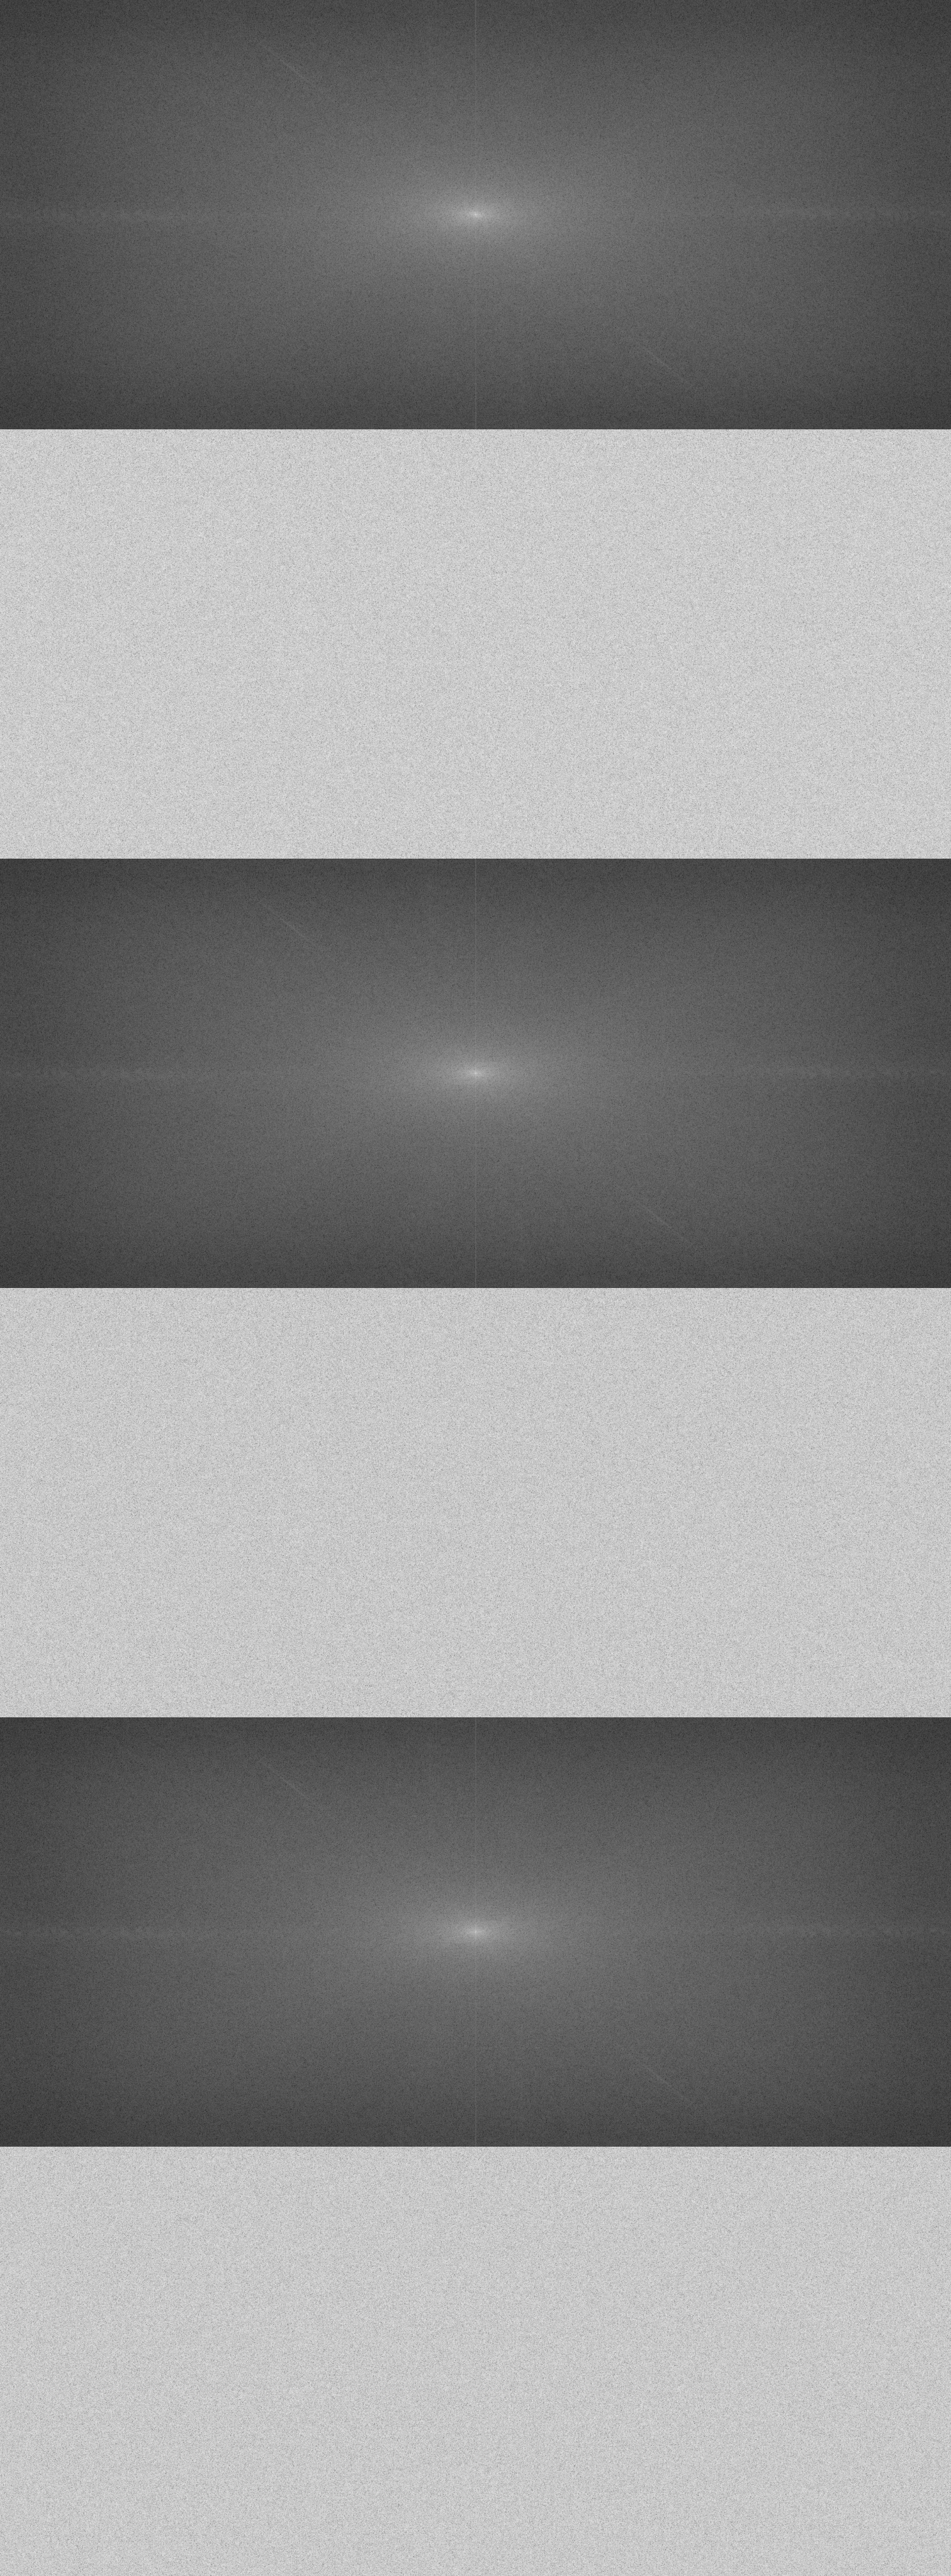
\includegraphics[width=1.0\textwidth,height=65em]{./images/mask_effect/regular_fourier_vs_modulated.png}
    \caption{effect of modulation on fourier visualization}
    \label{fig:modulation effect}
  \end{figure}
  \clearpage % End the page
}


\afterpage{%
  \clearpage % Start a new page
  \thispagestyle{empty} % No header/footer on this page
  \begin{figure}[p]
    \centering
	\captionsetup{justification=centering}
    \includegraphics[width=1.0\textwidth,height=65em]{./images/coded_diffractions_measurements_sat_phone/measurements.png}
    \caption{Measurements on DC\textregistered\space Universe Characters Due to a Random Modulation Plate from Top to Buttom: 
    Red Channel, Green Channel, Blue Channel, and Full RGB}
    \label{fig:coded_diffractions_measurements_dc}
  \end{figure}
  \clearpage % End the page
}




% \input{./tikz/error_T_max=400_steps=1_sat_phone.tex}

\afterpage{%
  \clearpage % Start a new page
  \thispagestyle{empty} % No header/footer on this pages
  \begin{figure}[p]
    \centering
	\captionsetup{justification=centering}
    \includegraphics[width=1.0\textwidth,height=65em]{./images/coded_diffractions_measurements_zoomed_sat_phone/measurements.png}
    \caption{Measurements on DC\textregistered\space Universe Characters Due to a Random Modulation Plate from Top to Buttom: 
    Red Channel, Green Channel, Blue Channel, and Full RGB Zoomed Version}
    \label{fig:coded_diffractions_measurements_zoomed_dc}
  \end{figure}
  \clearpage % End the page
}



\afterpage{%
  \clearpage % Start a new page
  \thispagestyle{empty} % No header/footer on this page
  \begin{figure}[p]
    \centering
	\captionsetup{justification=centering}
    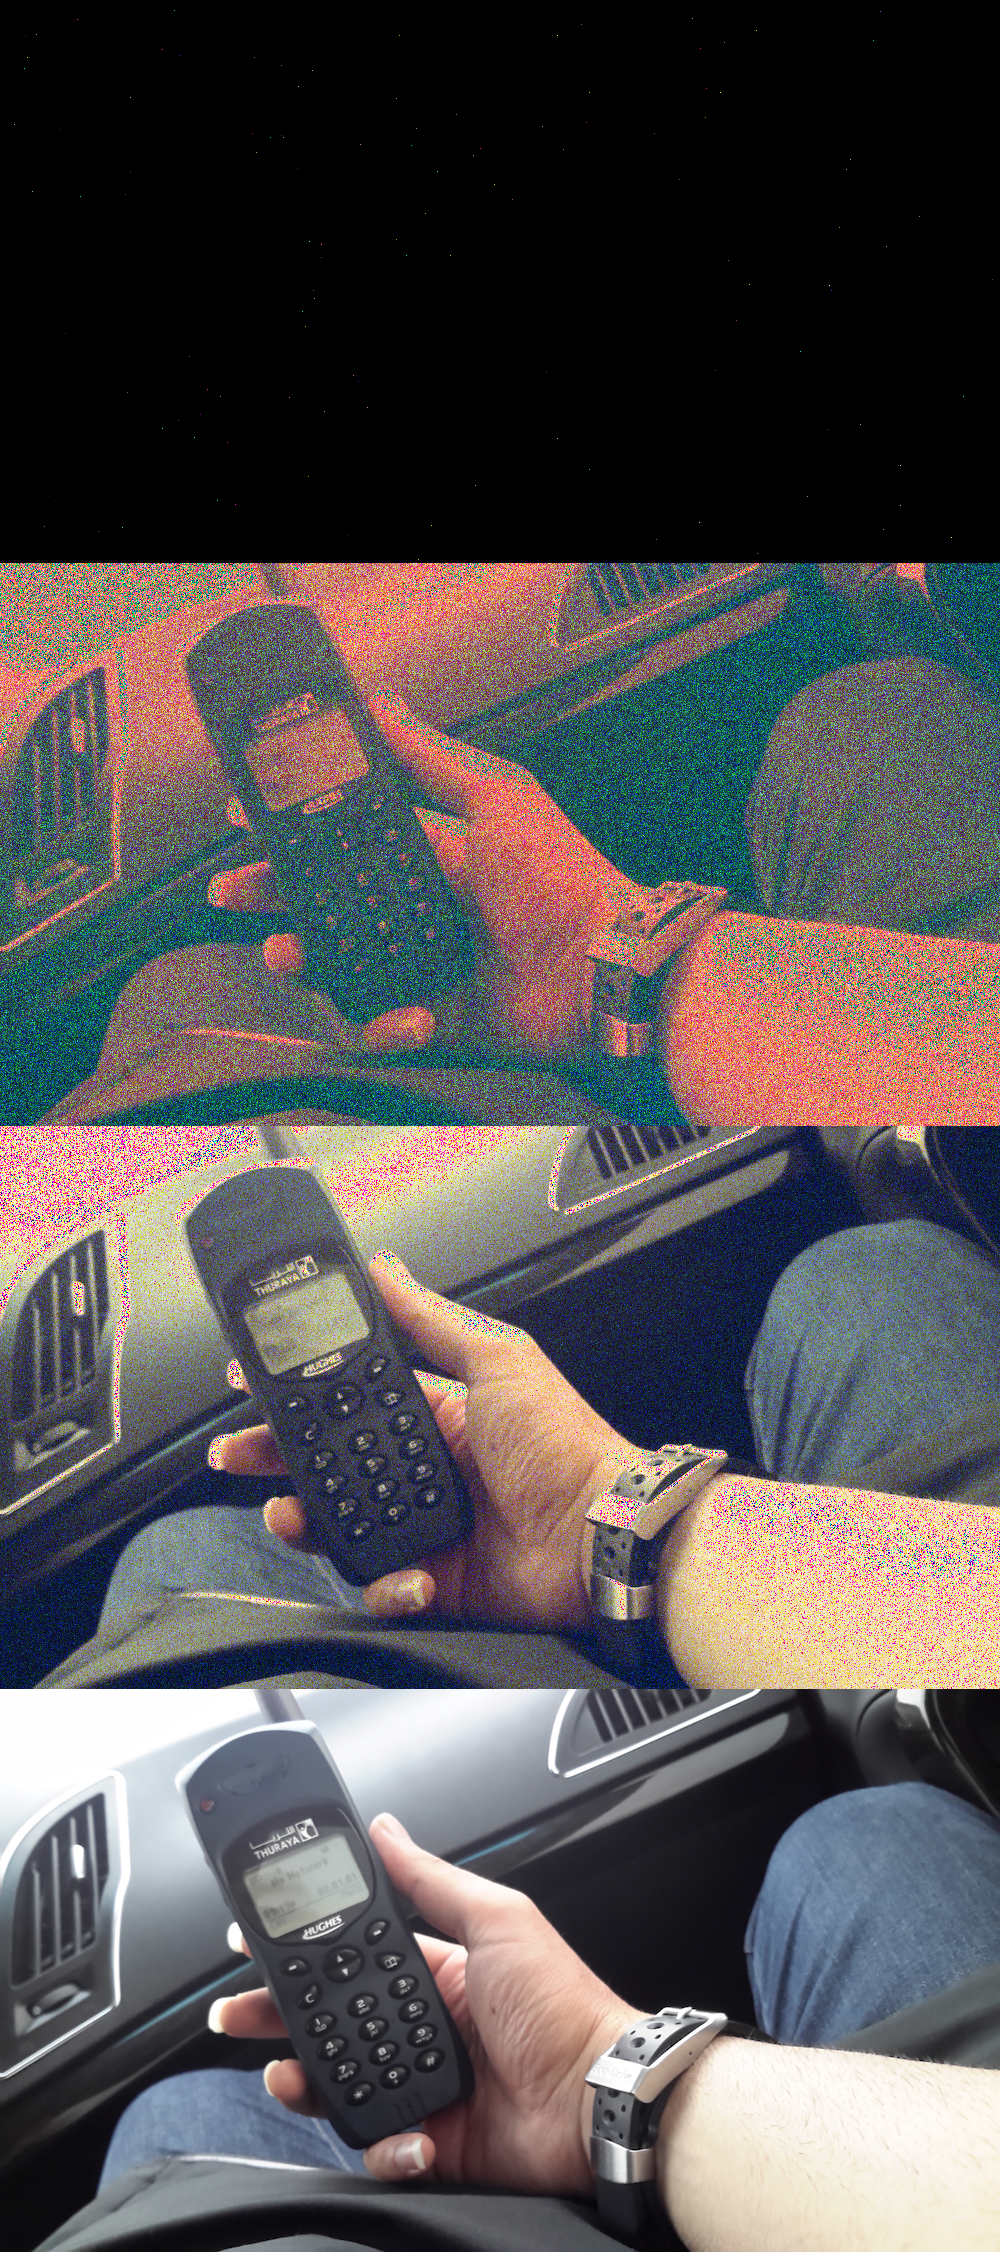
\includegraphics[width=1.0\textwidth,height=65em]{./images/wf_sat_phone/000_123_134_original.png}
    \caption{WF Using Coded Diffraction Patterns on the Sat Phone Image from Top to Buttom: After Initialization, 
	at Iteration $=123$, at Iteration $=134$, and the Original Image}
    \label{fig:wf_dc/0_121_132_original}
  \end{figure}
  \clearpage % End the page
}

\afterpage{%
  \clearpage % Start a new page
  \thispagestyle{empty} % No header/footer on this page
  \begin{figure}[p]
    \centering
	\captionsetup{justification=centering}
    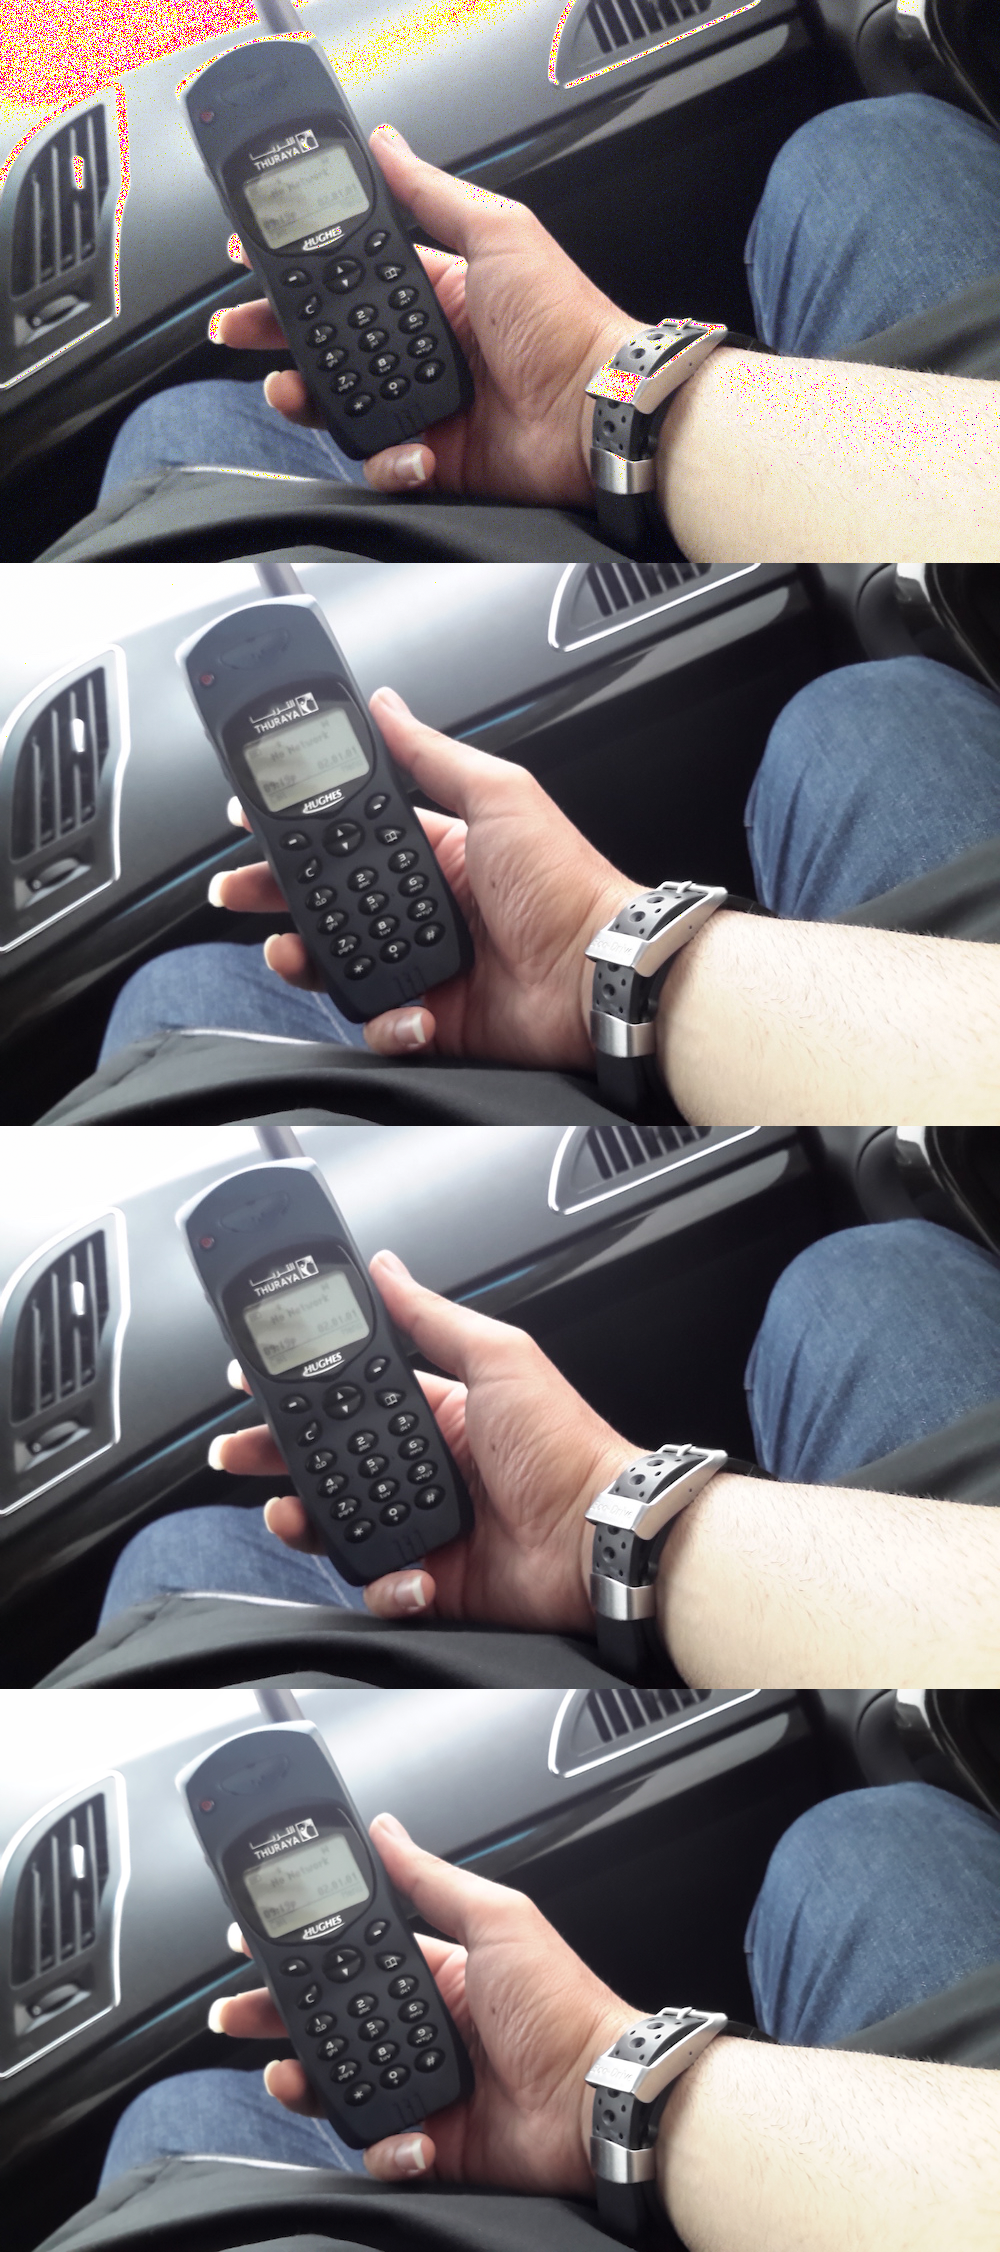
\includegraphics[width=1.0\textwidth,height=65em]{./images/wf_sat_phone/142_164_499_original.png}
    \caption{WF Using Coded Diffraction Patterns on the Sat Phone Image from Top to Buttom: At Iteration $=142$, 
    at Iteration $=164$, at Iteration $=499$, and the Original Image}
    \label{fig:wf_142_164_499_original}
  \end{figure}
  \clearpage % End the page
}





% what a mess \cite{papa_rudin}


\afterpage{%
  \clearpage % Start a new page
  \begin{table}
    \centering
    \begin{tabular}{||l l||} 
     \hline
     General 		                	&  						                                            \\ [0.5ex] 
     \hline\hline
     Processor 	         		 			& Intel(R) Xeon(R)                                       	\\
     Accelerator 			 	       		& NVIDIA  	                                              \\ 
     Operating System   			    & GNU/Linux(Ubuntu) 	                                   	\\
     Memory 	               			& 32617768 kB                                            	\\ [1ex] 
     \hline
     \hline
     Processor Details 	      		&  						                                            \\ [0.5ex] 
     \hline\hline
     Architecture     			 			& X86\_64                                               	\\ 
     CPU op-mode(s)         			& 32-bit, 64-bit 	                                      	\\
     Address sizes                & 46 bits physical, 48 bits virtual  		                  \\
     Byte Order                   & Little Endian  	                                        \\ 
     CPU(s):                      & 8 	 	                                                  \\
     On-line CPU(s) list:         & 0-7  	                                              	  \\
     Vendor ID:                   & GenuineIntel 	                                        	\\
     Model name:                  & Intel(R) Xeon(R) CPU E5-1630 v3 at 3.70GHz  	        	\\
     Thread(s) per core:          & 2                                                       \\
     Core(s) per socket:          & 4                                                   		\\
     Socket(s):                   & 1 	                                                	  \\
     CPU max MHz:                 & 3800.0000 	                                         	  \\
     CPU min MHz:                 & 1200.0000                                         	  	\\
     L1d Cache:                   & 128 KiB (4 instances)                           	    	\\
     L1i Cache:                   & 128 KiB (4 instances) 	 	                              \\
     L2 Cache:                    & 1 MiB (4 instances) 	                                 	\\
     L3 Cache:                    & 10 MiB (1 instance) 	 	                                \\
     NUMA node(s):                & 1                                               	 	    \\
     Optimization Flags           & Please Refer to the Intel Brochure for the Details  		\\[1ex] 
     \hline
     \hline
     Accelerator Details 			    &  					                                            	\\[0.5ex] 
     \hline\hline
     Full Designation 	    			& NVIDIA GeForce RTX 2080 Ti 	                            \\ 
     Memory   	              		& 11264 MiB 	                                           	\\
     CUDA Version:                & 12.2  	                                               	\\
     width:                       & 64 bits                                                 \\
     clock:                       & 33 MHz 	                                                \\[1ex] 
     \hline
     \hline
     Numerical Framework Details	&  				                                            		\\[0.5ex] 
     \hline\hline
     python                       & 3.10.12                                                 \\
     numpy                        & 1.25.2  		                                            \\
     scipy                        & 1.11.1  		                                            \\
     matplotlib                   & 3.7.2   		                                            \\
     scikit-learn                 & 1.3.0  		                                              \\
     scikit-image                 & 0.21.0  		                                            \\
     pytorch                      & 2.0.0			 			 	                                      \\ 
     pytorch-cuda                 & 11.7 	 	                                                \\
     \LaTeX \space Distribution   & Mac\TeX			 			 	                                    \\
     \LaTeX \space Engine/Recipe  & Auto Recipe in VS-Code \LaTeX \space Extension		      \\ [1ex] 
     \hline
    \end{tabular}
    \caption{Software and Hardware that were used}
    % \label{tab:formulation}
    \end{table}
  \clearpage % End the page
}


 
\nocite{*}
\backmatter
\printindex
\printbibliography

\end{document}